\chapter{Điện từ trường và cảm ứng điện từ}

\begin{vd}[Dịch chuyển nam châm]
Hai thanh nam châm giống hệt nhau được đặt cách nhau như hình vẽ.
\begin{center}


\tikzset{every picture/.style={line width=0.75pt}} %set default line width to 0.75pt        

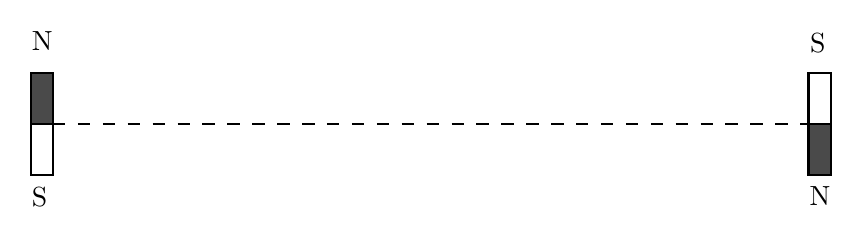
\begin{tikzpicture}[x=0.75pt,y=0.75pt,yscale=-1,xscale=1]
%uncomment if require: \path (0,300); %set diagram left start at 0, and has height of 300

%Shape: Rectangle [id:dp5022362522100339] 
\draw  [color={rgb, 255:red, 0; green, 0; blue, 0 }  ,draw opacity=1 ][fill={rgb, 255:red, 74; green, 74; blue, 74 }  ,fill opacity=1 ] (129,123.4) -- (139.7,123.4) -- (139.7,148) -- (129,148) -- cycle ;
%Shape: Rectangle [id:dp35545825300116207] 
\draw   (129,148) -- (139.7,148) -- (139.7,172.6) -- (129,172.6) -- cycle ;
%Straight Lines [id:da3079932428464216] 
\draw  [dash pattern={on 4.5pt off 4.5pt}]  (139.7,148) -- (503.7,148) ;
%Shape: Rectangle [id:dp6572429819042589] 
\draw   (503.7,123.4) -- (514.4,123.4) -- (514.4,148) -- (503.7,148) -- cycle ;
%Shape: Rectangle [id:dp5289011457931987] 
\draw  [fill={rgb, 255:red, 74; green, 74; blue, 74 }  ,fill opacity=1 ] (503.7,148) -- (514.4,148) -- (514.4,172.6) -- (503.7,172.6) -- cycle ;


% Text Node
\draw (128,102) node [anchor=north west][inner sep=0.75pt]   [align=left] {N};
% Text Node
\draw (128,177) node [anchor=north west][inner sep=0.75pt]   [align=left] {S};
% Text Node
\draw (502.7,176.6) node [anchor=north west][inner sep=0.75pt]   [align=left] {N};
% Text Node
\draw (503,103) node [anchor=north west][inner sep=0.75pt]   [align=left] {S};


\end{tikzpicture}
\end{center}
Trong trường hợp nào dưới đây cần tốn nhiều công hơn? Và tốn nhiều hơn bao nhiêu lần?
\begin{enumerate}[1)]
\item Trục của nam châm bên phải xoay chậm đi $180^\circ$ sao cho hai moment lưỡng cực từ song song nhau.
 \item Nam châm bên phải được đưa ra xa vô cực dọc theo đường nối hai nam châm.
 \end{enumerate}
\end{vd}

\begin{loigiai} \\
Chúng ta cần chú ý rằng, trong cả hai trường hợp, công thực hiện đều là tăng thế năng tương tác từ.\\
Xét thí nghiệm sau: Nam châm ở bên phải được đưa đi rất xa khỏi nam châm bên trái dọc theo đường nối hai nam châm, công thực hiện để chống lại lực hút giữa hai nam châm được đặt là một đơn vị. Đây là công cần thực hiện trong câu $2)$.\\
Tiếp theo, nam châm ở bên phải sau khi được đưa ra xa vô cùng sẽ được quay một góc $180^\circ$, không có công nào được thực hiện trong quá trình này bởi vì tương tác giữa hai nam châm lúc này là không đáng kể. Cuối cùng, nam châm sau khi xoay được đưa trở lại vị trí ban đầu của nó. Theo tính đối xứng, phần công thực hiện để chống lại lực đẩy trong quá tình này cũng là một đơn vị. Đây là công cần thực hiện ở phần $1)$ và minh chứng rằng công cần thực hiện trong quá trình này là hai đơn vị.\\
Trường điện từ là trường thế, tức là mọi thăng giáng của năng lượng tương tác từ chỉ phụ thuộc và vị trí đầu và vị trí cuối của vật chứ không phụ thuộc vào quá trình chúng ta di chuyển vật như thế nào. Do đó, chúng ta có thể suy ra, nếu chúng ta quay nam châm đi $180^o$ từ vị trí ban đầu, phần công cần thực hiện cũng là hai đơn vị. \\
Tóm lại, phần $1)$ tốn một phần công nhiều gấp đôi phần $2)$.
\end{loigiai}

\begin{vd}[Dòng điện do các electron chạy qua miền có từ trường]
Các electron và một vài nguyên tử có moment động lượng riêng được gọi là spin $(\ot{S})$, các spin đó có độ lớn không đổi nhưng hướng của chúng có thể thay đổi do moment của ngoại lực. Liên kết với các spin là các moment từ làm cho chúng giống như những lưỡng cực từ $\ot{m}=\mu_{B}\ot{S}$ với $\mu_{B}$ là một hằng số gọi là \textbf{magneton}. Để đơn giản, chúng ta giả sử rằng các electron và các nguyên tử có dùng độ lớn spin $S$ và \textbf{magneton}.
\begin{enumerate}[1) ]
    \item Tham khảo hình $A$ dưới đây. Lưỡng cực $A$ ở tại $\ot{r}=0$ và dọc theo $\ot{z_0}$, và lưỡng cực $B$ ở tại $\ot{r}=\alpha\ot{x_0}$ và dọc theo $\ot{y_0}$. Tìm moment lực do lưỡng cực $A$ tác dụng lên lưỡng cực $B$.
    \item Tìm hướng của lưỡng cực $B$ sau một khoảng thời gian ngắn $\Delta t$, giả sử rằng hướng của lưỡng cực $A$ vẫn không thay đổi.
    \item Hình $B$ là sơ đồ của một miền từ trường trong $(x_0,x_0+2b)$ có chứa nhiều nguyên tử (lưỡng cực $B$). Hướng của các lưỡng cực được chỉ ra như hình vẽ. Các lưỡng cực $B$ được cố định ở các khoảng cách bằng nhau trên trục $x$ (trong miền không gian là $2b$ có $10^4$ lưỡng cực $B$). Một electron (lưỡng cực $A$) bay và tác động lên lưỡng cực B như là câu trả lời của bạn ở phần $(2$). Hình $C$  cho biết góc ban đầu của các lưỡng cực. Lưỡng cực ở $x_0+b$ dọc theo $\ot{y_0}$, lưỡng cực ở $x\leq x_0$ dọc theo $-\ot{x_0}$ và lưỡng cực ở $x\geq x_0+2b$ dọc theo $\ot{x_0}$. Các lưỡng cực dọc theo $-\ot{x_0}$ còn có thể quay. Các lưỡng cực dọc theo $\ot{x_0}$ thì không thể quay, ngoại trừ những lưỡng cực ở gần mép (rìa) của miền có thể quay tự do một chút. Cho dòng điện bởi các hạt tải electron là $I$, tìm tốc độ chuyển động khi qua tâm miền khi dòng điện được bật lên. (cho rằng điện tích của electron là $e$ đã biết). 
    \item Tìm thời gian cần thiết để vượt qua toàn bộ miền.
    \end{enumerate}
(\textit{Gợi ý:} Từ trường $\ot{B}(\ot{r})$ tại vị trí $\ot{r}$ do lưỡng cực từ $\ot{m}$ tại gốc tọa độ được cho bởi $\ot{B}(\ot{r})=\dfrac{\mu_0}{4\pi r^3}\left[\dfrac{3(\ot{m}\cdot\ot{r})\ot{r}}{r^2}-\ot{m}\right]$. Moment lực $\ot{N}$ của từ trường hướng $\ot{B}$ tác dụng lên lưỡng cực $\ot{m}$ là $\ot{N}=\ot{m}\times\ot{B}$.)
\begin{center}



\tikzset{every picture/.style={line width=0.75pt}} %set default line width to 0.75pt        

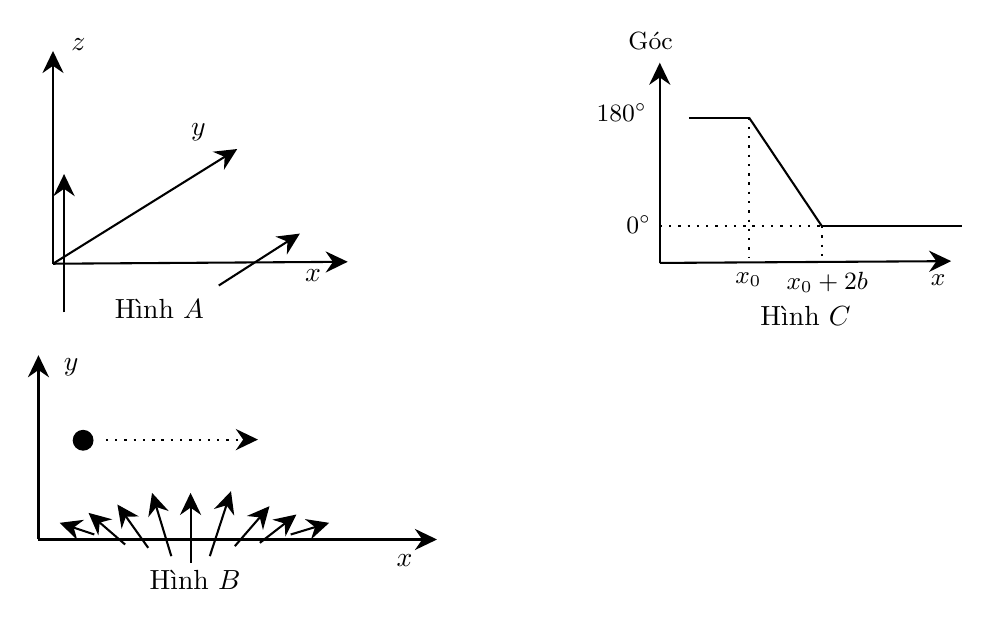
\begin{tikzpicture}[x=0.75pt,y=0.75pt,yscale=-1,xscale=1]
%uncomment if require: \path (0,300); %set diagram left start at 0, and has height of 300

%Straight Lines [id:da4492620820243536] 
\draw    (29,125.45) -- (29,25.95) ;
\draw [shift={(29,22.95)}, rotate = 450] [fill={rgb, 255:red, 0; green, 0; blue, 0 }  ][line width=0.08]  [draw opacity=0] (10.72,-5.15) -- (0,0) -- (10.72,5.15) -- (7.12,0) -- cycle    ;
%Straight Lines [id:da3879660645016081] 
\draw    (29,125.45) -- (115.2,71.77) ;
\draw [shift={(117.75,70.19)}, rotate = 508.09] [fill={rgb, 255:red, 0; green, 0; blue, 0 }  ][line width=0.08]  [draw opacity=0] (10.72,-5.15) -- (0,0) -- (10.72,5.15) -- (7.12,0) -- cycle    ;
%Straight Lines [id:da3664498690573632] 
\draw    (34.33,148.91) -- (34.33,85.23) ;
\draw [shift={(34.33,82.23)}, rotate = 450] [fill={rgb, 255:red, 0; green, 0; blue, 0 }  ][line width=0.08]  [draw opacity=0] (10.72,-5.15) -- (0,0) -- (10.72,5.15) -- (7.12,0) -- cycle    ;
%Straight Lines [id:da03392174383237889] 
\draw    (29,125.45) -- (168,124.54) ;
\draw [shift={(171,124.52)}, rotate = 539.63] [fill={rgb, 255:red, 0; green, 0; blue, 0 }  ][line width=0.08]  [draw opacity=0] (10.72,-5.15) -- (0,0) -- (10.72,5.15) -- (7.12,0) -- cycle    ;
%Straight Lines [id:da667880177313547] 
\draw    (108.88,135.94) -- (145.4,112.56) ;
\draw [shift={(147.93,110.94)}, rotate = 507.37] [fill={rgb, 255:red, 0; green, 0; blue, 0 }  ][line width=0.08]  [draw opacity=0] (10.72,-5.15) -- (0,0) -- (10.72,5.15) -- (7.12,0) -- cycle    ;


%Straight Lines [id:da9465992584207192] 
\draw    (22,258.31) -- (22,172.53) ;
\draw [shift={(22,169.53)}, rotate = 450] [fill={rgb, 255:red, 0; green, 0; blue, 0 }  ][line width=0.08]  [draw opacity=0] (10.72,-5.15) -- (0,0) -- (10.72,5.15) -- (7.12,0) -- cycle    ;
%Straight Lines [id:da9778405244192359] 
\draw    (22,258.31) -- (211,258.31) ;
\draw [shift={(214,258.31)}, rotate = 180] [fill={rgb, 255:red, 0; green, 0; blue, 0 }  ][line width=0.08]  [draw opacity=0] (10.72,-5.15) -- (0,0) -- (10.72,5.15) -- (7.12,0) -- cycle    ;
%Straight Lines [id:da3787820827861692] 
\draw    (95.28,269.55) -- (95.28,238.85) ;
\draw [shift={(95.28,235.85)}, rotate = 450] [fill={rgb, 255:red, 0; green, 0; blue, 0 }  ][line width=0.08]  [draw opacity=0] (10.72,-5.15) -- (0,0) -- (10.72,5.15) -- (7.12,0) -- cycle    ;
%Straight Lines [id:da6658921469128833] 
\draw    (104.55,266.34) -- (113.82,237.9) ;
\draw [shift={(114.75,235.05)}, rotate = 468.06] [fill={rgb, 255:red, 0; green, 0; blue, 0 }  ][line width=0.08]  [draw opacity=0] (10.72,-5.15) -- (0,0) -- (10.72,5.15) -- (7.12,0) -- cycle    ;
%Straight Lines [id:da4077367348968337] 
\draw    (86,266.34) -- (77.6,238.72) ;
\draw [shift={(76.72,235.85)}, rotate = 433.08000000000004] [fill={rgb, 255:red, 0; green, 0; blue, 0 }  ][line width=0.08]  [draw opacity=0] (10.72,-5.15) -- (0,0) -- (10.72,5.15) -- (7.12,0) -- cycle    ;
%Straight Lines [id:da9033165151070539] 
\draw    (74.87,262.33) -- (61.77,243.91) ;
\draw [shift={(60.03,241.47)}, rotate = 414.57] [fill={rgb, 255:red, 0; green, 0; blue, 0 }  ][line width=0.08]  [draw opacity=0] (10.72,-5.15) -- (0,0) -- (10.72,5.15) -- (7.12,0) -- cycle    ;
%Straight Lines [id:da5709523099777032] 
\draw    (116.61,261.52) -- (131.34,244.54) ;
\draw [shift={(133.3,242.27)}, rotate = 490.93] [fill={rgb, 255:red, 0; green, 0; blue, 0 }  ][line width=0.08]  [draw opacity=0] (10.72,-5.15) -- (0,0) -- (10.72,5.15) -- (7.12,0) -- cycle    ;
%Straight Lines [id:da44092929640949885] 
\draw    (128.67,259.92) -- (143.92,248.12) ;
\draw [shift={(146.29,246.28)}, rotate = 502.27] [fill={rgb, 255:red, 0; green, 0; blue, 0 }  ][line width=0.08]  [draw opacity=0] (10.72,-5.15) -- (0,0) -- (10.72,5.15) -- (7.12,0) -- cycle    ;
%Straight Lines [id:da6575017322814591] 
\draw    (63.74,260.72) -- (48.38,247.44) ;
\draw [shift={(46.12,245.48)}, rotate = 400.86] [fill={rgb, 255:red, 0; green, 0; blue, 0 }  ][line width=0.08]  [draw opacity=0] (10.72,-5.15) -- (0,0) -- (10.72,5.15) -- (7.12,0) -- cycle    ;
%Straight Lines [id:da09095595030926118] 
\draw    (48.9,255.91) -- (35.05,251.25) ;
\draw [shift={(32.2,250.29)}, rotate = 378.59000000000003] [fill={rgb, 255:red, 0; green, 0; blue, 0 }  ][line width=0.08]  [draw opacity=0] (10.72,-5.15) -- (0,0) -- (10.72,5.15) -- (7.12,0) -- cycle    ;
%Straight Lines [id:da8512931349485788] 
\draw    (143.51,255.91) -- (159.19,251.16) ;
\draw [shift={(162.06,250.29)}, rotate = 523.1600000000001] [fill={rgb, 255:red, 0; green, 0; blue, 0 }  ][line width=0.08]  [draw opacity=0] (10.72,-5.15) -- (0,0) -- (10.72,5.15) -- (7.12,0) -- cycle    ;
%Straight Lines [id:da14846896037639024] 
\draw  [dash pattern={on 0.84pt off 2.51pt}]  (54.46,210.18) -- (124.74,210.18) ;
\draw [shift={(127.74,210.18)}, rotate = 180] [fill={rgb, 255:red, 0; green, 0; blue, 0 }  ][line width=0.08]  [draw opacity=0] (10.72,-5.15) -- (0,0) -- (10.72,5.15) -- (7.12,0) -- cycle    ;
%Straight Lines [id:da5150132226935988] 
\draw    (321.34,125.07) -- (321.34,31.59) ;
\draw [shift={(321.34,28.59)}, rotate = 450] [fill={rgb, 255:red, 0; green, 0; blue, 0 }  ][line width=0.08]  [draw opacity=0] (10.72,-5.15) -- (0,0) -- (10.72,5.15) -- (7.12,0) -- cycle    ;
%Straight Lines [id:da35548173749016] 
\draw    (321.34,125.07) -- (458.74,124.22) ;
\draw [shift={(461.74,124.2)}, rotate = 539.64] [fill={rgb, 255:red, 0; green, 0; blue, 0 }  ][line width=0.08]  [draw opacity=0] (10.72,-5.15) -- (0,0) -- (10.72,5.15) -- (7.12,0) -- cycle    ;

%Straight Lines [id:da6685787959685461] 
\draw    (335.38,55.03) -- (364.34,55.03) ;
%Straight Lines [id:da5287919204143205] 
\draw    (399.43,107.34) -- (467,107.34) ;
%Straight Lines [id:da9848832862195076] 
\draw    (364.34,55.03) -- (399.43,107.34) ;
%Straight Lines [id:da2528288642770211] 
\draw  [dash pattern={on 0.84pt off 2.51pt}]  (399.43,107.34) -- (399.43,124.78) ;
%Straight Lines [id:da7577180254188209] 
\draw  [dash pattern={on 0.84pt off 2.51pt}]  (364.34,55.03) -- (364.34,122.46) ;
%Straight Lines [id:da3431528400294237] 
\draw  [dash pattern={on 0.84pt off 2.51pt}]  (321.34,107.34) -- (399.43,107.34) ;

%Shape: Circle [id:dp16187367515635387] 
\draw  [fill={rgb, 255:red, 0; green, 0; blue, 0 }  ,fill opacity=1 ] (39,210.51) .. controls (39,208.02) and (41.02,206) .. (43.51,206) .. controls (46,206) and (48.02,208.02) .. (48.02,210.51) .. controls (48.02,213) and (46,215.02) .. (43.51,215.02) .. controls (41.02,215.02) and (39,213) .. (39,210.51) -- cycle ;


% Text Node
\draw (149.02,126.8) node [anchor=north west][inner sep=0.75pt]    {$x$};
% Text Node
\draw (94,56.41) node [anchor=north west][inner sep=0.75pt]    {$y$};
% Text Node
\draw (36.31,15.66) node [anchor=north west][inner sep=0.75pt]    {$z$};
% Text Node
\draw (57.25,141.15) node [anchor=north west][inner sep=0.75pt]   [align=left] {Hình $\displaystyle A$};
% Text Node
\draw (450.47,129.51) node [anchor=north west][inner sep=0.75pt]  [font=\small]  {$x$};
% Text Node
\draw (356.21,128.35) node [anchor=north west][inner sep=0.75pt]  [font=\small]  {$x_{0}$};
% Text Node
\draw (381.01,128.22) node [anchor=north west][inner sep=0.75pt]  [font=\small]  {$x_{0} +2b$};
% Text Node
\draw (304.77,12.22) node [anchor=north west][inner sep=0.75pt]  [font=\small] [align=left] {Góc};
% Text Node
\draw (303.75,100.68) node [anchor=north west][inner sep=0.75pt]  [font=\small]  {$0^{\circ }$};
% Text Node
\draw (289.36,46.63) node [anchor=north west][inner sep=0.75pt]  [font=\small]  {$180^{\circ }$};
% Text Node
\draw (368.35,144.55) node [anchor=north west][inner sep=0.75pt]   [align=left] {Hình $\displaystyle C$};
% Text Node
\draw (193.09,264.07) node [anchor=north west][inner sep=0.75pt]    {$x$};
% Text Node
\draw (32.7,169.42) node [anchor=north west][inner sep=0.75pt]    {$y$};
% Text Node
\draw (74.06,271.51) node [anchor=north west][inner sep=0.75pt]   [align=left] {Hình $\displaystyle B$};


\end{tikzpicture}
\end{center}
\end{vd}

\begin{loigiai}
\begin{enumerate}[1)]
    \item Moment lực là
    \[\ot{\tau}=\dfrac{\mu_0}{4\pi a^3}\ot{m_{\mathrm{A}}}\times\ot{m_{\mathrm{B}}}=-\dfrac{\mu_0(\mu_{\mathrm{B}}S)^2}{4\pi a^3}\ot{x_0}~\text{vuông góc với}~\ot{m_{\mathrm{B}}}.\]
    \begin{center}
\tikzset{every picture/.style={line width=0.75pt}} %set default line width to 0.75pt        

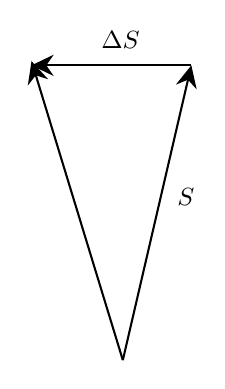
\begin{tikzpicture}[x=0.75pt,y=0.75pt,yscale=-1,xscale=1]
%uncomment if require: \path (0,300); %set diagram left start at 0, and has height of 300

%Straight Lines [id:da9599488966246523] 
\draw    (239,210.33) -- (195.88,69.15) ;
\draw [shift={(195,66.28)}, rotate = 433.01] [fill={rgb, 255:red, 0; green, 0; blue, 0 }  ][line width=0.08]  [draw opacity=0] (10.72,-5.15) -- (0,0) -- (10.72,5.15) -- (7.12,0) -- cycle    ;
%Straight Lines [id:da4147110006600949] 
\draw    (239,210.33) -- (271.32,71.23) ;
\draw [shift={(272,68.31)}, rotate = 463.08] [fill={rgb, 255:red, 0; green, 0; blue, 0 }  ][line width=0.08]  [draw opacity=0] (10.72,-5.15) -- (0,0) -- (10.72,5.15) -- (7.12,0) -- cycle    ;
%Straight Lines [id:da5247662187374407] 
\draw    (272,68.31) -- (198,68.31) ;
\draw [shift={(195,68.31)}, rotate = 360] [fill={rgb, 255:red, 0; green, 0; blue, 0 }  ][line width=0.08]  [draw opacity=0] (10.72,-5.15) -- (0,0) -- (10.72,5.15) -- (7.12,0) -- cycle    ;

% Text Node
\draw (263.75,125.93) node [anchor=north west][inner sep=0.75pt]  [font=\small]  {$S$};
% Text Node
\draw (227.13,50.66) node [anchor=north west][inner sep=0.75pt]  [font=\small]  {$\Delta S$};


\end{tikzpicture}
    \end{center}
    \item Moment lực là nguyên nhân làm cho $\ot{S_{\mathrm{B}}}$ quay trong mặt phẳng $x-y$, và tốc độ góc được cho bởi $\tau=S\omega$.\\
    Góc hợp với trục $y$ là
    \[\Delta\theta=\omega\Delta t=\dfrac{\mu_0}{4\pi a^3}\mu_{\mathrm{b}}^2S\Delta t.\]
    \item Hãy tìm số lượng electron phải vượt qua để tạo ra một spin đặc biệt để quay từ $90^\circ - \mathrm{d}\theta$ tới $90^\circ$ và từ $\theta$ tìm vị trí của spin.
    \begin{align*}
        \left(\dfrac{I}{e}\Delta\theta\right)\mathrm{d}t&=\mathrm{d}\theta=\dfrac{\pi}{2b}\mathrm{d}x.\\
        v&=\dfrac{\mathrm{d}x}{\mathrm{d}t}=\dfrac{2bI}{\pi e}\Delta\theta=\dfrac{\mu_0}{2e\pi^2a^3}bI\mu^2_{\mathrm{b}}S\Delta t.
    \end{align*}
    \begin{center}
 

\tikzset{every picture/.style={line width=0.75pt}} %set default line width to 0.75pt        

\begin{tikzpicture}[x=0.75pt,y=0.75pt,yscale=-1,xscale=1]
%uncomment if require: \path (0,300); %set diagram left start at 0, and has height of 300

%Straight Lines [id:da6598694439969128] 
\draw    (160.84,208.69) -- (160.84,70.81) ;
\draw [shift={(160.84,67.81)}, rotate = 450] [fill={rgb, 255:red, 0; green, 0; blue, 0 }  ][line width=0.08]  [draw opacity=0] (10.72,-5.15) -- (0,0) -- (10.72,5.15) -- (7.12,0) -- cycle    ;
%Straight Lines [id:da6810032084360103] 
\draw    (160.84,208.69) -- (472.21,207.43) ;
\draw [shift={(475.21,207.42)}, rotate = 539.77] [fill={rgb, 255:red, 0; green, 0; blue, 0 }  ][line width=0.08]  [draw opacity=0] (10.72,-5.15) -- (0,0) -- (10.72,5.15) -- (7.12,0) -- cycle    ;

%Straight Lines [id:da7910578702301538] 
\draw    (192.28,106.43) -- (257.12,106.43) ;
%Straight Lines [id:da13220931113446555] 
\draw    (335.71,182.8) -- (487,182.8) ;
%Straight Lines [id:da17089054030238615] 
\draw    (257.12,106.43) -- (335.71,182.8) ;
%Straight Lines [id:da6135971059333494] 
\draw  [dash pattern={on 0.84pt off 2.51pt}]  (335.71,182.8) -- (335.71,208.26) ;
%Straight Lines [id:da40308318362058393] 
\draw  [dash pattern={on 0.84pt off 2.51pt}]  (257.12,106.43) -- (257.12,208.33) ;
%Straight Lines [id:da29183622476100535] 
\draw  [dash pattern={on 0.84pt off 2.51pt}]  (160.84,182.8) -- (335.71,182.8) ;
%Straight Lines [id:da5842701379801969] 
\draw  [dash pattern={on 0.84pt off 2.51pt}]  (253.12,106.43) -- (269,106.43) ;
%Straight Lines [id:da24335614573950703] 
\draw  [dash pattern={on 0.84pt off 2.51pt}]  (503,182.8) -- (346,182.8) ;
%Straight Lines [id:da8478129293644809] 
\draw  [dash pattern={on 0.84pt off 2.51pt}]  (267.41,106.43) -- (346,182.8) ;

% Text Node
\draw (455.42,213.21) node [anchor=north west][inner sep=0.75pt]  [font=\small]  {$x$};
% Text Node
\draw (250.84,211.74) node [anchor=north west][inner sep=0.75pt]  [font=\small]  {$x_{0}$};
% Text Node
\draw (321.57,209.55) node [anchor=north west][inner sep=0.75pt]  [font=\small]  {$x_{0} +2b$};
% Text Node
\draw (146.47,51.37) node [anchor=north west][inner sep=0.75pt]  [font=\small] [align=left] {Góc};
% Text Node
\draw (141.75,176.34) node [anchor=north west][inner sep=0.75pt]  [font=\small]  {$0^{\circ }$};
% Text Node
\draw (129.45,97.42) node [anchor=north west][inner sep=0.75pt]  [font=\small]  {$180^{\circ }$};
% Text Node
\draw (296.47,241.27) node [anchor=north west][inner sep=0.75pt]   [align=left] {Hình $\displaystyle C$};


\end{tikzpicture}
    \end{center}
    \item 
    \[t=\dfrac{2b}{v}=\dfrac{4e\pi^2a^3}{\mu_0I\mu^2_{\mathrm{b}}S\Delta t}.\]
\end{enumerate}
\end{loigiai}

\begin{vd}[Độ từ hóa]
\begin{enumerate}[1)]
    \item Một cái đĩa có bán kính $R$ và bề dày $d(\ll R)$ được từ hóa đều với từ tính vuông góc với mặt đĩa. Tìm từ trường tại điểm $O$ trên trục đi qua tâm đĩa và ở cách tâm đĩa một khoảng $h$. 
    \item Một hình trụ dài được từ hóa trung bình với độ từ hóa $\ot{M}$ dọc theo trục hình trụ. Tìm từ trường bên trong và bên ngoài của hình trụ đó.
\end{enumerate}
\end{vd}
\begin{loigiai}
\begin{enumerate}[1) ]
    \item Mật độ dòng điện liên kết của đĩa là:
    \[K=-\ot{M}\times\ot{n}=-M,\]
    Dòng điện là: $I=Jd=-Md,$\\
    Từ trường:
    \[B(z=h)=\dfrac{\mu_0R^2I}{2(R^2+h^2)^{\dfrac{3}{2}}}=-\dfrac{\mu_0R^2Md}{2(R^2+h^2)^{\dfrac{3}{2}}}.\]
    \item Mật độ dòng điện liên kết là $K=-\ot{M}\times\ot{n}=-M$, đó là trên thành bên của hình trụ.\\
    Bài toán này khi đó giống như một ống solenoid dài. Sử dụng vòng Ampere nhỏ ta có ở bên trong $B=\mu_0K=\mu_0M$ và ở bên ngoài $B=0$.
\end{enumerate}
\end{loigiai} 

\begin{vd}[Các đơn cực từ]
    \begin{center}
      

\tikzset{every picture/.style={line width=0.75pt}} %set default line width to 0.75pt        

\begin{tikzpicture}[x=0.75pt,y=0.75pt,yscale=-1,xscale=1]
%uncomment if require: \path (0,300); %set diagram left start at 0, and has height of 300

%Straight Lines [id:da22909332327350906] 
\draw    (240,90) -- (240,239.2) ;
%Straight Lines [id:da6765772392847864] 
\draw    (290,117.2) -- (290,184.2) ;
\draw [shift={(290,114.2)}, rotate = 90] [fill={rgb, 255:red, 0; green, 0; blue, 0 }  ][line width=0.08]  [draw opacity=0] (10.72,-5.15) -- (0,0) -- (10.72,5.15) -- (7.12,0) -- cycle    ;
%Straight Lines [id:da7347835505124456] 
\draw    (290,184.2) -- (308.02,184.2) ;
\draw [shift={(311.02,184.2)}, rotate = 180] [fill={rgb, 255:red, 0; green, 0; blue, 0 }  ][line width=0.08]  [draw opacity=0] (10.72,-5.15) -- (0,0) -- (10.72,5.15) -- (7.12,0) -- cycle    ;

% Text Node
\draw (285,95.4) node [anchor=north west][inner sep=0.75pt]    {$x$};
% Text Node
\draw (312,182.4) node [anchor=north west][inner sep=0.75pt]    {$z$};
% Text Node
\draw (252,96.4) node [anchor=north west][inner sep=0.75pt]    {$1$};
% Text Node
\draw (211,96.4) node [anchor=north west][inner sep=0.75pt]    {$2$};


\end{tikzpicture}
    \end{center}
Định lí duy nhất của lí thuyết điện từ trường chỉ ra rằng điện tích ảo (điện tích ảnh) có thể được đặt bên ngoài không gian kín, trong đó trường ảnh đó được xác định bằng cách bắt chước điều kiện biên gốc. \textbf{Trường bên trong} không gian kín đó giống như trường được tạo ra bởi các điện tích thật bên trong không gian và các điện tích ảo bên ngoài không gian đó. Đối với một mặt mà không có các điện tích tự do và dòng điện tự do, các điều kiện biên cho điện trường $\ot{E}$, điện cảm $\ot{D}$, từ trường $\ot{B}$, và cảm ứng từ $\ot{H}$ là $\ot{E^{\parallel}_1}=\ot{E^{\parallel}_2}$, $\ot{D_1^{\bot}}=\ot{D_2^{\bot}}$, $\ot{B_1^{\bot}}=\ot{B_2^{\bot}}$, $\ot{H^{\parallel}_1}=\ot{H^{\parallel}_2}$. Ở đây kí hiệu ``$\bot$'' nghĩa là thành phần vuông góc với bề mặt và ``$\parallel$'' nghĩa là thành phần song song với mặt đó.
\begin{enumerate}[1) ]
    \item Xét trường hợp một điện tích điểm $q$ trong môi trường $1$ tại khoảng cách $d$ tính từ bề mặt chung giữa hai môi trường điện môi có các hằng số điện môi tương ứng là $\varepsilon_1$ và $\varepsilon_2$. Trục $Z$ vuông góc với bề mặt chung, điện tích điểm $q$ nằm trên trục $Z$, và bề mặt chung tại $z=0$. Hai điện tích ảnh $q_1$ và $q_2$ được sử dụng để giải bài toán này. Trong môi trường $2$, điện trường bằng với những gì được tạo ra bởi một điện tích điểm $(q_1+\dfrac{q}{\varepsilon_1})$ tại điểm có tọa độ $(0,0,d)$. Điện trường ở trong môi trường $1$ bằng với điện trường toàn phần được tạo ra bởi một điện tích điểm $\dfrac{q}{\varepsilon_1}$ tại vị trí $(0,0,d)$ và một điện tích điểm $q_2$ tại vị trí $(0,0,-d)$.
    \begin{enumerate}[a) ]
        \item Áp dụng các điều kiện biên nói trên để xác định các điện tích $q_1$ và $q_2$.
        \item Xác định mật độ điện tích mặt toàn phần tại bề mặt.
        \item Kiểm tra lại kết quả của bạn bằng điều kiện đặc biệt $\varepsilon_1=\varepsilon_2$.
        \item Kiểm tra lại câu trả lời của bạn với điều kiện đặc biệt $\varepsilon_1\ll\varepsilon_2$.
    \end{enumerate}
    \item Một lưỡng cực từ được làm bằng cực nam và cực bắc. Thật thú vị, cho đến nay không có đơn cực từ, cụ thể là các vật thể chỉ mang một cực nam hoặc một cực bắc, đã từng được phát hiện. Nếu một đơn cực từ giống như một ``điện tích từ'' $g$ tồn tại, nó sẽ tạo ra một từ trường giống như một điện tích điểm điện tạo ra một điện trường. Gần đây, các hạt giả hoạt động giống như một đơn cực từ được tạo ra bởi tập hợp các chuyển động của các electron trong một kiểu vật liệu được gọi là ``chất cách điện topo'', theo lí thuyết đã được dự đoán. Hạt như vậy có thể được gây ra bởi một điện tích điểm bên ngoài. Tương tự như phần $1)$, điện tích điểm $q$ được đặt ở khoảng cách $d$ đối với một mặt giữa một môi trường điện môi thông thường (môi trường $1$) với hằng số điện môi $\varepsilon_1$ và độ từ thẩm $\mu_1$, và một chất cách điện tôpô (môi trường $2$) với hằng số điện môi $\varepsilon_2$, độ từ thẩm thấu $\mu_2$, và hằng số liên hợp từ $-$ điện $\beta$. Quan hệ giữa các trường biến đổi trong môi trường $1$ là $\ot{D_1}=\varepsilon_1\ot{E}$ và $\ot{H_1}=\dfrac{\ot{B_1}}{\mu_1}$. Ở trong môi trường $2$ là $\ot{D_2}=\varepsilon_2\ot{E}-\beta\ot{B_2}$ và $\ot{H_2}=\dfrac{\ot{B_2}}{\mu_2}+\beta\ot{E_2}$.\\
    Điện trường và từ trường trong cả hai môi trường có thể được tìm thấy bằng cách sử dụng các điện tích ảnh như trong phần $1)$. Để đơn giản, chúng ta sử dụng một bộ các đơn vị được chọn lọc đặc biệt để điện trường tại vị trí $\ot{r}$ được tạo ra bởi một điện tích điểm $q$ tại vị trí $\ot{r_0}$ là $\ot{E}(\ot{r})=q\dfrac{\ot{r}-\ot{r_0}}{\abs{\ot{r}-\ot{r_0}}^3}$ và từ trường được tạo ra bởi một đơn cực từ của một điện tích từ $g$ trong một không gian tương tự là $\ot{B}(\ot{r})=g\dfrac{\ot{r}-\ot{r_0}}{\abs{\ot{r}-\ot{r_0}}^3}$.\\
    Trong môi trường $2$, điện trường được tạo ra bởi một điện tích điểm là $(q_1+\dfrac{q}{\varepsilon_1})$ tại vị trí $(0,0,d)$, và từ trường được tạo ra bởi một đơn cực từ với điện tích từ $g_1$ tại vị trí $(0,0,d)$. Trong môi trường $1$, điện trường được tạo ra bởi một điện tích điểm $\dfrac{q}{\varepsilon_1}$ tại vị trí $(0,0,d)$, và một điện tích điểm $q_2$ tại vị trí $(0,0,-d)$, và từ trường được tạo ra bởi một đơn cực từ với điện tích từ $g_2$ tại vị trí $(0,0,-d)$.
    \begin{enumerate}[a)]
        \item Sử dụng điều kiện biên để xác định $q_1$, $q_2$, $g_1$ và $g_2$.
        \item Tìm mật độ điện tích mặt toàn phần tại bề mặt chung. Để câu trả lời của bạn ngắn gọn hơn, hãy coi như $q_1$ và $g_1$ đã biết.
        \item Tìm mật độ dòng điện toàn phần tại bề mặt chung. Khi mật độ dòng điện là một đại lượng vector bạn phải tìm hai thành phần song song và vuông góc với bề mặt chung. Để câu trả lời của bạn ngắn gọn hơn, hãy coi như $q_1$ và $g_1$ đã biết.
    \end{enumerate}
\end{enumerate}
\end{vd}
\begin{loigiai}
\begin{enumerate}[1)]
    \item 
    \begin{enumerate}[a)]
        \item Ta có
        \begin{align*}
        \ot{E_1}&=\dfrac{x\ot{x_0}+y\ot{y_0}+(z-d)\ot{z_0}}{[x^2+y^2+(z-d)]^{\frac{3}{2}}}\dfrac{q}{\varepsilon_1}+\dfrac{x\ot{x_0}+y\ot{y_0}+(z+d)\ot{z_0}}{[x^2+y^2+(z+d)]^{\frac{3}{2}}}q_2,~~~z>0,\\
        \ot{E_2}&=\dfrac{x\ot{x_0}+y\ot{y_0}+(z-d)\ot{z_0}}{[x^2+y^2+(z-d)]^{\frac{3}{2}}}\left(\dfrac{q}{\varepsilon_1}+q_1\right),~~~z<0.
    \end{align*}
    Cho đủ điểm nếu hệ số $\dfrac{1}{4\pi\varepsilon_0}$ xuất hiện trong các câu trả lời trên.
    \begin{align*}
        \ot{D_2} &= \varepsilon_2\ot{E_2},~~\ot{D_1}=\varepsilon\ot{E_1},\\
        \ot{D_1^{\bot}} &= \ot{D_2^{\bot}}\rt \varepsilon_1q_2-q=-\varepsilon_2\left(\dfrac{q}{\varepsilon_1}+q_1\right),\tag{1} \label{cg.sang.2.2.1}\\
        \ot{E_1^{\parallel}} &= \ot{E_2^{\parallel}}\rt q_2=q_1. \tag{2} \label{cg.sang.2.2.2}
    \end{align*}
    Giải hệ (\ref{cg.sang.2.2.1}) và (\ref{cg.sang.2.2.2}) ta được 
    \[q_1=q_2=\left(\dfrac{\varepsilon_1-\varepsilon_2}{\varepsilon_1+\varepsilon_2}\right)\left(\dfrac{q}{\varepsilon_1}\right).\]
    \item 
    \[\sigma=4\pi(E_1^{\bot}-E_2^{bot})=4\pi\left(\dfrac{d}{[x^2+y^2+d^2]^{\frac{3}{2}}}\left(q_2-\dfrac{q}{\varepsilon_1}+\dfrac{q}{\varepsilon_1}+q_1\right)\right)=\dfrac{8\pi dq_1}{[x^2+y^2+d^2]^{\frac{3}{2}}}.\]
    Cho đủ điểm nếu $\varepsilon_0$ thay vì $4\pi$ ở kết quả trên.
    \item $\varepsilon_1=\varepsilon_2$, $q_1=q_2=0$. Bề mặt không có điện tích ảnh.
    \item $q_1=q_2=-\dfrac{q}{\varepsilon_1}$, $\ot{E_2}=0$, không có điện trường ở trong kim loại lí tưởng. $\ot{E_1}$ được xác định bởi một điện tích ảnh $q_2=-\dfrac{q}{\varepsilon_1}$ và điện tích thật $\dfrac{q}{\varepsilon_1}$.
    \end{enumerate}
    \item 
    \begin{enumerate}[a)]
        \item 
        $\ot{D_2}=\varepsilon_2\ot{E_2}-\beta\ot{B_2}$, $\ot{D_1}=\varepsilon_1\ot{E_1}$, $\ot{H_2}=\dfrac{\ot{B_2}}{\mu_2}+\beta\ot{E_2}$, $\ot{H_1}=\dfrac{\ot{B_1}}{\mu_1}$.
        \begin{align*}
            &\ot{E_1}=\dfrac{x\ot{x_0}+y\ot{y_0}+(z-d)\ot{z_0}}{[x^2+y^2+(z-d)^2]^{\frac{3}{2}}}\dfrac{q}{\varepsilon_1}+\dfrac{x\ot{x_0}+y\ot{y_0}+(z+d)\ot{z_0}}{[x^2+y^2+(z+d)^2]^{\frac{3}{2}}}q_2, ~z>0\\
            &\ot{E_2}=\dfrac{x\ot{x_0}+y\ot{y_0}+(z-d)\ot{z_0}}{[x^2+y^2+(z-d)^2]^{\frac{3}{2}}}\left(\dfrac{q}{\varepsilon_1}+q_1\right), ~z<0\\
            &\ot{B_1}=\dfrac{x\ot{x_0}+y\ot{y_0}+(z+d)\ot{z_0}}{[x^2+y^2+(z+d)^2]^{\frac{3}{2}}}g_2, ~z>0\\
            &\ot{B_2}=\dfrac{x\ot{x_0}+y\ot{y_0}+(z-d)\ot{z_0}}{[x^2+y^2+(z-d)^2]^{\frac{3}{2}}}g_1, ~z>0.
        \end{align*}
        Tại $z=0$, áp dụng các điều kiện biên.
        \item $\ot{B_1^{\bot}}=\ot{B_2^{\bot}}$
        \[\ot{B_1^{\bot}}=\dfrac{g_2\mathrm{d}\ot{z_0}}{[x^2+y^2+d^2]^{\frac{3}{2}}},~\ot{B_2^{\bot}}=\dfrac{-g_1\mathrm{d}\ot{z_0}}{[x^2+y^2+d^2]^{\frac{3}{2}}}\rt g_1=-g_2.\]
        \item $\ot{D_1^{\bot}}=\ot{D_2^{\bot}}$
        \begin{align*}
            &\ot{D_1}^{\bot}=\dfrac{-q\mathrm{d}\ot{z_0}}{[x^2+y^2+d^2]^{\frac{3}{2}}}+\dfrac{\varepsilon_1q_2\mathrm{d}\ot{z_0}}{[x^2+y^2+d^2]^{\frac{3}{2}}},\\
            &\ot{D_2^{\bot}}=\dfrac{-\left(\dfrac{q}{\varepsilon_1}+q_1\right)\varepsilon_2\mathrm{d}\ot{z_0}}{[x^2+y^2+d^2]^{\frac{3}{2}}}+\dfrac{\beta g_1\mathrm{d}\ot{z_0}}{[x^2+y^2+d^2]^{\frac{3}{2}}}.
        \end{align*}
        Do đó $\varepsilon_1q_2-q=\beta g_1-\varepsilon_2\left(\dfrac{q}{\varepsilon_1} +q_1\right)$.
        \item $\ot{E_1^{\parallel}}=\ot{E_2^{\parallel}}$
        \begin{align*}
           \ot{E_1^{\parallel}} =&\dfrac{x\ot{x_0}+y\ot{y_0}}{[x^2+y^2+d^2]^{\frac{3}{2}}}\dfrac{q}{\varepsilon_1}+\dfrac{x\ot{x_0}+y\ot{y_0}}{[x^2+y^2+d^2]^{\frac{3}{2}}}q_2\\
            \ot{E_2^{\parallel}}=&\dfrac{x\ot{x_0}+y\ot{y_0}}{[x^2+y^2+d^2]^{\frac{3}{2}}}\left(\dfrac{q}{\varepsilon_1}+q_1\right).
        \end{align*}
            Do đó 
            \[q_1=q_2.\tag{3} \label{cg.sang.2.2.3} \]
        \item $\ot{H_1^{\parallel}}=\ot{H_2^{\parallel}}$
        \begin{align*}
            \ot{H_1^{\parallel}}&=\dfrac{\ot{B_1^{\parallel}}}{\mu_2}=\dfrac{x\ot{x_0}+y\ot{y_0}}{[x^2+y^2+d^2]^{\frac{3}{2}}}\dfrac{g_2}{\mu_1}.\\
            \ot{H_2^{\parallel}}&=\dfrac{\ot{B_1^{\parallel}}}{\mu_2}+\beta\ot{E_2^{\parallel}}=\dfrac{x\ot{x_0}+y\ot{y_0}}{[x^2+y^2+d^2]^{\frac{3}{2}}}\dfrac{g_1}{\mu_2}+\dfrac{x\ot{x_0}+y\ot{y_0}}{[x^2+y^2+d^2]^{\frac{3}{2}}}\beta\left(\dfrac{q}{\varepsilon_1}+q_1\right).
        \end{align*}
        Do đó 
        \[\dfrac{g_2}{\mu_1}=\dfrac{g_1}{\mu_2}+\beta\left(\dfrac{q}{\varepsilon_1}+q_1\right). \tag{4} \label{cg.sang.2.2.4}\]
        Thay (\ref{cg.sang.2.2.1}) $-$ (\ref{cg.sang.2.2.3}) vào (\ref{cg.sang.2.2.4}) cuối cùng ta được
        \begin{align*}
            q_1 &= q_2 = \left(\dfrac{(\varepsilon_1 - \varepsilon_2) \left(\dfrac{1}{\mu_1} + \dfrac{1}{\mu_2}\right) -\beta^2}{(\varepsilon_1+\varepsilon_2)\left(\dfrac{1}{\mu_1}+\dfrac{1}{\mu_2}\right)+\beta^2}\right)\left(\dfrac{q}{\varepsilon_1}\right).\\
            g_2 &= -g_1 = \left(\dfrac{\beta}{(\varepsilon_1+\varepsilon_2)\left(\dfrac{1}{\mu_1}+\dfrac{1}{\mu_2}\right)+\beta^2}\right)\left(\dfrac{q}{\varepsilon_1}\right).
        \end{align*}
        Trong hệ đơn vị được sử dụng ở đây, định luật Gauss trở thành $ \nabla\cdot\ot{E}=4\pi\rho$ với $\rho$ là mật độ điện tích toàn phần.
        Mật độ điện tích mặt
        \[\sigma=4\pi(E_1^{\bot}-E_2^{\bot})=4\pi\left(\dfrac{d}{[x^2+y^2+d^2]^{\frac{3}{2}}}\left(q_2-\dfrac{q}{\varepsilon_1}+\dfrac{q}{\varepsilon_1}+q_1\right)\right)=\dfrac{8\pi dq_1}{[x^2+y^2+d^2]^{\frac{3}{2}}}.\]
        Tương tự, định luật Ampere bây giờ được viết là  $\nabla\times\ot{B}=4\pi\ot{J}$ với $\ot{J}$ là mật độ dòng điện. Không có hệ số $\mu_0$ mà thay vào đó là $4\pi$. Chọn một điểm nằm trên trục $X$ và lấy một đường kín có chiều dài là $L$ và độ cao gần bằng không.
        \begin{center}
            

\tikzset{every picture/.style={line width=0.75pt}} %set default line width to 0.75pt        

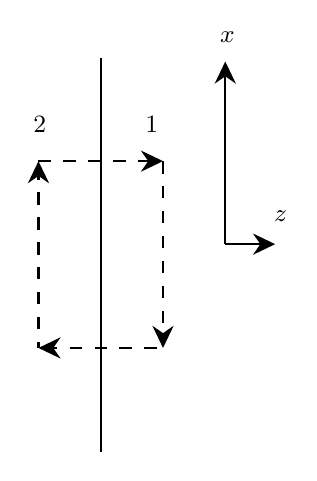
\begin{tikzpicture}[x=0.75pt,y=0.75pt,yscale=-1,xscale=1]
%uncomment if require: \path (0,300); %set diagram left start at 0, and has height of 300

%Straight Lines [id:da6688995942279288] 
\draw    (220,40.36) -- (220,230.36) ;
%Straight Lines [id:da8581026792782027] 
\draw  [dash pattern={on 4.5pt off 4.5pt}]  (250,90.2) -- (250,177.2) ;
\draw [shift={(250,180.2)}, rotate = 270] [fill={rgb, 255:red, 0; green, 0; blue, 0 }  ][line width=0.08]  [draw opacity=0] (10.72,-5.15) -- (0,0) -- (10.72,5.15) -- (7.12,0) -- cycle    ;
%Straight Lines [id:da6765706379121441] 
\draw  [dash pattern={on 4.5pt off 4.5pt}]  (190,93.2) -- (190,180.2) ;
\draw [shift={(190,90.2)}, rotate = 90] [fill={rgb, 255:red, 0; green, 0; blue, 0 }  ][line width=0.08]  [draw opacity=0] (10.72,-5.15) -- (0,0) -- (10.72,5.15) -- (7.12,0) -- cycle    ;
%Straight Lines [id:da1507804766416887] 
\draw  [dash pattern={on 4.5pt off 4.5pt}]  (193,180.2) -- (203.02,180.2) -- (250,180.2) ;
\draw [shift={(190,180.2)}, rotate = 0] [fill={rgb, 255:red, 0; green, 0; blue, 0 }  ][line width=0.08]  [draw opacity=0] (10.72,-5.15) -- (0,0) -- (10.72,5.15) -- (7.12,0) -- cycle    ;
%Straight Lines [id:da47356020778772123] 
\draw  [dash pattern={on 4.5pt off 4.5pt}]  (190,90.2) -- (247,90.2) ;
\draw [shift={(250,90.2)}, rotate = 180] [fill={rgb, 255:red, 0; green, 0; blue, 0 }  ][line width=0.08]  [draw opacity=0] (10.72,-5.15) -- (0,0) -- (10.72,5.15) -- (7.12,0) -- cycle    ;
%Straight Lines [id:da18579905489258697] 
\draw    (280,45.2) -- (280,130.2) ;
\draw [shift={(280,42.2)}, rotate = 90] [fill={rgb, 255:red, 0; green, 0; blue, 0 }  ][line width=0.08]  [draw opacity=0] (10.72,-5.15) -- (0,0) -- (10.72,5.15) -- (7.12,0) -- cycle    ;
%Straight Lines [id:da8596726109827932] 
\draw    (301.02,130.2) -- (280,130.2) ;
\draw [shift={(304.02,130.2)}, rotate = 180] [fill={rgb, 255:red, 0; green, 0; blue, 0 }  ][line width=0.08]  [draw opacity=0] (10.72,-5.15) -- (0,0) -- (10.72,5.15) -- (7.12,0) -- cycle    ;

% Text Node
\draw (240,67.4) node [anchor=north west][inner sep=0.75pt]  [font=\small]  {$1$};
% Text Node
\draw (186,67.4) node [anchor=north west][inner sep=0.75pt]  [font=\small]  {$2$};
% Text Node
\draw (276,26.4) node [anchor=north west][inner sep=0.75pt]  [font=\small]  {$x$};
% Text Node
\draw (302,112.4) node [anchor=north west][inner sep=0.75pt]  [font=\small]  {$z$};


\end{tikzpicture}
        \end{center}
        \begin{align*}
            \ot{B_1^{\parallel}}&=\dfrac{g_2}{x^2}\ot{x_0}=-\dfrac{g_1}{x^2}\ot{x_0}.\\
            \ot{B_2^{\parallel}}&=\dfrac{g_1}{x^2}\ot{x_0}.
        \end{align*}
        Đối với một vòng vuông góc với trục $X$ và dọc theo trục $Y$ (hướng ra ngoài mặt phẳng tờ giấy). Tích phân trên đường cong kín
        \[\oint_{\ell}\ot{B}\mathrm{d}\ot{\ell}=\ot{B_1^{\parallel}}\cdot L\ot{y_0}-\ot{B_2^\parallel}\cdot L\ot{y_0}=0-0=0.\]
        Đối với một vòng song song với trục $X$ như hình vẽ ta có
        \[\oint_{\ell}\ot{B}\mathrm{d}\ot{\ell}=-\ot{B_1^{\parallel}}\cdot L\ot{x_0}+\ot{B_2^{\parallel}}\cdot L \ot{x_0}=\dfrac{Lg_1}{x^2}+\dfrac{Lg_1}{x^2}=\dfrac{2Lg_1}{x^2}.\]
        Gọi mật độ dòng điện mặt là $K$, khi đó 
        \[\dfrac{2Lg_1}{x^2}=\oint_{\ell}\ot{B}\mathrm{d}\ot{\ell}=4\pi KL.\]
        Sử dụng quy tắc bàn tay phải ta có $\ot{K}=-\dfrac{g_1}{2\pi x^2}\ot{y_0}.$ 
        Vector này hướng vuông góc vào mặt tờ giấy. Nói chung ta có
        \[\ot{K}=\dfrac{g_1}{2\pi}\dfrac{(y\ot{x_0}-x\ot{y_0})}{(x^2+y^2)^{\frac{3}{2}}}.\]
        Có vài cách khác để dẫn tới kết quả trên đối với mật độ dòng điện đều là tốt.
    \end{enumerate}
\end{enumerate}
\end{loigiai}


\begin{vd}[Bi-a từ tính]
 Xét hai quả cầu điện môi đàn hồi tuyệt đối bán kính $r$ và khối lượng $m$, một quả cầu mang điện tích phân bố đẳng hướng $-q$ và quả cầu kia mang điện tích $+q$. Có từ trường đều $B$ song song với trục $Oz$ đủ mạnh để có thể bỏ qua tương tác tĩnh điện của hai điện tích, bỏ qua trọng lực và lực ma sát.
 \\Quả cầu thứ nhất (tích điện âm) chuyển động với vận tốc $v$ và va chạm với quả cầu thứ hai đang nằm yên ở gốc tọa độ. Va chạm là xuyên tâm, và ngay trước khi va chạm, vận tốc của quả cầu thứ nhất song song với trục $Ox$.
 \begin{enumerate}[1)]
     \item Vận tốc của quả cầu thứ hai ngay sau va chạm là bao nhiêu?
     \item Vẽ các quỹ đạo của các trọng tâm của cả hai quả bóng trong quá trình chuyển động sau đó.
     \item Vận tốc trung bình (độ lớn và hướng) của các quả cầu trong quá trình chuyển động sau đó của chúng là bao nhiêu?
 \end{enumerate}
\end{vd}
\begin{loigiai}
\begin{enumerate}[1)]
    \item Gọi vận tốc sau va chạm của hai quả bóng tương ứng là $v_1$, $v_2$. Áp dụng định luật bảo toàn năng lượng:
    $$\dfrac{mv^2}{2}=\dfrac{mv_1^2}{2}+\dfrac{mv_2^2}{2},$$
    hay
    $$v^2=v_1^2+v_2^2.$$
    Áp dụng định luật bảo toàn động lượng:
    $$mv=mv_1+mv_2,$$
    hay 
    $$v=v_1+v_2.$$
    Từ hai phương trình trên ta có: 
    $$v^2=v_2^2+(v-v_2)^2=v^2-2vv_2+v_2^2.$$
    \[ \Rightarrow \left[ \begin{gathered}
      {v_2} = 0 \hfill \\
      {v_2} = v \hfill \\ 
    \end{gathered}  \right.\]
    \item Các quả bóng chịu lực Lorentz do từ trường. Vì lực Lorentz có phương vuông góc với đường chuyển động và có độ lớn không đổi nên các quả cầu chuyển động theo quỹ đạo tròn. Lực Lorentz đóng vai trò là lực hướng tâm: 
    $$m\dfrac{v^2}{R}=qvB.$$
    Với bán kính quỹ đạo $$R=\dfrac{mv}{qB}$$
    và tốc độ góc $$\omega=\dfrac{v}{R}=\dfrac{qB}{m}.$$
    Do đó một trong các điện tích di chuyển dọc theo quỹ đạo tròn theo chiều kim đồng hồ và điện tích kia ngược chiều kim đồng hồ.
    \\Sau mỗi lần va chạm, một trong hai quả cầu chuyển động với vận tốc $v$ trong khi quả cầu kia đứng yên. Quả cầu chuyển động đi một phần của chu kì cyclotron đầy đủ (chiều chuyển động phụ thuộc vào dấu điện tích) trước khi va chạm xuyên tâm với quả cầu đang dừng. Động lượng được truyền cho quả cầu còn lại và quả cầu chuyển động trước đó lại đứng yên và chu kì đó lặp đi lặp lại. Trong những lần va chạm tiếp theo, các quả cầu bắt đầu trôi theo một hướng như trong hình.
    \begin{center}
        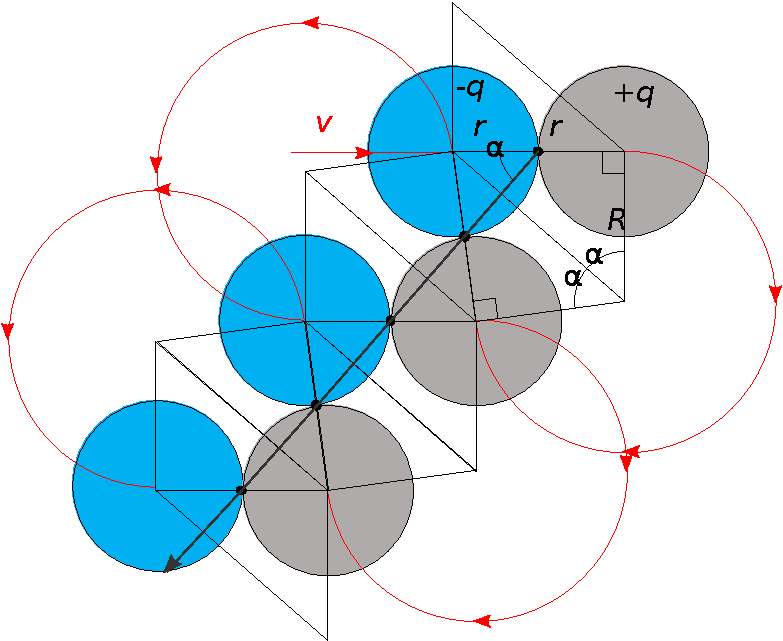
\includegraphics[scale=0.75]{Anh/Trung1.pdf}
    \end{center}
    \item Vận tốc trung bình của các quả cầu bằng vận tốc trung bình của các điểm va chạm. Từ hình vẽ, có thể thấy rằng hướng của vận tốc trung bình là $\pi-\alpha$ theo chiều kim đồng hồ tính từ hướng ban đầu của quả cầu tới, ta có: $$\alpha=\arctan{\dfrac{2r}{R}}.$$
    Độ dịch chuyển của điểm va chạm giữa hai lần là:
    $$d=rcos\alpha.$$
    Giữa hai lần va chạm, quả cầu di chuyển một góc $2\pi-2\alpha$ trên quỹ đạo tròn, do đó thời gian giữa hai lần va chạm là:
    $$t=\dfrac{2\pi-2\alpha}{\omega}=\dfrac{2m}{qB}\left(\pi-\arctan{\dfrac{2r}{R}}\right).$$
    Từ đó ta tính được vận tốc trung bình:
    $$v_{\mathrm{avg}}=\dfrac{d}{t}=\dfrac{r\omega\cos\alpha}{2(\pi-\alpha)}=\dfrac{vrR}{R\sqrt{4r^2+R^2}(\pi-\alpha)}=\dfrac{v}{\sqrt{4+\dfrac{R^2}{r^2}}\left(\pi-\arctan{\dfrac{2r}{R}}\right)}.$$
\end{enumerate}
\end{loigiai}

\begin{vd}[Cáp truyền tín hiệu]
    Một cáp truyền tín hiệu đối xứng trục được cấu tạo từ một lõi hình trụ bên trong bán kính $a=2\dv{cm}$ và một vỏ trụ bên ngoài đồng trục bán kính trong $b=5\dv{cm}$ và bán kính ngoài $c=7\dv{cm}$. Một dòng điện có độ lớn $I=5\dv{A}$ phân bố đều chạy trong lõi và một dòng điện khác cùng độ lớn, phân bố đều nhưng ngược chiều chạy trong vỏ ngoài. Tìm cảm ứng từ $B$ tại điểm cách trục cáp $r$.\\ 
    Tính $\displaystyle\int^\infty_0B(r)\mathrm{d}r$. 
\end{vd}
\begin{loigiai}
    Sử dụng định luật Ampere
    $$ \oint \ot{B} \cdot \ot{\mathrm{d}l}= \mu_0I.$$
    Ta thu được 
    $$ B(r)=\dfrac{\mu_0I(r)}{2\pi r}.$$
    \begin{itemize}
        \item[$*)$] Khi $r<a:$ $$ B(r)=\dfrac{\mu_0Ir}{2\pi a^2}. $$
        \item[$*)$] Khi $a\leq r<b:$  $$B(r)=\dfrac{\mu_0I}{2\pi r}.$$
        \item[$*)$] Khi $b\leq r<c:$  $$B(r)=\dfrac{\mu_0I}{2\pi}\left(\dfrac{c^2}{r(c^2-b^2)}-\dfrac{r}{c^2-b^2}\right).$$
        \item[$*)$] Khi $r\geq c:$ $$B(r)=0.$$
    \end{itemize}
    Suy ra: 
    \begin{equation*}
        \begin{aligned}
            \int_0^\infty B(r)\mathrm{d}r &= \int_0^a\dfrac{\mu_0Ir}{2\pi a^2}\mathrm{d}r + \int_a^b\dfrac{\mu_0I}{2\pi r}\mathrm{d}r + \int_b^c\dfrac{\mu_0I}{2\pi}\left(\dfrac{c^2}{r(c^2-b^2)} - \dfrac{r}{c^2-b^2}\right)\mathrm{d}r\\
            &= \dfrac{\mu_0I}{2\pi}\left[\left.\left(\dfrac{r^2}{2a^2}\right) \right|_0^a + \left. \ln{r}\right|_a^b + \left.\left(\dfrac{c^2}{c^2-b^2}\ln{r}\right)\right|_b^c - \left.\dfrac{r^2}{2(c^2-b^2)}\right|_b^c \ \right].
        \end{aligned}
    \end{equation*}
    Thay số ta được
    $$\int_0^\infty B(r)\mathrm{d}r = 1.6\times10^{-6}\dv{T}.\dv{m}$$
    \end{loigiai}


\begin{vd}[Vòng siêu dẫn]
    Xét một vòng hình chữ nhật làm từ vật liệu siêu dẫn dài $l=200\dv{cm}$ và rộng $w=2\dv{cm}$. Bán kính của dây là $r=0.5\dv{mm}$. Ban đầu vòng dây có dòng điện $I_1=5\dv{A}$. Cách vòng $d=1\dv{cm}$ có một dây dẫn dài vô hạn không có dòng điện. Dòng điện trong dây dẫn tăng đến $I_2$ sao cho có một lực hút $F$ giữa vòng và dây. Tìm giá trị lớn nhất có thể của $F$.
    \begin{center}
        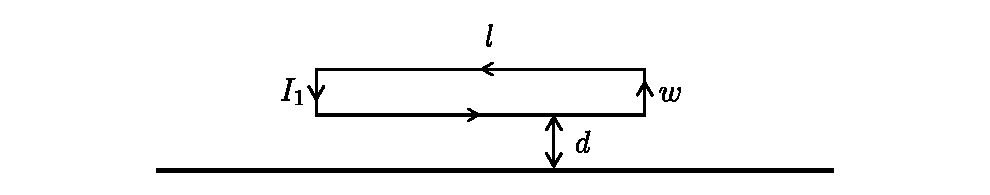
\includegraphics[width=\textwidth]{Anh/15.pdf}
    \end{center}
\end{vd}
\begin{loigiai}
Từ thông qua vòng dây siêu dẫn phải có giá trị không đổi. Nếu không, sự biến thiên từ thông qua vòng dây sẽ gây ra trên vòng dây một suất điện động
$$\varepsilon=\dfrac{\dd\phi}{\dd t}.$$
Mà vòng dây siêu dẫn lại có điện trở bằng không, điều này dẫn đến là dòng điện trong dây tiến đến vô cùng. Điều này là vô lí.\\
Đầu tiên ta sẽ tính từ thông qua vòng khi mà dòng điện trong vòng là $I_1$. Ta thấy là $ư\ll l$, nên ta có thể bỏ qua từ thông gây ra bởi các cạnh ngắn của vòng dây. Ngoài ra, ta còn có thể coi là từ trường gây ra bởi cạnh dài như là từ trường gây ra bởi dây dẫn dài vô hạn $B=\dfrac{\mu_0I}{2\pi r}$.\\
Từ thông qua vòng dây  
\begin{equation*}
    \begin{aligned}
     \phi_1&=\tiph{r}{w-r}{B(r)l}{r'}\\
     &=\tiph{r}{w-r}{\tron{\dfrac{\mu_0I_1l}{2\pi r'} + \dfrac{\mu_0I_1l}{2\pi \tron{w-r'}}}}{r'}\\
     &=\dfrac{\mu_0I_1l}{\pi}\ln\tron{\dfrac{w}{r}}.
    \end{aligned}
\end{equation*}
Độ tự cảm của vòng dây là $L=\dfrac{\phi_1}{I_1}=\dfrac{\mu_0l}{\pi}\ln\tron{\dfrac{w}{r}}$.\\
Bây giờ ta tính từ thông do dây dẫn gửi qua vòng dây.
\begin{equation*}
    \begin{aligned}
     \phi_2&=\tiph{d}{d+w}{\dfrac{mu_0I_2l}{2\pi r'}}{r'}\\
     &=\dfrac{\mu_0I_2l}{2\pi}\ln\tron{\dfrac{d+w}{d}}.
    \end{aligned}
\end{equation*}
Độ hỗ cảm của vòng dây và dây dẫn là $M=\dfrac{\phi_2}{I_2}=\dfrac{\mu_0l}{2\pi}\ln\tron{\dfrac{d+w}{d}}$.\\
Khi có dòng $I_2$ chạy trong dây dẫn, dòng điện trong vòng là $I_3$. Ta có
\begin{equation*}
    \begin{aligned}
     &LI_1=MI_2+LI_3\\
     \Leftrightarrow & I_3=I_1-\dfrac{MI_2}{L}.
    \end{aligned}
\end{equation*}
Lực tác dụng lên vòng dây
\begin{equation*}
    \begin{aligned}
     F&=I_3l\tron{\dfrac{\mu_0I_2}{2\pi d}-\dfrac{\mu_0I_2}{2\pi(d+w)}}\\
     &=\dfrac{\mu_0lư}{2\pi(d+w)d}\tron{I_1I_2-
    \dfrac{M{I_2}^2}{L}}.
    \end{aligned}
\end{equation*}
Giá trị của $F$ cực đại khi $I_2=\dfrac{I_1L}{2M}$, thay số vào ta tính được
$$F_{max}=1.12\times10^{-13}\dv{N}.$$
\end{loigiai}

\begin{vd}[Gió Mặt Trời]
 Các hạt có khối lượng $m$ và điện tích $q$ được phóng từ gốc tọa độ với vận tốc $v$ song song với trục $\mathrm{O}x$. Có màn chắn tại $x=\ell$.
    \begin{enumerate}[1)]
    \item Hạt thứ nhất được phóng ra khi có điện trường đều song song với trục $x$ và không có từ trường. Cường độ điện trường phải bằng bao nhiêu để hạt không bao giờ tới được màn?
    \item Tiếp theo, điện trường bị tắt, một từ trường đều hướng theo trục $\mathrm{O}z$ trong vùng $0<x<\ell$ được bật lên và hạt thứ hai được phóng ra. Biết rằng tốc độ của hạt vừa đủ lớn để tới màn chắn, hãy phác thảo quỹ đạo và tìm cường độ từ trường $B$.
    \item Cuối cùng, một điện trường $E$ nằm trong mặt phẳng $\mathrm{Oxy}$ được bật trong khi $B$ không đổi. Hạt thứ ba được bắn ra từ điểm gốc, vẫn song song với trục $\mathrm{O}x$, nhưng có thể với tốc độ khác. Người ta quan sát thấy rằng hạt chuyển động không bị lệch. Và thời gian cần thiết để nó tới màn chắn giống như đối với hạt thứ hai. Tìm độ lớn của điện trường $E$.
    \item Bỏ qua các ý trước, bây giờ chúng ta nghiên cứu một từ trường yếu không đều: các đường sức từ có bán kính cong lớn hơn nhiều bán kính cong của quỹ đạo hạt. Dường như trong trường hợp này, bất biến đoạn nhiệt của một hạt trong từ trường được bảo toàn: từ thông bao quanh quỹ đạo hình xoắn của hạt không đổi với độ chính xác cao dọc theo quỹ đạo. 
    \\Hãy xem xét một mô hình rất đơn giản về cách các hạt gió Mặt trời tương tác với từ trường của Trái Đất. Cường độ của từ trường Trái Đất trên trục từ của nó có thể được biểu thị bằng $B_z=B_E(R_E/z)^3$, trong đó $B_E = 3,12.10^{-5}~\mathrm{T}$ là cường độ trường tại bề mặt Trái Đất tại cực từ, $R_E = 6370 \mathrm{km}$ là bán kính Trái Đất và $z$ được đo từ tâm Trái Đất.
    \\Một electron mang điện tích $ -e = -1,60.10^{-19} \mathrm{C}$ và khối lượng $m_e = 9,11.10^{-31}~ \mathrm{kg}$ đang đến gần Trái Đất với vận tốc $u_0 = 500 ~\mathrm{km/s}$ và đập vào từ trường Trái Đất ngay trên trục của nó với một góc $\alpha$ ở khoảng cách $R_0 = 5R_E$ và bắt đầu xoắn ốc về phía Trái Đất. Nếu $\alpha$ quá lớn, hạt sẽ bị phản xạ bởi cường độ từ trường tăng dần khi hạt đến gần Trái Đất. Tìm điều kiện của $\alpha$ để hạt tới được bề mặt Trái Đất. 
    \\Có thể bỏ qua các hiệu ứng hấp dẫn hoặc tương đối tính. 
    \end{enumerate}
\end{vd}
\begin{loigiai}
\begin{enumerate}[1)]
    \item Trong điện trường đều $E$ dọc theo trục $\mathrm{O}x$, ta có điện thế
    \[\Phi(x)=-xE.\]
    Để hạt không va vào tường, động năng $\dfrac{mv^2}{2}$ của hạt phải nhỏ hơn công của lực điện $q\Phi(\ell)=-q\ell E$.
    \\ Do đó 
    \[\left|E\right| >\dfrac{mv^2}{2\ell \left|q\right|}.\]
     Và hướng của $E$ thỏa mãn $qE<0$.
    \item Trong từ trường, hạt chuyển động theo quỹ đạo đường tròn bán kính $R$, khi đó lực Lorentz đóng vai trò là lực hướng tâm: \[qvB=\dfrac{mv^2}{R}.\]
    Để hạt vừa đủ chạm vào màn thì quỹ đạo tròn phải tiếp xúc với màn.
    \\ Vì vậy $R=\ell$ và $B=\dfrac{mv}{q\ell}$.
    \begin{center}
        \tikzset{every picture/.style={line width=0.75pt}} %set default line width to 0.75pt        
        
        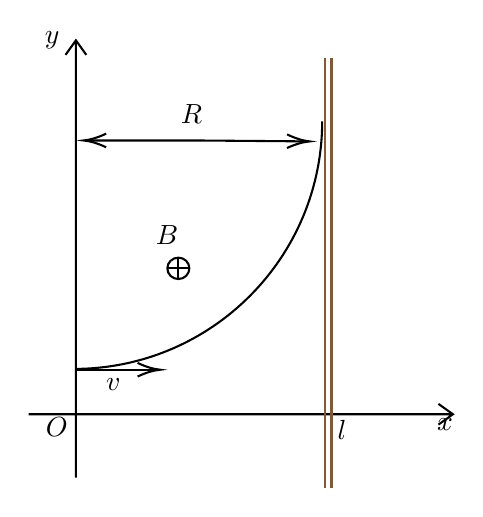
\begin{tikzpicture}[x=0.75pt,y=0.75pt,yscale=-1,xscale=1]
        %uncomment if require: \path (0,470); %set diagram left start at 0, and has height of 470
        
        %Shape: Axis 2D [id:dp9892750012986586] 
        \draw  (234.21,331.85) -- (438.6,331.85)(256.95,151.7) -- (256.95,362.4) (431.6,326.85) -- (438.6,331.85) -- (431.6,336.85) (251.95,158.7) -- (256.95,151.7) -- (261.95,158.7)  ;
        %Shape: Arc [id:dp1911045005650318] 
        \draw  [draw opacity=0] (256.7,310) .. controls (322.39,309.65) and (375.54,256.38) .. (375.6,190.7) -- (256.05,190.6) -- cycle ; \draw   (256.7,310) .. controls (322.39,309.65) and (375.54,256.38) .. (375.6,190.7) ;
        %Straight Lines [id:da1899490342711958] 
        \draw [color={rgb, 255:red, 139; green, 87; blue, 42 }  ,draw opacity=1 ][fill={rgb, 255:red, 74; green, 144; blue, 226 }  ,fill opacity=1 ]   (380.1,160.4) -- (380.1,260.2) -- (380.1,367.4)(377.1,160.4) -- (377.1,260.2) -- (377.1,367.4) ;
        %Flowchart: Or [id:dp8098590146376892] 
        \draw   (301,261.55) .. controls (301,258.71) and (303.37,256.4) .. (306.3,256.4) .. controls (309.23,256.4) and (311.6,258.71) .. (311.6,261.55) .. controls (311.6,264.39) and (309.23,266.7) .. (306.3,266.7) .. controls (303.37,266.7) and (301,264.39) .. (301,261.55) -- cycle ; \draw   (301,261.55) -- (311.6,261.55) ; \draw   (306.3,256.4) -- (306.3,266.7) ;
        %Straight Lines [id:da774970081443114] 
        \draw    (257.2,310.4) -- (295.6,310.4) ;
        \draw [shift={(297.6,310.4)}, rotate = 180] [color={rgb, 255:red, 0; green, 0; blue, 0 }  ][line width=0.75]    (10.93,-3.29) .. controls (6.95,-1.4) and (3.31,-0.3) .. (0,0) .. controls (3.31,0.3) and (6.95,1.4) .. (10.93,3.29)   ;
        %Straight Lines [id:da13664569510303481] 
        \draw    (262.6,199.94) -- (314.6,199.94) -- (367.6,200.38) ;
        \draw [shift={(369.6,200.4)}, rotate = 180.48] [color={rgb, 255:red, 0; green, 0; blue, 0 }  ][line width=0.75]    (10.93,-3.29) .. controls (6.95,-1.4) and (3.31,-0.3) .. (0,0) .. controls (3.31,0.3) and (6.95,1.4) .. (10.93,3.29)   ;
        \draw [shift={(260.6,199.94)}, rotate = 0] [color={rgb, 255:red, 0; green, 0; blue, 0 }  ][line width=0.75]    (10.93,-3.29) .. controls (6.95,-1.4) and (3.31,-0.3) .. (0,0) .. controls (3.31,0.3) and (6.95,1.4) .. (10.93,3.29)   ;
        
        
        % Text Node
        \draw (381.5,333.1) node [anchor=north west][inner sep=0.75pt]    {$l$};
        % Text Node
        \draw (241,332.1) node [anchor=north west][inner sep=0.75pt]    {$O$};
        % Text Node
        \draw (429.5,332.6) node [anchor=north west][inner sep=0.75pt]    {$x$};
        % Text Node
        \draw (240.5,146.1) node [anchor=north west][inner sep=0.75pt]    {$y$};
        % Text Node
        \draw (294,239.4) node [anchor=north west][inner sep=0.75pt]    {$B$};
        % Text Node
        \draw (270,313.4) node [anchor=north west][inner sep=0.75pt]    {$\ot{v}$};
        % Text Node
        \draw (306,181.4) node [anchor=north west][inner sep=0.75pt]    {$R$};
        
        
        \end{tikzpicture}
    \end{center}
    \item Thời gian cần thiết để hạt thứ 2 tới màn chắn là \[t=\dfrac{T}{4}=\dfrac{\pi l}{2v}.\]
    \\Để hạt chuyển động không bị lệch thì lực điện phải cân bằng với lực từ:
    $$F_E=F_B$$
    $$\rt qE=quB$$
    $$\rt u=\dfrac{E}{B}$$
    Vì thời gian cần thiết để hạt thứ 3 tới màn chắn giống hạt thứ 2 nên ta có: 
    $$t=\dfrac{l}{u}=\dfrac{\pi l}{2v}$$
    $$\rt E=\dfrac{2vB}{\pi}$$
    \item Ta có từ thông $\Phi \sim \text{Diện tích} \times B_z \sim R^2 B_z \sim \dfrac{B_z}{v_ \bot ^2} $, trong đó $v_\bot$ là thành phần vận tốc vuông góc với từ trường. Mà từ thông $\Phi$ là một đại lượng bất biến nên $\dfrac{B_z}{v_ \bot ^2}$ cũng là một bất biến.
    \\Trong quá trình chuyển động của electron, động năng của nó được bảo toàn vì từ trường không thực hiện công.
    \\Trong trường hợp tới hạn, khi electron gần như bị phản xạ, thành phần vận tốc vuông góc của electron ở bề mặt Trái Đất sẽ bằng $u_0$. Khi đó, bất biến đoạn nhiệt sẽ cho kết quả:
    \[\dfrac{{v_{ \bot 0}^2}}{{B\left( {{R_0}} \right)}} = \dfrac{{u_0^2}}{{B\left( {{R_E}} \right)}}\]
    Với ${v_{ \bot 0}} = {u_0}\sin \alpha$, ta có:
    \[{\alpha _0} = \arcsin \left( {\sqrt {\dfrac{{B\left( {{R_0}} \right)}}{{B\left( {{R_E}} \right)}}} } \right) = \arcsin \left( {\dfrac{1}{{5\sqrt 5 }}} \right) = 5,13^\circ \]
    Góc $\alpha$ cần nhỏ hơn $\alpha_0$ để electron có thể tới được bề mặt Trái Đất.
\end{enumerate}
\end{loigiai}

\begin{vd}[Hệ spin]
    Chúng ta hãy xem xét một hệ thống gồm $N$ lưỡng cực từ độc lập (spins) trong từ trường $B$ và nhiệt độ $T$. Mục tiêu là xác định một số tính chất của hệ này bằng cách sử dụng vật lí thống kê. Biết rằng năng lượng của một spin đơn là $E=\epsilon m$, trong đó $m=\pm \dfrac{1}{2}$ và $\epsilon=\alpha B$.
    \begin{enumerate}[1)]
        \item Xác suất $p_\uparrow$ để một spin ở trạng thái kích thích, tức là có năng lượng dương?
        \item Giá trị trung bình của tổng năng lượng $E_s$ của hệ spin là một hàm của $B$ và $T$ ?
        \item  Sử dụng phương pháp xấp xỉ nhiệt độ cao $T \gg \dfrac{\alpha Bm}{k}$, đơn giản hóa biểu thức của $E_s$.
        \item Sử dụng phương pháp xấp xỉ nhiệt độ cao $T \gg \dfrac{\alpha Bm}{k}$, đơn giản hóa biểu thức của $E_s$. Tìm nhiệt dung C của hệ spin.
    \end{enumerate}
\end{vd}

\begin{loigiai}
    \begin{enumerate}[1)]
        \item Theo phân bố Boltzmann, $p_\uparrow=A\dot e^{-\epsilon m}$.
        \\ Trong đó hằng số $A$ có thể tìm được với điều kiện tổng xác suất spin quay lên hoặc xuống là $1$:
        \[A = \frac{1}{{{e^{ - \epsilon /2kT}}} + {e^{\epsilon /2kT}}} = \frac{1}{{2\cosh \left( {\epsilon /2kT} \right)}}.\]
        Do đó 
        \[{p_ \uparrow } = \dfrac{{{e^{-\epsilon/2kT} }}}{{{e^{-\epsilon/2kT}} + {e^{\epsilon/2kT}}}}\]
        \item Năng lượng trung bình là giá trị trung bình có trọng số của năng lượng trạng thái lên và xuống cho một lần quay, nhân với số lần quay:
        \[E = \frac{{N\epsilon }}{2}\frac{{{e^{ - \epsilon /2kT}} - {e^{\epsilon /2kT}}}}{{{e^{ - \epsilon /2kT}}{ + e^{\epsilon /2kT}}}} =  - \frac{{N\epsilon }}{2}\tanh \left( {\epsilon /2kT} \right).\]
        \item Đối với các giá trị đối số nhỏ của tiếp tuyến hyperbol, biểu thức có thể tính gần đúng:
        \[E \approx \frac{{ - N{\epsilon ^2}}}{{4kT}}.\]
        \item Theo định nghĩa của nhiệt dung:
        \[C = \dfrac{\mathrm{d}E}{\mathrm{d}t} = \frac{{N{\epsilon ^2}}}{{4k{T^2}}}.\]
    \end{enumerate}
\end{loigiai}

\begin{vd}[Nối hai solenoid]
    Một cuộn dây Solenoid cứng quấn chặt được lắp một phần vào một cuộn dây khác. Chúng được nối với một nguồn điện không đổi; cả hai đều tạo ra một từ trường cùng hướng. Cả hai đều có $N$ vòng xoắn, chiều dài của chúng là $l$, diện tích mặt cắt ngang của chúng là $A_1$ và $A_2$. Có thể giả định rằng $A_1, A_2 \ll l^2$.
    \\Biết rằng từ trường tại tâm của một Solenoid được lấy riêng là $B =\dfrac{\mu_0 IN}{l}$, trong đó $\mu_0$ là độ từ thẩm của chân không.
    \begin{enumerate}[1)]
        \item Tâm của các cuộn dây cách nhau một khoảng $x<l$ dọc theo trục chung của chúng $\left[A_1, A_2 \ll (x-l)^2, x^2\right]$. Tìm tổng năng lượng $E_m$ của từ trường trong hệ.
        \item Tìm suất điện động $\varepsilon_1$ và $\varepsilon_2$ sinh ra trên cuộn dây khi người ta kéo ra với tốc độ $v$.
        \item Tìm lực $F$ cần thiết để kéo một cuộn dây ra phía ngoài.
    \end{enumerate}
\end{vd}

\begin{loigiai}
    \begin{enumerate}[1)]
        \item Vùng chồng chập 2 cuộn dây có từ trường $2B$, phần còn lại của cuộn dây bên trong có từ trường $B$. Cho cuộn dây bên trong có diện tích $A_2$. Mật độ năng lượng của phần cuộn dây bên trong có từ trường $B$ là $\dfrac{B^2}{2 \mu_0}$. 
    \\Do đó năng lượng của từ trường trong hệ 2 cuộn dây là
    \[\begin{aligned}
            E_m &=\dfrac{B^2}{2\mu_0}\left(A_1l-A_2(l-x)+A_2x \right)+\dfrac{(2B)^2}{2\mu_0}A_2(l-x) \\
            &=\dfrac{B^2}{2\mu_0}\left[ A_1l+A_2(3l-2x)\right]\\
               &=\dfrac{\mu_0 I^2 N^2}{2l^2}\left[A_1l+A_2(3l-2x)\right].
    \end{aligned}\]
    \item Tiết diện $A_1$ của cuộn dây bên ngoài được cắt bởi tất cả từ thông $ B\cdot A_2$ của cuộn dây bên trong. Sau thời gian $\dd t$, từ thông này được được bao bọc bởi ít vòng của cuộn dây bên ngoài hơn $-$ bởi $\dfrac{Nv \mathrm{d}t}{l}$ vòng dây có chiều dài $v \mathrm{d}t$. Do đó từ thông được bao bởi cuộn dây bên ngoài thay đổi với tốc độ 
    \[\varepsilon_1 = \dot \Phi_1=\dfrac{BA_2Nv}{l}=\dfrac{\mu_0A_2IN^2v}{l^2}.\]
    Cuộn dây bên trong cũng được cắt bởi từ thông $BA_2$, do đó $\varepsilon_2=\varepsilon_1$ và cùng chiều.
    \item Ta thấy năng lượng từ trường giảm và nguồn dòng điện không đổi bị tiêu tán một phần năng lượng (vì suất điện động cảm ứng có chiều ngược lại nguồn điện).
    \\ Theo định luật bảo toàn năng lượng, ta có công để kéo cuộn dây ra là:
    \[Fv=\dfrac{\mathrm{d}E_m}{\mathrm{d}x}v+I(\varepsilon_1+\varepsilon_2).\]
    Từ đó ta tính được 
    \[F=-\dfrac{B^2A_2}{\mu_0}+\dfrac{2IBA_2N}{l}=\dfrac{\mu_0I^2N^2A_2}{l^2}.\]
    \end{enumerate}
\end{loigiai}

\begin{vd}[Cyclotron]
Ta xét một cyclotron (một loại máy gia tốc hạt nhất) và hoạt động của nó. Cyclotron bao gồm một vùng hình trụ bán kính $R$ nơi có từ trường đều có cảm ứng từ $B$ và một vùng hình dải mỏng có chiều rộng $d$ tại đó có điện trường đều cường độ $E$ vuông góc với dải. Hướng của điện trường được thay đổi tuần hoàn thành hướng ngược lại sao cho mọi hạt đi qua dải, hướng của điện trường giống với hướng của vận tốc của hạt. Cũng có một kênh hẹp ở một cạnh của cyclotron để các hạt thoát ra khỏi cyclotron. Cho các hạt bắt đầu chuyển động ở tâm của xiclôtron với tốc độ ban đầu nhỏ không đáng kể.
\\Trước khi rời khỏi cyclotron, hạt sẽ đi được $n$ vòng tròn đủ, tìm $n$.
\\ Cho điện tích của các hạt là $q$ và khối lượng $m$.
\\Và giả sử rằng $n\gg1$.
\begin{center}
    

\tikzset{every picture/.style={line width=0.75pt}} %set default line width to 0.75pt        

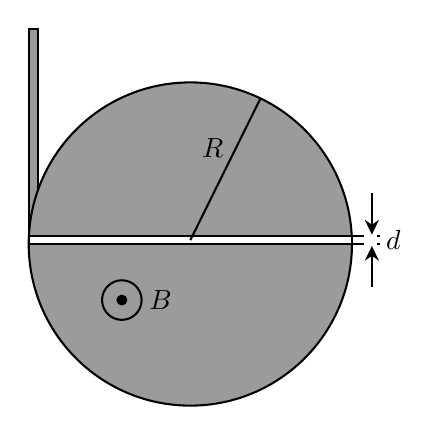
\begin{tikzpicture}[x=0.5pt,y=0.5pt,yscale=-1,xscale=1]
%uncomment if require: \path (0,424); %set diagram left start at 0, and has height of 424

%Shape: Rectangle [id:dp5625641528781005] 
\draw  [fill={rgb, 255:red, 155; green, 155; blue, 155 }  ,fill opacity=1 ] (181,43.2) -- (181,193.2) -- (174,193.2) -- (174,43.2) -- cycle ;
%Shape: Circle [id:dp42258690714876335] 
\draw  [fill={rgb, 255:red, 155; green, 155; blue, 155 }  ,fill opacity=1 ] (174,198.8) .. controls (174,134.29) and (226.29,82) .. (290.8,82) .. controls (355.31,82) and (407.6,134.29) .. (407.6,198.8) .. controls (407.6,263.31) and (355.31,315.6) .. (290.8,315.6) .. controls (226.29,315.6) and (174,263.31) .. (174,198.8) -- cycle ;
%Shape: Rectangle [id:dp6859026345150396] 
\draw  [fill={rgb, 255:red, 255; green, 255; blue, 255 }  ,fill opacity=1 ] (174,193.2) -- (407.6,193.2) -- (407.6,198.8) -- (174,198.8) -- cycle ;
%Straight Lines [id:da6880432905637432] 
\draw    (341.6,93.4) -- (290.8,196) ;
%Straight Lines [id:da023630750235380305] 
\draw  [dash pattern={on 4.5pt off 4.5pt}]  (407.6,193.2) -- (427.6,193.2) ;
%Straight Lines [id:da29515349754415054] 
\draw  [dash pattern={on 4.5pt off 4.5pt}]  (407.6,198.8) -- (427.6,198.8) ;
%Straight Lines [id:da6324336437474667] 
\draw    (422,162.2) -- (422,189) ;
\draw [shift={(422,192)}, rotate = 270] [fill={rgb, 255:red, 0; green, 0; blue, 0 }  ][line width=0.08]  [draw opacity=0] (10.72,-5.15) -- (0,0) -- (10.72,5.15) -- (7.12,0) -- cycle    ;
%Straight Lines [id:da2979405700128157] 
\draw    (422,203.2) -- (422,230) ;
\draw [shift={(422,200.2)}, rotate = 90] [fill={rgb, 255:red, 0; green, 0; blue, 0 }  ][line width=0.08]  [draw opacity=0] (10.72,-5.15) -- (0,0) -- (10.72,5.15) -- (7.12,0) -- cycle    ;
%Shape: Circle [id:dp07336497279632437] 
\draw   (227,239.3) .. controls (227,231.4) and (233.4,225) .. (241.3,225) .. controls (249.2,225) and (255.6,231.4) .. (255.6,239.3) .. controls (255.6,247.2) and (249.2,253.6) .. (241.3,253.6) .. controls (233.4,253.6) and (227,247.2) .. (227,239.3) -- cycle ;
%Shape: Circle [id:dp9231668351446314] 
\draw  [color={rgb, 255:red, 0; green, 0; blue, 0 }  ,draw opacity=1 ][fill={rgb, 255:red, 0; green, 0; blue, 0 }  ,fill opacity=1 ] (238.15,239.3) .. controls (238.15,237.56) and (239.56,236.15) .. (241.3,236.15) .. controls (243.04,236.15) and (244.45,237.56) .. (244.45,239.3) .. controls (244.45,241.04) and (243.04,242.45) .. (241.3,242.45) .. controls (239.56,242.45) and (238.15,241.04) .. (238.15,239.3) -- cycle ;


% Text Node
\draw (430,186.4) node [anchor=north west][inner sep=0.75pt]    {$d$};
% Text Node
\draw (259,230.4) node [anchor=north west][inner sep=0.75pt]    {$B$};
% Text Node
\draw (297,120) node [anchor=north west][inner sep=0.75pt]    {$R$};


\end{tikzpicture}
\end{center}

\end{vd}
\begin{loigiai}\\
Trong cyclotron, các hạt bắt đầu chuyển động theo chiều kim đồng hồ dọc theo một vòng tròn với các nửa vòng liên tục tăng dần. Bán kính quỹ đạo của hạt được tính theo công thức $r=\dfrac{mv}{qB}$,
trong đó $v$ là vận tốc của hạt. Trong một vòng tròn, hạt nhận được động năng $\epsilon_k=2qED$ từ điện trường, vì hạt đi qua dải hai lần trong một vòng tròn. Do đó vận tốc của hạt khi ra khỏi cyclotron là
$$\dfrac{mv^2}{2}=2qEdn$$
$$\rt v^2=\dfrac{4qEdn}{m}.$$
Hạt rời khỏi cyclotron khi bán kính quỹ đạo của nó lớn bằng bán kính $R$ của cyclotron, khi đó, vận tốc của nó là $$v=\dfrac{qBR}{m}.$$
Biểu diễn $n$ từ các phương trình trên ta được $n =\dfrac{ qB^2R^2}{4mEd}$.
\end{loigiai}

\begin{vd}[Ống tia âm cực]%Prob2 IPhO 2000
Một ống tia âm cực (cathode ray tube (CRT)), cấu tạo bởi một súng electron và một màn hình, được dặt trong một từ trường đều, không đổi $\ot{B}$ sao cho từ trườn song song với trục của chùm tia phát ra từ súng như hình vẽ $a)$.
\begin{center}
 

\tikzset{every picture/.style={line width=0.75pt}} %set default line width to 0.75pt        

\begin{tikzpicture}[x=0.75pt,y=0.75pt,yscale=-1,xscale=1]
%uncomment if require: \path (0,652); %set diagram left start at 0, and has height of 652

%Shape: Ellipse [id:dp15688127192695345] 
\draw  [fill={rgb, 255:red, 155; green, 155; blue, 155 }  ,fill opacity=1 ] (333.06,53) .. controls (342.45,53) and (350.07,73.95) .. (350.07,99.79) .. controls (350.07,125.63) and (342.45,146.58) .. (333.06,146.58) .. controls (323.66,146.58) and (316.04,125.63) .. (316.04,99.79) .. controls (316.04,73.95) and (323.66,53) .. (333.06,53) -- cycle ;
%Straight Lines [id:da46382146326331886] 
\draw    (230.82,72.44) -- (333.06,53) ;
%Straight Lines [id:da7484447454061447] 
\draw    (230.82,128.35) -- (333.06,146.58) ;
%Shape: Ellipse [id:dp04390648905852612] 
\draw   (230.82,72.44) .. controls (238.12,72.44) and (244.04,84.96) .. (244.04,100.4) .. controls (244.04,115.83) and (238.12,128.35) .. (230.82,128.35) .. controls (223.52,128.35) and (217.61,115.83) .. (217.61,100.4) .. controls (217.61,84.96) and (223.52,72.44) .. (230.82,72.44) -- cycle ;
%Straight Lines [id:da12460435727279795] 
\draw  [dash pattern={on 4.5pt off 4.5pt}]  (163.38,100.4) -- (483.18,100.4) ;
\draw [shift={(486.18,100.4)}, rotate = 180] [fill={rgb, 255:red, 0; green, 0; blue, 0 }  ][line width=0.08]  [draw opacity=0] (10.72,-5.15) -- (0,0) -- (10.72,5.15) -- (7.12,0) -- cycle    ;
%Rounded Rect [id:dp7059297815675409] 
\draw   (174.86,178.69) .. controls (174.86,170.51) and (181.49,163.87) .. (189.68,163.87) -- (234.16,163.87) .. controls (242.35,163.87) and (248.99,170.51) .. (248.99,178.69) -- (248.99,223.17) .. controls (248.99,231.36) and (242.35,238) .. (234.16,238) -- (189.68,238) .. controls (181.49,238) and (174.86,231.36) .. (174.86,223.17) -- cycle ;
%Straight Lines [id:da6620628016537122] 
\draw    (211.92,200.93) -- (234.41,200.93) -- (501.77,200.93) ;
%Shape: Ellipse [id:dp5076742892764352] 
\draw   (413.66,165.49) .. controls (418.02,165.49) and (421.56,180.72) .. (421.56,199.52) .. controls (421.56,218.31) and (418.02,233.54) .. (413.66,233.54) .. controls (409.3,233.54) and (405.76,218.31) .. (405.76,199.52) .. controls (405.76,180.72) and (409.3,165.49) .. (413.66,165.49) -- cycle ;
%Straight Lines [id:da4821118642858162] 
\draw    (248.38,200.93) -- (413.66,165.49) ;
%Straight Lines [id:da3173684264555092] 
\draw    (248.38,200.93) -- (413.66,233.54) ;
%Straight Lines [id:da7776734544630426] 
\draw    (248.38,200.93) -- (417.91,171.97) ;
%Straight Lines [id:da3980810014347458] 
\draw    (248.38,200.93) -- (406.97,181.69) ;
%Straight Lines [id:da5966138762318254] 
\draw    (249.6,200.93) -- (421.56,187.36) ;
%Straight Lines [id:da022137391854452293] 
\draw    (247.17,200.93) -- (405.76,193.44) ;
%Straight Lines [id:da2370369867996458] 
\draw    (249.6,200.93) -- (421.56,210.45) ;
%Straight Lines [id:da6166390520595011] 
\draw    (249.6,200.93) -- (406.97,214.1) ;
%Straight Lines [id:da43254133186599186] 
\draw    (248.38,200.93) -- (419.13,221.39) ;
%Straight Lines [id:da07507088664140515] 
\draw    (248.38,200.93) -- (408.19,225.04) ;

% Text Node
\draw (261.69,109.52) node [anchor=north west][inner sep=0.75pt]   [align=left] {Súng};
% Text Node
\draw  [color={rgb, 255:red, 0; green, 0; blue, 0 }  ,draw opacity=0 ][fill={rgb, 255:red, 255; green, 255; blue, 255 }  ,fill opacity=1 ]  (375,173) -- (398,173) -- (398,198) -- (375,198) -- cycle  ;
\draw (378,177.4) node [anchor=north west][inner sep=0.75pt]    {$5^{\circ }$};
% Text Node
\draw  [color={rgb, 255:red, 0; green, 0; blue, 0 }  ,draw opacity=0 ][fill={rgb, 255:red, 255; green, 255; blue, 255 }  ,fill opacity=1 ]  (376,201) -- (399,201) -- (399,226) -- (376,226) -- cycle  ;
\draw (379,205.4) node [anchor=north west][inner sep=0.75pt]    {$5^{\circ }$};
% Text Node
\draw (193.69,209.52) node [anchor=north west][inner sep=0.75pt]   [align=left] {Súng};
% Text Node
\draw (401,74) node [anchor=north west][inner sep=0.75pt]   [align=left] {hướng về màn hình};
% Text Node
\draw (534,89.4) node [anchor=north west][inner sep=0.75pt]    {$a)$};
% Text Node
\draw (534,191.4) node [anchor=north west][inner sep=0.75pt]    {$b)$};
\end{tikzpicture}
\end{center}
\begin{enumerate}[1)]
    \item 
Chùm electron được phóng ra từ anode của súng electron với độ phân kì $5^\circ$ so với trục như hình vẽ $b)$. Nhìn chung, một điểm khếch tán được tạo ra trên màn hình nhưng đối với các giá trị nhất định của từ trường, ta thu được một điểm sắc nét. \\
Bằng cách xem chuyển động của electron ban đầu hợp với trục một góc $\beta$ $(0 \le \beta \le 5^\circ)$ như thể nó rời súng electron, xem xét thành phần của chuyển động song song và vuông góc với trục để suy ra biểu thức thể hiện tỉ lệ điện tích trên khối lượng $\dfrac{e}{m}$ của electron theo các đại lượng sau:
\begin{itemize}
    \item Từ trường nhỏ nhất để thu được  một điểm sắc nét là $B$.
    \item Hiệu điện thế gia tốc cho electron của súng electron là $V$ $(V < 2 ~\mathrm{kV})$.
    \item $D$ là khoảng cách giữa anode và màn hình. 
\end{itemize}
\item Hãy xem xét một phương pháp để xác định tỉ lệ điện tích trên khối lượng của electron.  Bố trí thí nghiệm được thể hiện bởi các hình chiếu cạnh và hình chiếu bằng như hình $c)$ với hướng của từ trường được kí hiệu $\ot{B}$. Trong từ trường đồng nhất $\ot{B}$ đặt hai đĩa tròn đồng chất bán kính $\rho$ cách nhau một khoảng rất nhỏ $t$. Một hiệu điện thế $V$ được duy trì giữa chúng. Các đĩa tròn này song song và đồng trục, tuy nhiên trục của chúng vuông góc với từ trường. Một tấm phim bao phủ mặt trong của một hình trụ bán kính $\rho + s$ được giữ đồng trục với các đĩa. Nói cách khác, tấm phim đang ở khoảng cách $s$ tính từ rìa của các tấm. Toàn bộ hệ thống trên được đặt trong chân không. Lưu ý rằng $t \ll s, \rho$.\\
Một nguồn điểm phát ra hạt $\beta$ đồng đều theo mọi phương với một phạm vi vận tốc, được đặt giữa tâm của hai đĩa, và một tấm phim tương tự thỏa mãn ba yêu cầu:
\begin{itemize}
    \item Với $B = 0$, $V = 0$.
    \item Với $B = B_0$, $V = V_0$.
    \item Với $B = - B_0$, $V = - V_0$.
\end{itemize}
Trong đó $V_0$ và $B_0$ là những hằng số dương. Lưu ý rằng đĩa trên được tích điện dương khi $V > 0$ (tích điện âm khi $V < 0$), hướng của từ trường được vẽ như trên hình $c)$ khi $B > 0$ (hướng ngược lại khi $B < 0$). Trong phần này, ta giả sử khoảng cách giữa hai đĩa là vô cùng nhỏ.\\
Hai vùng của tấm phim được kí hiệu $A$ và $B$ như trên hình $c)$. Sau khi tráng phim, ta thu được bản phác họa của một trong hai vùng ấy như hình $d)$. Hãy chỉ ra đây là vùng nào ($A$ hay $B$). Giải thích bằng cách chỉ ra hướng của các lực tác dụng lên electron.
\item Hình $d)$ là bản phác họa sau khi tráng phim. Các phép đo được thực hiện bằng cách tách hai dấu vết ngoài cùng bằng kính hiển vi, khoảng cách $y$ được chỉ ra cho một góc xác định như hình $d)$. Các kết quả thu được trong bảng dưới đây, góc $\varphi$ được xác định như trên hình $c)$ là góc hợp giữa từ trường và đoạn thẳng nối tâm đĩa và điểm trên phim. 
\begin{center}
% Gradient Info
\tikzset {_xuhqogfpo/.code = {\pgfsetadditionalshadetransform{ \pgftransformshift{\pgfpoint{0 bp } { 0 bp }  }  \pgftransformrotate{-90 }  \pgftransformscale{2 }  }}}
\pgfdeclarehorizontalshading{_inhue7mj5}{150bp}{rgb(0bp)=(1,1,1);
rgb(37.5bp)=(1,1,1);
rgb(62.23214285714286bp)=(0,0,0);
rgb(100bp)=(0,0,0)}
\tikzset{_02sdu9os0/.code = {\pgfsetadditionalshadetransform{\pgftransformshift{\pgfpoint{0 bp } { 0 bp }  }  \pgftransformrotate{-90 }  \pgftransformscale{2 } }}}
\pgfdeclarehorizontalshading{_svo8v53km} {150bp} {color(0bp)=(transparent!0);
color(37.5bp)=(transparent!0);
color(62.23214285714286bp)=(transparent!10);
color(100bp)=(transparent!10) } 
\pgfdeclarefading{_aztoe6dzf}{\tikz \fill[shading=_svo8v53km,_02sdu9os0] (0,0) rectangle (50bp,50bp); } 

% Gradient Info
  
\tikzset {_4hgoksisq/.code = {\pgfsetadditionalshadetransform{ \pgftransformshift{\pgfpoint{0 bp } { 0 bp }  }  \pgftransformrotate{-270 }  \pgftransformscale{2 }  }}}
\pgfdeclarehorizontalshading{_a6zt3liho}{150bp}{rgb(0bp)=(1,1,1);
rgb(37.5bp)=(1,1,1);
rgb(62.23214285714286bp)=(0,0,0);
rgb(100bp)=(0,0,0)}
\tikzset{_avmem70dn/.code = {\pgfsetadditionalshadetransform{\pgftransformshift{\pgfpoint{0 bp } { 0 bp }  }  \pgftransformrotate{-270 }  \pgftransformscale{2 } }}}
\pgfdeclarehorizontalshading{_ikrrxe62e} {150bp} {color(0bp)=(transparent!0);
color(37.5bp)=(transparent!0);
color(62.23214285714286bp)=(transparent!10);
color(100bp)=(transparent!10) } 
\pgfdeclarefading{_2r3xg1isi}{\tikz \fill[shading=_ikrrxe62e,_avmem70dn] (0,0) rectangle (50bp,50bp); } 
\tikzset{every picture/.style={line width=0.75pt}} %set default line width to 0.75pt        

\begin{tikzpicture}[x=0.75pt,y=0.75pt,yscale=-1,xscale=1]
%uncomment if require: \path (0,475); %set diagram left start at 0, and has height of 475

%Shape: Rectangle [id:dp020771989117557066] 
\path  [shading=_inhue7mj5,_xuhqogfpo,path fading= _aztoe6dzf ,fading transform={xshift=2}] (318.5,86.33) -- (411.5,86.33) -- (411.5,94.08) -- (318.5,94.08) -- cycle ; % for fading 
 \draw  [color={rgb, 255:red, 0; green, 0; blue, 0 }  ,draw opacity=0 ] (318.5,86.33) -- (411.5,86.33) -- (411.5,94.08) -- (318.5,94.08) -- cycle ; % for border 

%Shape: Rectangle [id:dp31778581120225957] 
\path  [shading=_a6zt3liho,_4hgoksisq,path fading= _2r3xg1isi ,fading transform={xshift=2}] (318.5,97.33) -- (411.5,97.33) -- (411.5,105.08) -- (318.5,105.08) -- cycle ; % for fading 
 \draw  [color={rgb, 255:red, 0; green, 0; blue, 0 }  ,draw opacity=0 ] (318.5,97.33) -- (411.5,97.33) -- (411.5,105.08) -- (318.5,105.08) -- cycle ; % for border 

%Straight Lines [id:da4031420664942009] 
\draw    (311.5,60.58) -- (311.5,90.33) ;
\draw [shift={(311.5,93.33)}, rotate = 270] [fill={rgb, 255:red, 0; green, 0; blue, 0 }  ][line width=0.08]  [draw opacity=0] (10.72,-5.15) -- (0,0) -- (10.72,5.15) -- (7.12,0) -- cycle    ;
%Straight Lines [id:da9193665529337671] 
\draw    (305,94.08) -- (316.5,94.08) ;
%Straight Lines [id:da42907105813404467] 
\draw    (305,97.33) -- (316.5,97.33) ;
%Straight Lines [id:da5113702769067339] 
\draw    (311.5,118.58) -- (311.5,101.33) ;
\draw [shift={(311.5,98.33)}, rotate = 450] [fill={rgb, 255:red, 0; green, 0; blue, 0 }  ][line width=0.08]  [draw opacity=0] (10.72,-5.15) -- (0,0) -- (10.72,5.15) -- (7.12,0) -- cycle    ;
%Straight Lines [id:da06930522495709357] 
\draw    (327.6,74.6) -- (397.6,74.6) ;
\draw [shift={(400.6,74.6)}, rotate = 180] [fill={rgb, 255:red, 0; green, 0; blue, 0 }  ][line width=0.08]  [draw opacity=0] (10.72,-5.15) -- (0,0) -- (10.72,5.15) -- (7.12,0) -- cycle    ;
%Straight Lines [id:da1298642208068317] 
\draw    (368,111.2) -- (408.5,111.09) ;
\draw [shift={(411.5,111.08)}, rotate = 539.85] [fill={rgb, 255:red, 0; green, 0; blue, 0 }  ][line width=0.08]  [draw opacity=0] (10.72,-5.15) -- (0,0) -- (10.72,5.15) -- (7.12,0) -- cycle    ;
\draw [shift={(365,111.21)}, rotate = 359.85] [fill={rgb, 255:red, 0; green, 0; blue, 0 }  ][line width=0.08]  [draw opacity=0] (10.72,-5.15) -- (0,0) -- (10.72,5.15) -- (7.12,0) -- cycle    ;
%Straight Lines [id:da06954802708875363] 
\draw    (414.5,105.08) -- (449.2,105.08) ;
\draw [shift={(452.2,105.08)}, rotate = 180] [fill={rgb, 255:red, 0; green, 0; blue, 0 }  ][line width=0.08]  [draw opacity=0] (10.72,-5.15) -- (0,0) -- (10.72,5.15) -- (7.12,0) -- cycle    ;
\draw [shift={(411.5,105.08)}, rotate = 0] [fill={rgb, 255:red, 0; green, 0; blue, 0 }  ][line width=0.08]  [draw opacity=0] (10.72,-5.15) -- (0,0) -- (10.72,5.15) -- (7.12,0) -- cycle    ;
%Straight Lines [id:da989573322573476] 
\draw    (278.13,74.8) -- (278.13,116.4) ;
%Straight Lines [id:da6783520806702819] 
\draw    (452.53,74) -- (452.53,115.6) ;
%Straight Lines [id:da22291824253480996] 
\draw    (327.1,160.6) -- (397.1,160.6) ;
\draw [shift={(400.1,160.6)}, rotate = 180] [fill={rgb, 255:red, 0; green, 0; blue, 0 }  ][line width=0.08]  [draw opacity=0] (10.72,-5.15) -- (0,0) -- (10.72,5.15) -- (7.12,0) -- cycle    ;
%Shape: Circle [id:dp8239780757588118] 
\draw   (279.5,220.5) .. controls (279.5,173.56) and (317.56,135.5) .. (364.5,135.5) .. controls (411.44,135.5) and (449.5,173.56) .. (449.5,220.5) .. controls (449.5,267.44) and (411.44,305.5) .. (364.5,305.5) .. controls (317.56,305.5) and (279.5,267.44) .. (279.5,220.5) -- cycle ;
%Shape: Circle [id:dp8690273783549125] 
\draw  [fill={rgb, 255:red, 155; green, 155; blue, 155 }  ,fill opacity=1 ] (317.54,220.5) .. controls (317.54,194.57) and (338.57,173.54) .. (364.5,173.54) .. controls (390.43,173.54) and (411.46,194.57) .. (411.46,220.5) .. controls (411.46,246.43) and (390.43,267.46) .. (364.5,267.46) .. controls (338.57,267.46) and (317.54,246.43) .. (317.54,220.5) -- cycle ;
%Straight Lines [id:da007788119321362252] 
\draw    (418.17,154.92) -- (394.44,183.94) ;
%Straight Lines [id:da48762353354956045] 
\draw    (394.78,256.28) -- (419.44,284.5) ;
%Straight Lines [id:da8507420339733396] 
\draw    (414.46,220.5) -- (446.5,220.5) ;
\draw [shift={(449.5,220.5)}, rotate = 180] [fill={rgb, 255:red, 0; green, 0; blue, 0 }  ][line width=0.08]  [draw opacity=0] (10.72,-5.15) -- (0,0) -- (10.72,5.15) -- (7.12,0) -- cycle    ;
\draw [shift={(411.46,220.5)}, rotate = 0] [fill={rgb, 255:red, 0; green, 0; blue, 0 }  ][line width=0.08]  [draw opacity=0] (10.72,-5.15) -- (0,0) -- (10.72,5.15) -- (7.12,0) -- cycle    ;
%Straight Lines [id:da2788762685088071] 
\draw    (468.46,246.5) -- (468.46,194.17) ;
\draw [shift={(468.46,191.17)}, rotate = 450] [fill={rgb, 255:red, 0; green, 0; blue, 0 }  ][line width=0.08]  [draw opacity=0] (10.72,-5.15) -- (0,0) -- (10.72,5.15) -- (7.12,0) -- cycle    ;
\draw [shift={(468.46,249.5)}, rotate = 270] [fill={rgb, 255:red, 0; green, 0; blue, 0 }  ][line width=0.08]  [draw opacity=0] (10.72,-5.15) -- (0,0) -- (10.72,5.15) -- (7.12,0) -- cycle    ;
%Straight Lines [id:da40137082255206735] 
\draw    (462.46,220.33) -- (473.96,220.33) ;
%Shape: Rectangle [id:dp9132749001203555] 
\draw   (200.02,345.63) -- (541.76,345.63) -- (541.76,403.68) -- (200.02,403.68) -- cycle ;
%Straight Lines [id:da4514547425737465] 
\draw  [dash pattern={on 4.5pt off 4.5pt}]  (199.42,374.21) -- (541.76,374.21) ;
%Straight Lines [id:da013618439417980799] 
\draw  [dash pattern={on 4.5pt off 4.5pt}]  (370.59,346.32) -- (370.59,403.83) ;
%Straight Lines [id:da46380400329680027] 
\draw    (327.42,388.99) -- (327.42,360.18) ;
\draw [shift={(327.42,357.18)}, rotate = 450] [fill={rgb, 255:red, 0; green, 0; blue, 0 }  ][line width=0.08]  [draw opacity=0] (10.72,-5.15) -- (0,0) -- (10.72,5.15) -- (7.12,0) -- cycle    ;
\draw [shift={(327.42,391.99)}, rotate = 270] [fill={rgb, 255:red, 0; green, 0; blue, 0 }  ][line width=0.08]  [draw opacity=0] (10.72,-5.15) -- (0,0) -- (10.72,5.15) -- (7.12,0) -- cycle    ;
%Curve Lines [id:da870475526622555] 
\draw    (270.67,367.16) .. controls (321.27,349.6) and (431.42,352.87) .. (468.93,367.16) ;
%Curve Lines [id:da08010002084620638] 
\draw    (269.48,381.45) .. controls (316.51,399.48) and (434,395.51) .. (467.74,381.45) ;
%Straight Lines [id:da9585673240006158] 
\draw    (322.74,398.94) -- (203.02,400.08) ;
\draw [shift={(200.02,400.11)}, rotate = 359.46000000000004] [fill={rgb, 255:red, 0; green, 0; blue, 0 }  ][line width=0.08]  [draw opacity=0] (10.72,-5.15) -- (0,0) -- (10.72,5.15) -- (7.12,0) -- cycle    ;
\draw [shift={(325.74,398.91)}, rotate = 179.46] [fill={rgb, 255:red, 0; green, 0; blue, 0 }  ][line width=0.08]  [draw opacity=0] (10.72,-5.15) -- (0,0) -- (10.72,5.15) -- (7.12,0) -- cycle    ;

% Text Node
\draw (298.8,66.87) node [anchor=north west][inner sep=0.75pt]    {$t$};
% Text Node
\draw (353.2,57.2) node [anchor=north west][inner sep=0.75pt]    {$\mathbf{B}$};
% Text Node
\draw (381.6,108.2) node [anchor=north west][inner sep=0.75pt]    {$\rho $};
% Text Node
\draw (426.4,107.6) node [anchor=north west][inner sep=0.75pt]    {$s$};
% Text Node
\draw (261.33,58.8) node [anchor=north west][inner sep=0.75pt]   [align=left] {Phim};
% Text Node
\draw (435.73,59.6) node [anchor=north west][inner sep=0.75pt]   [align=left] {Phim};
% Text Node
\draw (139.33,78.73) node [anchor=north west][inner sep=0.75pt]   [align=left] {Hình chiếu cạnh};
% Text Node
\draw (353.2,144.2) node [anchor=north west][inner sep=0.75pt]    {$\mathbf{B}$};
% Text Node
\draw (427.07,217.51) node [anchor=north west][inner sep=0.75pt]    {$s$};
% Text Node
\draw (151.33,208.73) node [anchor=north west][inner sep=0.75pt]   [align=left] {Hình chiếu bằng};
% Text Node
\draw (437.73,161.6) node [anchor=north west][inner sep=0.75pt]   [align=left] {Phim};
% Text Node
\draw (480.67,198.33) node [anchor=north west][inner sep=0.75pt]   [align=left] {Vùng $A$};
% Text Node
\draw (480.96,224.33) node [anchor=north west][inner sep=0.75pt]   [align=left] {Vùng $B$};
% Text Node
\draw (334.62,363.33) node [anchor=north west][inner sep=0.75pt]    {$y$};
% Text Node
\draw (248.39,381.69) node [anchor=north west][inner sep=0.75pt]    {$\varphi $};
% Text Node
\draw (175.71,320.1) node [anchor=north west][inner sep=0.75pt]    {$\varphi =0^{\circ }$};
% Text Node
\draw (342.46,320.34) node [anchor=north west][inner sep=0.75pt]    {$\varphi =90^{\circ }$};
% Text Node
\draw (205.83,350.82) node [anchor=north west][inner sep=0.75pt]   [align=left] {Phim};
% Text Node
\draw (585,144.4) node [anchor=north west][inner sep=0.75pt]    {$c)$};
% Text Node
\draw (584,364.4) node [anchor=north west][inner sep=0.75pt]    {$d)$};
\end{tikzpicture}
\end{center}
\[\begin{array}{ccccccc}
     \varphi ~^\circ & 90 & 60 & 50 & 40 & 30 & 23 \\
     y ~(\mathrm{mm})& 17,4 & 12,7 & 9,7 & 6,4 & 3,3 & \text{Kết thúc phim}
\end{array}\]
Cho biết giá trị của các đại lượng trong hệ:
\[B_0 = 6,91~\mathrm{mT}, V_0 = 580~\mathrm{V}, t = 0,8~\mathrm{mm}, s = 41 ~\mathrm{mm}.\]
Ngoài ra, tốc độ ánh sáng trong chân không $c = 3 \times 10^8 ~\mathrm{m/s}$, khối lượng nghỉ của electron là $m = 9,11 \times 10^{-31}~\mathrm{kg}$.\\
Hãy xác định động năng cực đại của hạt $\beta$ quan sát được.
\item Tính động năng cực đại của electron. Sử dụng các dữ kiện được cho trong câu $3)$, tính tỉ lệ điện tích trên khối lượng nghỉ của electron. Hãy vẽ một biểu đồ thích hợp để sử dụng đầy đủ các dữ kiện.\\
Sử dụng phương pháp tuyến tính hóa, vẽ đồ thị tuyến tính và chỉ rõ đại lượng nào được thể hiển trên trục hoành và trục tung.\\ 
Lưu ý rằng câu trả lời có thể sai lệch so với thực tế do sai số trong quan sát.
\end{enumerate}
\end{vd}
\begin{loigiai}
\begin{enumerate}[1)]
    \item Tập trung vào chuyển động cyclotron của electron.\\
    Tốc độ góc của chuyển động:
    $\omega = \dfrac{eB}{m}$ nên chu kì $T = \dfrac{2\pi m}{eB}$.\\
    Tốc độ của electron được tính bằng
    \[\dfrac{mu^2}{2} = eV \rt u = \sqrt{\dfrac{2eV}{m}}.\]
    Quãng đường dịch chuyển 
    \[D = T u \cos \beta \approx T u = \dfrac{2\pi}{B} \sqrt{\dfrac{2mV}{e}}.\]
    Do đó tỉ số điện tích trên khối lượng
    \[\dfrac{e}{m} = 8 \dfrac{\pi V}{B^2 D^2}.\]
    \item  Lực điện tác dụng lên electron hướng lên trên. Trong vùng $A$, lực từ tác dụng lên electron cũng hướng lên khiến electron đập vào đĩa trên và không đến được tấm phim.\\
    Trong vùng $B$, lực từ tác dụng lên electron cũng hướng xuống và nếu hai lực cân bằng thì hợp lực tác dụng bằng $0$, electron phóng thẳng đến tấm phim.\\
    Do đó, hình phác họa được chụp từ vùng $B$.
    \item Lực từ và lực điện phải cân bằng
    \[\dfrac{eV}{t} = e u B \sin \theta  \rt u = \dfrac{V}{Bt \abs{\sin \theta}}.\]
    Với $u$ là tốc độ của electron. $u$ đạt cực đại khi $\theta$ nhỏ nhất và bằng $23^\circ$. Khi đó 
    \[u = 2,687 \times 10^8 ~\mathrm{m/s} = 0,896 c.\]
    Do đó, ta phải xét trong trường hợp tương đối tính 
    \[\gamma = \sqrt{1 - \dfrac{v^2}{c^2}} = 2,255.\]
    Vậy động năng của electron là
    \[K = \tron{\gamma - 1}mc^2 = 641 ~\mathrm{keV}.\]
    \item Sau khi ló ra khỏi vùng giữa các đĩa, các electron chỉ chịu tác dụng của lực từ. Ta xem gần đúng lực này có phương thẳng đứng vì góc  hợp  bởi electron và phương ngang vẫn rất nhỏ. \\
    Gia tốc gây bởi lực này
    \[a =  \dfrac{Beu \sin \theta}{\gamma m}.\]
    Tốc độ ban đầu theo phương ngang là $u$, do đó, thời gian cần thiết để electron đến được tấm phim sau khi rời khỏi vùng giữa hai đĩa là $\dfrac{s}{u}$.\\
    Độ dời theo phương thẳng đứng trong khoảng thời gian này bằng
    \[\dfrac{y}{2} = \dfrac{1}{2}a \tron{\dfrac{s}{u}}^2 \rt y = \dfrac{Bes^2 \sin \theta }{\gamma m u}.\tag{1}\label{q.8.1}\]
    Mặt khác, electron ló ra khỏi các đĩa có tốc độ
    \[u = \dfrac{V}{tB \abs{\sin \theta}} .\tag{2}\label{q.8.2}\]
    Thay (\ref{q.8.2}) vào (\ref{q.8.1}), ta được
    \[y^2 = {\tron{\dfrac{eBs\sin\theta}{m} }^2}\left\{\tron{\dfrac{Bs t \sin\theta}{V}}^2 - \tron{\dfrac{s}{c}}^2\right\}.\]
    Từ đó ta phác họa đồ thị
    \begin{itemize}
        \item Trục tung: $Y = \tron{\dfrac{y}{Bs\sin\theta}}^2$.
        \item Trục hoành: $X = \tron{\dfrac{Bst\sin\theta}{V}}^2$.
    \end{itemize}
    Phương trình trở thành:
    \[Y = \tron{\dfrac{e}{m}}^2 \tron{X - \tron{\dfrac{s}{c}}^2}. \]
    Do đó ta có gradient bằng $\tron{\dfrac{e}{m}}^2$ và tung độ gốc là $-\tron{\dfrac{es}{mc}}^2$.\\
    Từ các dữ kiện, ta tính được tung độ gốc là $-537,7~ \mathrm{Cs/kg}^2$, suy ra $\dfrac{e}{m} = 1,7 \times 10^{11} ~\mathrm{C/kg}$.\\
    Gradient của đồ thị $2,826 \times 10^{22}~\mathrm{C/kg}^2$, suy ra $\dfrac{e}{m} = 1,68 \times 10^{11}~\mathrm{C/kg}$.
\end{enumerate}
\end{loigiai}


\begin{vd}[Góc khối dùng để làm gì]%Câu 7
\begin{enumerate}[1)]
    \item Trên một diện tích phẳng, có dòng điện với mật độ tuyến tính là $i$.\\
Chứng minh thành phần cảm ứng từ song song với bề mặt và vuông góc với $\ot{i}$ được xác định bởi:
$$\ot{B_\parallel}=\dfrac{\mu_0}{4\pi}\left(\ot{i}\times\ot{n}\right)\cdot\Omega$$
trong đó $\Omega$ là góc khối tính từ điểm đang xét nhìn bề mặt đã cho.
    \item Hãy dùng công thức trên để tính từ trường của một ống solenoid dài vô hạn tại các vị trí trên trục đối xứng sau:
    \begin{enumerate}[a)]
        \item Trong lòng của ống dây.
        \item Ở sát một đầu của ống dây.
        \item Tại một điểm cách đầu ống dây một đoạn $x$ ở bên ngoài.
        \item Tại một điểm cách đầu ống dây một đoạn $x$ ở bên trong.
        \item Từ trường trong lòng của một ống dây dài hữu hạn.
    \end{enumerate}
\end{enumerate}
\end{vd}
\begin{loigiai}
\begin{enumerate}[1)]
    \item Bài này chúng ta sẽ giải được bằng hai cách: dùng định luật Biot$-$Savart hoặc dùng sự phụ thuộc giữa điện và từ trường.\\
Cách 1: Dùng Biot-Savart:
$$\mathrm{d}\ot{B}=\dfrac{\mu_0}{4\pi}\dfrac{I\cdot \mathrm{d}\ot{r}\times\ot{PM}}{PM^3}$$
với $\mathrm{d}\ot{r}$ là vector định hướng theo chiều của mật độ dòng điện $\ot{i}$.\\
\begin{center}
    

\tikzset{every picture/.style={line width=0.75pt}} %set default line width to 0.75pt        

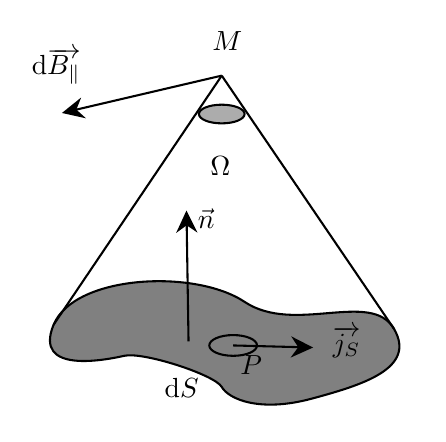
\begin{tikzpicture}[x=0.75pt,y=0.75pt,yscale=-1,xscale=1]
%uncomment if require: \path (0,485); %set diagram left start at 0, and has height of 485

%Shape: Polygon Curved [id:ds3922129264966643] 
\draw  [fill={rgb, 255:red, 128; green, 128; blue, 128 }  ,fill opacity=1 ] (284,241) .. controls (294,217) and (352,214) .. (376,230) .. controls (400,246) and (437,224) .. (448,243) .. controls (459,262) and (433,270) .. (408.19,276.68) .. controls (383.37,283.36) and (368.37,276.9) .. (365,271) .. controls (361.63,265.1) and (327.15,253.96) .. (318.08,255.98) .. controls (309,258) and (274,265) .. (284,241) -- cycle ;
%Straight Lines [id:da5617325667802913] 
\draw    (365,121) -- (448,243) ;
%Straight Lines [id:da5785428663305934] 
\draw    (365,121) -- (284,241) ;
%Shape: Ellipse [id:dp18923666125746497] 
\draw  [fill={rgb, 255:red, 155; green, 155; blue, 155 }  ,fill opacity=0.83 ] (354,139.5) .. controls (354,137.01) and (358.92,135) .. (365,135) .. controls (371.08,135) and (376,137.01) .. (376,139.5) .. controls (376,141.99) and (371.08,144) .. (365,144) .. controls (358.92,144) and (354,141.99) .. (354,139.5) -- cycle ;
%Straight Lines [id:da40958843225991837] 
\draw    (365,121) -- (290.92,138.32) ;
\draw [shift={(288,139)}, rotate = 346.84000000000003] [fill={rgb, 255:red, 0; green, 0; blue, 0 }  ][line width=0.08]  [draw opacity=0] (10.72,-5.15) -- (0,0) -- (10.72,5.15) -- (7.12,0) -- cycle    ;
%Straight Lines [id:da29389847237299893] 
\draw    (349,249) -- (348.05,189) ;
\draw [shift={(348,186)}, rotate = 449.09] [fill={rgb, 255:red, 0; green, 0; blue, 0 }  ][line width=0.08]  [draw opacity=0] (10.72,-5.15) -- (0,0) -- (10.72,5.15) -- (7.12,0) -- cycle    ;
%Shape: Ellipse [id:dp39374247527024986] 
\draw   (359,251) .. controls (359,248.24) and (364.15,246) .. (370.5,246) .. controls (376.85,246) and (382,248.24) .. (382,251) .. controls (382,253.76) and (376.85,256) .. (370.5,256) .. controls (364.15,256) and (359,253.76) .. (359,251) -- cycle ;
%Straight Lines [id:da8547868678069266] 
\draw    (370.5,251) -- (406,251.92) ;
\draw [shift={(409,252)}, rotate = 181.49] [fill={rgb, 255:red, 0; green, 0; blue, 0 }  ][line width=0.08]  [draw opacity=0] (10.72,-5.15) -- (0,0) -- (10.72,5.15) -- (7.12,0) -- cycle    ;

% Text Node
\draw (272,106.4) node [anchor=north west][inner sep=0.75pt]    {$\mathrm{d}\overrightarrow{B_{\parallel }}$};
% Text Node
\draw (359,98.4) node [anchor=north west][inner sep=0.75pt]    {$M$};
% Text Node
\draw (358,158.4) node [anchor=north west][inner sep=0.75pt]    {$\Omega $};
% Text Node
\draw (352,183.4) node [anchor=north west][inner sep=0.75pt]    {$\vec{n}$};
% Text Node
\draw (336,265.4) node [anchor=north west][inner sep=0.75pt]    {$\mathrm{d} S$};
% Text Node
\draw (372.5,254.4) node [anchor=north west][inner sep=0.75pt]    {$P$};
% Text Node
\draw (417,240.4) node [anchor=north west][inner sep=0.75pt]    {$\overrightarrow{j_{S}}$};


\end{tikzpicture}

\end{center}
Lại có $\ot{i}\mathrm{d}\ot{l}=I$, trong đó $\mathrm{d}\ot{I}$ là vi phân chiều rộng mà mật độ dòng đi qua.\\
Viết lại thì ta sẽ được:
$$\mathrm{d}\ot{B}=\dfrac{\mu_0}{4\pi}\cdot\dfrac{\ot{i}\cdot \mathrm{d}S\times\overline{PM}}{PM^3}.$$
Ta có: $\mathrm{d}\ot{B}=\mathrm{d}\ot{B_\parallel}+\mathrm{d}\ot{B_\bot}\Rightarrow{\mathrm{d}\ot{B_\parallel}}=\dd \ot{B}-\mathrm{d}\ot{B_\bot}$
\begin{align*}
   \mathrm{d}\ot{B_\bot}&=\left(\mathrm{d}\ot{B}\cdot\ot{n}\right)\cdot\ot{n},\\
    \mathrm{d}\ot{B}&=\left(\ot{n}\cdot\ot{n}\right)\cdot\ot{B}.
\end{align*}

Ta đã biết: $\ot{a}\times\left(\ot{b}\times\ot{c}\right)=\left(\ot{a}\cdot\ot{c}\right)\ot{b}-\left(\ot{a}\cdot\ot{b}\right)\cdot\ot{c}$.\\
Vậy $d\ot{B_\parallel}=\left(\ot{n}\cdot\ot{n}\right)\cdot \mathrm{d}\ot{B}-\left(d\mathrm{d}\ot{B}\cdot\ot{n}\right)\cdot\ot{n}=\ot{n}\times\left(\mathrm{d}\ot{B}\times\ot{n}\right)$.\\
Có
\begin{align*}
    \mathrm{d}\ot B \times \ot n &= \dfrac{{{\mu _0}}}{{4\pi }} \cdot \dfrac{{\ot \imath  \cdot \mathrm{d}S \times \ot {PM} }}{{P{M^3}}} \times \ot n \\&=  - \dfrac{{{\mu _0}}}{{4\pi }} \cdot \dfrac{{\ot \imath }}{{P{M^3}}} \cdot (\ot n \cdot \ot {PM} ) \cdot \mathrm{d}S \\&=  - \dfrac{{{\mu _0}}}{{4\pi }} \cdot \ot \imath  \cdot \mathrm{d}\Omega
\end{align*}
Dễ dàng suy ra được:
$$\mathrm{d}\ot{B_\parallel}=\dfrac{\mu_0}{4\pi}\cdot \ot{i}\cdot \mathrm{d}Q\times\ot{n}=\dfrac{\mu_0}{4\pi}\left(\ot{i}\times\ot{n}\right)\cdot \dd Q$$
Cách 2: Dùng sự phụ thuộc giữa điện và từ trường:\\
Ta biết rằng điện tích di chuyển với vận tốc $v$ thì sinh ra điện trường theo công thức:
$$\mathrm{d}\ot{B}=\mu_0\varepsilon_0\ot{v}\times\dfrac{\sigma \mathrm{d}S}{4\pi\varepsilon_0}\cdot\dfrac{\ot{r}}{r^3}.$$
Ta gọi vector đơn vị vuông góc vơi vector pháp tuyến và vuông góc với vector mật độ dòng $\ot{i}$ là $\ot{e_\parallel}$:
\begin{align*}
    \mathrm{d}\ot B &= \dfrac{{{\mu_0}}}{{4\pi }}\ot v \times \sigma \mathrm{d}S \cdot \dfrac{{\ot r}}{{{r^3}}}\\
\mathrm{d}\ot B \cdot \ot {{e_\parallel}}  &= \ot {{e_\parallel}}  \cdot \left( {\dfrac{{{\mu_0}}}{{4\pi }}\ot v \times \sigma \mathrm{d}S \cdot \dfrac{{\ot r}}{{{r^3}}}} \right)
\\&= \sigma \mathrm{d}S \cdot \dfrac{{\ot r}}{{{r^3}}} \cdot \left( {\dfrac{\mu_0}{4\pi }\ot v \times {{\ot e_\parallel}}} \right) \\&= \sigma \mathrm{d}S \cdot \dfrac{{\ot r}}{{{r^3}}} \cdot \dfrac{{{\mu _0}}}{{4\pi }} \cdot v \cdot \ot n
\end{align*}

Kết hợp định nghĩa $\ot{i}=\sigma\ot{v}$.\\
Vậy dễ dàng rút ra được:
\[{B} = \dfrac{{{\mu_0}}}{{4\pi }} \cdot i\Omega. \]
    \item 
    \begin{enumerate}[a)]
        \item Một ống solenoid thì ta lại có: $i\mathrm{d}L=\mathrm{d}I=N\cdot\dfrac{I \mathrm{d} L}{L}$.\\
        Vậy dễ dàng thấy được $i=\dfrac{NI}{L}=nI$.\\
        Đối với trong lòng của ống dây, từ trường gây ra bởi cuộn dây sẽ quét nên một góc khối trong toàn bộ không gian là $4\pi$.\\
        Từ trường trong trường hợp này là: $B=\dfrac{\mu_0}{4\pi}\cdot iQ=\mu_0nI$.
        \item Trường hợp ở sát một đầu dây thì góc khối bây giờ sẽ là $2\pi$.\\
        Tương tự như thế suy ra ngay được: $B=\dfrac{\mu_0nI}{2}$.
        \item Tại một điểm cách đoạn $x$ ở bên ngoài thì góc khối của nó bây giờ sẽ là như trên hình vẽ:
        \begin{center}
            

\tikzset{every picture/.style={line width=0.75pt}} %set default line width to 0.75pt        

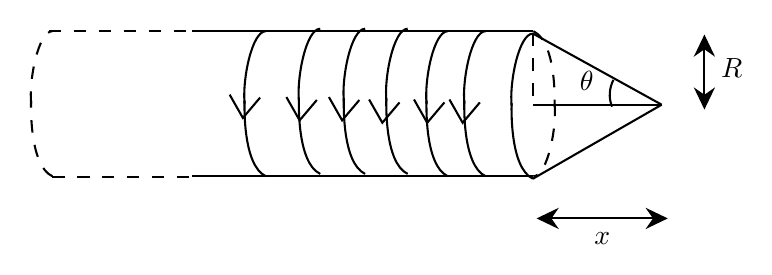
\begin{tikzpicture}[x=0.75pt,y=0.75pt,yscale=-1,xscale=1]
%uncomment if require: \path (0,404); %set diagram left start at 0, and has height of 404

%Curve Lines [id:da23246274003905754] 
\draw  [dash pattern={on 4.5pt off 4.5pt}]  (273.07,144.77) .. controls (284.48,150.19) and (283.34,179.92) .. (283.34,181.37) ;
%Curve Lines [id:da2569353747444356] 
\draw  [dash pattern={on 4.5pt off 4.5pt}]  (283.32,179.74) .. controls (284.48,190.99) and (279.93,214.6) .. (273.07,214.71) ;

%Curve Lines [id:da6183062170471916] 
\draw    (272.87,215.88) .. controls (261.46,210.46) and (262.6,180.73) .. (262.6,179.27) ;
%Curve Lines [id:da8296363002858504] 
\draw    (262.62,180.91) .. controls (261.46,169.66) and (266.01,146.05) .. (272.87,145.93) ;

%Straight Lines [id:da3261169614679926] 
\draw  [dash pattern={on 4.5pt off 4.5pt}]  (39.74,144.77) -- (108.81,144.77) ;
%Straight Lines [id:da9388131806363158] 
\draw    (108.81,214.71) -- (273.07,214.71) ;
%Straight Lines [id:da4981940820064006] 
\draw  [dash pattern={on 4.5pt off 4.5pt}]  (41.26,215.18) -- (110.33,215.18) ;
%Curve Lines [id:da058548510603747994] 
\draw  [dash pattern={on 4.5pt off 4.5pt}]  (41.36,214.71) .. controls (29.95,209.29) and (31.09,179.57) .. (31.09,178.11) ;
%Curve Lines [id:da28674009073319295] 
\draw  [dash pattern={on 4.5pt off 4.5pt}]  (31.12,179.74) .. controls (29.95,168.49) and (34.5,144.88) .. (41.36,144.77) ;
%Straight Lines [id:da13313345870106996] 
\draw    (108.81,144.77) -- (273.07,144.77) ;
%Curve Lines [id:da23687454756529425] 
\draw    (170.4,213.55) .. controls (158.99,208.13) and (160.12,178.4) .. (160.12,176.94) ;
%Curve Lines [id:da3437203023218134] 
\draw    (160.15,178.57) .. controls (158.99,167.32) and (163.54,143.72) .. (170.4,143.6) ;

%Curve Lines [id:da06407716040321243] 
\draw    (212.53,213.55) .. controls (201.11,208.13) and (202.25,178.4) .. (202.25,176.94) ;
%Curve Lines [id:da6035310173871988] 
\draw    (202.28,178.57) .. controls (201.11,167.32) and (205.67,143.72) .. (212.53,143.6) ;

%Curve Lines [id:da8494685484120488] 
\draw    (192.03,213.55) .. controls (180.62,208.13) and (181.76,178.4) .. (181.76,176.94) ;
%Curve Lines [id:da08931353505314421] 
\draw    (181.79,178.57) .. controls (180.62,167.32) and (185.17,143.72) .. (192.03,143.6) ;

%Curve Lines [id:da15702687900044277] 
\draw    (144.21,214.71) .. controls (132.8,209.29) and (133.94,179.57) .. (133.94,178.11) ;
%Curve Lines [id:da40233214034429454] 
\draw    (133.97,179.74) .. controls (132.8,168.49) and (137.35,144.88) .. (144.21,144.77) ;

%Curve Lines [id:da7723532534265405] 
\draw    (231.88,214.71) .. controls (220.47,209.29) and (221.61,179.57) .. (221.61,178.11) ;
%Curve Lines [id:da5932349698555781] 
\draw    (221.64,179.74) .. controls (220.47,168.49) and (225.02,144.88) .. (231.88,144.77) ;

%Curve Lines [id:da9159460175559413] 
\draw    (250.1,214.71) .. controls (238.69,209.29) and (239.82,179.57) .. (239.82,178.11) ;
%Curve Lines [id:da17927431896962043] 
\draw    (239.85,179.74) .. controls (238.69,168.49) and (243.24,144.88) .. (250.1,144.77) ;

\draw   (141.43,176.78) -- (133.14,186.58) -- (126.77,175.38) ;
\draw   (230.24,179.11) -- (221.95,188.91) -- (215.58,177.71) ;
\draw   (208.61,179.11) -- (200.32,188.91) -- (193.95,177.71) ;
\draw   (189.25,177.95) -- (180.96,187.75) -- (174.59,176.54) ;
\draw   (168.76,177.95) -- (160.47,187.75) -- (154.1,176.54) ;
\draw   (247.32,179.11) -- (239.03,188.91) -- (232.66,177.71) ;
%Straight Lines [id:da881459178130799] 
\draw    (272.87,180.21) -- (334.92,180.21) ;
%Straight Lines [id:da9432755276672973] 
\draw  [dash pattern={on 4.5pt off 4.5pt}]  (272.87,145.93) -- (272.87,180.21) ;
%Straight Lines [id:da45327501223814326] 
\draw    (272.87,145.93) -- (334.92,180.21) ;
%Straight Lines [id:da28880569926011423] 
\draw    (272.87,215.88) -- (334.92,180.21) ;
%Shape: Arc [id:dp3564037563549467] 
\draw  [draw opacity=0] (311.01,181.16) .. controls (310.95,181.01) and (310.89,180.85) .. (310.83,180.7) .. controls (309.28,176.61) and (309.71,172.18) .. (311.64,168.27) -- (328.08,173.87) -- cycle ; \draw   (311.01,181.16) .. controls (310.95,181.01) and (310.89,180.85) .. (310.83,180.7) .. controls (309.28,176.61) and (309.71,172.18) .. (311.64,168.27) ;
%Straight Lines [id:da8861979171919769] 
\draw    (277.66,235) -- (334.85,235) ;
\draw [shift={(337.85,235)}, rotate = 180] [fill={rgb, 255:red, 0; green, 0; blue, 0 }  ][line width=0.08]  [draw opacity=0] (10.72,-5.15) -- (0,0) -- (10.72,5.15) -- (7.12,0) -- cycle    ;
\draw [shift={(274.66,235)}, rotate = 0] [fill={rgb, 255:red, 0; green, 0; blue, 0 }  ][line width=0.08]  [draw opacity=0] (10.72,-5.15) -- (0,0) -- (10.72,5.15) -- (7.12,0) -- cycle    ;
%Straight Lines [id:da3805062587054828] 
\draw    (355.5,179.54) -- (355.5,149.4) ;
\draw [shift={(355.5,146.4)}, rotate = 450] [fill={rgb, 255:red, 0; green, 0; blue, 0 }  ][line width=0.08]  [draw opacity=0] (10.72,-5.15) -- (0,0) -- (10.72,5.15) -- (7.12,0) -- cycle    ;
\draw [shift={(355.5,182.54)}, rotate = 270] [fill={rgb, 255:red, 0; green, 0; blue, 0 }  ][line width=0.08]  [draw opacity=0] (10.72,-5.15) -- (0,0) -- (10.72,5.15) -- (7.12,0) -- cycle    ;


% Text Node
\draw (294,162.4) node [anchor=north west][inner sep=0.75pt]    {$\theta $};
% Text Node
\draw (362,156.4) node [anchor=north west][inner sep=0.75pt]    {$R$};
% Text Node
\draw (301,240.4) node [anchor=north west][inner sep=0.75pt]    {$x$};


\end{tikzpicture}

        \end{center}
        Lúc này góc khối $\Omega$ sẽ được tính bằng công thức:
        $$\Omega=2\pi(1-\mathrm{cos}\theta),$$
        với $$\mathrm{cos}\theta=\dfrac{x}{\sqrt{x^2+R^2}}.$$
        Vậy ta rút ra từ trường bên ngoài:
        \[\ot {{B_1}}  + \ot {{B_2}}  = \dfrac{j}{2}\left[ {\left( {\ot {{r_1}}  \times \ot {{e_z}} } \right) + \left( {\ot {{r_2}}  \times \ot {{e_z}} } \right)} \right].\]
        \item Trường hợp bên trong thì cũng làm tương tự với góc khối bây giờ là:
        \[B = \dfrac{{{\mu _0}}}{{4\pi }} \cdot i.2\pi \left( {1 + \dfrac{x}{{\sqrt {{x^2} + {R^2}} }}} \right) = \dfrac{{{\mu _0}nI}}{2}\left( {1 + \dfrac{x}{{\sqrt {{x^2} + {R^2}} }}} \right).\]
        \item Đối với từ trường của một ống dây dài hữu hạn, dựa vào hình vẽ, ta có thể xác định được góc khối trong trường hợp này là:
        \begin{center}
            

\tikzset{every picture/.style={line width=0.75pt}} %set default line width to 0.75pt        

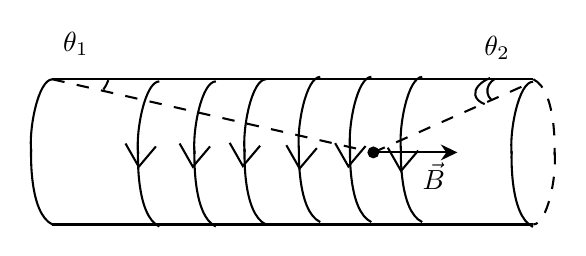
\begin{tikzpicture}[x=0.75pt,y=0.75pt,yscale=-1,xscale=1]
%uncomment if require: \path (0,424); %set diagram left start at 0, and has height of 424

%Curve Lines [id:da07323833825779236] 
\draw  [dash pattern={on 4.5pt off 4.5pt}]  (292.07,163.77) .. controls (303.48,169.19) and (302.34,198.92) .. (302.34,200.37) ;
%Curve Lines [id:da9496880182926646] 
\draw  [dash pattern={on 4.5pt off 4.5pt}]  (302.32,198.74) .. controls (303.48,209.99) and (298.93,233.6) .. (292.07,233.71) ;

%Curve Lines [id:da7476871733726151] 
\draw    (291.87,234.88) .. controls (280.46,229.46) and (281.6,199.73) .. (281.6,198.27) ;
%Curve Lines [id:da06025915165235585] 
\draw    (281.62,199.91) .. controls (280.46,188.66) and (285.01,165.05) .. (291.87,164.93) ;

%Straight Lines [id:da18234503170898786] 
\draw    (60.36,233.71) -- (292.07,233.71) ;
%Curve Lines [id:da0505559185628377] 
\draw    (60.36,233.71) .. controls (48.95,228.29) and (50.09,198.57) .. (50.09,197.11) ;
%Curve Lines [id:da5126057145976575] 
\draw    (50.12,198.74) .. controls (48.95,187.49) and (53.5,163.88) .. (60.36,163.77) ;
%Straight Lines [id:da08712239262055488] 
\draw    (60.36,163.77) -- (292.07,163.77) ;
%Curve Lines [id:da5064182955926819] 
\draw    (189.4,232.55) .. controls (177.99,227.13) and (179.12,197.4) .. (179.12,195.94) ;
%Curve Lines [id:da5726160887077749] 
\draw    (179.15,197.57) .. controls (177.99,186.32) and (182.54,162.72) .. (189.4,162.6) ;

%Curve Lines [id:da7540039118690092] 
\draw    (238.53,232.55) .. controls (227.11,227.13) and (228.25,197.4) .. (228.25,195.94) ;
%Curve Lines [id:da014194331336817356] 
\draw    (228.28,197.57) .. controls (227.11,186.32) and (231.67,162.72) .. (238.53,162.6) ;

%Curve Lines [id:da8258998787902145] 
\draw    (214.03,232.55) .. controls (202.62,227.13) and (203.76,197.4) .. (203.76,195.94) ;
%Curve Lines [id:da20967547716520074] 
\draw    (203.79,197.57) .. controls (202.62,186.32) and (207.17,162.72) .. (214.03,162.6) ;

%Curve Lines [id:da952782857362197] 
\draw    (163.21,233.71) .. controls (151.8,228.29) and (152.94,198.57) .. (152.94,197.11) ;
%Curve Lines [id:da34159559225433966] 
\draw    (152.97,198.74) .. controls (151.8,187.49) and (156.35,163.88) .. (163.21,163.77) ;

%Curve Lines [id:da13326939859262188] 
\draw    (111.88,234.71) .. controls (100.47,229.29) and (101.61,199.57) .. (101.61,198.11) ;
%Curve Lines [id:da4192039683738553] 
\draw    (101.64,199.74) .. controls (100.47,188.49) and (105.02,164.88) .. (111.88,164.77) ;

%Curve Lines [id:da31499361935964054] 
\draw    (139.1,234.71) .. controls (127.69,229.29) and (128.82,199.57) .. (128.82,198.11) ;
%Curve Lines [id:da015405963374842235] 
\draw    (128.85,199.74) .. controls (127.69,188.49) and (132.24,164.88) .. (139.1,164.77) ;

\draw   (160.43,195.78) -- (152.14,205.58) -- (145.77,194.38) ;
\draw   (110.24,196.11) -- (101.95,205.91) -- (95.58,194.71) ;
\draw   (236.61,198.11) -- (228.32,207.91) -- (221.95,196.71) ;
\draw   (211.25,195.95) -- (202.96,205.75) -- (196.59,194.54) ;
\draw   (187.76,196.95) -- (179.47,206.75) -- (173.1,195.54) ;
\draw   (136.32,196.11) -- (128.03,205.91) -- (121.66,194.71) ;
%Straight Lines [id:da13750396875137127] 
\draw    (215,199) -- (252.5,199) ;
\draw [shift={(255.5,199)}, rotate = 180] [fill={rgb, 255:red, 0; green, 0; blue, 0 }  ][line width=0.08]  [draw opacity=0] (8.04,-3.86) -- (0,0) -- (8.04,3.86) -- (5.34,0) -- cycle    ;
\draw [shift={(215,199)}, rotate = 0] [color={rgb, 255:red, 0; green, 0; blue, 0 }  ][fill={rgb, 255:red, 0; green, 0; blue, 0 }  ][line width=0.75]      (0, 0) circle [x radius= 2.34, y radius= 2.34]   ;
%Straight Lines [id:da13567381207390805] 
\draw  [dash pattern={on 4.5pt off 4.5pt}]  (215,199) -- (291.87,164.93) ;
%Straight Lines [id:da5589741252035714] 
\draw  [dash pattern={on 4.5pt off 4.5pt}]  (60.36,163.77) -- (215,199) ;
%Shape: Arc [id:dp9185533195236573] 
\draw  [draw opacity=0] (268.65,175.72) .. controls (266.14,174.79) and (264.44,173.26) .. (264.1,171.31) .. controls (263.58,168.28) and (266.53,165.08) .. (271.19,163.13) -- (277.67,168.98) -- cycle ; \draw   (268.65,175.72) .. controls (266.14,174.79) and (264.44,173.26) .. (264.1,171.31) .. controls (263.58,168.28) and (266.53,165.08) .. (271.19,163.13) ;
%Shape: Arc [id:dp8868817492672574] 
\draw  [draw opacity=0] (87.32,164.2) .. controls (86.73,165.82) and (85.93,167.33) .. (84.95,168.72) -- (69,157.5) -- cycle ; \draw   (87.32,164.2) .. controls (86.73,165.82) and (85.93,167.33) .. (84.95,168.72) ;
%Shape: Arc [id:dp29997511001655597] 
\draw  [draw opacity=0] (271.66,173.47) .. controls (270.79,172.61) and (270.19,171.53) .. (269.98,170.3) .. controls (269.52,167.62) and (271.04,164.99) .. (273.6,163.52) -- (277.67,168.98) -- cycle ; \draw   (271.66,173.47) .. controls (270.79,172.61) and (270.19,171.53) .. (269.98,170.3) .. controls (269.52,167.62) and (271.04,164.99) .. (273.6,163.52) ;

% Text Node
\draw (64,139.4) node [anchor=north west][inner sep=0.75pt]    {$\theta _{1}$};
% Text Node
\draw (267,141.4) node [anchor=north west][inner sep=0.75pt]    {$\theta _{2}$};
% Text Node
\draw (237.25,202.4) node [anchor=north west][inner sep=0.75pt]    {$\vec{B}$};
\end{tikzpicture}
        \end{center}
        Góc khối lúc này sẽ là:
        $$\Omega=4\pi-2\pi(1-\mathrm{cos}\theta_1)-2\pi(1-\mathrm{cos}\theta_2)=2\pi(\mathrm{cos}\theta_1+\mathrm{cos}\theta_2).$$
        Vậy từ trường gây ra lúc này sẽ là: $B=\dfrac{\mu_0}{2}nI(\mathrm{cos}\theta_1+\mathrm{cos}\theta_2)$.
    \end{enumerate}
\end{enumerate}
\end{loigiai}

\begin{vd}[Bẫy từ Ioffe $-$ Pritchard]
Bẫy từ Ioffe $-$ Pritchard được sử dụng để giam giữ các nguyên tử chuyển động, và có cấu tạo chính như hình vẽ. Bốn dây thẳng $1,2,3,4$ có dòng điện không đổi $I$, đặt vuông góc với mặt phẳng $x-y$, và giao của chúng với mặt phẳng $x-y$ là hình vuông cạnh $2 a$, tâm tại ${O}$, mặt phẳng chứa các dòng $1$ và $2$ song song với trục $x$, và chiều dòng điện trong mỗi dây được biểu diễn trên hình.
\begin{center}

\tikzset{every picture/.style={line width=0.75pt}} %set default line width to 0.75pt        

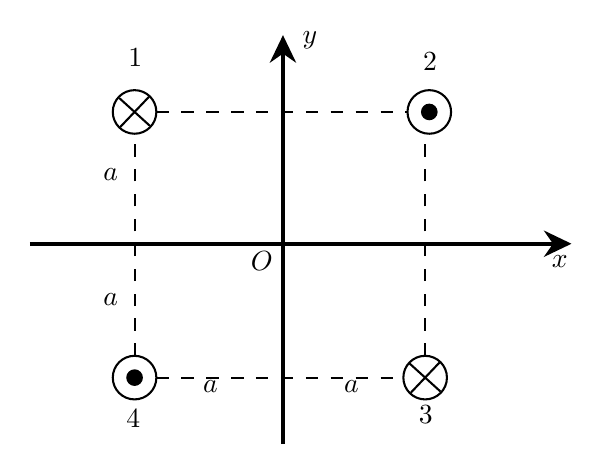
\begin{tikzpicture}[x=0.75pt,y=0.75pt,yscale=-1,xscale=1]
%uncomment if require: \path (0,300); %set diagram left start at 0, and has height of 300

%Straight Lines [id:da05626332961750413] 
\draw [line width=1.5]    (134,125) -- (391,125) ;
\draw [shift={(395,125)}, rotate = 180] [fill={rgb, 255:red, 0; green, 0; blue, 0 }  ][line width=0.08]  [draw opacity=0] (13.4,-6.43) -- (0,0) -- (13.4,6.44) -- (8.9,0) -- cycle    ;
%Straight Lines [id:da3913295804206024] 
\draw [line width=1.5]    (256,221.5) -- (256,28.5) ;
\draw [shift={(256,24.5)}, rotate = 450] [fill={rgb, 255:red, 0; green, 0; blue, 0 }  ][line width=0.08]  [draw opacity=0] (13.4,-6.43) -- (0,0) -- (13.4,6.44) -- (8.9,0) -- cycle    ;
%Shape: Circle [id:dp6160096759071784] 
\draw   (174,61.5) .. controls (174,55.7) and (178.7,51) .. (184.5,51) .. controls (190.3,51) and (195,55.7) .. (195,61.5) .. controls (195,67.3) and (190.3,72) .. (184.5,72) .. controls (178.7,72) and (174,67.3) .. (174,61.5) -- cycle ;
%Shape: Circle [id:dp4248456703533038] 
\draw   (174,189.5) .. controls (174,183.7) and (178.7,179) .. (184.5,179) .. controls (190.3,179) and (195,183.7) .. (195,189.5) .. controls (195,195.3) and (190.3,200) .. (184.5,200) .. controls (178.7,200) and (174,195.3) .. (174,189.5) -- cycle ;
%Shape: Circle [id:dp4019079511405811] 
\draw   (314,189.5) .. controls (314,183.7) and (318.7,179) .. (324.5,179) .. controls (330.3,179) and (335,183.7) .. (335,189.5) .. controls (335,195.3) and (330.3,200) .. (324.5,200) .. controls (318.7,200) and (314,195.3) .. (314,189.5) -- cycle ;
%Shape: Circle [id:dp013023629702595962] 
\draw   (316,61.5) .. controls (316,55.7) and (320.7,51) .. (326.5,51) .. controls (332.3,51) and (337,55.7) .. (337,61.5) .. controls (337,67.3) and (332.3,72) .. (326.5,72) .. controls (320.7,72) and (316,67.3) .. (316,61.5) -- cycle ;
%Straight Lines [id:da8802869723008931] 
\draw  [dash pattern={on 4.5pt off 4.5pt}]  (195,61.5) -- (316,61.5) ;
%Straight Lines [id:da4959208578996771] 
\draw  [dash pattern={on 4.5pt off 4.5pt}]  (195,189.5) -- (314,189.5) ;
%Straight Lines [id:da36959580046992413] 
\draw  [dash pattern={on 4.5pt off 4.5pt}]  (184.5,179) -- (184.5,72) ;
%Straight Lines [id:da7139861589940194] 
\draw  [dash pattern={on 4.5pt off 4.5pt}]  (324.5,179) -- (324.5,72.51) ;
%Shape: Circle [id:dp2606064295674281] 
\draw  [fill={rgb, 255:red, 0; green, 0; blue, 0 }  ,fill opacity=1 ] (181,189.5) .. controls (181,187.57) and (182.57,186) .. (184.5,186) .. controls (186.43,186) and (188,187.57) .. (188,189.5) .. controls (188,191.43) and (186.43,193) .. (184.5,193) .. controls (182.57,193) and (181,191.43) .. (181,189.5) -- cycle ;
%Shape: Circle [id:dp789809900665985] 
\draw  [fill={rgb, 255:red, 0; green, 0; blue, 0 }  ,fill opacity=1 ] (323,61.5) .. controls (323,59.57) and (324.57,58) .. (326.5,58) .. controls (328.43,58) and (330,59.57) .. (330,61.5) .. controls (330,63.43) and (328.43,65) .. (326.5,65) .. controls (324.57,65) and (323,63.43) .. (323,61.5) -- cycle ;
%Straight Lines [id:da6092298739639638] 
\draw    (177.08,54.77) -- (191.92,68.23) ;
%Straight Lines [id:da5634359696784248] 
\draw    (317.08,182.77) -- (331.92,196.23) ;
%Straight Lines [id:da810522003822946] 
\draw    (191.49,54.15) -- (177.51,68.85) ;
%Straight Lines [id:da32755087114217485] 
\draw    (331.49,182.15) -- (317.51,196.85) ;

% Text Node
\draw (264,21.4) node [anchor=north west][inner sep=0.75pt]    {$y$};
% Text Node
\draw (384,129.4) node [anchor=north west][inner sep=0.75pt]    {$x$};
% Text Node
\draw (180,29.4) node [anchor=north west][inner sep=0.75pt]    {$1$};
% Text Node
\draw (322,31.4) node [anchor=north west][inner sep=0.75pt]    {$2$};
% Text Node
\draw (320,201.4) node [anchor=north west][inner sep=0.75pt]    {$3$};
% Text Node
\draw (179,203.4) node [anchor=north west][inner sep=0.75pt]    {$4$};
% Text Node
\draw (168,87.4) node [anchor=north west][inner sep=0.75pt]    {$a$};
% Text Node
\draw (168,147.4) node [anchor=north west][inner sep=0.75pt]    {$a$};
% Text Node
\draw (216,189.4) node [anchor=north west][inner sep=0.75pt]    {$a$};
% Text Node
\draw (284,189.4) node [anchor=north west][inner sep=0.75pt]    {$a$};
% Text Node
\draw (239,127.4) node [anchor=north west][inner sep=0.75pt]    {$O$};


\end{tikzpicture}
\end{center}
Toàn bộ hệ được đặt trong từ trường đều $\ot{B}_{0}=B_{0} \ot{k} (\ot{k}$ là vector đơn vị theo trục $z$ ). Độ từ thẩm của chân không là $\mu_{0}.$ Xét tại điểm ${M}$ có tọa độ $(x, y)$ ở rất gần gốc toạ độ trong mặt phẳng $x-y$. Kí hiệu các vector $\ot{r}=\overrightarrow{{OM}}$, và $\ot{r}_{a}=\overrightarrow{{aM}}, \ot{R}_{a}=\overrightarrow{{aO}}$ là các
vector kẻ từ dòng điện $a$ $({a}=1,2,3,4)$ tới điểm ${M}$ và ${O}$.
\begin{enumerate}[1)]
\item Xác định biểu thức gần đúng của vector cảm ứng từ $\ot{B}_{1}$ gây ra bởi dòng điện $1$ tại ${M}$. Trong kết quả cuối cùng chỉ giữ lại số hạng bậc nhất với $\ot{r}$.\\
\textbf{Gợi ý:} sử dụng gần đúng $\dfrac{1}{|\ot{R}+\ot{r}|^{2}} \approx \dfrac{1}{R^{2}}-\dfrac{2 \ot{R} \cdot \ot{r}}{R^{4}} \text{ khi }|\ot{R}| \gg|\ot{r}|$.
\item  Xác định biểu thức gần đúng của vector cảm ứng từ $\ot{B}$ gây ra bởi cả bốn dòng điện tại ${M}$. Trong kết quả cuối cùng chỉ giữ lại số hạng bậc nhất với $x$ và $y$.
\item  Đặt một nguyên tử có khối lượng $m$ vào trong bẫy từ tại gần gốc tọa độ. Do hiệu ứng nghịch từ, năng lượng liên kết của nguyên tử trong bẫy từ tỷ lệ thuận với độ lớn của từ trường tổng hợp $\ot{B}_{\text {tot }}$ tại vị trí của nguyên tử, tức là năng lượng liên kết có dạng $V=\mu\left|\ot{B}_{\text {tot}}\right|, \mu$ là hằng số dương. Xác định tần số dao động điều hòa (nếu xảy ra) của nguyên tử quanh gốc ${O}$.
\end{enumerate}

\end{vd}
\begin{loigiai}
\begin{enumerate}[1)]
    \item  Hệ thức vector $\ot{r}_{1}=\ot{R}_{1}+\ot{r}$. Vector cảm ứng từ $\ot{B}_{1}$ gây ra bởi dòng điện $1$ tại ${M}$ có biểu thức:
\[
\begin{aligned}
\ot{B}_{1} &=\dfrac{\mu_{0} \ot{I}_{1} \times \ot{r}_{1}}{2 \pi r_{1}^{2}}=\dfrac{-\mu_{0} I \ot{k} \times\left(\ot{R}_{1}+\ot{r}\right)}{2 \pi\left(\ot{R}_{1}+\ot{r}\right)^{2}} \approx \dfrac{-\mu_{0} \mid \ot{k} \times\left(\ot{R}_{1}+\ot{r}\right)}{2 \pi}\left(\dfrac{1}{R_{1}^{2}}-\dfrac{2 \ot{R}_{1} \cdot \ot{r}}{R_{1}^{4}}\right) \\
&=\dfrac{\mu_{0} I \ot{k}}{2 \pi} \times\left[\dfrac{-\ot{R}_{1}}{R_{1}^{2}}+\dfrac{-\ot{r}}{R_{1}^{2}}+\dfrac{\ot{R}_{1}\left(2 \ot{R}_{1} \cdot \ot{r}\right)}{R_{1}^{4}}\right].
\end{aligned}
\]
\item  Lần lượt viết:
\[
\begin{array}{l}
\ot{B}_{2}=\dfrac{\mu_{0} I \ot{k}}{2 \pi} \times\left[\dfrac{\ot{R}_{2}}{R_{2}^{2}}+\dfrac{\ot{r}}{R_{2}^{2}}+\dfrac{-\ot{R}_{2}\left(2 \ot{R}_{2} \cdot \ot{r}\right)}{R_{2}^{4}}\right], \\
\ot{B}_{3}=\dfrac{\mu_{0} I \ot{k}}{2 \pi} \times\left[\dfrac{-\ot{R}_{3}}{R_{3}^{2}}+\dfrac{-\ot{r}}{R_{3}^{2}}+\dfrac{\ot{R}_{3}\left(2 \ot{R}_{3} \cdot \ot{r}\right)}{R_{3}^{4}}\right], \\
\ot{B}_{4}=\dfrac{\mu_{0} I \ot{k}}{2 \pi} \times\left[\dfrac{\ot{R}_{4}}{R_{4}^{2}}+\dfrac{\ot{r}}{R_{4}^{2}}+\dfrac{-\ot{R}_{4}\left(2 \ot{R}_{4} \cdot \ot{r}\right)}{R_{4}^{4}}\right].
\end{array}
\]
Nguyên lí chồng chập:
\[
\ot{B}=\ot{B}_{1}+\ot{B}_{2}+\ot{B}_{3}+\ot{B}_{4}.
\]
Nhận thấy, $\ot{R}_{1}=-\ot{R}_{3}, \ot{R}_{2}=-\ot{R}_{4}$, và $R_{a}^{2}=2 a^{2}$ nên biểu thức trên rút gọn chỉ còn một số hạng:
\begin{align*}
\ot{B}&=\dfrac{\mu_{0} I \ot{k}}{8 \pi a^{4}} \times\left[2 \ot{R}_{1}\left(2 \ot{R}_{1}, \ot{r}\right)-2 \ot{R}_{2}\left(2 \ot{R}_{2} \cdot \ot{r}\right)\right]\\
&=\dfrac{\mu_{0} I \ot{k}}{2 \pi a^{4}} \times\left[\ot{R}_{1}\left(\ot{R}_{1}, \ot{r}\right)-\ot{R}_{2}\left(\ot{R}_{2} \cdot \ot{r}\right)\right].
\end{align*}
Viết $\ot{R}_{1}=a \ot{i}-a \ot{j}, \ot{R}_{2}=-a \ot{i}-a \ot{j}$, và $\ot{r}=x \ot{i}+y \ot{j}$ rồi thực hiện nhân có hướng, rồi sau đó nhân vô hướng:
\begin{align*}
    \ot{B}&=\dfrac{\mu_{0} I}{2 \pi a^{3}}\left[(\ot{j}+\ot{i})\left(\ot{R}_{1} \cdot \ot{r}\right)+\left(\ot{j}-\ot{i}\right)\left(\ot{R}_{2}, \ot{r}\right)\right]\\&=\dfrac{\mu_{0} I}{2 \pi a^{3}}\left\{\ot{i}\left[\left(\ot{R}_{1}-\ot{R}_{2}\right) \cdot \ot{r}\right]+\ot{j}\left[\left(\ot{R}_{2}+\ot{R}_{1}\right) \cdot \ot{r}\right]\right\}\\
    &=\dfrac{\mu_{0} I}{2 \pi a^{3}}\left\{\ot{i}(2 a x)+\ot{j}[-2 a y]\right\}=\dfrac{\mu_{0} I}{\pi a^{2}}(x \ot{i}-y \ot{j}).
\end{align*}
\item  Từ trường tổng hợp tại gần gốc tọa độ:
\[
\ot{B}_{\mathrm{tot}}=\ot{B}+\ot{B}_{0} \approx \dfrac{\mu_{0} I}{\pi a^{2}}\left(x \ot{i}-y \ot{j}\right)+B_{0} \ot{k}.
\]
Độ lớn từ trường:
\[
\left|B_{\mathrm{tot}}\right|=\sqrt{B_{0}^{2}+\left(\dfrac{\mu_{0} I}{\pi a^{2}}\right)^{2}\left(x^{2}+y^{2}\right)} \approx B_{0}+\dfrac{1}{2 B_{0}}\left(\dfrac{\mu_{0} I}{\pi a^{2}}\right)^{2}\left(x^{2}+y^{2}\right).
\]
Thế năng tương tác của nguyên tử trong từ trường:
\[
V=\mu\left|B_{\mathrm{tot}}\right| \approx \mu B_{0}+\dfrac{1}{2} \dfrac{\mu}{B_{0}}\left(\dfrac{\mu_{0} I}{\pi a^{2}}\right)^{2}\left(x^{2}+y^{2}\right).
\]
Đây là thế điều hòa với hệ số hồi phục: \[k=\dfrac{\mu}{B_{0}}\left(\dfrac{\mu_{0} I}{\pi a^{2}}\right)^{2}.\]
Tần số dao động điều hòa: \[\omega=\sqrt{\dfrac{k}{m}}=\dfrac{\mu_{0} I}{\pi a^{2}} \sqrt{\dfrac{\mu}{m B_{0}}}.\]
\end{enumerate}
\end{loigiai}


\newpage
    \begin{vd}[Khoảng cách giữa tôi và crush]
    Hai electron ở trong một điện trường đều $\ot{E}=E_0\ot{k}$ với $E_0=10^{-11}\dv{V/m}$. Một electron thì nằm ở gốc tọa độ, electron còn lại cách electron này $10\dv{m}$ về phía trên. Lúc đầu electron tại gốc tọa độ có vận tốc $u=10\dv{m/s}$ tạo với đường nối hai electron một góc $30^\circ$ như hình vẽ. Electron còn lại đứng yên tại thời điểm $t=0$. Tìm khoảng cách nhỏ nhất giữa hai electron trong quá trình chuyển động. Bỏ qua các hiện tượng tương đối tính. 
       \begin{center}

\begin{tikzpicture}[x=0.75pt,y=0.75pt,yscale=-1,xscale=1]
%uncomment if require: \path (0,205); %set diagram left start at 0, and has height of 205

%Shape: Circle [id:dp18323336474978213] 
\draw  [fill={rgb, 255:red, 0; green, 0; blue, 0 }  ,fill opacity=0 ] (336.1,35.68) .. controls (336.1,27.94) and (342.37,21.67) .. (350.11,21.67) .. controls (357.85,21.67) and (364.13,27.94) .. (364.13,35.68) .. controls (364.13,43.42) and (357.85,49.7) .. (350.11,49.7) .. controls (342.37,49.7) and (336.1,43.42) .. (336.1,35.68) -- cycle ;
%Shape: Circle [id:dp6394014267467758] 
\draw  [fill={rgb, 255:red, 0; green, 0; blue, 0 }  ,fill opacity=0 ] (336.1,160.68) .. controls (336.1,152.94) and (342.37,146.67) .. (350.11,146.67) .. controls (357.85,146.67) and (364.13,152.94) .. (364.13,160.68) .. controls (364.13,168.42) and (357.85,174.7) .. (350.11,174.7) .. controls (342.37,174.7) and (336.1,168.42) .. (336.1,160.68) -- cycle ;
%Straight Lines [id:da5720029831780469] 
\draw  [dash pattern={on 4.5pt off 4.5pt}]  (350.11,118.33) -- (350.11,160.68) ;
%Straight Lines [id:da10490696877725925] 
\draw    (384.34,103.24) -- (350.11,160.68) ;
\draw [shift={(385.36,101.53)}, rotate = 120.79] [color={rgb, 255:red, 0; green, 0; blue, 0 }  ][line width=0.75]    (10.93,-4.9) .. controls (6.95,-2.3) and (3.31,-0.67) .. (0,0) .. controls (3.31,0.67) and (6.95,2.3) .. (10.93,4.9)   ;
%Shape: Arc [id:dp8502310517364076] 
\draw  [draw opacity=0] (350.57,131.98) .. controls (355.68,132.06) and (360.46,133.48) .. (364.58,135.89) -- (350.11,160.68) -- cycle ; \draw   (350.57,131.98) .. controls (355.68,132.06) and (360.46,133.48) .. (364.58,135.89) ;
%Straight Lines [id:da6543877056659144] 
\draw    (271,159.9) -- (271,33.9) ;
\draw [shift={(271,31.9)}, rotate = 450] [color={rgb, 255:red, 0; green, 0; blue, 0 }  ][line width=0.75]    (10.93,-3.29) .. controls (6.95,-1.4) and (3.31,-0.3) .. (0,0) .. controls (3.31,0.3) and (6.95,1.4) .. (10.93,3.29)   ;
%Straight Lines [id:da32810999109005046] 
\draw    (190,159.9) -- (190,33.9) ;
\draw [shift={(190,31.9)}, rotate = 450] [color={rgb, 255:red, 0; green, 0; blue, 0 }  ][line width=0.75]    (10.93,-3.29) .. controls (6.95,-1.4) and (3.31,-0.3) .. (0,0) .. controls (3.31,0.3) and (6.95,1.4) .. (10.93,3.29)   ;
%Straight Lines [id:da9203020428315634] 
\draw    (512.28,159.9) -- (512.28,33.9) ;
\draw [shift={(512.28,31.9)}, rotate = 450] [color={rgb, 255:red, 0; green, 0; blue, 0 }  ][line width=0.75]    (10.93,-3.29) .. controls (6.95,-1.4) and (3.31,-0.3) .. (0,0) .. controls (3.31,0.3) and (6.95,1.4) .. (10.93,3.29)   ;
%Straight Lines [id:da028979424325561665] 
\draw    (431.28,159.9) -- (431.28,33.9) ;
\draw [shift={(431.28,31.9)}, rotate = 450] [color={rgb, 255:red, 0; green, 0; blue, 0 }  ][line width=0.75]    (10.93,-3.29) .. controls (6.95,-1.4) and (3.31,-0.3) .. (0,0) .. controls (3.31,0.3) and (6.95,1.4) .. (10.93,3.29)   ;

% Text Node
\draw (355.16,110.95) node [anchor=north west][inner sep=0.75pt]   [align=left] {$\displaystyle \theta $};
% Text Node
\draw (200,25) node [anchor=north west][inner sep=0.75pt]   [align=left] {$\displaystyle \overrightarrow{E}$};
\end{tikzpicture}
    \end{center}
    \end{vd}
    
    \begin{loigiai}\\
    \begin{minipage}{0.5\textwidth}
         Xét tại một thời điểm bất kì.\\
    Từ định luật II Newton, ta có:
    \begin{equation*}
        \begin{aligned}
             \ot{a_1}&=\dfrac{\ot{F}}{m_e}-\dfrac{\ot{E}e}{m_e},\\
             \ot{a_2}&=\dfrac{\ot{F'}}{m_e}-\dfrac{\ot{E}e}{m_e}.
        \end{aligned}
    \end{equation*}  
    \end{minipage}
    \begin{minipage}{0.5\textwidth}
         
\tikzset{every picture/.style={line width=0.75pt}} %set default line width to 0.75pt        

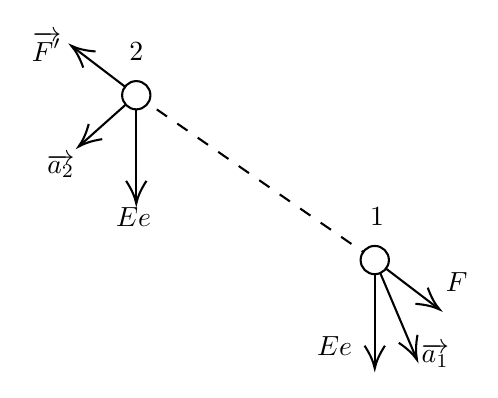
\begin{tikzpicture}[x=0.75pt,y=0.75pt,yscale=-1,xscale=1]
%uncomment if require: \path (0,205); %set diagram left start at 0, and has height of 205

%Straight Lines [id:da5983446918253625] 
\draw    (296.91,49.08) -- (267.25,26.47) ;
\draw [shift={(265.65,25.26)}, rotate = 397.31] [color={rgb, 255:red, 0; green, 0; blue, 0 }  ][line width=0.75]    (10.93,-4.9) .. controls (6.95,-2.3) and (3.31,-0.67) .. (0,0) .. controls (3.31,0.67) and (6.95,2.3) .. (10.93,4.9)   ;
%Straight Lines [id:da3352308238660524] 
\draw    (441.48,151.1) -- (411.81,128.49) ;
\draw [shift={(443.07,152.31)}, rotate = 217.31] [color={rgb, 255:red, 0; green, 0; blue, 0 }  ][line width=0.75]    (10.93,-4.9) .. controls (6.95,-2.3) and (3.31,-0.67) .. (0,0) .. controls (3.31,0.67) and (6.95,2.3) .. (10.93,4.9)   ;
%Straight Lines [id:da23872244936919795] 
\draw    (296.91,99.28) -- (296.91,49.08) ;
\draw [shift={(296.91,101.28)}, rotate = 270] [color={rgb, 255:red, 0; green, 0; blue, 0 }  ][line width=0.75]    (10.93,-4.9) .. controls (6.95,-2.3) and (3.31,-0.67) .. (0,0) .. controls (3.31,0.67) and (6.95,2.3) .. (10.93,4.9)   ;
%Straight Lines [id:da24870112119482535] 
\draw    (411.81,178.7) -- (411.81,128.49) ;
\draw [shift={(411.81,180.7)}, rotate = 270] [color={rgb, 255:red, 0; green, 0; blue, 0 }  ][line width=0.75]    (10.93,-4.9) .. controls (6.95,-2.3) and (3.31,-0.67) .. (0,0) .. controls (3.31,0.67) and (6.95,2.3) .. (10.93,4.9)   ;
%Straight Lines [id:da28480607533285895] 
\draw    (296.91,49.08) -- (270.59,72.53) ;
\draw [shift={(269.1,73.86)}, rotate = 318.3] [color={rgb, 255:red, 0; green, 0; blue, 0 }  ][line width=0.75]    (10.93,-4.9) .. controls (6.95,-2.3) and (3.31,-0.67) .. (0,0) .. controls (3.31,0.67) and (6.95,2.3) .. (10.93,4.9)   ;
%Straight Lines [id:da7214740206392896] 
\draw    (411.81,128.49) -- (431.37,174.66) ;
\draw [shift={(432.15,176.51)}, rotate = 247.04000000000002] [color={rgb, 255:red, 0; green, 0; blue, 0 }  ][line width=0.75]    (10.93,-4.9) .. controls (6.95,-2.3) and (3.31,-0.67) .. (0,0) .. controls (3.31,0.67) and (6.95,2.3) .. (10.93,4.9)   ;
%Straight Lines [id:da8071546537814793] 
\draw [fill={rgb, 255:red, 255; green, 255; blue, 255 }  ,fill opacity=1 ] [dash pattern={on 4.5pt off 4.5pt}]  (296.91,49.08) -- (411.81,128.49) ;
%Shape: Ellipse [id:dp9393753700341947] 
\draw  [fill={rgb, 255:red, 255; green, 255; blue, 255 }  ,fill opacity=1 ] (290.1,49.08) .. controls (290.1,45.32) and (293.15,42.27) .. (296.91,42.27) .. controls (300.67,42.27) and (303.72,45.32) .. (303.72,49.08) .. controls (303.72,52.84) and (300.67,55.89) .. (296.91,55.89) .. controls (293.15,55.89) and (290.1,52.84) .. (290.1,49.08) -- cycle ;
%Shape: Circle [id:dp6811911812920686] 
\draw  [fill={rgb, 255:red, 255; green, 255; blue, 255 }  ,fill opacity=1 ] (405,128.49) .. controls (405,124.73) and (408.05,121.68) .. (411.81,121.68) .. controls (415.57,121.68) and (418.62,124.73) .. (418.62,128.49) .. controls (418.62,132.25) and (415.57,135.3) .. (411.81,135.3) .. controls (408.05,135.3) and (405,132.25) .. (405,128.49) -- cycle ;

% Text Node
\draw (252.38,76.06) node [anchor=north west][inner sep=0.75pt]    {$\overrightarrow{a_{2}}$};
% Text Node
\draw (432.76,167.23) node [anchor=north west][inner sep=0.75pt]    {$\overrightarrow{a_{1}}$};
% Text Node
\draw (245.09,17.03) node [anchor=north west][inner sep=0.75pt]    {$\overrightarrow{F'}$};
% Text Node
\draw (444.55,133) node [anchor=north west][inner sep=0.75pt]    {$\ot{F}$};
% Text Node
\draw (285.67,101.83) node [anchor=north west][inner sep=0.75pt]    {$\ot{E} e$};
% Text Node
\draw (382.57,163.93) node [anchor=north west][inner sep=0.75pt]    {$\ot{E} e$};
% Text Node
\draw (408.04,101.8) node [anchor=north west][inner sep=0.75pt]    {$1$};
% Text Node
\draw (292.04,22.4) node [anchor=north west][inner sep=0.75pt]    {$2$};

\end{tikzpicture}
\vspace{5mm}
    \end{minipage}
    Xét trong hệ quy chiếu gắn với electron 2.
    Gia tốc của electron 1 so với electron 2
    $$\ot{a_{12}}=\ot{a_1}-\ot{a_2}=\dfrac{2\ot{F}}{m_e}.$$
    Ta thấy trong hệ quy chiếu gắn với electron 2 thì ta có thể coi như electron 2 là cố định còn electron 1 có khối lượng hiệu dụng $m=\dfrac{m_e}{2}$.
    Bảo toàn moment động lượng:
    \[ur_0\sin\theta=u_{\min}r_{\min}. \tag{1}\label{c131}\]
    Bảo toàn năng lượng:
    \[ \dfrac{ke^2}{r_0}+\dfrac{mu^2}{2}=\dfrac{ke^2}{r_{\min}}+\dfrac{m{u_{\min}^2}}{2}. \tag{2}\label{c132}\]
    Từ (\ref{c131}) và (\ref{c132}) ta có
    $$\tron{\dfrac{ke^2}{r_0}+\dfrac{mu^2}{2}}r_{min}^2-ke^2r_{\min}^2-\dfrac{mu^2{r_0}^2\sin^2\theta}{2}=0.$$
    Giải phương trình trên ta được $r_{\min}=6,84\dv{m}$.
    \end{loigiai}
    
\begin{vd}[Hợp nhất solenoid]
Hai cuộn solenoid hình trụ được đặt rất gần nhau sau cho chúng có chung một trục đối xứng (như hình vẽ). Hai cuộn dây giống hệt nhau, với tiết diện cắt $A$, và có mật độ $n$ vòng trên một đơn vị chiều dài. Cho dòng điện $I_1$ chạy qua một cuộn dây và dòng $I_2$ chạy qua cuộn dây còn lại. Tìm độ lớn lực từ giữa chúng.
\begin{center}
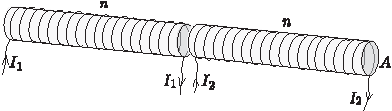
\includegraphics[scale=1.5]{Anh/Nam1.pdf}
\end{center}
\end{vd}
\begin{loigiai}
    \begin{itemize}
        \item \textbf{Cách 1:}
        \\  Áp dụng nguyên lí chồng chất, ta có thể dễ dàng suy ra từ thông qua một đầu cuộn dây bằng một nửa so với từ thông trong lòng ống dây. Do đó, theo cách sắp xếp cuộn dây như đề bài, từ thông của cuộn dây thứ nhất sẽ đi vào cuộn dây thứ hai và giá trị từ thông liên kết đó là
        \[\Phi=\dfrac{1}{2}\mu_0I_1nA.\]
        Một cách trực quan, toàn bộ từ thông từ cuộn $1$ đi vào cuộn $2$ sẽ đi ra ở mặt bên của cuộn vì nếu cuộn dây thứ hai là dài thì lượng từ thông đi ra ngoài ở đầu bên kia cuộn dây có thể được bỏ qua.
        \\Bây giờ chúng ta tính toán lực do từ trường của cuộn dây thứ nhất tác dụng lên dây dẫn mang dòng điện ở cuộn dây thứ hai. Thành phần từ trường dọc theo trục của cuộn dây không gây ra lực hiệu dụng lên cuộn dây $2$ vì lực từ do nó sinh ra xuyên tâm và đối xứng nên sẽ triệt tiêu lẫn nhau, do đó ở đây chúng ta chỉ tập trung vào thành phần từ trường theo phương xuyên tâm.
        \\Đặt thành phần xuyên tâm của vector cường độ từ trường tại vòng dây thứ $i$ tính từ đầu cuộn dây thứ hai là $B_i$. Do đó độ lớn của lực từ do cuộn dây thứ nhất tác dụng lên các vòng của cuộn dây thứ hai, mỗi vòng có bán kính $R$ và độ dài $2\pi R=2 \pi \sqrt{A/\pi}=2\sqrt{\pi A}$ là $F_i=2\sqrt{\pi A}I_2B_i$, do đó lực tác dụng lên toàn bộ cuộn dây thứ hai là
        \[F = \sum\limits_i {{F_i}}  = 2\sqrt {\pi A} {I_2}\sum\limits_i {{B_i}}.\]
        Tuy nhiên, chúng ta đã biết lượng từ thông từ cuộn dây $1$ thoát ra khỏi các mặt bên của cuộn dây $2$. Vì cuộn dây được cuốn $n$ vòng trên một đơn vị dài nên chúng ta có thể coi độ dày của một vòng là $1/n$, và diện tích bề mặt của mỗi vòng là $2\pi R/n = 2\sqrt {\pi A} /n$. Cuối cùng ta có biểu thức từ thông
        \[\frac{1}{2}{\mu _0}{I_1}nA = \Phi  = \sum\limits_i {\left( {\frac{{2\sqrt {\pi A} }}{n}{B_i}} \right).} \]
        So sánh giữa biểu thức lực và biểu thức từ thông ta thu được biểu thức độ lớn của lực từ
        \[F = \frac{1}{2}{\mu _0}{I_1}{I_2}{n^2}A.\]
        Nếu cả hai cuộn dây được cuốn theo cùng chiều, và chiều dòng điện như nhau thì lực giữa hai cuộn dây là lực hút. Nếu một trong hai thông số trên là ngược lại, thì lực là lực đẩy.
        \item \textbf{Cách 2:}
        \\Lực tương tác giữa hai cuộn dây sẽ tỉ lệ thuận với $I_1$ và $I_2$, vì từ trường sẽ tỉ lệ thuận với dòng điện trong một cuộn dây và từ trường đó gây lực từ lên dòng điện trong cuộn dây còn lại mà lực từ lại tỉ lệ thuận với tích $I.B$. Do đó ta có thể viết lực tương tác giữa hai cuộn dây theo dạng $F=K.I_1.I_2$, trong đó $K$ chỉ phụ thuộc vào các thông số cuộn dây và độc lập so với dòng điện chạy trong mỗi cuộn dây. Chúng ta sẽ rút ra K bằng cách tính toán lực tương tác trong trường hợp đặc biệt $I_1=I_2=I$, và hằng số $K$ đó là đúng cho mọi giá trị dòng điện.
        \\Giá trị lực từ chỉ phụ thuộc vào độ lớn của dòng điện chứ không phụ thuộc vào cách mà dòng điện đó được tạo ra. Nếu ta làm lạnh một cách phù hợp, cuộn dây mang dòng điện sẽ thành cuộn dây siêu dẫn (có điện trở = 0), và hai đầu cuộn dây sẽ hợp nhất thành một cuộn dây duy nhất có độ dài gấp đôi, và dòng điện sẽ là $I$ ở mọi nơi. Vì cuộn dây là siêu dẫn nên dòng điện $I$ sẽ không thay đổi dù không có bất kì nguồn cấp năng lượng nào. Bên trong cuộn dây, độ lớn của từ trường là $B=\mu_0nI$ và năng lượng từ trường được dự trữ là 
        \[{{{W}}_{\text{từ}}} = \frac{1}{{2{\mu _0}}}{B^2}V,\]
        ở đây $V=\ell A$ là thể tích của cuộn dây đôi có tiết diện mặt cắt $a$ và độ dài $\ell$. Chúng ta sẽ bàn kĩ hơn về vấn đề này ở phần mở rộng $1$.
        \\Điều gì sẽ xảy ra nếu chúng ta dịch hai cuộn solenoid ra cách xa nhau một đoạn $\Delta x(x\ll \ell)$. Từ trường trong ống dây tất yếu không thể thay đổi vì nếu có nó sẽ gây ra suất điện động cảm ứng và do cuộn dây không có điện trở nên dòng điện trong cuộn dây sẽ tiến đến vô cùng, đây là một hiện tượng phi vật lí. Nhưng năng lượng từ trường tích trữ trong cuộn dây thì có thay đổi, vì từ trường trong đoạn nhỏ đó bằng đúng từ trường trong lòng ống dây nhưng thể tích vùng từ trường lúc này tăng lên một khoảng nhỏ $\Delta V=A \Delta x.$
        \\Do đó phần năng lượng tăng lên tương ứng là 
        \[\Delta {W_{magn}} = \frac{1}{{2{\mu _0}}}{B^2}\Delta V = \frac{1}{2}{\mu _0}{I^2}{n^2}A\Delta x.\]
        Phần tăng năng lượng này chính bằng công của lực dùng để kéo ống dây ra, $W=F.\Delta x$, từ đây ta có thể suy ra 
        \[F = K{I_1}{I_2} = \frac{1}{2}{\mu _0}{I_1}{I_2}{n^2}A.\]
        \item \textbf{Mở rộng}
        \begin{itemize}
            \item  Hiệu ứng rìa không làm thay đổi kết quả vì nếu ta dịch cuộn dây ra xa nhau một khoảng nhỏ thì rìa cuộn dây cũng sẽ dịch đi một đoạn tương ứng. Do đó hiệu ứng rìa không làm ảnh hưởng đến phần thay đổi năng lượng.
            \item Một kết quả tương tự cũng có thể được tìm ra mà không cần đến hiện tượng siêu dẫn. Nối hai đầu cuộn dây lại ở điểm cuối của chúng để tạo thành một cuộn dây duy nhất thì lúc này sẽ có một dòng điện $I$ như nhau chạy trong cả hai cuộn dây. Nếu hai cuộn dây được kết nối theo cách này dịch ra xa nhau một khoảng nhỏ thì trên thực tế, từ trường và do đó từ thông ở khoảng đó sẽ bị giảm đi một chút vì việc ta dịch cuộn dây đi sẽ tạo thành một dòng điện cảm ứng rất nhỏ ngược chiều với dòng điện ban đầu, do đó làm giảm từ trường đi một lượng nhỏ.
            \\Chúng ta có thể chứng minh được năng lượng dự trữ của cuộn dây sẽ giảm đi một chút dù công thực hiện là dương. Hiện tượng kì lạ này có thể được giải thích bằng suất điện động cảm ứng gây ra bởi sự thay đổi từ thông. Sự giảm của suất điện động cảm ứng tương đương với việc năng lượng sẽ truyền vào cho nguồn điện và năng lượng này gấp đôi năng lượng giảm đi trên cuộn dây do đó công mà lực kéo sinh ra đã được truyền cho nguồn điện và giá trị của lực $F$ ta tính được lúc này vẫn như cách tiếp cận siêu dẫn.
        \end{itemize}

        
    \end{itemize}

\end{loigiai}

\begin{vd}[Định hướng sai]%Câu 6
Một vòng kim loại hình tròn có bán kính $r=0,1 \mathrm{m}$, quay quanh trục thẳng đứng là một đường kính của vòng với vận tốc góc không đổi. Như trên hình vẽ, một kim nam châm nhỏ đặt tại tâm vòng có thể quay tự do quanh trục thẳng đứng.
\begin{center}
\tikzset{every picture/.style={line width=0.75pt}} %set default line width to 0.75pt        

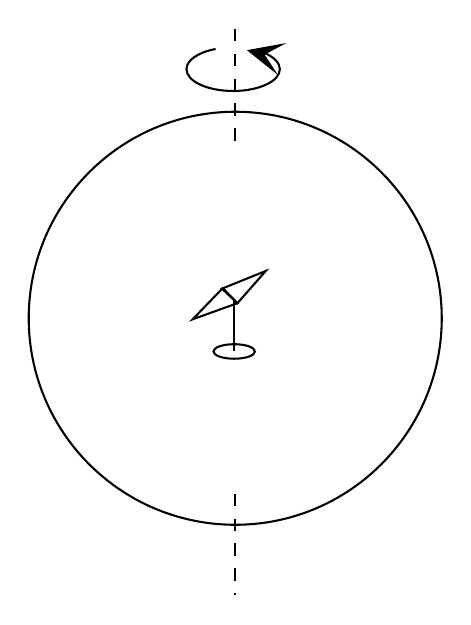
\begin{tikzpicture}[x=0.75pt,y=0.75pt,yscale=-1,xscale=1]
%uncomment if require: \path (0,420); %set diagram left start at 0, and has height of 420

%Shape: Circle [id:dp32204695616182843] 
\draw   (134,212.5) .. controls (134,157.55) and (178.55,113) .. (233.5,113) .. controls (288.45,113) and (333,157.55) .. (333,212.5) .. controls (333,267.45) and (288.45,312) .. (233.5,312) .. controls (178.55,312) and (134,267.45) .. (134,212.5) -- cycle ;
%Straight Lines [id:da17745998464492474] 
\draw  [dash pattern={on 4.5pt off 4.5pt}]  (233.5,73) -- (233.5,129) ;
%Straight Lines [id:da12402397940171284] 
\draw  [dash pattern={on 4.5pt off 4.5pt}]  (233.5,297) -- (233.5,346) ;
%Shape: Arc [id:dp723976575905914] 
\draw  [draw opacity=0] (248.07,84.92) .. controls (252.34,86.83) and (255,89.52) .. (255,92.5) .. controls (255,98.3) and (244.93,103) .. (232.5,103) .. controls (220.07,103) and (210,98.3) .. (210,92.5) .. controls (210,88.1) and (215.8,84.33) .. (224.04,82.77) -- (232.5,92.5) -- cycle ; \draw   (248.07,84.92) .. controls (252.34,86.83) and (255,89.52) .. (255,92.5) .. controls (255,98.3) and (244.93,103) .. (232.5,103) .. controls (220.07,103) and (210,98.3) .. (210,92.5) .. controls (210,88.1) and (215.8,84.33) .. (224.04,82.77) ;
\draw  [fill={rgb, 255:red, 0; green, 0; blue, 0 }  ,fill opacity=1 ] (252,93) -- (240.27,83.63) -- (255.05,80.96) -- (246.9,85.3) -- cycle ;
%Shape: Ellipse [id:dp25997108709859207] 
\draw   (223,228.5) .. controls (223,226.57) and (227.48,225) .. (233,225) .. controls (238.52,225) and (243,226.57) .. (243,228.5) .. controls (243,230.43) and (238.52,232) .. (233,232) .. controls (227.48,232) and (223,230.43) .. (223,228.5) -- cycle ;
%Straight Lines [id:da4944580997045749] 
\draw    (233,203.5) -- (233,228.5) ;
%Shape: Triangle [id:dp31251700899507884] 
\draw   (213,213) -- (227.49,197.98) -- (234.55,205.25) -- cycle ;
%Shape: Triangle [id:dp5236465704841922] 
\draw   (248.2,189.73) -- (234.55,205.25) -- (227.1,198.24) -- cycle ;





\end{tikzpicture}

\end{center}
Khi vòng đứng yên, kim nam châm chỉ theo hướng của thành phần nằm ngang của từ trường Trái Đất. Tuy nhiên, khi vòng quay với tốc độ mười vòng một giây, kim nam châm bị quay đi một góc $2^\circ$ so với ban đầu. Tính điện trở $R$ của vòng kim loại này.
\end{vd}
\begin{loigiai}
Phân tích từ trường Trái Đất thành các thành phần ngang và dọc. Thành phần dọc không gây ra dòng điện trong vòng, vì từ thông của nó gửi qua vòng luôn luôn bằng không. Đặt thành phần nằm ngang của từ trường là $B$ và vận tốc góc của vòng là  $\omega$. Từ thông gửi qua vòng là
$$\Phi=\pi{r^2}B\mathrm{cos}\omega t,$$
và suất điện động cảm ứng là $$ V=-\left(\dfrac{\dd\Phi}{\dd t}\right)=\pi{r^2}B\omega\mathrm{sin}\omega t.$$ Dòng điện có cường độ
$$ I=\dfrac{V}{R}=\dfrac{r^2\pi B\omega}{R}\mathrm{sin}\omega t,$$
chạy trong vòng gây ra một từ trường ở tâm vòng có độ lớn
$$B_I=\mu_0\dfrac{I}{2r}=\mu_0\dfrac{\pi rB\omega}{2R}\mathrm{sin}\omega t.$$
Từ trường $B_I$ có hướng vuông góc với mặt phẳng của vòng và quay cùng với nó. Phân tích vector $\ot{B_I}$ thành một thành phần song song $B$ và một thành phần vuông góc với nó. Thành phần song song tỉ lệ với $\mathrm{cos}\omega t\times\mathrm{sin}\omega t=\dfrac{1}{2}\mathrm{sin} 2\omega t$, trung bình bằng $0$ theo thời gian. Thành phần vuông góc có thể được viết là
$$B_{\bot}=\mu_0\dfrac{\pi rB\omega}{2R}{\mathrm{sin}^2}\omega t=\mu_0\dfrac{\pi rB\omega}{4R}\left(1-\mathrm{cos} 2\omega t\right).$$
Biểu thức này bao gồm một thành phần thay đổi (tương đối nhanh) theo thời gian và có trung bình là $0$, và một thành phần không đổi làm cho kim nam châm lệch đi  $\alpha = 2 ^\circ$ so với hướng ban đầu (bắc – nam). Vì kim nam châm hướng theo chiều của trường tổng hợp,
$$\tan\alpha=\dfrac{B_{\bot}}{B}=\mu_0\dfrac{\pi r\omega}{4R}.$$
Kim sẽ dao động nhỏ xung quanh vị trí trên, với biên độ được xác định bởi các đặc tính cơ học và từ tính của kim và bởi các lực giảm xóc. Thật thú vị khi để ý rằng góc lệch của kim nam châm không phụ thuộc vào độ lớn của từ trường Trái Đất. Điều quan trọng duy nhất là thành phần nằm ngang của nó là khác không. Điện trở của vòng có thể tính được từ công thức trên và có kết quả là $ 1,78\times{10^{-4}}\Omega.$
\end{loigiai}


\begin{vd}[Lồng hai solenoid]
     Một nhà khoa học làm thí nghiệm với hai ống dây solenoid đồng trục. Hai ống dây đều dài $l$, bán kính hai ống dây là $r$ và $2r$, ống nhỏ ở hoàn toàn bên trong ống lớn. Hai ống dây có dòng $I$ như nhau nhưng ngược chiều. Ống nhỏ có $4N$ vòng và ống lớn có $N$ vòng. Coi từ trường Trái Đất như từ trường của một lưỡng cực. Gọi $F$ là lực mà từ trường Trái Đất tác dụng lên hệ. Sau đó nhà khoa học thay hệ hai ống dây bằng một hệ khác tương tự: độ dài $7l$ bán kính $2r$ và $3r$, cuộn trong có $27~\mathrm{N}$ vòng va cuộn ngoài có $12N$ vòng. Hai ống bây giờ có dòng điện $2I$ nhưng ngược chiều. Lực từ trường Trái Đất tác dụng lên hệ bây giờ là $F'$. Biết hai hệ được bố trí như nhau. Coi kích thước các ống dây rất bé so với kích thước Trái Đất. \\
     Tìm $\displaystyle \dfrac{F'}{F}$.
\end{vd}
\begin{loigiai}\\
Chúng ta có thể coi rằng các ống dây solenoid được đặt tại cực Bắc Trái Đất và trục của các ống dây đi qua tâm Trái Đất. Nếu các ống dây ở vị trí khác, lực tác dụng lên các ống dây sẽ chỉ sai lệch một hằng số nhân và tỉ lệ $\dfrac{F'}{F}$ vẫn được giữ không đổi.\\
Ta thấy rằng nếu bán kính ống dây trong là $r$ và bán kính ống ngoài là $\alpha r$ thì số vòng dây tương ứng sẽ là $N$ và $\dfrac{N}{\alpha^2}$.\\
Để tính lực do từ trường Trái Đất tác dụng lên hệ ống dây, ta có thể tính lực do hệ ống dây tác dụng lên lưỡng cực Trái Đất. Lực này tỉ lệ với độ biến thiên từ trường do hệ ống dây gây ra tại tâm Trái Đất.\\ 
Ta tính từ trường tạo ra bởi hệ ống dây. Ta có thể coi hai ống dây như hai vòng dây có bán kính $r$ và $\alpha r$ và dòng điện $I$ và $\dfrac{I}{\alpha^2}$.
\begin{equation*}
    \begin{aligned}
     B&=\dfrac{\mu_0Ir^2}{2\tron{R^2+r^2}^{\frac{3}{2}}}-\dfrac{\mu_0Ir^2}{2\tron{R^2+\alpha^2r^2}^{\frac{3}{2}}}\\
     &\approx\dfrac{3\mu_0Ir^4}{4R^5}\tron{\alpha^2-1}.
    \end{aligned}
\end{equation*}
Suy ra $$\dfrac{\dd B}{\dd R}=\dfrac{-15\mu_0Ir^4}{4R^6}\tron{\alpha^2-1} .$$
Vậy lực từ tác dụng lên hai ống dây tỉ lệ với $Ir^4\tron{\alpha^2-1}$.\\
Từ đó ta có $$\frac{F'}{F}=\dfrac{(27N)(2I)(2r)^4\tron{\tron{\dfrac{3}{2}}^2-1}}{4NIr^4(2^2-1)}=90.$$
\end{loigiai}

\begin{vd}[Độ giảm tốc và từ trường sao Pulsar]
Sao Pulsar là một ngôi sao neutron có khối lượng $M \approx 1,4  M_s \approx 2,8 \times 10^{33}~\mathrm{g}$ (trong đó $M_s$ là khối lượng của mặt trời), và bán kính $R \approx 10 ~\mathrm{km} = 10^6 ~\mathrm{cm}$. Ngôi sao quay với vận tốc góc $\ot{\omega}$ và có moment từ $\ot{m}$ và moment từ này đã được quan sát là không song song với trục quay của ngôi sao. 
\begin{center}


\tikzset{every picture/.style={line width=0.75pt}} %set default line width to 0.75pt        

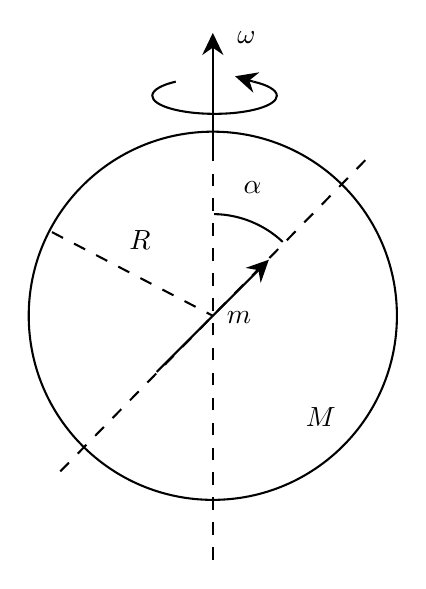
\begin{tikzpicture}[x=0.75pt,y=0.75pt,yscale=-1,xscale=1]
%uncomment if require: \path (0,480); %set diagram left start at 0, and has height of 480

%Shape: Circle [id:dp3694523233703746] 
\draw   (182,222.7) .. controls (182,173.71) and (221.71,134) .. (270.7,134) .. controls (319.69,134) and (359.4,173.71) .. (359.4,222.7) .. controls (359.4,271.69) and (319.69,311.4) .. (270.7,311.4) .. controls (221.71,311.4) and (182,271.69) .. (182,222.7) -- cycle ;
%Straight Lines [id:da307654927906319] 
\draw  [dash pattern={on 4.5pt off 4.5pt}]  (197.2,297.7) -- (344.2,147.7) ;
%Straight Lines [id:da7938927241676892] 
\draw  [dash pattern={on 4.5pt off 4.5pt}]  (270.7,340.2) -- (270.7,105.2) ;
%Straight Lines [id:da18230303159702288] 
\draw [line width=0.75]    (270.7,142.4) -- (270.7,89.4) ;
\draw [shift={(270.7,86.4)}, rotate = 450] [fill={rgb, 255:red, 0; green, 0; blue, 0 }  ][line width=0.08]  [draw opacity=0] (10.72,-5.15) -- (0,0) -- (10.72,5.15) -- (7.12,0) -- cycle    ;
%Straight Lines [id:da02343355138177028] 
\draw  [dash pattern={on 4.5pt off 4.5pt}]  (193.2,182.4) -- (270.7,222.7) ;
%Straight Lines [id:da7072380326449945] 
\draw    (243.7,249.7) -- (295.58,197.82) ;
\draw [shift={(297.7,195.7)}, rotate = 495] [fill={rgb, 255:red, 0; green, 0; blue, 0 }  ][line width=0.08]  [draw opacity=0] (10.72,-5.15) -- (0,0) -- (10.72,5.15) -- (7.12,0) -- cycle    ;
%Shape: Arc [id:dp7695324970163444] 
\draw  [draw opacity=0] (271.29,173.72) .. controls (278.06,173.8) and (284.91,175.29) .. (291.44,178.34) .. controls (296.32,180.62) and (300.65,183.6) .. (304.36,187.11) -- (270.7,222.7) -- cycle ; \draw   (271.29,173.72) .. controls (278.06,173.8) and (284.91,175.29) .. (291.44,178.34) .. controls (296.32,180.62) and (300.65,183.6) .. (304.36,187.11) ;
%Shape: Arc [id:dp00659516312679842] 
\draw  [draw opacity=0] (290.24,109.9) .. controls (297.13,111.5) and (301.54,113.95) .. (301.54,116.71) .. controls (301.54,121.52) and (288.11,125.41) .. (271.54,125.41) .. controls (254.97,125.41) and (241.54,121.52) .. (241.54,116.71) .. controls (241.54,113.95) and (245.95,111.5) .. (252.84,109.9) -- (271.54,116.71) -- cycle ; \draw   (290.24,109.9) .. controls (297.13,111.5) and (301.54,113.95) .. (301.54,116.71) .. controls (301.54,121.52) and (288.11,125.41) .. (271.54,125.41) .. controls (254.97,125.41) and (241.54,121.52) .. (241.54,116.71) .. controls (241.54,113.95) and (245.95,111.5) .. (252.84,109.9) ;
%Straight Lines [id:da20193274094983238] 
\draw    (290.24,109.9) -- (284.32,108.15) ;
\draw [shift={(281.44,107.3)}, rotate = 376.46000000000004] [fill={rgb, 255:red, 0; green, 0; blue, 0 }  ][line width=0.08]  [draw opacity=0] (10.72,-5.15) -- (0,0) -- (10.72,5.15) -- (7.12,0) -- cycle    ;



% Text Node
\draw (229,180.4) node [anchor=north west][inner sep=0.75pt]    {$R$};
% Text Node
\draw (314,265.4) node [anchor=north west][inner sep=0.75pt]    {$M$};
% Text Node
\draw (284,156.4) node [anchor=north west][inner sep=0.75pt]    {$\alpha $};
% Text Node
\draw (276,219.4) node [anchor=north west][inner sep=0.75pt]    {$\ot{m}$};
% Text Node
\draw (281,84.4) node [anchor=north west][inner sep=0.75pt]    {$\omega $};


\end{tikzpicture}
\end{center}

\begin{enumerate}[1)]
  \item Mô tả bức xạ phát ra từ ngôi sao và tính tổng công suất bức xạ của ngôi sao, giả sử rằng góc hợp bởi moment từ và trục quay của ngôi sao là $\alpha$, như trên hình vẽ. 
  \item Tìm độ giảm tốc (hằng số suy giảm đặc trưng của vận tốc góc) của ngôi sao, giả sử rằng năng lượng của ngôi sao chỉ mất mát do bức xạ điện từ.
  \item Giải thích tại sao từ các thông số đã biết như khối lượng, bán kính, chu kì quay $T$, và độ suy giảm $\dd T/ \dd t$ của ngôi sao, chúng ta có thể ước tính được từ trường trên bề mặt ngôi sao. Đưa ra một đáp án bằng số nếu chúng ta biết quan sát và thực nghiệm đã ghi nhận lại được $T= 7,476551 \pm 3 ~\mathrm{s}$ và $\dot{T} = (2,8 \pm 1,4)\times 10^{-11} \approx 10^{-3} ~\mathrm{s/}\text{năm}$ (để đơn giản hóa ta có thể coi $\ot{m}$ là vuông góc với trục quay).

\end{enumerate}
\end{vd}

\begin{loigiai}
\begin{enumerate}[1)]
 \item Vì góc tạo bởi moment từ và trục quay của sao là $\alpha$ khác không, do đó thành phần vuông góc với trục quay của moment $\ot{m}$ sẽ quay với vận tốc góc $\omega$. Do đó, sao Pulsar phát ra bức xạ lưỡng cực có tần số góc $\omega$. Tổng công suất là 
  \[P= \frac{2}{3c^3}\abs{{\ddot{\ot{m}}_{\perp}}}^2 = \frac{2}{3}\dfrac{m_{\perp}^2 \omega^4}{c^3}, \tag{1} \]
ở đây $m_{\perp} = m \sin \alpha $. 
  \item Động năng của hệ là $U= I\omega^2 /2$, ở đây $I= 2MR^2 /5 \approx 1,1\times 10^{43} \,~\mathrm{gcm}^2$ là moment quán tính của ngôi sao trong trường hợp ta giả sử rằng phân bố khối lượng là đều trong toàn hình cầu bán kính $R$. Giả sử năng lượng chỉ mất mát do bức xạ điện từ, ta có 
   \[\frac{\dd U}{\dd t} = \frac{\dd}{\dd t} \left( \frac{I\omega^2}{2}\right)= I\omega\dot{\omega} = -P, \tag{2} \] 
và kết hợp với $1)$ ta có
   \[I\omega \dot{\omega} = - \frac{2}{3} \frac{m_{\perp}^2 \omega^4 }{c^3} \Rightarrow \frac{\dot{\omega}}{\omega^3} = - \frac{2m_{\perp}^2}{3 I c^3}t . \tag{3} \]
Tích phân trên vùng thời gian từ $0$ đến $t$ ta thu được
   \[\frac{1}{2\omega^2(t)} - \frac{1}{2\omega^2(0)} = \frac{2m_{\perp}^2}{3Ic^3} ,\tag{4}\] 

và do đó
   \[\omega(t) =  \frac{\omega(0)}{\sqrt{1+\dfrac{t}{\tau}}}, \ \text{ với } \ \tau = \frac{3Ic^3}{4m_{\perp}^2 \omega^2(0)} . \tag{5} \] 

\item Chúng ta viết lại $\dot{\omega}/\omega^3$ thành $\dot{\omega}/\omega^3 = -T\dot{T}/4\pi^2$, ở đây $T= 2\pi/\omega$ là chu kì quay của Pulsar, và $\dot{T} = -2\pi \dot{\omega}/\omega^2$. Do đó ta thu được moment lưỡng cực $m= m_{\perp}$ như là một hàm của các thông số có được từ thực nghiệm và $2)$:
    \[ m = \sqrt{\frac{3Ic^3}{8\pi^2} T\dot{T}} \approx 3,3 \times 10^{36} \sqrt{T\dot{T}} \,\,~\mathrm{erg/G}, \tag{6} \]

với $T$ được tính theo giây. Cường độ từ trường tức thời trên bề mặt của sao Pulsar tương tự với từ trường gây ra bởi một lưỡng cực từ đặt ở tâm ngôi sao:
     \[\ot{B} = \frac{3({\hat{r}} \cdot \ot{m})\hat{r} - \ot{m}}{r^3}, \tag{7} \]
và dễ thấy $B_{\max} = 2m/R^3$. Thay số ta thu được 
      \[B_{\max} \approx 6,6 \times 10^{21} \sqrt{T\dot{T}} ~ \mathrm{G}, \tag{8} \]
Và kết hợp kết quả thực nghiệm của $T$ và $\dot{T}$ ta thu được 
     \[B_{\max} \approx (9,6\pm 0,25 ) \times 10^{16} ~\mathrm{G}. \tag{9} \]

\end{enumerate}
\end{loigiai}


\begin{vd}[Vòng dây dao động]
Một vòng dây bằng đồng (điện trở rất nhỏ) bán kính $r$, khối lượng $m$ treo bằng một sợi dây thực hiện dao động xoắn với chu kì $T_0$. Cuộn dây có độ tự cảm $L$. Chu kì thay đổi thế nào nếu đặt trong từ trường đồng nhất có cảm ứng từ $\ot{B}$ nằm ngang song song với mặt phẳn vòng dây khi vòng ở vị trí cân bằng. Biết moment quán tính đối với trục đi qua đường kính là $J$.
\begin{center}
    

\tikzset{every picture/.style={line width=0.75pt}} %set default line width to 0.75pt        

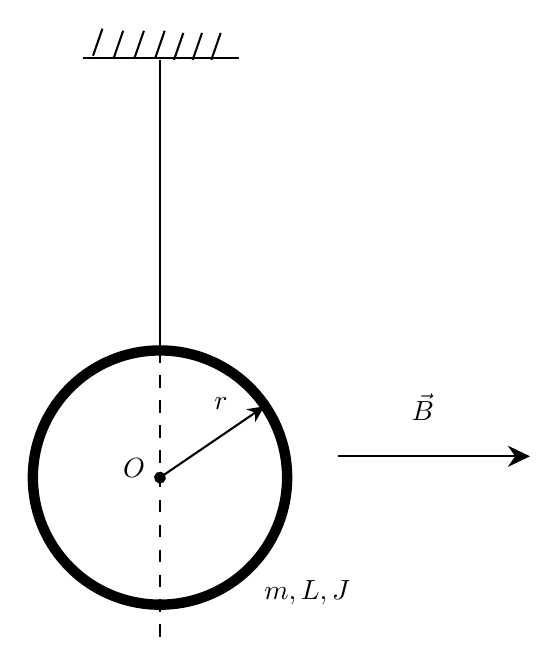
\begin{tikzpicture}[x=0.75pt,y=0.75pt,yscale=-1,xscale=1]
%uncomment if require: \path (0,417); %set diagram left start at 0, and has height of 417

%Shape: Circle [id:dp17346979816986008] 
\draw  [line width=3.75]  (174,252.25) .. controls (174,218.42) and (201.42,191) .. (235.25,191) .. controls (269.08,191) and (296.5,218.42) .. (296.5,252.25) .. controls (296.5,286.08) and (269.08,313.5) .. (235.25,313.5) .. controls (201.42,313.5) and (174,286.08) .. (174,252.25) -- cycle ;
%Straight Lines [id:da552655373957109] 
\draw  [dash pattern={on 4.5pt off 4.5pt}]  (235.25,191) -- (235.25,332) ;
%Straight Lines [id:da3503234546387448] 
\draw    (235.25,51) -- (235.25,191) ;
%Straight Lines [id:da47506307814771076] 
\draw    (198,50) -- (273.5,50) ;
%Straight Lines [id:da9983228801675521] 
\draw    (235.25,252.25) -- (283.02,219.69) ;
\draw [shift={(285.5,218)}, rotate = 505.72] [fill={rgb, 255:red, 0; green, 0; blue, 0 }  ][line width=0.08]  [draw opacity=0] (8.04,-3.86) -- (0,0) -- (8.04,3.86) -- (5.34,0) -- cycle    ;
\draw [shift={(235.25,252.25)}, rotate = 325.72] [color={rgb, 255:red, 0; green, 0; blue, 0 }  ][fill={rgb, 255:red, 0; green, 0; blue, 0 }  ][line width=0.75]      (0, 0) circle [x radius= 2.34, y radius= 2.34]   ;
%Straight Lines [id:da29590519396709736] 
\draw    (203,49) -- (207.5,36) ;
%Straight Lines [id:da8797384501930146] 
\draw    (223,50) -- (227.5,37) ;
%Straight Lines [id:da4152682274694077] 
\draw    (213,50) -- (217.5,37) ;
%Straight Lines [id:da6203719922500526] 
\draw    (242,51) -- (246.5,38) ;
%Straight Lines [id:da6628697806126855] 
\draw    (233,50) -- (237.5,37) ;
%Straight Lines [id:da1980264716128195] 
\draw    (251,51) -- (255.5,38) ;
%Straight Lines [id:da15027155654391278] 
\draw    (260,51) -- (264.5,38) ;
%Straight Lines [id:da3771360602933249] 
\draw    (321,242) -- (410.5,242) ;
\draw [shift={(413.5,242)}, rotate = 180] [fill={rgb, 255:red, 0; green, 0; blue, 0 }  ][line width=0.08]  [draw opacity=0] (10.72,-5.15) -- (0,0) -- (10.72,5.15) -- (7.12,0) -- cycle    ;

% Text Node
\draw (216,241.4) node [anchor=north west][inner sep=0.75pt]    {$O$};
% Text Node
\draw (260,212.4) node [anchor=north west][inner sep=0.75pt]    {$r$};
% Text Node
\draw (284,300.4) node [anchor=north west][inner sep=0.75pt]    {$m,L,J$};
% Text Node
\draw (355,210.4) node [anchor=north west][inner sep=0.75pt]    {$\vec{B}$};


\end{tikzpicture}

\end{center}
\end{vd}
\begin{loigiai}
Về biến dạng xoắn, ta sẽ gọi hệ số tỉ lệ là $A$, ta thu được phương tình vi phân dao động do biến dạng xoắn: $A\theta=-J\ddot{\theta}$.\\
Từ đó chu kì:
$$T_0=2\pi\sqrt{\dfrac{J}{A}}$$
Khi có từ trường, từ thông xuyên qua vòng khi vòng xê dịch một góc nhỏ là:
$$\Phi=BS\cdot \mathrm{sin}\theta \approx BS\theta$$
Suất điện động tự cảm đúng bằng suất điện động cảm ứng sinh ra trên vòng:
$$L\cdot\dfrac{\mathrm{d}i}{\mathrm{d}t}=BS\cdot\dfrac{\mathrm{d}\theta}{\mathrm{d}t} \Rightarrow Li=BS\theta + C$$
Khi $i=0$ thì $\theta=0$ nên hằng số $C=0 \Rightarrow i=BS\theta/L$.\\
Moment từ: $\ot{M}=\ot{p_m}\times\ot{B}=iSB \approx B^2S^2\theta/L$.
Ta có phương trình vi phân dạng mới:
$$-\dfrac{B^2S^2}{L}\theta-A\theta=J\ddot{\theta}\Leftrightarrow \left(-\dfrac{B^2S^2}{L}-\dfrac{4\pi^2J}{T_0^2}\right)\theta=J\ddot{\theta}$$
Chu kì dao động mới:
$$T=\dfrac{T_0}{\sqrt{\dfrac{B^2S^2T_0^2}{4\pi^2JL}+1}}.$$
\end{loigiai}


\begin{vd}[Bước vào từ trường]
Hãy xét một từ trường đều $B$ trong vùng màu xám và hướng ra ngoài mặt phẳng hình vẽ, như các hình dưới đây.
\begin{center}
    

\tikzset{every picture/.style={line width=0.75pt}} %set default line width to 0.75pt        

\begin{tikzpicture}[x=0.75pt,y=0.75pt,yscale=-1,xscale=1]
%uncomment if require: \path (0,300); %set diagram left start at 0, and has height of 300

%Shape: Rectangle [id:dp751914180106541] 
\draw  [color={rgb, 255:red, 155; green, 155; blue, 155 }  ,draw opacity=1 ][fill={rgb, 255:red, 155; green, 155; blue, 155 }  ,fill opacity=1 ] (33,128.63) -- (193.75,128.63) -- (193.75,213.06) -- (33,213.06) -- cycle ;
%Shape: Rectangle [id:dp5715554387472597] 
\draw  [color={rgb, 255:red, 155; green, 155; blue, 155 }  ,draw opacity=1 ][fill={rgb, 255:red, 155; green, 155; blue, 155 }  ,fill opacity=1 ] (233.1,109) -- (393.85,109) -- (393.85,193.43) -- (233.1,193.43) -- cycle ;
%Shape: Rectangle [id:dp4433680938904905] 
\draw  [color={rgb, 255:red, 155; green, 155; blue, 155 }  ,draw opacity=1 ][fill={rgb, 255:red, 155; green, 155; blue, 155 }  ,fill opacity=1 ] (430.69,144.83) -- (532,144.83) -- (532,212.12) -- (430.69,212.12) -- cycle ;
%Curve Lines [id:da7432949283072408] 
\draw    (101.34,158.57) .. controls (135.22,158.57) and (128.91,184.65) .. (126.04,190.52) ;
%Straight Lines [id:da15327337471065383] 
\draw    (97.32,157.91) -- (101.34,158.57) ;
%Straight Lines [id:da9237701245729204] 
\draw    (97.32,157.91) -- (95.6,164.43) ;
%Curve Lines [id:da846544871091409] 
\draw    (95.6,164.43) .. controls (88.71,170.3) and (89.28,178.13) .. (87.47,184.05) .. controls (85.66,189.97) and (82.97,186.61) .. (97.9,189.22) ;
%Curve Lines [id:da3612566481757702] 
\draw    (97.9,189.22) .. controls (99.05,202.91) and (92.73,204.87) .. (117.42,194.44) ;
%Straight Lines [id:da9634504850992611] 
\draw    (126.04,190.52) -- (117.42,194.44) ;

%Curve Lines [id:da7805941099664069] 
\draw    (305.63,178.19) .. controls (339.51,178.19) and (333.2,204.28) .. (330.32,210.15) ;
%Straight Lines [id:da4463686851471427] 
\draw    (301.61,177.54) -- (305.63,178.19) ;
%Straight Lines [id:da4213043294347989] 
\draw    (301.61,177.54) -- (299.89,184.06) ;
%Curve Lines [id:da8307231428150825] 
\draw    (299.89,184.06) .. controls (293,189.93) and (293.57,197.76) .. (291.76,203.68) .. controls (289.95,209.6) and (287.25,206.24) .. (302.19,208.85) ;
%Curve Lines [id:da4478446011588786] 
\draw    (302.19,208.85) .. controls (303.33,222.54) and (297.02,224.5) .. (321.71,214.06) ;
%Straight Lines [id:da9224516498692135] 
\draw    (330.32,210.15) -- (321.71,214.06) ;

%Shape: Chord [id:dp3024926209068406] 
\draw   (511.73,185.21) .. controls (512.95,188.32) and (513.6,191.68) .. (513.58,195.2) .. controls (513.49,210.68) and (500.3,223.14) .. (484.12,223.02) .. controls (467.93,222.91) and (454.88,210.26) .. (454.97,194.78) .. controls (454.99,191.27) and (455.69,187.91) .. (456.94,184.82) -- cycle ;
%Straight Lines [id:da2851947683889342] 
\draw  [dash pattern={on 0.84pt off 2.51pt}]  (297.22,194.05) -- (328.9,194.05) ;
\draw [shift={(331.9,194.05)}, rotate = 180] [fill={rgb, 255:red, 0; green, 0; blue, 0 }  ][line width=0.08]  [draw opacity=0] (10.72,-5.15) -- (0,0) -- (10.72,5.15) -- (7.12,0) -- cycle    ;
\draw [shift={(294.22,194.05)}, rotate = 0] [fill={rgb, 255:red, 0; green, 0; blue, 0 }  ][line width=0.08]  [draw opacity=0] (8.93,-4.29) -- (0,0) -- (8.93,4.29) -- cycle    ;
%Straight Lines [id:da6949611555798287] 
\draw  [dash pattern={on 0.84pt off 2.51pt}]  (475.07,185.33) -- (475.07,212.43) ;


% Text Node
\draw (51.95,135.52) node [anchor=north west][inner sep=0.75pt]   [align=left] {vùng từ trường $\displaystyle B$};
% Text Node
\draw (251.21,114.95) node [anchor=north west][inner sep=0.75pt]   [align=left] {vùng từ trường $\displaystyle B$};
% Text Node
\draw (307.48,195.68) node [anchor=north west][inner sep=0.75pt]  [font=\scriptsize]  {$w$};
% Text Node
\draw (478.28,195.68) node [anchor=north west][inner sep=0.75pt]  [font=\scriptsize]  {$y$};
% Text Node
\draw (99.11,235.05) node [anchor=north west][inner sep=0.75pt]    {$( 1)$};
% Text Node
\draw (300.89,233.18) node [anchor=north west][inner sep=0.75pt]    {$( 2)$};
% Text Node
\draw (474.2,233.18) node [anchor=north west][inner sep=0.75pt]    {$( 3)$};


\end{tikzpicture}
\end{center}
\begin{enumerate}[1)]%tutruong (0)
    \item Tìm lực do từ trường tác dụng lên một cuộn dây dẫn mảnh khép kín mang theo một dòng điện không đổi $I$, tất cả cuộn dây dẫn nằm bên trong vùng từ trường. Mặt phẳng cuộn dây nằm trong mặt phẳng hình vẽ. 
    \item Lực do từ trường tác dụng lên cuộn dây dẫn khi một phần của nó nằm ngoài vùng có từ trường có thể được viết dưới dạng $F=\alpha wBI$, trong đó $w$ là khoảng cách giữa hai điểm của cuộn dây cắt cạnh đáy của vùng từ trường, và hướng của nó là một trong hai hướng: lên hoặc xuống tùy thuộc vào chiều của dòng điện. Tìm giá trị của $\alpha$.
    \item Cho một cuộn dây mảnh hình bán nguyệt $r$, điện trở $R$, và khối lượng $m$ rơi xuống và đi ra ngoài vùng từ trường. Mặt phẳng của cuộn dây nằm trong mặt phẳng tờ giấy, và cạnh thẳng của vòng dây song song với cạnh đáy nằm ngang của vùng từ trường. Bỏ qua hiện tượng tự cảm của cuộn dây. Viết phương trình vi phân cho $y (<r)$ là khoảng cách giữa cạnh thẳng của cuộn dây và cạnh đáy của vùng từ trường. Nếu bạn chưa tìm thấy $\alpha$ trong ý $(2)$. Bạn có thể sử dụng nó như một hằng số đã biết để giải ý $(3)$.
\end{enumerate}
\end{vd}
\begin{loigiai}
\begin{enumerate}[1)]
    \item 
\begin{enumerate}[\text{Câu trả lời} 1:]
    \item Cuộn dây là tổng của rất nhiều cuộn dây nhỏ hình vuông. Lực từ tác dụng lên từng cuộn dây nhỏ bằng không, do đó hợp lực tác dụng lên vòng dây bằng không. 
    \item Di chuyển cuộn dây trong một từ trường không cần thực hiện công, do không có hiện tượng cảm ứng điện từ, do đó hợp lực bằng không.
    \item Sử dụng hình chiếu của vector.
\end{enumerate}
    \item Cuộn dây được chia làm hai nửa tại ranh giới của từ trường, giả sử có một dòng dương và một dòng âm.\\$\alpha=1$
    \item Di chuyển cuộn dây trong từ trường, cắt các đường sức từ trường
    \[w=2\sqrt{r^2-y^2},\]
    kết quả là dòng điện được tạo ra
    \[I=\dfrac{Bwv}{R}.\]
    trong đó $v=-\dfrac{\mathrm{d}y}{\mathrm{d}t}$ (do $y$ giảm và $v$ tăng.)\\
    Lực từ tác dụng lên cuộn dây $F=IBw$.\\
    Phương trình chuyển động
    \[m\dfrac{\mathrm{d}^2y}{\mathrm{d}t^2}=F-mg.\]
    Kết hợp tất cả các phương trình trên lại ta được
    \[\dfrac{\mathrm{d}^2y}{\mathrm{d}t}+\dfrac{4B^2}{mR}(r^2-y^2)\dfrac{\mathrm{d}y}{\mathrm{d}t}+g=0.\]
\end{enumerate}
\end{loigiai}



\begin{vd}[Điện tích điểm trong từ trường]
Một điện tích điểm $-q(q>0)$ khối lượng $m$ chuyển động không ma sát trong một miền có từ trường được cho bởi biểu thức $\ot{B}=B_0\dfrac{a}{r}\ot{z} (B_0>0)$ với $r=\sqrt{x^2+y^2}$ là khoảng cách tính từ trục $z$. Tại thời điểm $t=0$, vị trí và vận tốc ban đầu của điện tích là $(x=a,y=0,z=0)$ và $(v_{x}=a,v_{y}=v_0,v_{z}=0)$, ở đây $a$, $v_0>0$.
\begin{enumerate}[1) ]
    \item Chứng minh rằng hạt luôn nằm trên mặt phẳng $xy$.
    \item Tìm vận tốc ban đầu, mà với vận tốc đó điện tích có thể thực hiện một chuyển động tròn xung quanh gốc tọa độ. 
    \item Bây giờ vận tốc ban đầu không bằng với câu trả lời trong ý $(2)$. Thiết lập phương trình vi phân dưới dạng $\dfrac{\mathrm{d}L}{\mathrm{d}r}=\const$, với $L$ là moment động lượng của điện tích đối với trục $z$, và giải phương trình vi phân đó. Nếu bạn không thể xác định được hằng số đó, bạn hãy giả sử rằng hằng số đó đã biết và giải các ý $(4)$ và $(5)$.\\
    (\textit{Gợi ý:} $\ot{A}\times(\ot{C}\times\ot{B})=(\ot{A}\cdot\ot{B})\cdot\ot{C}-(\ot{A}\cdot\ot{C})\cdot\ot{B}$) 
    \item Từ kết quả của ý $(3)$, hãy tìm khoảng cách từ điện tích tới gốc tọa độ khi mà nó chuyển động theo phương tiếp tuyến với quỹ đạo $(\ot{v}\bot \ot{r})$. Tìm vận tốc nhỏ nhất $v_0$ mà điện tích không bao giờ có thể dịch chuyển theo phương tiếp tuyến sau khi nó được cung cấp vận tốc.
    \item Tìm khoảng cách tính từ gốc khi điện tích đang chuyển động theo hướng xuyên tâm ($\ot{v}$ song song với $\ot{r}$). Tìm vận tốc nhỏ nhất $v_0$ mà điện tích không bao giờ có thể dịch chuyển theo phương xuyên tâm sau khi nó được cung cấp vận tốc.
\end{enumerate}
\end{vd}
\begin{loigiai}
\begin{enumerate}[1) ]
    \item  Theo định luật lực Lorentz $\ot{F}=-q\ot{v}\times\ot{B}$, lực $F$ không có thành phần dọc theo trục $z$ vì từ trường $\ot{B}$ hướng dọc theo trục $z$. Do đó, nếu vận tốc ban đầu $v_{z}=0$ thì điện tích luôn chuyển động trong mặt phẳng $x-y$. 
    \item Từ trường $B$ tại $r=a$ là vừa đủ để hạt chuyển động trên một quỹ đạo tròn bán kính $a$.
    \[\dfrac{mv_0^2}{a}=qv_0B_0\rt v_0=\dfrac{qB_0a}{m}.\]
    \item Gọi moment động lượng của điện tích đối với gốc là $L$. Khi đó $L(t=0)=mv_0a$. Ta có
    \begin{align*}
        \dfrac{\mathrm{d}L}{\mathrm{d}t}&=-rF\mathrm{\sin{\theta}}\\
        &=-qrvB\mathrm{\cos{\phi}}\\
        &=-qrBv_{r}=qrB\dfrac{\mathrm{d}r}{\mathrm{d}t}\\
        \Longleftrightarrow\dfrac{\mathrm{d}L}{\mathrm{d}r}&=qrB.
    \end{align*}
    với $v_{r}=\dfrac{\mathrm{d}r}{\mathrm{d}t}$ là vận tốc theo phương xuyên tâm.\\
    \begin{center}
        

\tikzset{every picture/.style={line width=0.75pt}} %set default line width to 0.75pt        

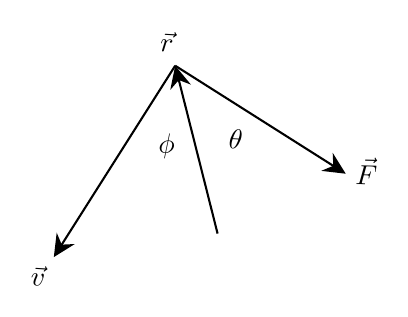
\begin{tikzpicture}[x=0.75pt,y=0.75pt,yscale=-1,xscale=1]
%uncomment if require: \path (0,300); %set diagram left start at 0, and has height of 300

%Straight Lines [id:da6526384579910471] 
\draw    (308.37,81.97) -- (388.02,132.42) ;
\draw [shift={(390.55,134.02)}, rotate = 212.35] [fill={rgb, 255:red, 0; green, 0; blue, 0 }  ][line width=0.08]  [draw opacity=0] (10.72,-5.15) -- (0,0) -- (10.72,5.15) -- (7.12,0) -- cycle    ;
%Straight Lines [id:da8692651038771895] 
\draw    (308.37,81.97) -- (251.5,171.65) ;
\draw [shift={(249.89,174.19)}, rotate = 302.38] [fill={rgb, 255:red, 0; green, 0; blue, 0 }  ][line width=0.08]  [draw opacity=0] (10.72,-5.15) -- (0,0) -- (10.72,5.15) -- (7.12,0) -- cycle    ;
%Straight Lines [id:da5723833940518483] 
\draw    (328.79,162.84) -- (309.11,84.88) ;
\draw [shift={(308.37,81.97)}, rotate = 435.83000000000004] [fill={rgb, 255:red, 0; green, 0; blue, 0 }  ][line width=0.08]  [draw opacity=0] (10.72,-5.15) -- (0,0) -- (10.72,5.15) -- (7.12,0) -- cycle    ;


% Text Node
\draw (237.8,176.73) node [anchor=north west][inner sep=0.75pt]  [font=\normalsize,rotate=-3.57]  {$\vec{v}$};
% Text Node
\draw (393.99,124.83) node [anchor=north west][inner sep=0.75pt]  [font=\normalsize,rotate=-1.42]  {$\vec{F}$};
% Text Node
\draw (300.05,64.15) node [anchor=north west][inner sep=0.75pt]  [font=\normalsize,rotate=-3.17]  {$\vec{r}$};
% Text Node
\draw (333.11,110.86) node [anchor=north west][inner sep=0.75pt]  [font=\normalsize,rotate=-3.37]  {$\theta $};
% Text Node
\draw (298.46,113.41) node [anchor=north west][inner sep=0.75pt]  [font=\normalsize,rotate=-357.66]  {$\phi $};


\end{tikzpicture}
    \end{center}
    Chúng ta cũng có thể tìm được phương trình vi phân bằng cách
    \[\dfrac{\mathrm{d}\ot{L}}{\mathrm{d}t}=\ot{r}\times\ot{F}=-q\ot{r}\times(\ot{v}\times\ot{B})=-q\left((\ot{r}\cdot\ot{B})\cdot\ot{v}-(\ot{r}\cdot\ot{v})\cdot\ot{B}\right)=qrv_{r}\ot{B}=qr\dfrac{\mathrm{d}r}{\mathrm{d}t}\ot{B}.\]
    Suy ra
    \begin{align*}
       \dfrac{\mathrm{d}\ot{L}}{\mathrm{d}t} &=qrB\dfrac{\mathrm{d}r}{\mathrm{d}t}\\
       \dfrac{\mathrm{d}\ot{L}}{\mathrm{d}r} &=qrB\\
        \Leftrightarrow L(r)-L(a)&=\int_{a}^{r}qBr\mathrm{d}r=qB_0a(r-a).
    \end{align*} 
    \item Bởi vì từ trường $B$ không hoạt động, vận tốc của điện tích luôn luôn là $v_0$. Lưu ý moment động lượng có thể là $L=\pm mrv_0$.\\
    Khi $L=mrv_0$, $r=a$, không có chuyển động theo phương tiếp tuyến ngay sau đó.\\
    Khi $L=-mrv_0$
    \[r=a\dfrac{qB_0a-mv_0}{qB_0a+mv_0}.\]
    Khi $qB_0a<mv_0$, nghiệm duy nhất của phương trình là $r=a$, tương ứng với các điều kiện ban đầu. Không có chuyển động theo phương tiếp tuyến xảy ra ngay sau đó.\\
    Khi $qB_0a>mv_0$,
    \[r=a\dfrac{qB_0a-mv_0}{qB_0a+mv_0}<a.\]
    điều đó là có thể xảy ra.
    \item Khi điện tích chuyển động theo phương xuyên tâm, thì $L=0$, do đó
    \[r=a\left(1-\dfrac{mv_0}{qB_0a}\right).\]
    Khi $qB_0a>mv_0$, $r>0$, chuyển động có thể hướng tâm.\\
    Khi $qB_0a<mv_0$, $r<0$, chuyển động sẽ không bao giờ là hướng tâm.
\end{enumerate}
\end{loigiai}


\begin{vd}[Quay trong lòng Solenoid]
Một đĩa kim loại bán kính $r$ có thể quay với ma sát không đáng kể bên trong một cuộn dây dài, thẳng, quanh một trục song song với trục đối xứng của cuộn dây. Một đầu của cuộn dây được nối với cạnh của đĩa còn đầu kia nối với trục. Cuộn dây có điện trở $R$ và chứa $n$ vòng trên mỗi đơn vị chiều dài, được đặt sao cho trục của nó song song với vector cảm ứng từ $\ot{B_0}$ của Trái Đất.

\begin{center}
    

\tikzset{every picture/.style={line width=0.75pt}} %set default line width to 0.75pt        

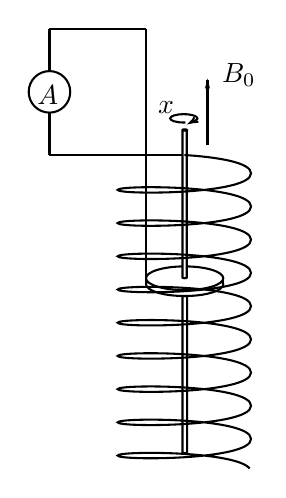
\begin{tikzpicture}[x=0.75pt,y=0.75pt,yscale=-1,xscale=1,scale=0.4]
%uncomment if require: \path (0,725); %set diagram left start at 0, and has height of 725

%Shape: Can [id:dp794933563146212] 
\draw  [fill={rgb, 255:red, 255; green, 255; blue, 255 }  ,fill opacity=1 ] (388.83,324.64) -- (388.83,513.93) .. controls (388.83,514.39) and (387.58,514.77) .. (386.04,514.77) .. controls (384.5,514.77) and (383.25,514.39) .. (383.25,513.93) -- (383.25,324.64) .. controls (383.25,324.18) and (384.5,323.8) .. (386.04,323.8) .. controls (387.58,323.8) and (388.83,324.18) .. (388.83,324.64) .. controls (388.83,325.1) and (387.58,325.48) .. (386.04,325.48) .. controls (384.5,325.48) and (383.25,325.1) .. (383.25,324.64) ;
%Shape: Ellipse [id:dp9073150731380437] 
\draw  [fill={rgb, 255:red, 255; green, 255; blue, 255 }  ,fill opacity=1 ] (339.33,311.08) .. controls (339.33,303.2) and (360.15,296.8) .. (385.83,296.8) .. controls (411.51,296.8) and (432.33,303.2) .. (432.33,311.08) .. controls (432.33,318.96) and (411.51,325.35) .. (385.83,325.35) .. controls (360.15,325.35) and (339.33,318.96) .. (339.33,311.08) -- cycle ;
%Shape: Ellipse [id:dp7831632242132669] 
\draw  [fill={rgb, 255:red, 255; green, 255; blue, 255 }  ,fill opacity=1 ] (339.33,303.94) .. controls (339.33,296.06) and (360.15,289.67) .. (385.83,289.67) .. controls (411.51,289.67) and (432.33,296.06) .. (432.33,303.94) .. controls (432.33,311.83) and (411.51,318.22) .. (385.83,318.22) .. controls (360.15,318.22) and (339.33,311.83) .. (339.33,303.94) -- cycle ;
%Straight Lines [id:da15211630183630298] 
\draw [fill={rgb, 255:red, 255; green, 255; blue, 255 }  ,fill opacity=1 ]   (339.33,302.86) -- (339.33,311.08) ;
%Straight Lines [id:da4152297399713436] 
\draw    (432.33,303.94) -- (432.33,311.08) ;

%Shape: Can [id:dp6293113679467115] 
\draw  [fill={rgb, 255:red, 255; green, 255; blue, 255 }  ,fill opacity=1 ] (388.33,125.29) -- (388.33,303.18) .. controls (388.33,303.6) and (387.2,303.94) .. (385.79,303.94) .. controls (384.39,303.94) and (383.25,303.6) .. (383.25,303.18) -- (383.25,125.29) .. controls (383.25,124.87) and (384.39,124.53) .. (385.79,124.53) .. controls (387.2,124.53) and (388.33,124.87) .. (388.33,125.29) .. controls (388.33,125.71) and (387.2,126.05) .. (385.79,126.05) .. controls (384.39,126.05) and (383.25,125.71) .. (383.25,125.29) ;
%Shape: Spring [id:dp8083999628893139] 
\draw   (385.48,155.53) .. controls (425.64,158.03) and (465.79,164.53) .. (465.79,177.53) .. controls (465.79,203.53) and (305.16,203.53) .. (305.16,197.53) .. controls (305.16,191.53) and (465.79,191.53) .. (465.79,217.53) .. controls (465.79,243.53) and (305.16,243.53) .. (305.16,237.53) .. controls (305.16,231.53) and (465.79,231.53) .. (465.79,257.53) .. controls (465.79,283.53) and (305.16,283.53) .. (305.16,277.53) .. controls (305.16,271.53) and (465.79,271.53) .. (465.79,297.53) .. controls (465.79,323.53) and (305.16,323.53) .. (305.16,317.53) .. controls (305.16,311.53) and (465.79,311.53) .. (465.79,337.53) .. controls (465.79,363.53) and (305.16,363.53) .. (305.16,357.53) .. controls (305.16,351.53) and (465.79,351.53) .. (465.79,377.53) .. controls (465.79,403.53) and (305.16,403.53) .. (305.16,397.53) .. controls (305.16,391.53) and (465.79,391.53) .. (465.79,417.53) .. controls (465.79,443.53) and (305.16,443.53) .. (305.16,437.53) .. controls (305.16,431.53) and (465.79,431.53) .. (465.79,457.53) .. controls (465.79,483.53) and (305.16,483.53) .. (305.16,477.53) .. controls (305.16,471.53) and (465.79,471.53) .. (465.79,497.53) .. controls (465.79,523.53) and (305.16,523.53) .. (305.16,517.53) .. controls (305.16,511.89) and (446.83,511.55) .. (464.08,533.06) ;
%Straight Lines [id:da16873648988922163] 
\draw    (222.33,155.53) -- (384.33,155.53) ;

%Straight Lines [id:da34653262474759705] 
\draw    (339.33,3.38) -- (339.33,311.08) ;
%Straight Lines [id:da14719050864648686] 
\draw    (223,3.38) -- (339.33,3.38) ;
%Straight Lines [id:da9406743709845233] 
\draw    (223,3.38) -- (223,155.53) ;
%Shape: Circle [id:dp46030588478741774] 
\draw  [fill={rgb, 255:red, 255; green, 255; blue, 255 }  ,fill opacity=1 ] (198,79.45) .. controls (198,65.64) and (209.19,54.45) .. (223,54.45) .. controls (236.81,54.45) and (248,65.64) .. (248,79.45) .. controls (248,93.26) and (236.81,104.45) .. (223,104.45) .. controls (209.19,104.45) and (198,93.26) .. (198,79.45) -- cycle ;
%Straight Lines [id:da19632157276818174] 
\draw    (413.33,143.38) -- (413.33,65.38) ;
\draw [shift={(413.33,63.38)}, rotate = 450] [fill={rgb, 255:red, 0; green, 0; blue, 0 }  ][line width=0.08]  [draw opacity=0] (12,-3) -- (0,0) -- (12,3) -- cycle    ;
%Shape: Arc [id:dp5146791024977042] 
\draw  [draw opacity=0] (386.58,116.33) .. controls (385.99,116.35) and (385.38,116.36) .. (384.77,116.36) .. controls (375.69,116.36) and (368.33,114.11) .. (368.33,111.34) .. controls (368.33,108.58) and (375.69,106.33) .. (384.77,106.33) .. controls (393.85,106.33) and (401.21,108.58) .. (401.21,111.34) .. controls (401.21,113.22) and (397.83,114.85) .. (392.83,115.71) -- (384.77,111.34) -- cycle ; \draw   (386.58,116.33) .. controls (385.99,116.35) and (385.38,116.36) .. (384.77,116.36) .. controls (375.69,116.36) and (368.33,114.11) .. (368.33,111.34) .. controls (368.33,108.58) and (375.69,106.33) .. (384.77,106.33) .. controls (393.85,106.33) and (401.21,108.58) .. (401.21,111.34) .. controls (401.21,113.22) and (397.83,114.85) .. (392.83,115.71) ;
\draw   (402.4,115.67) .. controls (398.49,115.4) and (395.13,115.75) .. (392.33,116.71) .. controls (394.59,115.14) and (396.28,112.94) .. (397.44,110.14) ;



% Text Node
\draw (204.67,68) node [anchor=north west][inner sep=0.75pt]  [font=\normalsize] [align=left] {$A$};
% Text Node
\draw (427.33,41.44) node [anchor=north west][inner sep=0.75pt]  [font=\normalsize]  {$\ot{B_{0}}$};
% Text Node
\draw (350,87.4) node [anchor=north west][inner sep=0.75pt]  [font=\normalsize]  {$x$};


\end{tikzpicture}

\end{center}
Hỏi cường độ dòng điện chạy qua Ampe kế bằng bao nhiêu nếu đĩa quay với tốc độ góc  $\omega$. Hãy vẽ đồ thị biểu diễn sự phụ thuộc của cường độ dòng điện $I$ vào vận tốc góc  $\omega$ (đối với cả giá trị âm và dương của  $\omega$). Hãy chứng minh rằng công suất cần thiết để quay đĩa bằng công suất tỏa nhiệt trong cuộn dây.
\end{vd}
\begin{loigiai}
Từ trường tổng hợp $B’$ là tổng của từ trường Trái Đất và từ trường do cuộn dây gây ra, tương ứng với $B_0$ và $B$, tức là
\[ B'=B_0\pm B. \tag{1} \label{pt1}\]
Dòng điện chạy qua cuộn dây được xác định bởi suất điện động cảm ứng $V_i$ và điện trở $R$,
	\[I=\dfrac{V_i}{R}=B'\dfrac{r^2\omega}{2}\dfrac{1}{R}, \tag{2}
	\label{pt2}\]
trong đó suất điện động cảm ứng được tính từ tốc độ biến thiên từ thông. Từ trường gây ra bởi cuộn dây là
	\[ B=\mu_0nI. \tag{3}
	\label{pt3}\] 
Từ ba phương trình trên, có thể dễ dàng tính được $B$, $B’$ và $I$. Hai dấu (+) và ($-$) trong phương trình (\ref{pt1}) phù hợp với cả giá trị âm và dương của tần số góc. Giá trị của  $\omega$ được lấy là dương nếu từ trường do cuộn dây tạo ra cùng hướng với từ trường Trái Đất. Thu được các kết quả sau của từ trường tổng hợp và cường độ dòng điện:
\[ B'=\dfrac{2R{B_0}}{2R-\mu_0n{r^2}\omega},\] 
và 
\[ I=\dfrac{B_0r^2\omega}{2R-\mu_0n{r^2}\omega}.\]
Như mong đợi, khi đĩa ở trạng thái nghỉ, cường độ dòng điện bằng $0$ và từ trường tổng hợp bên trong cuộn dây chỉ đơn giản là $B_0$, đúng bằng từ trường Trái Đất.\\
Khi đĩa quay sao cho từ trường do cuộn dây gây ra ngược chiều với từ trường của Trái Đất ($\omega$ < 0), từ trường tổng hợp sẽ giảm tiệm cận về $0$ khi tần số góc của đĩa (âm) tăng. Ở tốc độ quay cao như vậy, dòng điện chạy trong cuộn dây có giá trị $\dfrac{-B_0}{{\mu_0}n}$ (giá trị cần thiết để triệt tiêu từ trường Trái Đất).\\
Xoay đĩa theo hướng ngược lại, ($\omega$ > 0), làm cho từ trường tổng hợp tăng lên, tạo ra suất điện động lớn hơn, khiến cho dòng điện cũng lớn hơn, từ đó dẫn đến sự gia tăng hơn nữa của từ trường. Dưới các điều kiện thuận lợi này, cả từ trường và cường độ dòng điện cùng tiến tới vô cùng khi tần số góc có một giá trị “đặc biệt” 
$4\omega_{\text{tới hạn}}=\dfrac{2R}{\left(\mu_0n{r^2}\right)}$, như trong hình \ref{ng.h1}. Một trạng thái như vậy rõ ràng là không thể đạt được trong thực tế. Nếu tần số góc tăng quá nhiều, dòng điện và nhiệt được cung cấp bởi cuộn dây sẽ tăng cho đến khi dây bị cháy!
\begin{figure}[h!]
    \centering
    \begin{subfigure}{0.45\textwidth}
    \centering
    

\tikzset{every picture/.style={line width=0.75pt}} %set default line width to 0.75pt        

\begin{tikzpicture}[x=0.75pt,y=0.75pt,yscale=-1,xscale=1]
%uncomment if require: \path (0,292); %set diagram left start at 0, and has height of 292

%Straight Lines [id:da5377020320512023] 
\draw    (284.6,246.93) -- (284.6,65.13) ;
\draw [shift={(284.6,62.13)}, rotate = 450] [fill={rgb, 255:red, 0; green, 0; blue, 0 }  ][line width=0.08]  [draw opacity=0] (10.72,-5.15) -- (0,0) -- (10.72,5.15) -- (7.12,0) -- cycle    ;
%Straight Lines [id:da16274924439367822] 
\draw    (224.6,185.73) -- (411.2,185.73) ;
\draw [shift={(414.2,185.73)}, rotate = 180] [fill={rgb, 255:red, 0; green, 0; blue, 0 }  ][line width=0.08]  [draw opacity=0] (10.72,-5.15) -- (0,0) -- (10.72,5.15) -- (7.12,0) -- cycle    ;
%Straight Lines [id:da5900321071455628] 
\draw  [dash pattern={on 4.5pt off 4.5pt}]  (343.2,61.33) -- (343.2,246.53) ;
%Curve Lines [id:da23607602398826577] 
\draw    (227,180.93) .. controls (295.8,170.53) and (349,159.73) .. (340.2,65.33) ;
%Curve Lines [id:da053888858283025254] 
\draw    (348.2,243.73) .. controls (350.6,209.33) and (361,188.93) .. (401,186.93) ;
%Flowchart: Connector [id:dp8556368316050571] 
\draw  [fill={rgb, 255:red, 0; green, 0; blue, 0 }  ,fill opacity=1 ] (282,168.23) .. controls (282,166.96) and (283.03,165.93) .. (284.3,165.93) .. controls (285.57,165.93) and (286.6,166.96) .. (286.6,168.23) .. controls (286.6,169.5) and (285.57,170.53) .. (284.3,170.53) .. controls (283.03,170.53) and (282,169.5) .. (282,168.23) -- cycle ;
%Flowchart: Connector [id:dp3958596104050942] 
\draw  [fill={rgb, 255:red, 0; green, 0; blue, 0 }  ,fill opacity=1 ] (340.8,184.63) .. controls (340.8,183.36) and (341.83,182.33) .. (343.1,182.33) .. controls (344.37,182.33) and (345.4,183.36) .. (345.4,184.63) .. controls (345.4,185.9) and (344.37,186.93) .. (343.1,186.93) .. controls (341.83,186.93) and (340.8,185.9) .. (340.8,184.63) -- cycle ;

% Text Node
\draw (259.2,146.93) node [anchor=north west][inner sep=0.75pt]    {$B_{0}$};
% Text Node
\draw (281.2,40.13) node [anchor=north west][inner sep=0.75pt]    {$B'$};
% Text Node
\draw (346.8,166.93) node [anchor=north west][inner sep=0.75pt]    {$\text{tới hạn}$};


\end{tikzpicture}

    \caption{}
    \end{subfigure}
    \begin{subfigure}{0.45\textwidth}
    \centering
    

\tikzset{every picture/.style={line width=0.75pt}} %set default line width to 0.75pt        

\begin{tikzpicture}[x=0.75pt,y=0.75pt,yscale=-1,xscale=1]
%uncomment if require: \path (0,292); %set diagram left start at 0, and has height of 292

%Straight Lines [id:da22702238602532332] 
\draw    (281,231.73) -- (281,23.53) ;
\draw [shift={(281,20.53)}, rotate = 450] [fill={rgb, 255:red, 0; green, 0; blue, 0 }  ][line width=0.08]  [draw opacity=0] (10.72,-5.15) -- (0,0) -- (10.72,5.15) -- (7.12,0) -- cycle    ;
%Straight Lines [id:da5449001013666472] 
\draw    (212.2,142.33) -- (427.6,142.33) ;
\draw [shift={(430.6,142.33)}, rotate = 180] [fill={rgb, 255:red, 0; green, 0; blue, 0 }  ][line width=0.08]  [draw opacity=0] (10.72,-5.15) -- (0,0) -- (10.72,5.15) -- (7.12,0) -- cycle    ;
%Curve Lines [id:da7937706081551041] 
\draw    (216.2,157.33) .. controls (253.8,153.73) and (306.6,137.73) .. (325.8,116.13) .. controls (345,94.53) and (347,73.73) .. (345,25.73) ;
%Straight Lines [id:da1914924121278221] 
\draw  [dash pattern={on 4.5pt off 4.5pt}]  (348.2,20.53) -- (348.6,232.93) ;
%Straight Lines [id:da5765469163981802] 
\draw  [dash pattern={on 0.84pt off 2.51pt}]  (211,161.53) -- (424.6,161.53) ;
%Curve Lines [id:da7040009088385004] 
\draw    (352.6,230.53) .. controls (357.4,187.73) and (368.2,168.53) .. (415,164.13) ;
%Shape: Circle [id:dp9722098315972509] 
\draw  [fill={rgb, 255:red, 0; green, 0; blue, 0 }  ,fill opacity=1 ] (279,142.1) .. controls (279,140.83) and (280.03,139.8) .. (281.3,139.8) .. controls (282.57,139.8) and (283.6,140.83) .. (283.6,142.1) .. controls (283.6,143.37) and (282.57,144.4) .. (281.3,144.4) .. controls (280.03,144.4) and (279,143.37) .. (279,142.1) -- cycle ;
%Shape: Circle [id:dp22613154500779387] 
\draw  [fill={rgb, 255:red, 0; green, 0; blue, 0 }  ,fill opacity=1 ] (278.6,161.7) .. controls (278.6,160.43) and (279.63,159.4) .. (280.9,159.4) .. controls (282.17,159.4) and (283.2,160.43) .. (283.2,161.7) .. controls (283.2,162.97) and (282.17,164) .. (280.9,164) .. controls (279.63,164) and (278.6,162.97) .. (278.6,161.7) -- cycle ;

% Text Node
\draw (286.8,3.53) node [anchor=north west][inner sep=0.75pt]    {$I$};
% Text Node
\draw (236,163.53) node [anchor=north west][inner sep=0.75pt]    {$-\dfrac{B_{0}}{\mu _{0} n}$};
% Text Node
\draw (353.6,125.13) node [anchor=north west][inner sep=0.75pt]    {$\text{tới hạn}$};


\end{tikzpicture}
    \caption{}
    \end{subfigure}
    \caption{}
    \label{ng.h1}
\end{figure}
Hiện tượng lạ của hệ có thể dễ hiểu hơn nếu mối quan hệ giữa cường độ dòng điện trong cuộn dây và từ trường tổng hợp được biểu diễn như trên hình \ref{ng.h2}. Theo phương trình (\ref{pt2}), $I$ tỉ lệ thuận với $B’$ với hệ số tỉ lệ phụ thuộc vào  $\omega$.\\
Điều này được biểu diễn bởi một đường thẳng đi qua gốc tọa độ, với hệ số góc tỉ lệ với $\omega$. Phương trình (\ref{pt1}) và (\ref{pt3}) cho $ B'=B_0+\mu_0nI;$ đây cũng là một mối quan hệ tuyến tính, nhưng đồ thị của nó không đi qua gốc tọa độ.
\begin{figure}[h!]
    \centering
    \tikzset{every picture/.style={line width=0.75pt}} %set default line width to 0.75pt        

\begin{tikzpicture}[x=0.75pt,y=0.75pt,yscale=-1,xscale=1]
%uncomment if require: \path (0,480); %set diagram left start at 0, and has height of 480

%Straight Lines [id:da47270920914469716] 
\draw    (291,31) -- (291,247) ;
\draw [shift={(291,28)}, rotate = 90] [fill={rgb, 255:red, 0; green, 0; blue, 0 }  ][line width=0.08]  [draw opacity=0] (10.72,-5.15) -- (0,0) -- (10.72,5.15) -- (7.12,0) -- cycle    ;
%Straight Lines [id:da6891714076769653] 
\draw    (209,182) -- (477,182) ;
\draw [shift={(480,182)}, rotate = 180] [fill={rgb, 255:red, 0; green, 0; blue, 0 }  ][line width=0.08]  [draw opacity=0] (10.72,-5.15) -- (0,0) -- (10.72,5.15) -- (7.12,0) -- cycle    ;
%Straight Lines [id:da5967990189343784] 
\draw    (234,229) -- (411,82) ;
%Straight Lines [id:da2999680872701591] 
\draw    (262,244) -- (356,49) ;
%Straight Lines [id:da294938847651544] 
\draw    (221,208) -- (438,128) ;
%Straight Lines [id:da8305922905162033] 
\draw    (190,87) -- (346,232) ;
%Straight Lines [id:da011557694330929014] 
\draw    (249,243) -- (418,104) ;
%Shape: Circle [id:dp1612010001604327] 
\draw  [fill={rgb, 255:red, 0; green, 0; blue, 0 }  ,fill opacity=1 ] (289,210.5) .. controls (289,209.67) and (289.67,209) .. (290.5,209) .. controls (291.33,209) and (292,209.67) .. (292,210.5) .. controls (292,211.33) and (291.33,212) .. (290.5,212) .. controls (289.67,212) and (289,211.33) .. (289,210.5) -- cycle ;
%Shape: Circle [id:dp28968278026190575] 
\draw  [fill={rgb, 255:red, 0; green, 0; blue, 0 }  ,fill opacity=1 ] (319,182) .. controls (319,180.9) and (319.9,180) .. (321,180) .. controls (322.1,180) and (323,180.9) .. (323,182) .. controls (323,183.1) and (322.1,184) .. (321,184) .. controls (319.9,184) and (319,183.1) .. (319,182) -- cycle ;
%Straight Lines [id:da06379059508629648] 
\draw    (313,228) -- (298.99,212.24) ;
\draw [shift={(297,210)}, rotate = 408.37] [fill={rgb, 255:red, 0; green, 0; blue, 0 }  ][line width=0.08]  [draw opacity=0] (10.72,-5.15) -- (0,0) -- (10.72,5.15) -- (7.12,0) -- cycle    ;

% Text Node
\draw (268,23.4) node [anchor=north west][inner sep=0.75pt]    {$I$};
% Text Node
\draw (482,185.4) node [anchor=north west][inner sep=0.75pt]    {$B'$};
% Text Node
\draw (316,30.4) node [anchor=north west][inner sep=0.75pt]    {$x >x_{c}{}_{r}{}_{i}{}_{t}$};
% Text Node
\draw (397,45.4) node [anchor=north west][inner sep=0.75pt]    {$x=x_{c}{}_{r}{}_{i}{}_{t}$};
% Text Node
\draw (451,110.4) node [anchor=north west][inner sep=0.75pt]    {$0< x< x_{c}{}_{r}{}_{i}{}_{t}$};
% Text Node
\draw (164,67.4) node [anchor=north west][inner sep=0.75pt]    {$x< 0$};
% Text Node
\draw (323,183.4) node [anchor=north west][inner sep=0.75pt]    {$B_{0}$};
% Text Node
\draw (299,228.4) node [anchor=north west][inner sep=0.75pt]    {$-\dfrac{B_{0}}{\mu _{0} n}$};
\end{tikzpicture}

    \caption{}
    \label{ng.h2}
\end{figure}

Hệ số góc của nó là $ \dfrac{1}{\mu_0n}$ và không phụ thuộc vào  $\omega$. Giao điểm của hai đường thẳng này xác định cường độ dòng điện thực tế và từ trường tổng hợp. Nếu $\omega=\omega_{\text{tới hạn}},$ thì hệ số góc của hai đường thẳng là như nhau và phương trình không có nghiệm. Trong thực tế, tần số góc tới hạn rất cao đến mức trạng thái kể trên không thể nào xảy ra trong thực tế.\\
Nhiệt lượng Joule tỏa ra bởi cuộn dây phải bằng với công cơ học dùng để quay đĩa. Công suất điện là $P_{\text{điện}}=I^2R,$ trong khi đó công suất cơ học là tích của moment lực và tần số góc $P_{\text{cơ}}=M\omega=\dfrac{B'{I}{{r}^2}\omega}{2}$, (Moment lực $M$ được tính là tích của lực $ B'{Ir}$ và cánh tay đòn trung bình, $\dfrac{r}{2}$). Sử dụng mối liên hệ giữa $B’$ và $I$, có thể thấy ngay rằng $P_{\text{điện}}=P_{\text{cơ}}$\\
Thiết bị lạ được mô tả trong bài này được gọi là máy phát điện đơn cực.
\end{loigiai}



\begin{vd}[Sự nâng từ]%Câu 2
Một chiếc nhẫn mảnh siêu dẫn (điện trở bằng không) được giữ đối xứng lơ lửng trên đầu mút của một nam châm hình trụ thẳng đứng như trong hình. Từ trường đối xứng trụ, tại điểm có tọa độ $(z, r)$ trong vùng của nhẫn, vector cảm ứng từ được đặc trưng bởi thành phần thẳng đứng $B_z=B_0(1-\alpha z)$ và thành phần theo phương bán kính $B_t=B_0r\beta ,$ trong đó $B_0$,  $\alpha$ và  $\beta$ là các hằng số, $z$ và $R$ lần lượt là các tọa độ theo phương thẳng đứng và theo phương bán kính.
\begin{center}


\tikzset{every picture/.style={line width=0.75pt}} %set default line width to 0.75pt        

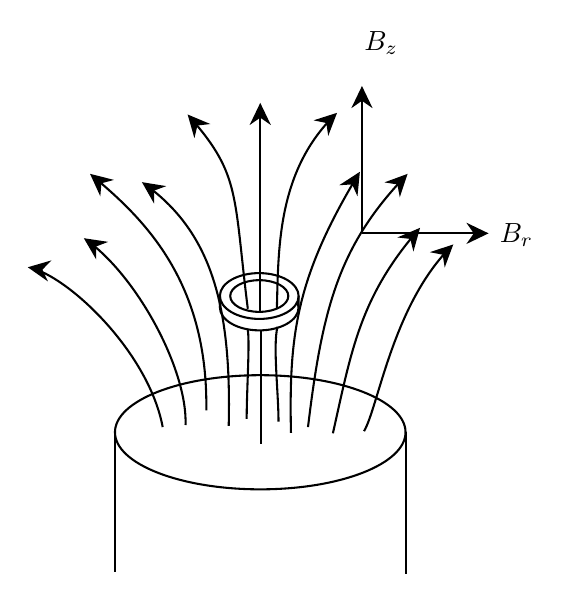
\begin{tikzpicture}[x=0.75pt,y=0.75pt,yscale=-1,xscale=1]
%uncomment if require: \path (0,427); %set diagram left start at 0, and has height of 427

%Shape: Ellipse [id:dp0729966806762341] 
\draw   (272,242.5) .. controls (272,227.31) and (303.34,215) .. (342,215) .. controls (380.66,215) and (412,227.31) .. (412,242.5) .. controls (412,257.69) and (380.66,270) .. (342,270) .. controls (303.34,270) and (272,257.69) .. (272,242.5) -- cycle ;
%Straight Lines [id:da7635427744590266] 
\draw    (272,242.5) -- (272,310) ;
%Straight Lines [id:da4446999648610743] 
\draw    (412,242.5) -- (412,311) ;
%Shape: Ellipse [id:dp8171924606462331] 

\draw [fill={rgb, 245:red, 245; green, 245; blue, 245 }  ,fill opacity=1 ] (322.54,182.3) .. controls (322.57,176.2) and (331.08,171.3) .. (341.55,171.34) .. controls (352.02,171.38) and (360.5,176.35) .. (360.47,182.44) .. controls (360.45,188.54) and (351.94,193.45) .. (341.47,193.41) .. controls (330.99,193.37) and (322.52,188.39) .. (322.54,182.3) -- cycle ;
%Shape: Ellipse [id:dp9639894676210845] 

\draw  [fill={rgb, 245:red, 245; green, 245; blue, 245 }  ,fill opacity=1 ] (322.56,176.78) .. controls (322.59,170.69) and (331.1,165.78) .. (341.57,165.82) .. controls (352.05,165.86) and (360.52,170.83) .. (360.49,176.93) .. controls (360.47,183.02) and (351.96,187.93) .. (341.49,187.89) .. controls (331.01,187.85) and (322.54,182.88) .. (322.56,176.78) -- cycle ;
%Straight Lines [id:da06528213215234935] 

\draw  [fill={rgb, 245:red, 245; green, 245; blue, 245 }  ,fill opacity=1 ]  (322.57,175.95) -- (322.54,182.3) ;
%Straight Lines [id:da37539512217291704] 
\draw [fill={rgb, 245:red, 245; green, 245; blue, 245 }  ,fill opacity=1 ]   (360.49,176.93) -- (360.47,182.44) ;
%Shape: Ellipse [id:dp7858923345915254] 
\draw   (327.53,176.85) .. controls (327.53,172.64) and (333.8,169.22) .. (341.53,169.22) .. controls (349.26,169.22) and (355.52,172.64) .. (355.52,176.85) .. controls (355.52,181.07) and (349.26,184.49) .. (341.53,184.49) .. controls (333.8,184.49) and (327.53,181.07) .. (327.53,176.85) -- cycle ;

%Straight Lines [id:da338498725340286] 
\draw    (342,184) -- (342,86.8) ;
\draw [shift={(342,83.8)}, rotate = 450] [fill={rgb, 255:red, 0; green, 0; blue, 0 }  ][line width=0.08]  [draw opacity=0] (10.72,-5.15) -- (0,0) -- (10.72,5.15) -- (7.12,0) -- cycle    ;
%Curve Lines [id:da9895800220233595] 
\draw    (350,183) .. controls (350.78,154.92) and (350.04,117.9) .. (376.88,90.67) ;
\draw [shift={(379,88.6)}, rotate = 496.62] [fill={rgb, 255:red, 0; green, 0; blue, 0 }  ][line width=0.08]  [draw opacity=0] (10.72,-5.15) -- (0,0) -- (10.72,5.15) -- (7.12,0) -- cycle    ;
%Curve Lines [id:da7767319688985757] 
\draw    (356.8,242.8) .. controls (355.82,196.5) and (358.9,168.84) .. (388.62,119.28) ;
\draw [shift={(390,117)}, rotate = 481.29] [fill={rgb, 255:red, 0; green, 0; blue, 0 }  ][line width=0.08]  [draw opacity=0] (10.72,-5.15) -- (0,0) -- (10.72,5.15) -- (7.12,0) -- cycle    ;
%Curve Lines [id:da4645859456621029] 
\draw    (336,183) .. controls (329.18,128.4) and (332.43,118.67) .. (308.87,91.52) ;
\draw [shift={(307,89.4)}, rotate = 408.37] [fill={rgb, 255:red, 0; green, 0; blue, 0 }  ][line width=0.08]  [draw opacity=0] (10.72,-5.15) -- (0,0) -- (10.72,5.15) -- (7.12,0) -- cycle    ;
%Curve Lines [id:da7043644420679889] 
\draw    (326.8,239.4) .. controls (328.17,181.68) and (318.5,146.77) .. (287.43,123.75) ;
\draw [shift={(285,122)}, rotate = 394.88] [fill={rgb, 255:red, 0; green, 0; blue, 0 }  ][line width=0.08]  [draw opacity=0] (10.72,-5.15) -- (0,0) -- (10.72,5.15) -- (7.12,0) -- cycle    ;
%Straight Lines [id:da3904860160209753] 
\draw    (342.46,193.41) -- (342.46,248) ;
%Curve Lines [id:da839563482499617] 
\draw    (336,193) .. controls (337,200) and (335.46,222) .. (335.46,236) ;
%Curve Lines [id:da9291187636763794] 
\draw    (350.33,191.67) .. controls (348,200.33) and (350.79,223.34) .. (350.79,237.34) ;
%Curve Lines [id:da32485425315181105] 
\draw    (365,240) .. controls (371.86,183.16) and (379.68,153.21) .. (411.05,120.04) ;
\draw [shift={(413,118)}, rotate = 494.14] [fill={rgb, 255:red, 0; green, 0; blue, 0 }  ][line width=0.08]  [draw opacity=0] (10.72,-5.15) -- (0,0) -- (10.72,5.15) -- (7.12,0) -- cycle    ;
%Curve Lines [id:da34465617714496455] 
\draw    (316,232) .. controls (316.97,169.92) and (285.95,139.83) .. (262.18,119.83) ;
\draw [shift={(260,118)}, rotate = 399.81] [fill={rgb, 255:red, 0; green, 0; blue, 0 }  ][line width=0.08]  [draw opacity=0] (10.72,-5.15) -- (0,0) -- (10.72,5.15) -- (7.12,0) -- cycle    ;
%Curve Lines [id:da5363857316680103] 
\draw    (377,243) .. controls (385.82,203.8) and (389.84,178.05) .. (417.29,145.97) ;
\draw [shift={(419,144)}, rotate = 491.31] [fill={rgb, 255:red, 0; green, 0; blue, 0 }  ][line width=0.08]  [draw opacity=0] (10.72,-5.15) -- (0,0) -- (10.72,5.15) -- (7.12,0) -- cycle    ;
%Curve Lines [id:da9124063595562211] 
\draw    (306,239) .. controls (306.97,212.81) and (283.48,168.74) .. (259.25,150.61) ;
\draw [shift={(257,149)}, rotate = 394.22] [fill={rgb, 255:red, 0; green, 0; blue, 0 }  ][line width=0.08]  [draw opacity=0] (10.72,-5.15) -- (0,0) -- (10.72,5.15) -- (7.12,0) -- cycle    ;
%Curve Lines [id:da11116789361747137] 
\draw    (392,242) .. controls (398.86,230.24) and (405.72,181.98) .. (433.29,153.71) ;
\draw [shift={(435,152)}, rotate = 496.01] [fill={rgb, 255:red, 0; green, 0; blue, 0 }  ][line width=0.08]  [draw opacity=0] (10.72,-5.15) -- (0,0) -- (10.72,5.15) -- (7.12,0) -- cycle    ;
%Curve Lines [id:da35480073219801134] 
\draw    (295,240) .. controls (288.35,204.85) and (251.92,169.7) .. (232.86,163.7) ;
\draw [shift={(230,163)}, rotate = 369.46000000000004] [fill={rgb, 255:red, 0; green, 0; blue, 0 }  ][line width=0.08]  [draw opacity=0] (10.72,-5.15) -- (0,0) -- (10.72,5.15) -- (7.12,0) -- cycle    ;
%Straight Lines [id:da18894934454124246] 
\draw    (391,146.67) -- (449,146.67) ;
\draw [shift={(452,146.67)}, rotate = 180] [fill={rgb, 255:red, 0; green, 0; blue, 0 }  ][line width=0.08]  [draw opacity=0] (10.72,-5.15) -- (0,0) -- (10.72,5.15) -- (7.12,0) -- cycle    ;
%Straight Lines [id:da36750597190613] 
\draw    (391,146.67) -- (391,78.67) ;
\draw [shift={(391,75.67)}, rotate = 450] [fill={rgb, 255:red, 0; green, 0; blue, 0 }  ][line width=0.08]  [draw opacity=0] (10.72,-5.15) -- (0,0) -- (10.72,5.15) -- (7.12,0) -- cycle    ;

% Text Node
\draw (456,140.4) node [anchor=north west][inner sep=0.75pt]    {$B_{r}$};
% Text Node
\draw (390.67,48.07) node [anchor=north west][inner sep=0.75pt]    {$B_{z}$};


\end{tikzpicture}

\end{center}
Ban đầu, cường độ dòng điện trong nhẫn bằng $0$. Khi người ta buông nhẫn ra, nó bắt đầu chuyển động xuống dưới theo phương thẳng đứng. Từ những dữ liệu dưới đây, hãy xác định cách nhẫn dịch chuyển sau đó và cường độ dòng điện chạy trong nhẫn?\\
Dữ liệu:\\
Thông số của nhẫn như sau, khối lượng $ m=50\ \mathrm{mg}$, bán kính $r_0=0,5\ \mathrm{cm}$, độ tự cảm $ L=1,3\times{10^{-8}}\ \mathrm{H}$.\\
Tọa độ ban đầu của tâm vòng			$ z=0$, $ r=0$.\\
Các hằng số:						$B_0=0,01\ \mathrm{T}$, $\alpha=2\ \mathrm{m^{-1}}$, $\beta=32\ \mathrm{m^{-1}}$.
\end{vd}
\begin{loigiai}
Từ thông tổng hợp tại vị trí của nhẫn được tạo thành bởi từ trường bên ngoài và do hiện tượng tự cảm,
$$\Phi=B_z\pi r_0^2+LI.$$
Bất kì sự thay đổi nào trong từ thông đều gây ra dòng điện:
$$ RI=\dfrac{\Delta\Phi}{\Delta t}.$$
Tuy nhiên, cường độ dòng điện phải bằng $0$ vì điện trở của nhẫn siêu dẫn là bằng $0$. Do đó, từ thông qua nhẫn không đổi, tức là
$$\Phi=B_0\left(1-\alpha z\right)\pi r_0^2+LI=const.$$
Dựa vào điều kiện đầu $(z=0, I=0)$, ta tìm được giá trị không đổi đó là $$\Phi=B_0\pi r_0^2.$$
Cường độ dòng điện trong nhẫn có thể xác định được dựa vào các phương trình trên, và ta được
$$ I=\dfrac{1}{L}{B_0}\alpha\pi r_0^2z.$$
Lực Lorentz tác dụng lên nhẫn (chỉ theo phương thẳng đứng do tính đối xứng) là
\begin{equation*}
\begin{aligned}
F_z&=-B_r 2\pi{r_0}I(z)\\&=-\dfrac{2\alpha\beta\pi^2{r_0}^4{B_0}^2}{L}z
\\&=-kz.
\end{aligned}
\end{equation*}
Do đó, lực Lorentz tỉ lệ thuận với tọa độ $z$ của nhẫn, với hệ số tỉ lệ có thể tính được từ các dữ liệu đã cho (Kết quả này chỉ có giá trị với các sự dịch chuyển nhỏ, vì cảm ứng từ không được mô tả đầy đủ bằng các công thức đã cho đối với sự dịch chuyển lớn).\\
Phương trình chuyển động của nhẫn
$$ m{a_z}=F_z-mg=-kz-mg.$$
Có nghĩa là nhẫn dao động điều hòa xung quanh vị trí cân bằng $z_0=-\dfrac{mg}{k}$ với
$ z(t)-z_0=A\cos\omega t$,
trong đó $\omega=\sqrt{\dfrac{k}{m}}$. Từ điều kiện ban đầu, $ A=-z_{0}$, và do đó
$$ z(t)=\dfrac{g}{\omega^2}\left(\cos\omega t-1\right).$$
Tọa độ $z$ không bao giờ dương, và do đó lực Lorentz luôn hướng lên trên, bằng $0$ tại vị trí cao nhất của dao động. Dòng điện luôn chảy cùng chiều xung quanh nhẫn.\\
Thay thế dữ liệu số cho $\omega=31,2\ \mathrm{s^{-1}}$ và $ A=1\ \mathrm{cm}$. Sự phụ thuộc của cường độ dòng điện theo thời gian là
$$ I=\dfrac{1}{L}{B_0}\alpha\pi r_0^2z(t)=\dfrac{1}{L}{B_0}\alpha\pi r_0^2A\left(\mathrm{cos}\omega t-1\right).$$
Cường độ dòng điện cực đại là $I_{\max}=39\mathrm{A}$.
\end{loigiai}



 \begin{vd}[Nêm từ trường]
%OPhO open round 2021
     Một vật nhỏ khối lượng $m$ và điện tích $Q$ được đặt trên một mặt phẳng nghiêng với góc nghiêng $\alpha=40^\circ$. Hệ số ma sát giữa vật với mặt phẳng là $\mu=0,3$. Hệ đặt trong một từ trường đều với cảm ứng từ $B_0$ có phương vuông góc với mặt phẳng. Vận tốc vật khi ổn định được tính theo công thức $v=\beta\dfrac{mg}{QB_0}$. Xác định $\beta$. Không bỏ qua ảnh hưởng của trọng lực.
    \begin{center}
        
\includegraphics[width=\textwidth]{Anh/04.pdf}
    \end{center}
\end{vd}
 \begin{loigiai}
        Giả sử khi ổn định vận tốc của vật như hình vẽ. Lúc đó các lực tác dụng lên vật cân bằng với nhau.\\
        \begin{minipage}{0.5\textwidth}
         Ta có 
        \begin{equation*}
            \begin{aligned}
             &F_t^2+F_{ms}^2=P_t^2\\
             \Leftrightarrow&\left(mvB \right) ^2+\left(\mu mg\cos\alpha\right)^2=\left(mg\sin\alpha\right)^2\\
             \Leftrightarrow& v=\frac{mg}{QB}\sqrt{\sin^2\alpha-\cos^2\alpha\mu^2}.
            \end{aligned}
        \end{equation*}
        \end{minipage}
       \begin{minipage}{0.5\textwidth}
        \begin{center}
\tikzset{every picture/.style={line width=0.75pt}} %set default line width to 0.75pt        

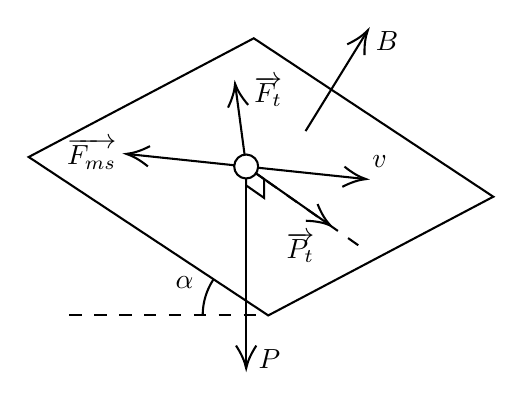
\begin{tikzpicture}[x=0.75pt,y=0.75pt,yscale=-1,xscale=1]
%uncomment if require: \path (0,197); %set diagram left start at 0, and has height of 197

%Shape: Parallelogram [id:dp22006773776345456] 
\draw  [fill={rgb, 255:red, 0; green, 0; blue, 0 }  ,fill opacity=0 ] (347.04,13) -- (238.61,70.2) -- (354.02,146.53) -- (462.45,89.33) -- cycle ;
%Straight Lines [id:da7592591969205111] 
\draw  [dash pattern={on 4.5pt off 4.5pt}]  (258.16,146.53) -- (354.02,146.53) ;
%Straight Lines [id:da4614904307771164] 
\draw    (343.38,74.78) -- (382.3,102.02) ;
\draw [shift={(383.93,103.17)}, rotate = 215] [color={rgb, 255:red, 0; green, 0; blue, 0 }  ][line width=0.75]    (10.93,-4.9) .. controls (6.95,-2.3) and (3.31,-0.67) .. (0,0) .. controls (3.31,0.67) and (6.95,2.3) .. (10.93,4.9)   ;
%Straight Lines [id:da6610837876111635] 
\draw    (287.65,68.92) -- (399.11,80.63) ;
\draw [shift={(401.1,80.84)}, rotate = 186] [color={rgb, 255:red, 0; green, 0; blue, 0 }  ][line width=0.75]    (10.93,-4.9) .. controls (6.95,-2.3) and (3.31,-0.67) .. (0,0) .. controls (3.31,0.67) and (6.95,2.3) .. (10.93,4.9)   ;
\draw [shift={(285.66,68.71)}, rotate = 6] [color={rgb, 255:red, 0; green, 0; blue, 0 }  ][line width=0.75]    (10.93,-4.9) .. controls (6.95,-2.3) and (3.31,-0.67) .. (0,0) .. controls (3.31,0.67) and (6.95,2.3) .. (10.93,4.9)   ;
%Straight Lines [id:da9236762930555706] 
\draw    (343.38,74.78) -- (338.31,36.9) ;
\draw [shift={(338.04,34.92)}, rotate = 442.38] [color={rgb, 255:red, 0; green, 0; blue, 0 }  ][line width=0.75]    (10.93,-4.9) .. controls (6.95,-2.3) and (3.31,-0.67) .. (0,0) .. controls (3.31,0.67) and (6.95,2.3) .. (10.93,4.9)   ;
%Straight Lines [id:da5753895087853571] 
\draw  [dash pattern={on 4.5pt off 4.5pt}]  (343.38,74.78) -- (400.79,115.11) ;
%Straight Lines [id:da2045020518362104] 
\draw    (343.38,74.78) -- (343.38,169.98) ;
\draw [shift={(343.38,171.98)}, rotate = 270] [color={rgb, 255:red, 0; green, 0; blue, 0 }  ][line width=0.75]    (10.93,-4.9) .. controls (6.95,-2.3) and (3.31,-0.67) .. (0,0) .. controls (3.31,0.67) and (6.95,2.3) .. (10.93,4.9)   ;
%Shape: Arc [id:dp7990414879661973] 
\draw  [draw opacity=0] (322.42,146.39) .. controls (322.45,140.05) and (324.35,134.15) .. (327.59,129.21) -- (354.02,146.53) -- cycle ; \draw   (322.42,146.39) .. controls (322.45,140.05) and (324.35,134.15) .. (327.59,129.21) ;
%Shape: Parallelogram [id:dp14877094118660716] 
\draw  [fill={rgb, 255:red, 0; green, 0; blue, 0 }  ,fill opacity=0 ] (352.04,80.82) -- (352.04,89.93) -- (343.38,83.89) -- (343.38,74.78) -- cycle ;
%Shape: Ellipse [id:dp9129783011120693] 
\draw  [fill={rgb, 255:red, 255; green, 255; blue, 255 }  ,fill opacity=1 ] (338.12,72.39) .. controls (339.43,69.49) and (342.86,68.2) .. (345.76,69.52) .. controls (348.67,70.83) and (349.95,74.25) .. (348.64,77.16) .. controls (347.32,80.06) and (343.9,81.35) .. (341,80.04) .. controls (338.09,78.72) and (336.8,75.3) .. (338.12,72.39) -- cycle ;
%Straight Lines [id:da7096050059389993] 
\draw    (372,57.7) -- (400.91,10.89) ;
\draw [shift={(401.96,9.19)}, rotate = 481.7] [color={rgb, 255:red, 0; green, 0; blue, 0 }  ][line width=0.75]    (10.93,-4.9) .. controls (6.95,-2.3) and (3.31,-0.67) .. (0,0) .. controls (3.31,0.67) and (6.95,2.3) .. (10.93,4.9)   ;

% Text Node
\draw (402.63,68.14) node [anchor=north west][inner sep=0.75pt]    {$\ot{v}$};
% Text Node
\draw (347.86,161.63) node [anchor=north west][inner sep=0.75pt]    {$\ot{P}$};
% Text Node
\draw (361.36,104.79) node [anchor=north west][inner sep=0.75pt]    {$\overrightarrow{P_{t}}$};
% Text Node
\draw (345.86,29.66) node [anchor=north west][inner sep=0.75pt]    {$\overrightarrow{F_{t}}$};
% Text Node
\draw (255.58,59.85) node [anchor=north west][inner sep=0.75pt]    {$\overrightarrow{F_{ms}}$};
% Text Node
\draw (307.84,126.37) node [anchor=north west][inner sep=0.75pt]    {$\alpha $};
% Text Node
\draw (404.4,8.39) node [anchor=north west][inner sep=0.75pt]    {$\ot{B}$};
\end{tikzpicture}
        \end{center}
       \end{minipage}
    Từ đó suy ra $$\beta=\sqrt{\sin^2\alpha-\cos^2\alpha\mu^2} \approx 0.6.$$
    \end{loigiai}
    
    \begin{vd}[Sự va chạm của tấm dẫn điện]
    Một tấm phẳng mỏng hình vuông với cạnh dài $s=5\dv{cm}$, điện tích ban đầu $q=0.1\dv{\mu C}$, và khối lượng $m=100\dv{g}$ được kích thích và chuyển động giữa hai mặt phẳng vô hạn dẫn điện cách nhau một khoảng $d=0.5\dv{cm}\ll s$ và được tích điện trái dấu nhau $\pm \sigma=\pm50\dv{\mu C/m^2}$. Sau một khoảng thời gian dài thì tấm phẳng ở chính giửa hai mặt và có vận tốc $v=3\dv{m/s}$ và hợp với phương ngang một góc $\theta=30^\circ$. Hỏi sẽ có bao nhiêu va chạm xảy ra khi tấm di chuyển được một đoạn $L=15\dv{m}$ theo phương ngang. Coi mọi va chạm là đàn hồi, bỏ qua hiện tượng hưởng ứng và ảnh hưởng của trọng lực.
    \begin{center}
         
\includegraphics[width=\textwidth]{Anh/13.pdf}
    \end{center}
\end{vd}
\begin{loigiai}
Sau khi va chạm với mặt phẳng $+\sigma$ thì tấm sẽ trao đổi điện tích với mặt phẳng. Điện tích của tấm lúc này là $\sigma s^2$. Tương tự khi tấm va chạm với mặt phẳng $-\sigma$, tấm sẽ trao đổi điện tích và có điện tích là $-\sigma s^2$. Trong quá trình chuyển động, độ lớn gia tốc của tấm là không đổi $$a=\frac{\sigma^2s^2}{\varepsilon_0m}\approx7.06\dv{m/s^2}.$$
Các va chạm là hoàn toàn đàn hồi.
Ta có $$L=v\cos(\theta)t\Leftrightarrow t=\frac{L}{v\cos(\theta)}.$$
Tổng quãng đường đi được theo phương thẳng đứng
\begin{equation*}
    \begin{aligned}
     D&=v\sin(\theta)t+\frac{a}{2}t^2\\
     &=\tan(\theta)L+\frac{aL^2}{2v^2\cos^2(\theta)}.
    \end{aligned}
\end{equation*}
Số lần tấm va chạm với mặt phẳng
$$n=\left \lfloor{\frac{D+\dfrac{d}{2}}{d}}\right \rfloor=25273.$$
Với $\left \lfloor{x}\right \rfloor$ là số nguyên lớn nhất không vượt quá $x$.
\end{loigiai}

    \begin{vd}[Kéo thẳng đường cong]
    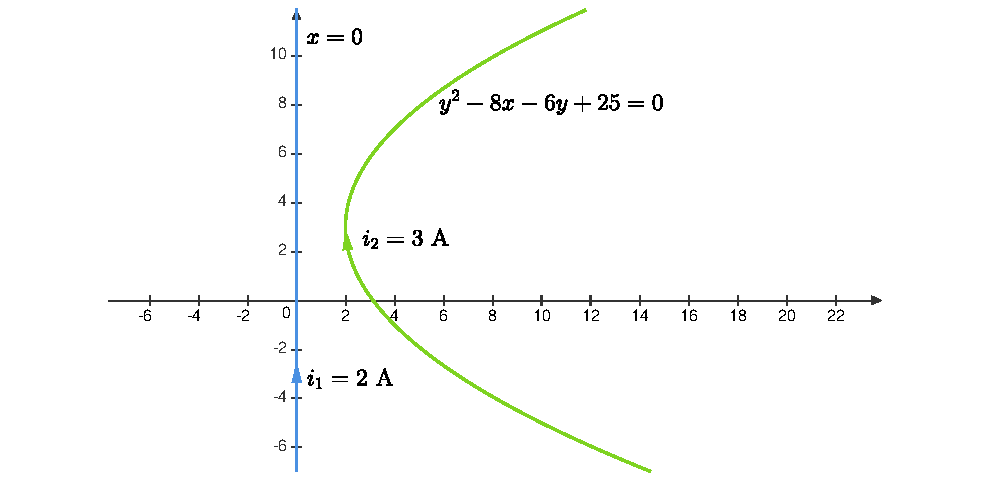
\includegraphics[width=\textwidth]{Anh/c1.pdf}\\
    Hai dây dẫn vô hạn có dòng điện không đổi chạy qua là $i_1=2\dv{A}$ và $i_2=3\dv{A}$ như trên hình vẽ. Phương trình miêu tả hình dạng hai dây lần lượt là $x=0$ và $y^2-8x-6y+25=0$, với $x$ và $y$ tính theo đơn vị $\mathrm{m}$. Tìm lực do dây này tác dụng lên dây kia.
    \end{vd}
    \begin{loigiai}
    Từ trường tạo ra bởi dây dẫn 1 tại một điểm nằm trong mặt phẳng $Oxy$
    $$B(x)=-\dfrac{\mu_0i_1}{2\pi x}.$$
    Thành phần theo phương $Ox$ lực từ tác dụng lên một phần tử của dây 2:
    \[\begin{aligned}
             \dd F_x&=B(x)i_2\dd y\\
             &=-\dfrac{\mu_0i_1i_2}{2\pi x}\dd y.
        \end{aligned}\tag{1} \label{c111}\]
    Lại có 
    \[ y^2-8x-6y+25=0\Leftrightarrow x=\dfrac{y^2-6y+25}{8} \tag{2} \label{c112}.\]
    Từ (\ref{c111}) và (\ref{c112}) ta có
    \begin{equation*}
             F_x=\tiph{-\infty}{\infty}{-\dfrac{4\mu_0i_1i_2}{\pi\tron{y^2-6y+25}}}{y}.
    \end{equation*}
    Đặt $u=y-3$, ta có
    \begin{equation*}
             F_x=\tiph{-\infty}{\infty}{-\dfrac{4\mu_0i_1i_2}{\pi\tron{u^2+16}}}{u}.
    \end{equation*}
    Đặt $\dfrac{u}{4}=\tan\alpha$, ta có
    \begin{equation*}
        \begin{aligned}
             F_x&=\tiph{-\frac{\pi}{2}}{\frac{\pi}{2}}{-\dfrac{\mu_0i_1i_2}{4\pi\tron{\tan^2\alpha+1}}\dfrac{4}{\cos^2\alpha}}{\alpha}\\
             &=\tiph{-\frac{\pi}{2}}{\frac{\pi}{2}}{-\dfrac{\mu_0i_1i_2}{\pi}}{\alpha}\\
             &=-\mu_0i_1i_2.
        \end{aligned}
    \end{equation*}
    Vậy hai dây hút nhau với một lực bằng $7.54\times10^{-6}\dv{N}$.
    \end{loigiai}
    
\begin{vd}[Magnetars]
Từ trường xuất hiện ở tất cả mọi nơi xung quanh chúng ta. Một vài giá trị của từ trường điển hình: từ trường Trái Đất: $25-60~\mathrm{\mu T}$; vệt đen ở Mặt Trời: $0,3~\mathrm{T}$; nam châm vĩnh cữu mạnh: khoảng $1~\mathrm{T}$; từ trường được duy trì liên tục trong phòng thí nghiệm: lên đến $45~\mathrm{T}$; neutron starts và magnetars: lên đến $10^{11}~\mathrm{T}$. Sau đây, chúng ta sẽ nghiên cứu một vài tính chất của từ trường mạnh.\\
Mật độ năng lượng từ trường là $\omega=B^2\dfrac{1}{2\mu \mu_0}$, với $\mu_0\approx1,3\times 10^{-6}~\mathrm{N/A^2}$ là hằng số từ (hay còn gọi là độ từ thẩm của chân không), và $\mu$ - độ từ thẩm tương đối của môi trường. Hệ đang cố gắng chuyển sang trạng thái năng lượng thấp hơn và do đó vật liệu sắt từ với $\mu \gg 1$ thì bị hút về phía có từ trường mạnh, và các vật liệu nghịch từ với $\mu < 1$ thì bị đẩy ra ngoài. Với các vật liệu nghịch từ, độ cảm từ $\chi=\mu -1$ có giá trị nhỏ, $\chi \ll 1$, và do đó nếu từ trường không đủ lớn thì chỉ gây ra một sự ảnh hưởng nhỏ. Nước là vật liệu nghịch từ với $\chi=-9\times10^{-6}$ và bình thường thì nước chiếm hầu hết trọng lượng của cơ thể động vật, hay nói cách khác, động vật hầu như được tạo nên bởi nước. Do đó, ếch có thể bay lên bên trong từ trường nếu như từ trường đủ mạnh, chúng ta có thể xem hình sau.
\begin{center}
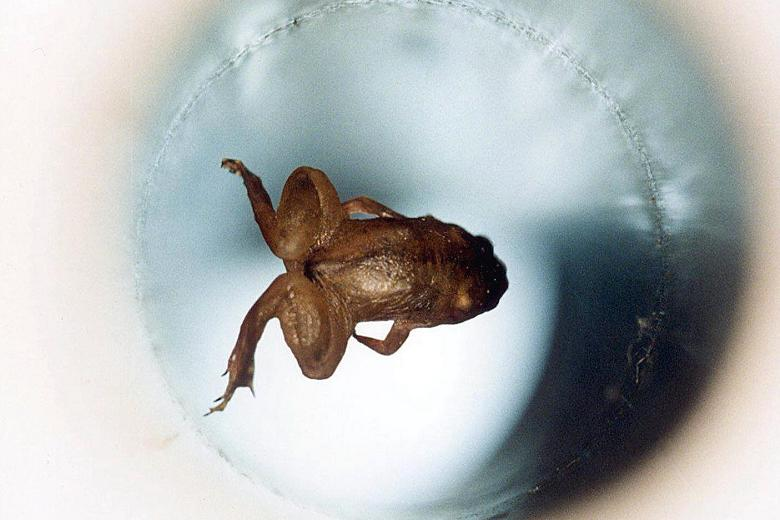
\includegraphics[scale=0.4]{Anh/2016.3.1.jpg}
\end{center}
\begin{enumerate}[1)]
    \item Cho chiều cao của con ếch là $h_{f}$ không quá $h_0=10~\mathrm{mm}$, và chúng ta đơn giản hóa rằng bình phương của cảm ứng từ phụ thuộc tuyến tính vào độ cao $z$ như hình dưới. 
    \begin{center}
        \tikzset{every picture/.style={line width=0.75pt}} %set default line width to 0.75pt        

\begin{tikzpicture}[x=0.75pt,y=0.75pt,yscale=-1,xscale=1]
%uncomment if require: \path (0,300); %set diagram left start at 0, and has height of 300

%Straight Lines [id:da7268528150747415] 
\draw    (212,200.33) -- (411,200.33) ;
\draw [shift={(414,200.33)}, rotate = 180] [fill={rgb, 255:red, 0; green, 0; blue, 0 }  ][line width=0.08]  [draw opacity=0] (10.72,-5.15) -- (0,0) -- (10.72,5.15) -- (7.12,0) -- cycle    ;
%Straight Lines [id:da9151910129710128] 
\draw    (260,247.67) -- (260,95.33) ;
\draw [shift={(260,92.33)}, rotate = 450] [fill={rgb, 255:red, 0; green, 0; blue, 0 }  ][line width=0.08]  [draw opacity=0] (10.72,-5.15) -- (0,0) -- (10.72,5.15) -- (7.12,0) -- cycle    ;
%Straight Lines [id:da478705783765105] 
\draw [color={rgb, 255:red, 230; green, 29; blue, 29 }  ,draw opacity=1 ]   (239,120) -- (260,120) -- (340.33,200.33) -- (354,200.33) ;

% Text Node
\draw (266,87.4) node [anchor=north west][inner sep=0.75pt]    {$B^{2}$};
% Text Node
\draw (217,110.4) node [anchor=north west][inner sep=0.75pt]    {$B_{0}^{2}$};
% Text Node
\draw (247,202.4) node [anchor=north west][inner sep=0.75pt]    {$0$};
% Text Node
\draw (200,192.4) node [anchor=north west][inner sep=0.75pt]    {$0$};
% Text Node
\draw (391,179.4) node [anchor=north west][inner sep=0.75pt]    {$z$};
% Text Node
\draw (333,203.4) node [anchor=north west][inner sep=0.75pt]    {$h_{0}$};


\end{tikzpicture}

    \end{center}
    Tìm giá trị của $B_0$ (đơn vị Teslas) cần để duy trì con ếch ở trạng thái lơ lửng trên không. Biết rằng con ếch có cấu tạo hoàn toàn từ nước (mật độ $\rho=1000~\mathrm{kg/m^3}$); gia tốc rơi tự do là $g=9,8~\mathrm{m/s^2}$. \textit{Gợi ý}: với $\left|\chi\right|\ll1$, chúng ta có thể làm gần đúng $\omega\approx B^2\dfrac{1-\chi}{2\mu_0}$; do đó, biểu thức liên hệ giữa mật độ năng lượng và sự có mặt của nước là $\Delta \omega=B^2\dfrac{1-\chi}{2\mu_0}-B^2\dfrac{1}{2\mu_0}=-B^2\dfrac{\chi}{2\mu_0}$.\\
    Các ngôi sao được cấu tạo từ plasma$-$một chất dẫn điện tốt. Chính vì thế, các đường sức từ sẽ như thể bị "đóng băng" đối với plasma chuyển động (điều này tuần theo định luật cảm ứng Faraday và định luật Kirchoff: do không có điện trở, độ giảm điện áp giữa các vành gần nhau ở bên trong plasma mà ta giả sử gần như bằng không, do đó từ thông không đổi). Nếu một ngôi sao biến thành một ngôi sao neutron, hiệu ứng này sẽ dẫn tới sự tăng tức thời của từ trường, quan sát bản phác thảo các đường sức từ trong trường hợp trước và sau sự biến đổi (nhớ rằng cường độ từ trường tỉ lệ thuận mật độ đường sức từ).
    \begin{center}
        \tikzset{every picture/.style={line width=0.75pt}} %set default line width to 0.75pt        

\begin{tikzpicture}[x=0.75pt,y=0.75pt,yscale=-1,xscale=1]
%uncomment if require: \path (0,300); %set diagram left start at 0, and has height of 300

%Shape: Circle [id:dp6549836949350023] 
\draw  [fill={rgb, 255:red, 248; green, 231; blue, 28 }  ,fill opacity=1 ] (191.12,176.82) .. controls (165.89,155.62) and (162.62,117.98) .. (183.82,92.76) .. controls (205.02,67.53) and (242.66,64.26) .. (267.89,85.46) .. controls (293.12,106.66) and (296.38,144.3) .. (275.18,169.52) .. controls (253.99,194.75) and (216.35,198.02) .. (191.12,176.82) -- cycle ;
%Straight Lines [id:da2858934451028303] 
\draw    (314.72,30.77) -- (149.39,227.52) ;
%Curve Lines [id:da3454539603886295] 
\draw    (186,236.33) .. controls (196,173.33) and (279,71.33) .. (349,63.33) ;
%Curve Lines [id:da20367008645727047] 
\draw    (208,234.33) .. controls (212,182.33) and (276,87.33) .. (362,85.33) ;
%Curve Lines [id:da31253548461166103] 
\draw    (230,230.33) .. controls (219,183.33) and (280,118.33) .. (325,111.33) ;
%Curve Lines [id:da6954594469756084] 
\draw    (121.4,187.11) .. controls (147,181.33) and (192.35,158.13) .. (220,130.33) .. controls (247.65,102.53) and (258,71.33) .. (263.57,17.91) ;
%Curve Lines [id:da7055460410915435] 
\draw    (128,167.33) .. controls (189,138.67) and (240,123.67) .. (245.8,25.51) ;
%Curve Lines [id:da9412388070670608] 
\draw    (135,141.33) .. controls (177,139.33) and (234.43,95.22) .. (223.78,37.95) ;
%Shape: Ellipse [id:dp6904993388159524] 
\draw  [fill={rgb, 255:red, 248; green, 231; blue, 28 }  ,fill opacity=1 ] (312.9,235.74) .. controls (300.78,225.55) and (299.21,207.47) .. (309.39,195.35) .. controls (319.58,183.23) and (337.66,181.66) .. (349.78,191.84) .. controls (361.9,202.03) and (363.47,220.11) .. (353.29,232.23) .. controls (343.1,244.36) and (325.02,245.92) .. (312.9,235.74) -- cycle ;
%Straight Lines [id:da5888993463068299] 
\draw    (372.28,165.56) -- (292.85,260.1) ;
%Curve Lines [id:da7090409488977016] 
\draw    (310.44,264.33) .. controls (315.24,234.06) and (355.12,185.06) .. (388.75,181.21) ;
%Curve Lines [id:da9595209168666552] 
\draw    (321.01,263.37) .. controls (322.93,238.39) and (353.68,192.74) .. (395,191.78) ;
%Curve Lines [id:da6970412667469024] 
\draw    (331.58,261.45) .. controls (326.29,238.87) and (355.6,207.64) .. (377.22,204.27) ;
%Curve Lines [id:da2584482459277204] 
\draw    (279.4,240.68) .. controls (291.7,237.91) and (313.49,226.76) .. (326.77,213.4) .. controls (340.06,200.05) and (345.03,185.06) .. (347.71,159.39) ;
%Curve Lines [id:da6611636099889706] 
\draw    (282.57,231.18) .. controls (314.76,219.65) and (337,206.67) .. (339.17,163.04) ;
%Curve Lines [id:da5617316237885455] 
\draw    (287.05,216.95) .. controls (305.55,221.83) and (333.71,196.53) .. (328.59,169.02) ;

% Text Node
\draw (87,56) node [anchor=north west][inner sep=0.75pt]   [align=left] {Trước khi biến đổi};
% Text Node
\draw (349,244) node [anchor=north west][inner sep=0.75pt]   [align=left] {Sau khi biến đổi};


\end{tikzpicture}

    \end{center}
    \item Biết rằng cảm ứng từ của một ngôi sao là $B_{s}=100~\mathrm{\mu T}$ và mật độ trung bình $\rho_{s}=1400~\mathrm{kg/m^3}$, hãy xác định giá trị của cảm ứng từ $B_{c}$ sau khi ngôi sao ấy biến đổi thành ngôi sao neutron do sự nén của các đường sức từ như đã mô tả ở trên. Mật độ của ngôi sao neutron là $\rho_{n}=5\times10^{17}~\mathrm{kg/m^3}$.
    \item Trên thực tế, từ trường của ngôi sau neutron được tạo ra bằng nhiều cách khác nhau. Bây giờ chúng ta sẽ cùng xem xét một mô hình đã được đơn giản hóa. Phần bên trong của ngôi sao đã biến đổi thành kích thước và mật độ của ngôi sao neutron, nhưng phần bên ngoài vẫn giữ nguyên như cũ. Biết rằng trước khi xảy ra biến đổi, ngôi sao đang xoay như một khối rắn với tốc độ góc $\omega_{s}$. Biểu diễn tốc độ góc mới của phần bên trong ngôi sao $\omega_{n}$ theo $\omega_{s}$, $\rho_{s}$ và $\rho_{n}$.
    \item Tốc độ quay của phần bên ngoài và phần bên trong là khác nhau, do đó các đường sức sẽ bị co giãn, xem hình dưới đây. Để đơn giản hóa: ($a$) chúng ta sử dụng hình học hai chiều, hay nói cách khác là xem những ngôi sao như hình trụ; ($b$) trong khi trường ban đầu là trường lưỡng cực, chúng ta thừa nhận rằng nó là hình trụ đối xứng như đã biểu diễn trong hình vẽ; ($c$) điểm cuối của đường sức thì gắn liền với phần hình trụ bên trong (sao neutron) và lớp vỏ hình trụ bên ngoài (phần còn lại của ngôi sao ban đầu). Cho biết rằng cảm ứng từ tại lớp vỏ ban đầu là $B_0$. Hãy biểu diễn cảm ứng từ $B$ là một hàm theo thời gian $t$ trong vùng mà các đường sức đang bị co giãn với $t \gg 1/ \omega_{n}$ theo $B_0$ và $\omega_{n}$.
    \end{enumerate}
    \begin{center}
        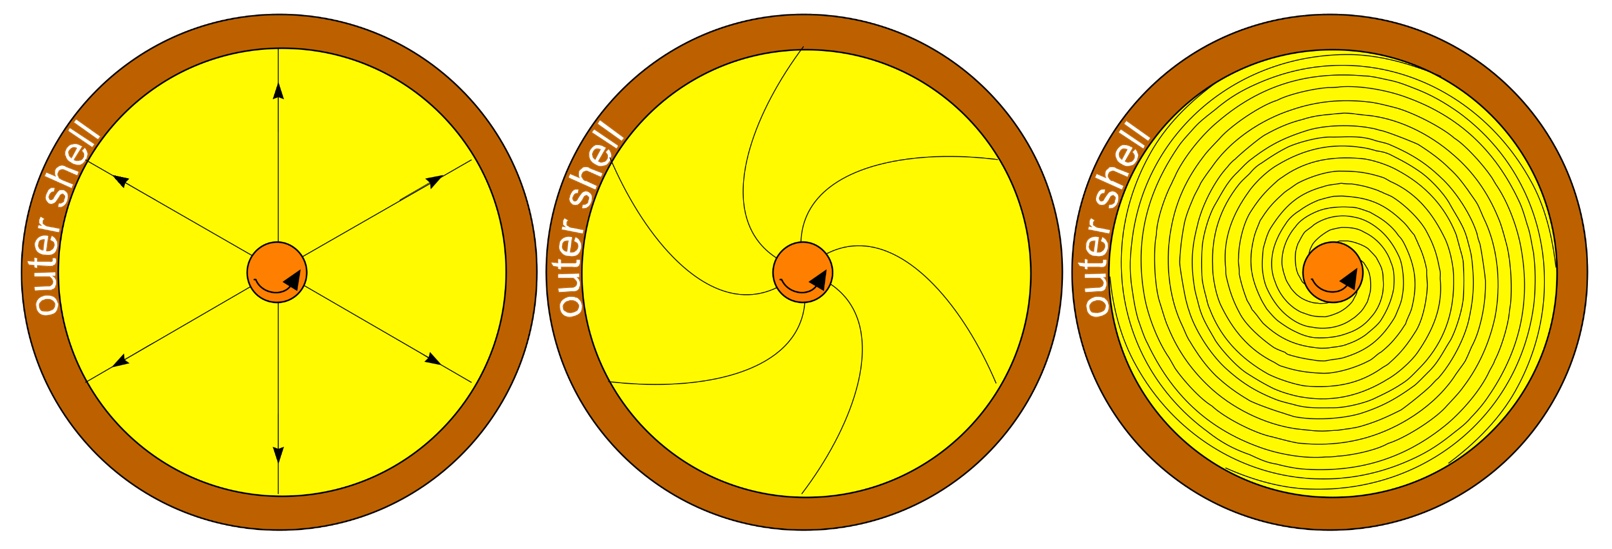
\includegraphics[width= 0.8\textwidth]{Anh/2016.png}
    \end{center}
    \begin{enumerate}[1)]
    \setcounter{enumi}{4}
    \item Do đó, năng lượng được chuyển hóa trong quá trình biến đổi của ngôi sao thì tuân theo: thế năng hấp dẫn đươc chuyển hóa thành động năng (ở đây, chúng ta bỏ qua nhiệt năng) và sau đó là chuyến hóa thành năng lượng từ. Dựa vào đó, hãy tính giá trị cực đại của cảm ứng từ $B_{\max}$ của ngôi sao neutron có khối lượng $M_{n}=4\times10^{30}~\mathrm{kg}$ và bán kính $R_{n}=13~\mathrm{km}$. Nhớ rằng $G=6,67\times10^{-11}~\mathrm{m^3s^{-2}kg^{-1}}$.
    \item Từ trường cực mạnh sẽ có ảnh hưởng đến tính chất hóa học của vật bằng cách thay đổi hình dáng của quỹ đạo electron của vật đó. Điều đó xảy ra khi lực Lorentz tác dụng lên một electron có quỹ đạo trở nên mạnh hơn lực Coulomb do tương tác với hạt nhân nguyên tử. Hãy tính giá trị của cảm ứng từ $B_{H}$ cần thiết để làm biến dạng quỹ đạo của electron của một nguyên tử Hydro có bán kính $R_{H}=5\times10^{-11}~\mathrm{m}$. Chú ý rằng $\dfrac{1}{4\pi\varepsilon_0}=9\times10^9~\mathrm{m/F}$, $e=1,6\times10^{-19}~\mathrm{C}$ và khối lượng của electron $m_{e}=9,1\times10^{-31}~\mathrm{kg}$.
    \item Trong những từ trường cực mạnh, những đám mây electron của nguyên tử có hình dạng như hình trụ. Hãy tính tỉ lệ chiều dài trên đường kính $\kappa=\ell/d$ của những đám mây electron như thế trong những nguyên tử Hydro gần một ngôi sao neutron, trong từ trường $B_{n}=10^8~\mathrm{T}$. Cho biết rằng hằng số Plank $h=6,6\times10^{-34}~\mathrm{J\cdot s}$. \textit{Gợi ý}: bán kính của quỹ đạo cyclotron của một electron trong cơ học lượng tử có thể tính toán bằng cách sử dụng nguyên lí bất định.
\end{enumerate}
\end{vd}
\begin{loigiai}
\begin{enumerate}[1) ]
    \item Nếu chúng ta thay đổi chiều cao của con ếch một lượng $\Delta h$, sự biến thiên trong thế năng sẽ nhỏ hơn sự thay đổi của năng lượng từ trường.\\Chúng ta lưu ý rằng với mỗi điểm của con ếch, sự biến thiên của năng lượng từ trường là như nhau, do đó chúng ta có thể biểu diễn như sau
    \[\Delta E=-V\dfrac{\Delta(B^2)\chi}{2\mu_0}=V\dfrac{B_0^2\chi\Delta h}{2h_0\mu_0}.\]
    Độ biến thiên của thế năng là
    \[\Delta \Pi=V\rho g\Delta h. \]
    Do
    \[
    \begin{cases}
    \Delta E+\Delta \Pi &<0,\\
    V\dfrac{B_0^2\chi\Delta h}{2h_0\mu_0}+V\rho g\Delta h&<0.
    \end{cases}
    \]
    Điều đó có nghĩa:
    \[B_0>\sqrt{-\dfrac{2h_0\mu_0\rho g}{\chi}}.\]
    Thay số ta được:
    \[B_0=5,32~\mathrm{T}.\]
    \item Chúng ta sẽ quan sát một mẩu của ngôi sao có thể tích $V_0$ trước khi biến đổi và là $V_1$ sau khi xảy ra sự biến đổi. Khối lượng trước và sau là không đổi. Điều đó có nghĩa là:
    \[V_0\rho_{s}=V_1\rho_{n}.\]
    Bán kính của ngôi sao tỉ lệ với $V^{\frac{1}{3}}$ và diện tích mặt cắt ngang tỉ lệ với $V^{\frac{2}{3}}$.\\
    Tổng điện trường đi qua thể tích ấy vẫn không đổi trước và sau khi xảy ra sự biến đổi:
    \[B_{s}V_0^{\frac{2}{3}}=B_{n}V_1^{\frac{2}{3}}.\]
    Bây giờ chúng ta có thể biểu diễn $B_{n}$
    \[B_{n}=B_{s}\left(\dfrac{V_0}{V_1}\right)^{\frac{2}{3}}=B_{s}\left(\dfrac{\rho_{n}}{\rho_{s}}\right)^{\frac{2}{3}}.\]
    Thay số
    \[B_{n}=5,0\times10^5~\mathrm{T}.\]
    \item Trong suốt quá trình xảy ra sự biến đổi thì không có sự xuất hiện của momen quay của ngôi sao. Điều đó có nghĩa là moment động lượng vẫn được bảo toàn. Do đó:
    \[\dfrac{2}{5}MR^2_{s}\omega_{s}=\dfrac{2}{5}MR_{n}^2\omega_{n}.\]
    Vì $R_{s}$ tỉ lệ nghịch với $\rho_{s}^\frac{1}{3}$. Chúng ta có $\omega_{n}$ sẽ là
    \[\omega_{n}=\omega_{s}\dfrac{R_{s}^2}{R_{n}^2}=\omega_{s}\left(\dfrac{\rho_{n}}{\rho_{s}}\right)^{\frac{2}{3}}.\]
    \item Sau thời gian $t$, ngôi sao neutron quay được một góc $\beta=\omega_{n}t$.\\
    Từ trường xuyên qua bất kì đường xuyên tâm nào từ tâm của ngôi sao neutron có giá trị trung bình là $N=\dfrac{\beta}{2\pi}=\dfrac{\omega_{n}t}{2\pi}$ lần.\\
    Tổng từ thông đi qua lớp vỏ ngoài vẫn giữ nguyên không đổi  và có giá trị luôn là $\Phi=2\pi R_0B_0$, với $R_0$ là bán kính của lớp vỏ ngoài. Điều đó có nghĩa là từ thông đi qua bất kì đường xuyên tâm nào là $\Phi N$.\\
    Do đó
    \[BR_0=2\pi R_0 B_0N=R_0B_0\omega_{n}t.\]
    Và cuối cùng, ta được
    \[B=B_0\omega_{n}t.\]
    \item Chúng ta có thể tìm thế năng hấp dẫn bằng cách tích phân: chúng ta tưởng tượng rằng khi loại bỏ từng lớp vật liệu dày $\mathrm{d}x$, bắt đầu từ phía ngoài cùng. Thế năng của quả cầu rỗng của vật bên trong có độ dày $\mathrm{d}x$ trong trường trọng lực là
    \[\mathrm{d}\Pi=-G\dfrac{(4\pi x^2\mathrm{d}x\rho_{n})\frac{4}{3}\pi x^3\rho_{n}}{x}=-\dfrac{16\pi^2}{3}G\rho_{n}^2x^4\mathrm{d}x.\]
    Tích phân từ $x=0$ đến $x=R_{n}$, ta được:
    \[\Pi=-\dfrac{16\pi^2}{15}G\rho_n^2 R_{n}^5=-\dfrac{3}{5}\dfrac{GM_{n}^2}{R_{n}}.\]
    Thế năng này chính bằng năng lượng của từ trường
    \[\Pi=\dfrac{4}{3}\pi R^3B_{n}^2\dfrac{1}{2\mu_0}.\]
    Giải tìm $B_{n}$, ta được
    \[B_{n}=3\dfrac{M}{R^2}\sqrt{\dfrac{\mu_0G}{10\pi}}.\]
    Thay số
    \[B_{n}=1,18\times 10^{14}~\mathrm{T}.\]
    \item Quỹ đạo của electron sẽ bị bóp méo khi lực Lorentz dần có độ lớn gần bằng của lực Coulomb.\\
    Độ lớn lực Coulomb là
    \[F_1=\dfrac{1}{4\pi \varepsilon_0}\dfrac{e^2}{R_{H}^2},\]
    Mặt khác
    \[F_1=\dfrac{m_{e}v^2}{R_{H}},\]
    Chúng ta có thể suy ra vận tốc của electron là
    \[v=e\sqrt{\dfrac{1}{4\pi \varepsilon_0 R_{H}m_{e}}}.\]
    Khi đó lực Lorentz sẽ là
    \[F_2\approx evB.\]
    Thế $v$ đã tìm được ở trên, ta được
    \[F_2=e^2B\dfrac{1}{\sqrt{4\pi \varepsilon_0 R_{H}m_{e}}}.\]
    Từ điều kiện $F_1\approx F_2$, ta có giá trị của cảm ứng từ
    \[B=\sqrt{\dfrac{m_{e}}{4\pi \varepsilon_0 R_{H}^3}}.\]
    Thay số ta được
    \[B=2,56\times 10^5~\mathrm{T}.\]
    \item Vuông góc với từ trường, lực Lorentz sẽ lớn hơn lực Coulomb rất nhiều vì từ trường $B_{n}$ lớn hơn rất nhiều so với từ trường được tính ở câu trước. Điều đó có nghĩa là trong mặt phẳng vuông góc, electron chuyển động theo quỹ đạo cyclotron tròn.
    Chúng ta có
    \[\dfrac{m_{e}v^2}{R_1}=evB_{n}, \tag{1} \label{2016.1}\]
    với $R_1 = d/2$ là bán kính của quỹ đạo. Bây giờ chúng ta sử dụng nguyên lí bất định. Sai số của động lượng là
    \[\Delta p=2m_{e}v.\]
    Sai số của tọa độ là
    \[\Delta x=2R_1.\]
    Ta có
    \[4m_{e}vR_1\approx \hbar.\]
    Thay $m_{e}v=\dfrac{\hbar}{4R_1}$ vào (\ref{2016.1}), ta được
    \[\dfrac{\hbar}{R_1^2}=4eB_{n}.\]
    Suy ra
    \[R_1=\sqrt{\dfrac{\hbar}{4eB_{n}}}.\]
    Chiều dài của khối trụ vẫn giữa giá trị không đổi là $R_{H}$ bởi vì lực Lorentz không tác dụng lên electron theo phương đó (song song với từ trường). Do đó ta có tỉ lệ giữa chiều dài và đường kính sẽ xấp xỉ bằng
    \[\kappa=\dfrac{R_{H}}{R_1}=2R_{H}\sqrt{\dfrac{eB_{n}}{\hbar}}.\]
    Thay số ta được
    \[\kappa=39\approx 40.\]
    Chú ý rằng khi chúng ta thực hiện tính toán với magnetars khi $B=1\times10^{11}~\mathrm{T}$, các electron thuộc quỹ đạo sẽ đạt đến gần tốc độ ánh sáng.
\end{enumerate}
\end{loigiai}


\begin{vd}[Hiệu ứng spin $-$ Hall]
Ta biết rằng khi một điện trường và một từ trường tác dụng vuông góc lên một miếng bán dẫn, một điện áp $V_{H}$ vuông góc với phương chuyển động của các điện tích sẽ được tạo ra (xem hình vẽ). Hiện tượng này được gọi là hiệu ứng Hall.


\begin{center}
\tikzset{every picture/.style={line width=0.75pt}} %set default line width to 0.75pt        

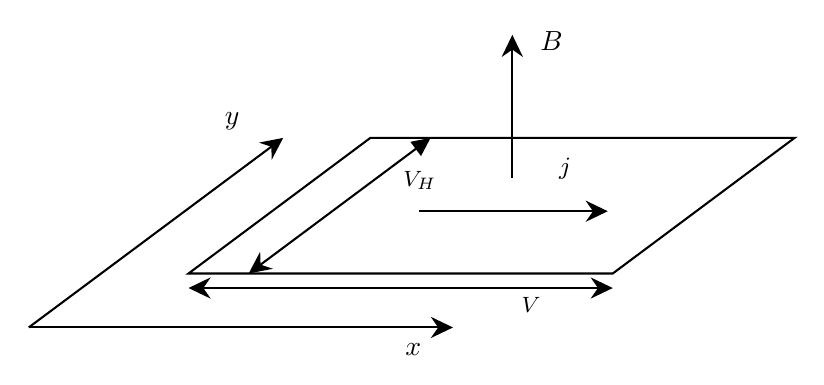
\begin{tikzpicture}[x=0.75pt,y=0.75pt,yscale=-1,xscale=1]
%uncomment if require: \path (0,300); %set diagram left start at 0, and has height of 300
%Shape: Parallelogram [id:dp2081197711183893]
\draw   (241.6,115) -- (446,115) -- (358.4,180.33) -- (154,180.33) -- cycle ;
%Straight Lines [id:da3392856291541302] 
\draw    (268.2,116.79) -- (185.4,178.54) ;
\draw [shift={(183,180.33)}, rotate = 323.28] [fill={rgb, 255:red, 0; green, 0; blue, 0 }  ][line width=0.08]  [draw opacity=0] (10.72,-5.15) -- (0,0) -- (10.72,5.15) -- (7.12,0) -- cycle    ;
\draw [shift={(270.6,115)}, rotate = 143.28] [fill={rgb, 255:red, 0; green, 0; blue, 0 }  ][line width=0.08]  [draw opacity=0] (8.93,-4.29) -- (0,0) -- (8.93,4.29) -- cycle    ;
%Straight Lines [id:da4116693786329637] 
\draw    (197.19,116.79) -- (77,206.33) ;
\draw [shift={(199.6,115)}, rotate = 143.31] [fill={rgb, 255:red, 0; green, 0; blue, 0 }  ][line width=0.08]  [draw opacity=0] (10.72,-5.15) -- (0,0) -- (10.72,5.15) -- (7.12,0) -- cycle    ;
%Straight Lines [id:da17430270610068788] 
\draw    (157,187.33) -- (355.4,187.33) ;
\draw [shift={(358.4,187.33)}, rotate = 180] [fill={rgb, 255:red, 0; green, 0; blue, 0 }  ][line width=0.08]  [draw opacity=0] (10.72,-5.15) -- (0,0) -- (10.72,5.15) -- (7.12,0) -- cycle    ;
\draw [shift={(154,187.33)}, rotate = 0] [fill={rgb, 255:red, 0; green, 0; blue, 0 }  ][line width=0.08]  [draw opacity=0] (10.72,-5.15) -- (0,0) -- (10.72,5.15) -- (7.12,0) -- cycle    ;
%Straight Lines [id:da40457739049168495] 
\draw    (77,206.33) -- (278.4,206.33) ;
\draw [shift={(281.4,206.33)}, rotate = 180] [fill={rgb, 255:red, 0; green, 0; blue, 0 }  ][line width=0.08]  [draw opacity=0] (10.72,-5.15) -- (0,0) -- (10.72,5.15) -- (7.12,0) -- cycle    ;
%Straight Lines [id:da710748552808127] 
\draw    (265,150.33) -- (353,150.33) ;
\draw [shift={(356,150.33)}, rotate = 180] [fill={rgb, 255:red, 0; green, 0; blue, 0 }  ][line width=0.08]  [draw opacity=0] (10.72,-5.15) -- (0,0) -- (10.72,5.15) -- (7.12,0) -- cycle    ;
%Straight Lines [id:da5473058663731798] 
\draw    (310,134.33) -- (310,68.33) ;
\draw [shift={(310,65.33)}, rotate = 450] [fill={rgb, 255:red, 0; green, 0; blue, 0 }  ][line width=0.08]  [draw opacity=0] (10.72,-5.15) -- (0,0) -- (10.72,5.15) -- (7.12,0) -- cycle    ;


% Text Node
\draw (257,212.4) node [anchor=north west][inner sep=0.75pt]    {$x$};
% Text Node
\draw (170,101.4) node [anchor=north west][inner sep=0.75pt]    {$y$};
% Text Node
\draw (256,129.4) node [anchor=north west][inner sep=0.75pt]  [font=\footnotesize]  {$V_{H}$};
% Text Node
\draw (331,123.4) node [anchor=north west][inner sep=0.75pt]  [font=\small]  {$\ot{j}$};
% Text Node
\draw (322,62.4) node [anchor=north west][inner sep=0.75pt]    {$\ot{B}$};
% Text Node
\draw (313,190.4) node [anchor=north west][inner sep=0.75pt]  [font=\footnotesize]  {$V$};


\end{tikzpicture}
\end{center}
\begin{enumerate}[1) ]
    \item  Giả sử rằng mẫu bán dẫn là một tấm hình vuông có kích thước $W\times W$. Dòng điện là do sự chuyển động của các hạt mang điện dương mỗi hạt có điện tích là $e$, mật độ mặt của các hạt tải điện là $n$, và độ dẫn điện của bán dẫn là $\sigma$. Cũng có các điện tích âm do đó các điện tích trung hòa ở khắp mọi nơi ngoại trừ tại cạnh bên. Điện trường là đều trong chất bán dẫn. Một từ trường $B$ được đặt vào theo hướng vuông góc với tấm. Khi một điện áp $V$ được đặt vào tấm thì sẽ xuất hiện một điện áp $V_{H}$ giữa hai cạnh song song với dòng điện dọc theo trục $x$, ngoài ra dòng điện $\ot{j}$. Khi ở trạng thái ổn định đạt được, tìm hệ số Hall $R_{H}=\dfrac{V_{H}}{V}$. (Lưu ý rằng $\ot{j}$ là đại lượng chưa biết).
\end{enumerate}
Ngày nay nó còn được gọi là cấu trúc bán dẫn số, một hiệu ứng spin $-$ Hall cũng sẽ xảy ra. Hiệu ứng được kết hợp cùng với moment từ $\ot{m}$ của các hạt mang điện. Đối với cấu trúc hai chiều được biết rằng có một lực bổ sung $\ot{F_{R}}=\eta_{R}(\ot{m}\times\ot{v})$ (gọi là lực Rashba) sẽ tác dụng lên các hạt tải điện, ở đây $\ot{v}$ là vận tốc của các hạt tải trên mặt phẳng hai chiều $(X-Y)$, và $\eta_{R}$ là một hằng số. Moment từ $\ot{m}$ bị hạn chế chỉ hướng vuông góc với mặt phẳng, ví dụ như $\ot{m}=m\widehat{z}$. Không có từ trường bên ngoài. Bỏ qua tương tác giữa lưỡng cực từ với các hạt tải điện.
\begin{enumerate}[1)]
\setcounter{enumi}{1}
    \item Giả sử hạt một lần nữa là điện trường là đều và lực của nó dọc theo trục $x$ là mạnh hơn $\ot{F_{R}}$, tìm dòng điện chạy theo hướng $y$ theo điện áp $V$ và các thông số khác đã được đưa ra trong ý $(1)$. Các dòng điện đó liên quan đến $\ot{m}$ như thế nào? 
    \item Do va chạm với biên, các hạt tải với moment từ riêng sẽ mất cảm giác của chúng về hướng trong một khoảng "thời gian sống" $\tau$ sau khi chúng tới được biên. Hay nói các khác, mỗi giây có $\dfrac{n_{m}}{\tau}$ hạt tải mất hướng moment của chúng trong một đơn vị chiều dài của cạnh, ở đây $n_{m}$ là mật độ bề mặt của hạt tải vẫn duy trì hướng moment của chúng $(\pm \widehat{z})$. Tìm độ từ hóa $\ot{M}$ ở gần các cạnh.
\end{enumerate}
\end{vd}
\begin{loigiai}
\begin{enumerate}[1) ]
    \item
Ta có mật độ dòng điện
\[j=nev=\sigma E,\]
lại có
\[E=\dfrac{V}{W},\]
suy ra lực điện tác dụng lên electron là
\[F_{\mathrm{E}}=\dfrac{eV_{\mathrm{H}}}{W}.\]
Lực Lorentz tác dụng lên electron là $F_{\mathrm{B}}=eBv$.\\
Khi đạt trạng thái ổn định $F_{\mathrm{E}}=F_{\mathrm{B}}$.\\Từ đó có thể thu được
\[\dfrac{V_{\mathrm{H}}}{V}=\dfrac{B\sigma}{en}.\]
    \item Tính trung bình, một nửa các electron có spin hướng lên, một nửa có spin hướng xuống. Electron chuyển động dọc theo trục $X$ để cho
    \[j=j_{\mathrm{y}}+j_{-\mathrm{y}},\]
    nhưng
    \[\ot{j_{\mathrm{spin}}}\neq 0,\]
    $j_{\mathrm{spin}}$ thực sự là một dòng spin, không có dòng điện tích.
    \[j_{\mathrm{y}}=\sigma E_{\mathrm{y}}=\dfrac{\sigma F_{\mathrm{t}}}{e}=\dfrac{\sigma \eta_{\mathrm{R}}mv_{\mathrm{x}}}{e}=\dfrac{\sigma\eta_{\mathrm{R}}m}{e}\dfrac{\sigma V}{nem}=\dfrac{\sigma^2\eta_{\mathrm{R}}mV}{e^2nW}.\]
    Dòng điện hướng sang trái hoặc sang phải do spin hướng lên hoặc hướng xuống.
    \item Khi đạt đến trạng thái cân bằng ta có
    \[\dfrac{n_{\mathrm{m}}}{\tau}=\dfrac{j_{\mathrm{i}}}{e},\]
    Do đó độ từ hóa khi đó sẽ là
    \[M=n_{\mathrm{m}}m=\dfrac{\sigma^2\eta_{\mathrm{R}}m^2\tau V}{Wne^3}.\]
\end{enumerate}
\end{loigiai}

\begin{vd}[Tấm điện môi di chuyển]
Một tấm điện môi phẳng lớn có độ dày $d$ và hẳng số điện môi $\varepsilon$ được di chuyển dọc theo trục $x$ ở tốc độ $v$. Mặt phẳng là vuông góc với trục $y$. Một từ trường có độ lớn $B$ được tác dụng theo hướng $z$. Tìm mật độ điện tích bề mặt trên hai bề mặt lớn của tấm, và điện trường trong tấm.
\begin{center}
    

\tikzset{every picture/.style={line width=0.75pt}} %set default line width to 0.75pt        

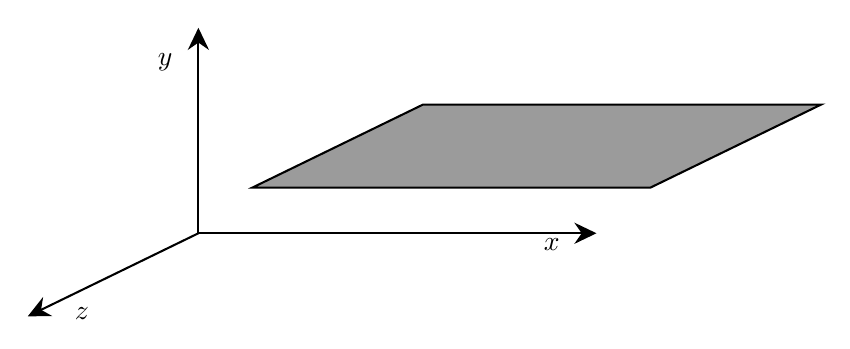
\begin{tikzpicture}[x=0.75pt,y=0.75pt,yscale=-1,xscale=1]
%uncomment if require: \path (0,300); %set diagram left start at 0, and has height of 300

%Shape: Parallelogram [id:dp06277634841378132] 
\draw  [fill={rgb, 255:red, 155; green, 155; blue, 155 }  ,fill opacity=1 ] (313.2,138.33) -- (505,138.33) -- (422.8,178.33) -- (231,178.33) -- cycle ;
%Straight Lines [id:da5182146849521212] 
\draw    (205,200.33) -- (393.8,200.33) ;
\draw [shift={(396.8,200.33)}, rotate = 180] [fill={rgb, 255:red, 0; green, 0; blue, 0 }  ][line width=0.08]  [draw opacity=0] (10.72,-5.15) -- (0,0) -- (10.72,5.15) -- (7.12,0) -- cycle    ;
%Straight Lines [id:da7214469395745302] 
\draw    (205,200.33) -- (125.5,239.02) ;
\draw [shift={(122.8,240.33)}, rotate = 334.05] [fill={rgb, 255:red, 0; green, 0; blue, 0 }  ][line width=0.08]  [draw opacity=0] (10.72,-5.15) -- (0,0) -- (10.72,5.15) -- (7.12,0) -- cycle    ;
%Straight Lines [id:da6293773454295502] 
\draw    (205,200.33) -- (205,104.33) ;
\draw [shift={(205,101.33)}, rotate = 450] [fill={rgb, 255:red, 0; green, 0; blue, 0 }  ][line width=0.08]  [draw opacity=0] (10.72,-5.15) -- (0,0) -- (10.72,5.15) -- (7.12,0) -- cycle    ;

% Text Node
\draw (370,201.4) node [anchor=north west][inner sep=0.75pt]    {$x$};
% Text Node
\draw (184,112.4) node [anchor=north west][inner sep=0.75pt]    {$y$};
% Text Node
\draw (144,234.4) node [anchor=north west][inner sep=0.75pt]    {$z$};


\end{tikzpicture}
\end{center}
\end{vd}
\begin{loigiai}
Mỗi đơn vị điện tích trong tấm chịu tác dụng của lực Lorentz $-vB\ot{y_0}$.\\
Bài toán là sau đó giống như một tấm điện môi đặt giữa hai tấm dẫn song song mang mật độ điện tích bề mặt $\pm\sigma$, và $\dfrac{\sigma}{\varepsilon_0}=vB$. Trong trường hợp như vậy, độ điện dịch là
\[D=\sigma\cdot P=D-\varepsilon_0E=D-\dfrac{D}{\varepsilon}=\varepsilon_0vB\left(\dfrac{\varepsilon-1}{\varepsilon}\right).\]
Cuối cùng, điện tích mặt liên kết là $\sigma_{b}=P=\varepsilon_0vB\left(\dfrac{\varepsilon-1}{\varepsilon}\right)$. Bề mặt phía trên mang điện tích liên kết dương, và bề mặt dưới mang điện tích liên kết âm.\\
Điện trường là $\ot{E}=\dfrac{\sigma_{b}}{\varepsilon_0}\ot{y_0}=vB\left(\dfrac{\varepsilon-1}{\varepsilon}\right)\ot{y_0}$, hướng dọc theo trục $y$ (ngược với hướng của lực Lorentz).
\end{loigiai}

\begin{vd}[Quan sát từ trường]
    Một vòng dẫn có bán kính $R$ mang dòng điện lớn $I$. Vòng dây nằm yên trong mặt phẳng $xy$ với tâm của nó là $(0,0,0)$. Một quan sát viên tiến đến chiếc vòng song song với trục $z$ với vận tốc $v$ và đo điện trường cách trục một khoảng $r$. Giả sử rằng $v\ll c$ và $r \ll R$.
    \begin{enumerate}[1)]
        \item Tìm phương và độ lớn của từ trường $B(z)$ trên trục $z$ trong hệ quy chiếu đứng yên.
        \item Ước lượng độ lớn và hướng của điện trường $E(z,r)$ mà người quan sát đo được khi người đó ở cách mặt phẳng vòng một khoảng $z$.
    \end{enumerate} 
\end{vd}

\begin{loigiai}
    \begin{enumerate}[1)]
        \item Theo định luật Bio $-$ Savart, mọi phần tử của vòng có chiều dài và hướng $\mathrm{d}\ot{l}$ đều tạo ra từ trường
        \[{\mathrm{d}}\overrightarrow B  = \frac{{{\mu _0}Im{\mathrm{d}}\overrightarrow l \overrightarrow a }}{{4\pi {a^3}}}.\]
        Theo đối xứng, thành phần từ trường vuông góc với trục $z$ triệt tiêu lẫn nhau. Vì vậy, từ trường có hướng dọc theo trục $z$.
        \[B(z) = \dfrac{\mu_0 \times 2\pi R \sin \alpha}{4\pi \left(z^2+R^2\right)}=\dfrac{\mu_0IR^2}{2\left(z^2+R^2\right)^{3/2}}.\]
        \item Điện trường đo được bởi một quan sát viên phải cùng hướng với lực Lorentz tác dụng lên quan sát viên trong hệ quy chiếu phòng thí nghiệm. Do đó đường sức của điện trường là những đường tròn quanh trục. Bây giờ chúng ta có thể áp dụng định luật cảm ứng của Faraday cho một vòng tròn như vậy, khi nó tiến gần đến vòng, tổng suất điện động là: 
        \[E(z,r)\times 2\pi r= \dot\Phi=-\dfrac{\mathrm{d}\Phi}{\mathrm{d}z}v \approx -\dfrac{\mathrm{d}}{\mathrm{d}z}B(z)\times \pi r^2 \times v\]
        \[\rt E(z,r)=-\dfrac{rv}{2}B'(z)=\dfrac{3\mu_0IrR^2vz}{4\left(z^2+R^2\right)^{5/2}}\]
    \end{enumerate}
\end{loigiai}

\begin{vd}[Ống từ]
%Prob 1C IPhO 2012
Xét một ống hình trụ làm bằng một vật liệu siêu dẫn. Độ dài của ống là $l$ và bán kính trong của ống là $r$; ta luôn có $l \gg r$. Tâm điểm ống trùng với gốc toạ độ, và trục của ống trùng với trục $z$. Có một từ thông $\Phi$ qua mặt cắt ngang trung tâm của ống, $z=0, x^{2}+y^{2} < r^{2}$. Siêu dẫn là vật liệu mà từ trường bị đẩy ra khỏi khối vật liệu (từ trường bằng không bên trong vật siêu dẫn).
\begin{center}


% Gradient Info
  
\tikzset {_0j96cq30i/.code = {\pgfsetadditionalshadetransform{ \pgftransformshift{\pgfpoint{0 bp } { 0 bp }  }  \pgftransformrotate{0 }  \pgftransformscale{2 }  }}}
\pgfdeclarehorizontalshading{_vok16xrsk}{150bp}{rgb(0bp)=(0.5,0.5,0.5);
rgb(37.5bp)=(0.5,0.5,0.5);
rgb(42.05357142857143bp)=(1,1,1);
rgb(50bp)=(1,1,1);
rgb(62.5bp)=(0.51,0.49,0.49);
rgb(100bp)=(0.51,0.49,0.49)}

% Pattern Info
 
\tikzset{
pattern size/.store in=\mcSize, 
pattern size = 5pt,
pattern thickness/.store in=\mcThickness, 
pattern thickness = 0.3pt,
pattern radius/.store in=\mcRadius, 
pattern radius = 1pt}
\makeatletter
\pgfutil@ifundefined{pgf@pattern@name@_raq4i4k97}{
\pgfdeclarepatternformonly[\mcThickness,\mcSize]{_raq4i4k97}
{\pgfqpoint{0pt}{0pt}}
{\pgfpoint{\mcSize}{\mcSize}}
{\pgfpoint{\mcSize}{\mcSize}}
{
\pgfsetcolor{\tikz@pattern@color}
\pgfsetlinewidth{\mcThickness}
\pgfpathmoveto{\pgfqpoint{0pt}{\mcSize}}
\pgfpathlineto{\pgfpoint{\mcSize+\mcThickness}{-\mcThickness}}
\pgfpathmoveto{\pgfqpoint{0pt}{0pt}}
\pgfpathlineto{\pgfpoint{\mcSize+\mcThickness}{\mcSize+\mcThickness}}
\pgfusepath{stroke}
}}
\makeatother
\tikzset{every picture/.style={line width=0.75pt}} %set default line width to 0.75pt        

\begin{tikzpicture}[x=0.75pt,y=0.75pt,yscale=-1,xscale=1]
%uncomment if require: \path (0,476); %set diagram left start at 0, and has height of 476

%Shape: Can [id:dp9073202998352221] 
\path  [shading=_vok16xrsk,_0j96cq30i] (265.66,67.67) -- (265.66,349.55) .. controls (265.66,353.57) and (254.82,356.82) .. (241.45,356.82) .. controls (228.07,356.82) and (217.23,353.57) .. (217.23,349.55) -- (217.23,67.67) .. controls (217.23,63.66) and (228.07,60.41) .. (241.45,60.41) .. controls (254.82,60.41) and (265.66,63.66) .. (265.66,67.67) .. controls (265.66,71.69) and (254.82,74.94) .. (241.45,74.94) .. controls (228.07,74.94) and (217.23,71.69) .. (217.23,67.67) ; % for fading 
 \draw   (265.66,67.67) -- (265.66,349.55) .. controls (265.66,353.57) and (254.82,356.82) .. (241.45,356.82) .. controls (228.07,356.82) and (217.23,353.57) .. (217.23,349.55) -- (217.23,67.67) .. controls (217.23,63.66) and (228.07,60.41) .. (241.45,60.41) .. controls (254.82,60.41) and (265.66,63.66) .. (265.66,67.67) .. controls (265.66,71.69) and (254.82,74.94) .. (241.45,74.94) .. controls (228.07,74.94) and (217.23,71.69) .. (217.23,67.67) ; % for border 

%Straight Lines [id:da2345937464732395] 
\draw    (241.45,74.94) -- (241.45,26.68) ;
\draw [shift={(241.45,23.68)}, rotate = 450] [fill={rgb, 255:red, 0; green, 0; blue, 0 }  ][line width=0.08]  [draw opacity=0] (10.72,-5.15) -- (0,0) -- (10.72,5.15) -- (7.12,0) -- cycle    ;
%Straight Lines [id:da32319017911629233] 
\draw    (241.45,356.82) -- (241.45,373.72) ;
%Straight Lines [id:da8220104477065213] 
\draw    (265.55,213.65) -- (280.21,213.65) ;
\draw [shift={(283.21,213.65)}, rotate = 180] [fill={rgb, 255:red, 0; green, 0; blue, 0 }  ][line width=0.08]  [draw opacity=0] (10.72,-5.15) -- (0,0) -- (10.72,5.15) -- (7.12,0) -- cycle    ;
%Straight Lines [id:da9619520904426937] 
\draw    (238.68,215.6) -- (205.62,241.54) ;
\draw [shift={(203.26,243.39)}, rotate = 321.89] [fill={rgb, 255:red, 0; green, 0; blue, 0 }  ][line width=0.08]  [draw opacity=0] (10.72,-5.15) -- (0,0) -- (10.72,5.15) -- (7.12,0) -- cycle    ;
%Straight Lines [id:da08678102869582371] 
\draw    (196.43,213.65) -- (217.13,213.65) ;
%Straight Lines [id:da1612752830968902] 
\draw [color={rgb, 255:red, 21; green, 72; blue, 132 }  ,draw opacity=1 ][line width=2.25]    (315.71,75.04) -- (315.71,354.87) ;
%Straight Lines [id:da7785637964939405] 
\draw [color={rgb, 255:red, 21; green, 72; blue, 132 }  ,draw opacity=1 ][line width=2.25]    (363.49,75.04) -- (363.49,354.87) ;
%Shape: Ellipse [id:dp34115363375590846] 
\draw  [color={rgb, 255:red, 21; green, 72; blue, 132 }  ,draw opacity=1 ][line width=2.25]  (217.23,67.67) .. controls (217.23,63.66) and (228.07,60.41) .. (241.45,60.41) .. controls (254.82,60.41) and (265.66,63.66) .. (265.66,67.67) .. controls (265.66,71.69) and (254.82,74.94) .. (241.45,74.94) .. controls (228.07,74.94) and (217.23,71.69) .. (217.23,67.67) -- cycle ;
%Shape: Ellipse [id:dp5975693393923946] 
\draw  [color={rgb, 255:red, 0; green, 0; blue, 0 }  ,draw opacity=1 ][pattern=_raq4i4k97,pattern size=6pt,pattern thickness=0.75pt,pattern radius=0pt, pattern color={rgb, 255:red, 0; green, 0; blue, 0}] (217.13,213.65) .. controls (217.13,209.64) and (227.97,206.39) .. (241.34,206.39) .. controls (254.71,206.39) and (265.55,209.64) .. (265.55,213.65) .. controls (265.55,217.66) and (254.71,220.92) .. (241.34,220.92) .. controls (227.97,220.92) and (217.13,217.66) .. (217.13,213.65) -- cycle ;
%Straight Lines [id:da6215766219137793] 
\draw    (301.95,214.3) -- (396.46,214.3) ;
\draw [shift={(399.46,214.3)}, rotate = 180] [fill={rgb, 255:red, 0; green, 0; blue, 0 }  ][line width=0.08]  [draw opacity=0] (10.72,-5.15) -- (0,0) -- (10.72,5.15) -- (7.12,0) -- cycle    ;
%Shape: Ellipse [id:dp06972730202487609] 
\draw  [color={rgb, 255:red, 0; green, 0; blue, 0 }  ,draw opacity=0 ][fill={rgb, 255:red, 208; green, 2; blue, 27 }  ,fill opacity=1 ] (337.92,214.34) .. controls (337.92,213.44) and (338.65,212.72) .. (339.55,212.72) .. controls (340.44,212.72) and (341.17,213.44) .. (341.17,214.34) .. controls (341.17,215.24) and (340.44,215.97) .. (339.55,215.97) .. controls (338.65,215.97) and (337.92,215.24) .. (337.92,214.34) -- cycle ;
%Shape: Ellipse [id:dp04603211008785135] 
\draw  [color={rgb, 255:red, 0; green, 0; blue, 0 }  ,draw opacity=0 ][fill={rgb, 255:red, 208; green, 2; blue, 27 }  ,fill opacity=1 ] (347.45,214.3) .. controls (347.45,213.4) and (348.18,212.68) .. (349.08,212.68) .. controls (349.98,212.68) and (350.7,213.4) .. (350.7,214.3) .. controls (350.7,215.2) and (349.98,215.93) .. (349.08,215.93) .. controls (348.18,215.93) and (347.45,215.2) .. (347.45,214.3) -- cycle ;
%Shape: Ellipse [id:dp08243184704905993] 
\draw  [color={rgb, 255:red, 0; green, 0; blue, 0 }  ,draw opacity=0 ][fill={rgb, 255:red, 208; green, 2; blue, 27 }  ,fill opacity=1 ] (354.58,214.25) .. controls (354.58,213.36) and (355.31,212.63) .. (356.21,212.63) .. controls (357.11,212.63) and (357.83,213.36) .. (357.83,214.25) .. controls (357.83,215.15) and (357.11,215.88) .. (356.21,215.88) .. controls (355.31,215.88) and (354.58,215.15) .. (354.58,214.25) -- cycle ;
%Shape: Ellipse [id:dp8358277433819097] 
\draw  [color={rgb, 255:red, 0; green, 0; blue, 0 }  ,draw opacity=0 ][fill={rgb, 255:red, 208; green, 2; blue, 27 }  ,fill opacity=1 ] (329.41,214.34) .. controls (329.41,213.44) and (330.14,212.72) .. (331.04,212.72) .. controls (331.93,212.72) and (332.66,213.44) .. (332.66,214.34) .. controls (332.66,215.24) and (331.93,215.97) .. (331.04,215.97) .. controls (330.14,215.97) and (329.41,215.24) .. (329.41,214.34) -- cycle ;
%Shape: Ellipse [id:dp12453488097442245] 
\draw  [color={rgb, 255:red, 0; green, 0; blue, 0 }  ,draw opacity=0 ][fill={rgb, 255:red, 208; green, 2; blue, 27 }  ,fill opacity=1 ] (321.61,214.34) .. controls (321.61,213.44) and (322.34,212.72) .. (323.24,212.72) .. controls (324.13,212.72) and (324.86,213.44) .. (324.86,214.34) .. controls (324.86,215.24) and (324.13,215.97) .. (323.24,215.97) .. controls (322.34,215.97) and (321.61,215.24) .. (321.61,214.34) -- cycle ;
%Straight Lines [id:da04272554723886168] 
\draw    (345.94,78.04) -- (345.94,351.87) ;
\draw [shift={(345.94,354.87)}, rotate = 270] [fill={rgb, 255:red, 0; green, 0; blue, 0 }  ][line width=0.08]  [draw opacity=0] (10.72,-5.15) -- (0,0) -- (10.72,5.15) -- (7.12,0) -- cycle    ;
\draw [shift={(345.94,75.04)}, rotate = 90] [fill={rgb, 255:red, 0; green, 0; blue, 0 }  ][line width=0.08]  [draw opacity=0] (10.72,-5.15) -- (0,0) -- (10.72,5.15) -- (7.12,0) -- cycle    ;
%Straight Lines [id:da4730485341493289] 
\draw    (339.44,29.12) -- (339.44,367.38) ;
\draw [shift={(339.44,26.12)}, rotate = 90] [fill={rgb, 255:red, 0; green, 0; blue, 0 }  ][line width=0.08]  [draw opacity=0] (10.72,-5.15) -- (0,0) -- (10.72,5.15) -- (7.12,0) -- cycle    ;
%Straight Lines [id:da4859654190879201] 
\draw    (318.71,339.27) -- (360.49,339.27) ;
\draw [shift={(363.49,339.27)}, rotate = 180] [fill={rgb, 255:red, 0; green, 0; blue, 0 }  ][line width=0.08]  [draw opacity=0] (10.72,-5.15) -- (0,0) -- (10.72,5.15) -- (7.12,0) -- cycle    ;
\draw [shift={(315.71,339.27)}, rotate = 0] [fill={rgb, 255:red, 0; green, 0; blue, 0 }  ][line width=0.08]  [draw opacity=0] (10.72,-5.15) -- (0,0) -- (10.72,5.15) -- (7.12,0) -- cycle    ;
%Straight Lines [id:da2615178758144112] 
\draw  [dash pattern={on 4.5pt off 4.5pt}]  (315.71,354.87) -- (363.49,354.87) ;
%Straight Lines [id:da8868897877516484] 
\draw  [dash pattern={on 4.5pt off 4.5pt}]  (315.71,75.04) -- (363.49,75.04) ;

% Text Node
\draw (248.28,18.2) node [anchor=north west][inner sep=0.75pt]    {$z$};
% Text Node
\draw (186.86,228.8) node [anchor=north west][inner sep=0.75pt]    {$x$};
% Text Node
\draw (279.16,189.15) node [anchor=north west][inner sep=0.75pt]    {$y$};
% Text Node
\draw (233.62,186.23) node [anchor=north west][inner sep=0.75pt]    {$\Phi$};
% Text Node
\draw (393.56,180.25) node [anchor=north west][inner sep=0.75pt]    {$y$};
% Text Node
\draw (347.09,19.82) node [anchor=north west][inner sep=0.75pt]    {$z$};
% Text Node
\draw (322.43,319.16) node [anchor=north west][inner sep=0.75pt]    {$2r$};
% Text Node
\draw (295.29,279.75) node [anchor=north west][inner sep=0.75pt]  [color={rgb, 255:red, 21; green, 72; blue, 132 }  ,opacity=1 ,rotate=-270] [align=left] {Thành trụ siêu dẫn};
% Text Node
\draw (321.95,293.61) node [anchor=north west][inner sep=0.75pt]  [rotate=-270] [align=left] {Mặt cắt dọc để vẽ trường};
% Text Node
\draw (349.69,188.18) node [anchor=north west][inner sep=0.75pt]    {$l$};
\end{tikzpicture}
\end{center}
\begin{enumerate}[1)]
    \item Hãy phác họa năm đường sức từ; các đường này đi qua năm chấm được đánh dấu trên mặt cắt đi qua trục của ống. 
    \item Hãy tìm lực căng $T$ hướng theo trục $z$ ở giữa ống (tức là lực mà hai nửa của ống với $z>0$ và $z<0$ tác dụng lên nhau).
    \item Bây giờ, có thêm một ống nữa giống hệt và song song với ống ban đầu. Ống thứ hai có từ trường theo chiều ngược lại, và có tâm ở $y=l, x=z=0$ (tức là hai ống lập thành hai cạnh đối diện của một hình vuông). Hãy xác định lực tương tác từ $F$ giữa hai ống.
\end{enumerate}


\begin{center}


% Gradient Info
  
\tikzset {_awtnk2ubg/.code = {\pgfsetadditionalshadetransform{ \pgftransformshift{\pgfpoint{0 bp } { 0 bp }  }  \pgftransformrotate{0 }  \pgftransformscale{2 }  }}}
\pgfdeclarehorizontalshading{_jfe9j5j4u}{150bp}{rgb(0bp)=(0.5,0.5,0.5);
rgb(37.5bp)=(0.5,0.5,0.5);
rgb(42.05357142857143bp)=(1,1,1);
rgb(50bp)=(1,1,1);
rgb(62.5bp)=(0.51,0.49,0.49);
rgb(100bp)=(0.51,0.49,0.49)}

% Gradient Info
  
\tikzset {_f4cd73l13/.code = {\pgfsetadditionalshadetransform{ \pgftransformshift{\pgfpoint{0 bp } { 0 bp }  }  \pgftransformrotate{0 }  \pgftransformscale{2 }  }}}
\pgfdeclarehorizontalshading{_qngu2ta4z}{150bp}{rgb(0bp)=(0.5,0.5,0.5);
rgb(37.5bp)=(0.5,0.5,0.5);
rgb(42.05357142857143bp)=(1,1,1);
rgb(50bp)=(1,1,1);
rgb(62.5bp)=(0.51,0.49,0.49);
rgb(100bp)=(0.51,0.49,0.49)}

% Gradient Info
  
\tikzset {_7zc1sf1iu/.code = {\pgfsetadditionalshadetransform{ \pgftransformshift{\pgfpoint{0 bp } { 0 bp }  }  \pgftransformrotate{-90 }  \pgftransformscale{2 }  }}}
\pgfdeclarehorizontalshading{_nius93n0k}{150bp}{rgb(0bp)=(0.23,0.46,0.73);
rgb(37.5bp)=(0.23,0.46,0.73);
rgb(62.5bp)=(0.6,0.14,0.14);
rgb(100bp)=(0.6,0.14,0.14)}
\tikzset{_fpvm79qbs/.code = {\pgfsetadditionalshadetransform{\pgftransformshift{\pgfpoint{0 bp } { 0 bp }  }  \pgftransformrotate{-90 }  \pgftransformscale{2 } }}}
\pgfdeclarehorizontalshading{_emnp0vw3r} {150bp} {color(0bp)=(transparent!0);
color(37.5bp)=(transparent!0);
color(62.5bp)=(transparent!10);
color(100bp)=(transparent!10) } 
\pgfdeclarefading{_740hf4uvr}{\tikz \fill[shading=_emnp0vw3r,_fpvm79qbs] (0,0) rectangle (50bp,50bp); } 

% Gradient Info
  
\tikzset {_av5scdeu2/.code = {\pgfsetadditionalshadetransform{ \pgftransformshift{\pgfpoint{0 bp } { 0 bp }  }  \pgftransformrotate{-270 }  \pgftransformscale{2 }  }}}
\pgfdeclarehorizontalshading{_qo9gkk403}{150bp}{rgb(0bp)=(0.23,0.46,0.73);
rgb(37.5bp)=(0.23,0.46,0.73);
rgb(62.5bp)=(0.6,0.14,0.14);
rgb(100bp)=(0.6,0.14,0.14)}
\tikzset{_p72kr0ay4/.code = {\pgfsetadditionalshadetransform{\pgftransformshift{\pgfpoint{0 bp } { 0 bp }  }  \pgftransformrotate{-270 }  \pgftransformscale{2 } }}}
\pgfdeclarehorizontalshading{_1utn2qea4} {150bp} {color(0bp)=(transparent!0);
color(37.5bp)=(transparent!0);
color(62.5bp)=(transparent!10);
color(100bp)=(transparent!10) } 
\pgfdeclarefading{_irz0xhpjt}{\tikz \fill[shading=_1utn2qea4,_p72kr0ay4] (0,0) rectangle (50bp,50bp); } 
\tikzset{every picture/.style={line width=0.75pt}} %set default line width to 0.75pt        

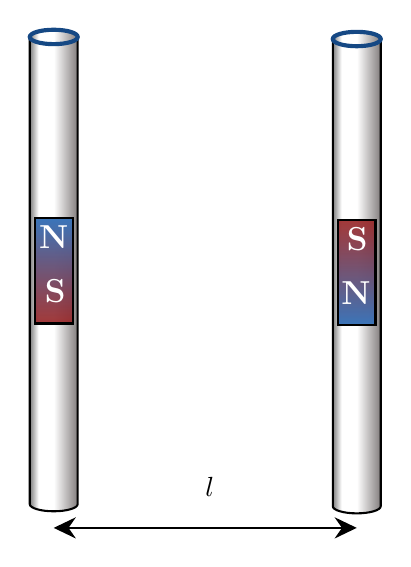
\begin{tikzpicture}[x=0.75pt,y=0.75pt,yscale=-1,xscale=1]
%uncomment if require: \path (0,458); %set diagram left start at 0, and has height of 458

%Shape: Can [id:dp007819295205010013] 
\path  [shading=_jfe9j5j4u,_awtnk2ubg] (242,80.46) -- (242,305.54) .. controls (242,307.45) and (236.83,309) .. (230.45,309) .. controls (224.07,309) and (218.9,307.45) .. (218.9,305.54) -- (218.9,80.46) .. controls (218.9,78.55) and (224.07,77) .. (230.45,77) .. controls (236.83,77) and (242,78.55) .. (242,80.46) .. controls (242,82.38) and (236.83,83.93) .. (230.45,83.93) .. controls (224.07,83.93) and (218.9,82.38) .. (218.9,80.46) ; % for fading 
 \draw   (242,80.46) -- (242,305.54) .. controls (242,307.45) and (236.83,309) .. (230.45,309) .. controls (224.07,309) and (218.9,307.45) .. (218.9,305.54) -- (218.9,80.46) .. controls (218.9,78.55) and (224.07,77) .. (230.45,77) .. controls (236.83,77) and (242,78.55) .. (242,80.46) .. controls (242,82.38) and (236.83,83.93) .. (230.45,83.93) .. controls (224.07,83.93) and (218.9,82.38) .. (218.9,80.46) ; % for border 

%Shape: Ellipse [id:dp9186541993707484] 
\draw  [color={rgb, 255:red, 21; green, 72; blue, 132 }  ,draw opacity=1 ][line width=1.5]  (218.9,80.46) .. controls (218.9,78.55) and (224.07,77) .. (230.45,77) .. controls (236.83,77) and (242,78.55) .. (242,80.46) .. controls (242,82.38) and (236.83,83.93) .. (230.45,83.93) .. controls (224.07,83.93) and (218.9,82.38) .. (218.9,80.46) -- cycle ;
%Shape: Can [id:dp2898523859953672] 
\path  [shading=_qngu2ta4z,_f4cd73l13] (388,81.46) -- (388,306.54) .. controls (388,308.45) and (382.83,310) .. (376.45,310) .. controls (370.07,310) and (364.9,308.45) .. (364.9,306.54) -- (364.9,81.46) .. controls (364.9,79.55) and (370.07,78) .. (376.45,78) .. controls (382.83,78) and (388,79.55) .. (388,81.46) .. controls (388,83.38) and (382.83,84.93) .. (376.45,84.93) .. controls (370.07,84.93) and (364.9,83.38) .. (364.9,81.46) ; % for fading 
 \draw   (388,81.46) -- (388,306.54) .. controls (388,308.45) and (382.83,310) .. (376.45,310) .. controls (370.07,310) and (364.9,308.45) .. (364.9,306.54) -- (364.9,81.46) .. controls (364.9,79.55) and (370.07,78) .. (376.45,78) .. controls (382.83,78) and (388,79.55) .. (388,81.46) .. controls (388,83.38) and (382.83,84.93) .. (376.45,84.93) .. controls (370.07,84.93) and (364.9,83.38) .. (364.9,81.46) ; % for border 

%Shape: Ellipse [id:dp4510250887340068] 
\draw  [color={rgb, 255:red, 21; green, 72; blue, 132 }  ,draw opacity=1 ][line width=1.5]  (364.9,81.46) .. controls (364.9,79.55) and (370.07,78) .. (376.45,78) .. controls (382.83,78) and (388,79.55) .. (388,81.46) .. controls (388,83.38) and (382.83,84.93) .. (376.45,84.93) .. controls (370.07,84.93) and (364.9,83.38) .. (364.9,81.46) -- cycle ;
%Straight Lines [id:da6466501046274797] 
\draw    (233.45,317) -- (373.45,317) ;
\draw [shift={(376.45,317)}, rotate = 180] [fill={rgb, 255:red, 0; green, 0; blue, 0 }  ][line width=0.08]  [draw opacity=0] (10.72,-5.15) -- (0,0) -- (10.72,5.15) -- (7.12,0) -- cycle    ;
\draw [shift={(230.45,317)}, rotate = 0] [fill={rgb, 255:red, 0; green, 0; blue, 0 }  ][line width=0.08]  [draw opacity=0] (10.72,-5.15) -- (0,0) -- (10.72,5.15) -- (7.12,0) -- cycle    ;
%Shape: Rectangle [id:dp24857948347045467] 
\path  [shading=_nius93n0k,_7zc1sf1iu,path fading= _740hf4uvr ,fading transform={xshift=2}] (221.38,167.85) -- (239.64,167.85) -- (239.64,218.52) -- (221.38,218.52) -- cycle ; % for fading 
 \draw   (221.38,167.85) -- (239.64,167.85) -- (239.64,218.52) -- (221.38,218.52) -- cycle ; % for border 

%Shape: Rectangle [id:dp9776464464035521] 
\path  [shading=_qo9gkk403,_av5scdeu2,path fading= _irz0xhpjt ,fading transform={xshift=2}] (367.2,168.67) -- (385.47,168.67) -- (385.47,219.33) -- (367.2,219.33) -- cycle ; % for fading 
 \draw   (367.2,168.67) -- (385.47,168.67) -- (385.47,219.33) -- (367.2,219.33) -- cycle ; % for border 


% Text Node
\draw (302,291.07) node [anchor=north west][inner sep=0.75pt]    {$l$};
% Text Node
\draw (221.88,170) node [anchor=north west][inner sep=0.75pt]  [font=\large,color={rgb, 255:red, 255; green, 255; blue, 255 }  ,opacity=1 ]  {$\mathbf{N}$};
% Text Node
\draw (224.68,196.17) node [anchor=north west][inner sep=0.75pt]  [font=\large,color={rgb, 255:red, 255; green, 255; blue, 255 }  ,opacity=1 ]  {$\mathbf{S}$};
% Text Node
\draw (367.59,196.98) node [anchor=north west][inner sep=0.75pt]  [font=\large,color={rgb, 255:red, 255; green, 255; blue, 255 }  ,opacity=1 ]  {$\mathbf{N}$};
% Text Node
\draw (370.21,171.04) node [anchor=north west][inner sep=0.75pt]  [font=\large,color={rgb, 255:red, 255; green, 255; blue, 255 }  ,opacity=1 ]  {$\mathbf{S}$};
\end{tikzpicture}

\end{center}
\end{vd}
\begin{loigiai}
\begin{enumerate}[1)]
    \item Do các ống siêu dẫn, các đường sức từ không thể xuyên qua thành trụ, do đó, thông lượng không đổi dọc theo ống. Đối với một đường sức khép kín ở bên trong ống, không có lưu số của từ trường, do đó các đường sức của từ trường không thể bị cong và từ trường cần phải đồng nhất. Các đường sức từ ở gần phía bên ngoài ống, tương tự như một ống dây solenoid.
    \begin{center}
\tikzset{every picture/.style={line width=0.75pt}} %set default line width to 0.75pt        

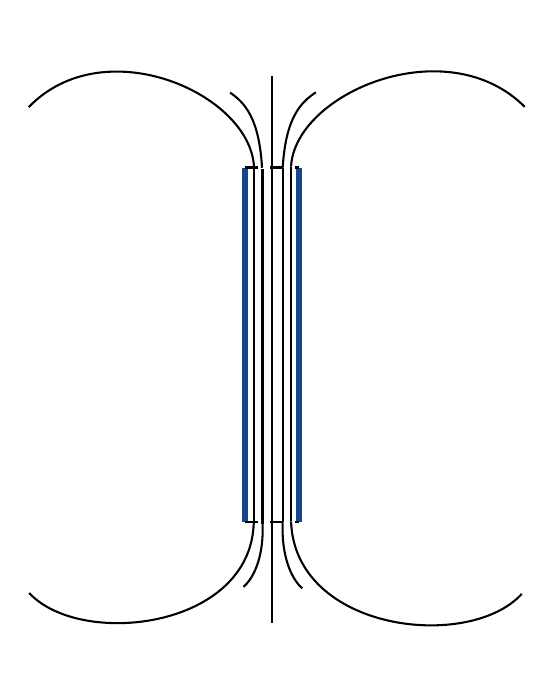
\begin{tikzpicture}[x=0.75pt,y=0.75pt,yscale=-1,xscale=1]
%uncomment if require: \path (0,486); %set diagram left start at 0, and has height of 486

%Straight Lines [id:da6553941977266136] 
\draw    (380.3,55.96) -- (380.3,319.34) ;
%Straight Lines [id:da20807427921017485] 
\draw    (371.4,100.64) -- (371.4,271.56) ;
%Straight Lines [id:da09600028335803557] 
\draw    (375.65,100.64) -- (375.65,271.56) ;
%Straight Lines [id:da2317987383186828] 
\draw    (380.3,56.08) -- (380.3,319.46) ;
%Straight Lines [id:da9566806595393609] 
\draw    (385.37,100.02) -- (385.37,270.94) ;
%Straight Lines [id:da7102809161790751] 
\draw    (389.39,99.59) -- (389.39,270.51) ;
%Straight Lines [id:da8918361849245788] 
\draw [color={rgb, 255:red, 21; green, 72; blue, 132 }  ,draw opacity=1 ][line width=2.25]    (367.29,100.02) -- (367.29,270.94) ;
%Straight Lines [id:da6221347119396883] 
\draw [color={rgb, 255:red, 21; green, 72; blue, 132 }  ,draw opacity=1 ][line width=2.25]    (393.36,100.02) -- (393.36,270.94) ;
%Straight Lines [id:da49533431081663504] 
\draw  [dash pattern={on 4.5pt off 4.5pt}]  (367.29,270.94) -- (393.36,270.94) ;
%Straight Lines [id:da09584577214604817] 
\draw  [dash pattern={on 4.5pt off 4.5pt}]  (367.29,100.02) -- (393.36,100.02) ;
%Curve Lines [id:da18554010631590634] 
\draw    (385.37,100.02) .. controls (386.85,75.88) and (394.09,68.64) .. (401.33,63.81) ;
%Curve Lines [id:da8595614909451721] 
\draw    (394.81,302.81) .. controls (389.02,297.74) and (384.67,286.15) .. (385.37,270.94) ;
%Curve Lines [id:da7406026790407734] 
\draw    (389.39,99.59) .. controls (391.19,64.29) and (464.34,33.15) .. (502,70.81) ;
%Curve Lines [id:da6687731995487289] 
\draw    (500.55,305.46) .. controls (475.2,333.23) and (391.19,323.57) .. (389.39,270.51) ;
%Curve Lines [id:da4904141756796325] 
\draw    (375.41,100.14) .. controls (373.99,76) and (367.01,68.76) .. (360.03,63.93) ;
%Curve Lines [id:da7424205508205513] 
\draw    (371.53,99.71) .. controls (369.8,64.41) and (299.3,33.27) .. (263,70.93) ;
%Curve Lines [id:da2030810164939778] 
\draw    (366.46,302.08) .. controls (372.1,297.22) and (376.33,286.13) .. (375.65,271.56) ;
%Curve Lines [id:da416386997545346] 
\draw    (263.23,305.03) .. controls (287.9,331.62) and (369.65,322.37) .. (371.4,271.56) ;
\end{tikzpicture}
    \end{center}
    \item Chúng ta hãy xem xét sự thay đổi của năng lượng từ khi ống được kéo dài một lượng nhỏ $\Delta l$.\\
    \textbf{Lưu ý.} Từ thông qua ống được bảo toàn: bất kì sự thay đổi từ thông nào cũng sẽ sinh ra một suất điện động $\dfrac{\dd \Phi}{\dd t}$, và đối với vật liệu có điện trở suất bằng không, ta có một dòng điện vô hạn. Vì vậy, cảm ứng từ $B = \dfrac{\Phi}{\pi r^{2}}$. Mật độ năng lượng của từ trường là $\dfrac{B^{2}}{2 \mu_{0}}$. \\
    Do đó, sự thay đổi của năng lượng từ trường được tính như sau:
    \[\Delta W = \dfrac{B^{2}}{2 \mu_{0}} \pi r^{2} \Delta l = \dfrac{\Phi^{2}}{2 \mu_{0} \pi r^{2}} \Delta l.\]
    Sự gia tăng năng lượng này có được nhờ công của lực kéo dãn, $\Delta W = T \Delta l$. Do đó, lực căng là
    \[T = \dfrac{\Phi^{2}}{2 \mu_{0} \pi r^{2}}.\]  
    \item Bây giờ chúng ta hãy phân tích, sự thay đổi của năng lượng từ  khi một trong các ống được di chuyển một khoảng cách nhỏ. Từ trường bên trong các ống sẽ không đổi do bảo toàn từ thông, nhưng bên ngoài, từ trường sẽ bị thay đổi.\\
    Từ trường bên ngoài ống được xác định bởi điều kiện sau: không có lưu số của vector $\ot{B}$ (vì không có dòng điện nào bên ngoài ống); không có nguồn của các đường sức từ nào khác ngoài hai đầu của ống; mỗi đầu của ống là một nguồn của các đường dòng với một từ thông xác định $\pm \Phi$. \\
    Điều kiện này giống như điều kiện xác định điện trường của bốn điện tích $\pm Q$. Chúng ta biết rằng nếu khoảng cách giữa các điện tích lớn hơn nhiều so với kích thước hình học của một điện tích, các điện tích có thể được coi là điện tích điểm (điện trường gần các điện tích vẫn gần như không đổi, do đó sự đóng góp tương ứng vào sự thay đổi năng lượng điện trường tổng thể là không đáng kể).\\
    Do đó, chúng ta có thể kết luận rằng các đầu của ống có thể được coi là từ tích (đơn cực từ). Để tính toán lực giữa hai từ tích (đơn cực từ), chúng ta cần thiết lập sự tương ứng giữa các đại lượng từ và điện.\\
    Đối với hai điện tích $Q$ cách nhau bởi khoảng cách $a$, lực là 
    \[F=\dfrac{1}{4 \pi \varepsilon_{0}} \dfrac{Q^{2}}{a^{2}},\] 
    và tại vị trí của một điện tích, điện trường của điện tích còn lại có mật độ năng lượng 
    \[\omega = \dfrac{1}{32 \pi^2 \varepsilon_0 }\dfrac{Q^2}{a^4}.\]
    Do đó, ta có thể viết
    \[F = 8\pi \omega a^2.\]
    Đây là một biểu thức chung cho lực (đối với trường hợp các đường sức từ có cùng hình dạng với đường sức điện giữa hai điện tích trái dấu và bằng nhau về độ lớn) chỉ dựa vào mật độ năng lượng, và không liên quan đến bản chất của trường; vì vậy chúng ta có thể áp dụng nó vào từ trường.\\
    Thật vậy, lực có thể được tính toán như là một đạo hàm của năng lượng trường toàn phần đối với sự dịch chuyển ảo của một nguồn đường sức (điện hoặc từ); nếu mật độ năng lượng của hai trường tương ứng bằng nhau tại một điểm thì chúng bằng nhau ở mọi điểm, và như vậy là bằng năng lượng trường toàn phần. Theo định luật Gauss, với một nguồn điểm cho một từ thông xác định $\Phi$ ở khoảng cách $a$, cảm ứng từ $B = \dfrac{1}{4 \pi} \dfrac{\Phi}{a^{2}}$. Vì vậy, mật độ năng lượng từ trường là 
    \[\omega = \dfrac{B^{2}}{2 \mu_{0}}=\dfrac{1}{32 \pi^{2} \mu_{0}} \dfrac{\Phi^{2}}{a^{4}},\]
    Do đó
    \[F=\dfrac{1}{4 \pi \mu_{0}} \dfrac{\Phi^{2}}{a^{2}}.\]
    Đối với hai ống, chúng ta có bốn điện tích từ. Các lực dọc (dọc theo trục ống) bị triệt tiêu (các cặp lực theo đường chéo có cùng dấu điện tích đẩy theo hướng ngược nhau). Lực pháp tuyến là một sự chồng chất của lực hút do hai cặp điện tích đối diện
    \[F_{1} = \dfrac{1}{4 \pi \mu_{0}} \dfrac{\Phi^{2}}{l^{2}},\]
    và lực đẩy của các cặp đường chéo,
    \[F_{2}=\dfrac{\sqrt{2}}{8 \pi \mu_{0}} \dfrac{\Phi^{2}}{22^{2}}.\]
    Lực hút sẽ là
    \[F = 2\left(F_{1}-F_{2}\right)=\dfrac{4-\sqrt{2}}{8 \pi \mu_{0}} \dfrac{\Phi^{2}}{l^{2}}.\]
\end{enumerate}
\end{loigiai}


\begin{vd}[Quay tròn tròn]%câu 9
Bên ngoài hình trụ bán kính $r_0$ có từ trường $B=\alpha t$. Cần thay đổi cảm ứng từ của từ trường bên trong hình trụ như thế nào để điện tích $q$ chuyển động trên quỹ đạo tròn bán kính $r>r_0$.
\begin{center}
\tikzset{every picture/.style={line width=0.75pt}} %set default line width to 0.75pt        

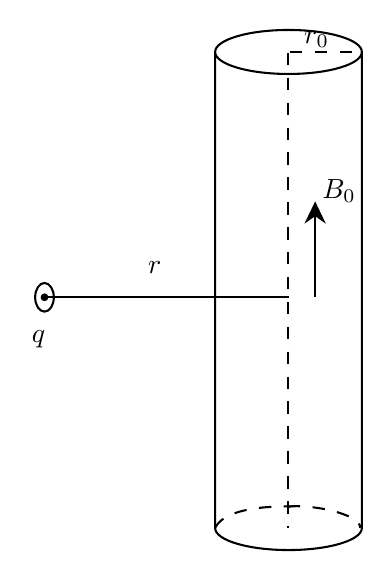
\begin{tikzpicture}[x=0.75pt,y=0.75pt,yscale=-1,xscale=1]
%uncomment if require: \path (0,406); %set diagram left start at 0, and has height of 406

%Curve Lines [id:da5306725541700881] 
\draw  [dash pattern={on 4.5pt off 4.5pt}]  (135.82,293.87) .. controls (141.25,282.46) and (170.97,283.6) .. (172.43,283.6) ;
%Curve Lines [id:da1749338697130831] 
\draw  [dash pattern={on 4.5pt off 4.5pt}]  (170.8,283.62) .. controls (182.05,282.46) and (205.66,287.01) .. (205.77,293.87) ;

%Shape: Can [id:dp11503082838059231] 
\draw   (206.5,64.6) -- (206.5,293.97) .. controls (206.5,299.83) and (190.68,304.58) .. (171.16,304.58) .. controls (151.65,304.58) and (135.82,299.83) .. (135.82,293.97) -- (135.82,64.6) .. controls (135.82,58.75) and (151.65,54) .. (171.16,54) .. controls (190.68,54) and (206.5,58.75) .. (206.5,64.6) .. controls (206.5,70.46) and (190.68,75.2) .. (171.16,75.2) .. controls (151.65,75.2) and (135.82,70.46) .. (135.82,64.6) ;
%Straight Lines [id:da8586041648171499] 
\draw  [dash pattern={on 4.5pt off 4.5pt}]  (171,65) -- (171,294) ;
%Straight Lines [id:da3646486531473332] 
\draw    (184,182.6) -- (184,139.6) ;
\draw [shift={(184,136.6)}, rotate = 450] [fill={rgb, 255:red, 0; green, 0; blue, 0 }  ][line width=0.08]  [draw opacity=0] (10.72,-5.15) -- (0,0) -- (10.72,5.15) -- (7.12,0) -- cycle    ;
%Straight Lines [id:da4387617068242238] 
\draw    (53.6,182.8) -- (171.4,182.8) ;
\draw [shift={(53.6,182.8)}, rotate = 0] [color={rgb, 255:red, 0; green, 0; blue, 0 }  ][fill={rgb, 255:red, 0; green, 0; blue, 0 }  ][line width=0.75]      (0, 0) circle [x radius= 1.34, y radius= 1.34]   ;
%Shape: Ellipse [id:dp878162837478867] 
\draw   (49.1,182.8) .. controls (49.1,178.99) and (51.11,175.9) .. (53.6,175.9) .. controls (56.09,175.9) and (58.1,178.99) .. (58.1,182.8) .. controls (58.1,186.61) and (56.09,189.7) .. (53.6,189.7) .. controls (51.11,189.7) and (49.1,186.61) .. (49.1,182.8) -- cycle ;
%Straight Lines [id:da11815077747906666] 
\draw  [dash pattern={on 4.5pt off 4.5pt}]  (171.9,64.6) -- (206.5,64.6) ;


% Text Node
\draw (186,124.6) node [anchor=north west][inner sep=0.75pt]    {$B_{0}$};
% Text Node
\draw (102,164) node [anchor=north west][inner sep=0.75pt]    {$r$};
% Text Node
\draw (46,197.2) node [anchor=north west][inner sep=0.75pt]    {$q$};
% Text Node
\draw (177.16,53.4) node [anchor=north west][inner sep=0.75pt]    {$r_{0}$};


\end{tikzpicture}
\end{center}

\end{vd}
\begin{loigiai}
Gọi từ trường bên trong ống dây là $B_0$, khi từ trường biến thiên theo thời gian sẽ sinh ra một điện trường xoáy, điện trường xoáy, điện trường xoáy này tác động lên điện tích làm điện tích dịch chuyển. Ta thấy thì vận tốc của điện tích càng lớn thì bán kính quỹ đạo nó sẽ càng nhỏ, nhưng để bán kính quỹ đạo điện tích không vào được hình trụ bên trong thì phải đảm bảo lực Lorentz phải cân bằng với lực quán tính li tâm của điện tích trong hệ quy chiếu quay.\\
Từ thông qua một mặt diện tích $\pi r^2 (r>r_0):$
$$\Phi = \pi (r^2-r_0^2)\cdot \alpha t + B_0\pi r_0^2.$$
Phương trình Maxwell:
\begin{align*}
\dfrac{\mathrm{d}\Phi}{\mathrm{d}t}&=E\cdot2\pi r\\
\Rightarrow E&=\dfrac{(r^2-r_0^2)}{2r}\alpha+\dfrac{\mathrm{d}B_0}{\mathrm{d}t}\cdot\dfrac{r_0^2}{2r}.
\end{align*}
Ta có: $qE=m\dfrac{\mathrm{d}v}{\mathrm{d}t}$,
$$\dfrac{mv^2}{r}=qvB\Rightarrow\dfrac{mv}{r}=q\alpha t$$
Để bán kính không đổi, ta lấy vi phân hai vế với r là hằng số:
$$\dfrac{m\mathrm{d}v}{r}=q\alpha\mathrm{d}t\Rightarrow\dfrac{m\mathrm{d}v}{\mathrm{d}t}=q\alpha r.$$
Từ hai phương trình trên ta rút ra được:
$$E=\alpha r \Rightarrow \dfrac{(r^2-r_0^2)}{2r}\alpha+\dfrac{\mathrm{d}B_0}{\mathrm{d}t}\cdot\dfrac{r_0^2}{2r}=\alpha r.$$
Nhân $2rdt$ lên cả hai vế ta thu được:
$$(r^2-r_0^2)\mathrm{d}B+r_0^2\cdot\mathrm{d}B_0=2r^2\mathrm{d}B.$$
Sau khi chuyển vế ta thu lại được phương trình:
\begin{align*}
    (r^2+r_0^2)\mathrm{d}B&=r_0^2\mathrm{d}B_0 \tag{*}\\
\Rightarrow r^2&=\dfrac{\mathrm{d}B_0}{\mathrm{d}B}r_0^2-r_0^2 \ge r_0^2 \\ \Rightarrow \mathrm{d}B_0 &\ge 2\mathrm{d}B. 
\end{align*}

Thực chất phương trình trên ta chỉ cần quan tâm đến độ biến thiên từ trường, nên giả sử bên trong ống ban đầu có từ trường bằng bao nhiêu không quan trọng, ta chỉ cần biết độ biến thiên của nó bằng bao nhiêu, vì thế ta hoàn toàn có thể chọn ban đầu từ trường bên trong ống bằng $0$.
Vì vậy biểu thức cuối cùng là $B_0 \ge 2B=2\alpha t.$
\end{loigiai}



\begin{vd}[Phanh lại]%câu 1
%USAPhO 2021
Một sợi dây điện dài vô hạn có mật độ điện dài $-\lambda$ nằm dọc theo trục $z$.
Một vỏ trụ cách điện dài vô hạn có bán kính $a$, đồng trục với sợi dây và có thể quay tự do xung quanh trục $z$. Vỏ trụ có moment quán tính trên một đơn vị chiều dài là $I$. Điện tích phân bố đều trên vỏ với mật độ điện tích $\dfrac{\lambda}{2\pi a}$.\\
Hệ được đặt trong từ trường ngoài $B_0\hat{z}$, và ban đầu ở trạng thái nghỉ. Lúc $t=0$, từ trường ngoài giảm chậm về $0$ trong thời gian $T\gg a/c$, trong đó $c$ là tốc độ ánh sáng trong chân không.\\
\begin{center}
    

\tikzset{every picture/.style={line width=0.75pt}} %set default line width to 0.75pt        

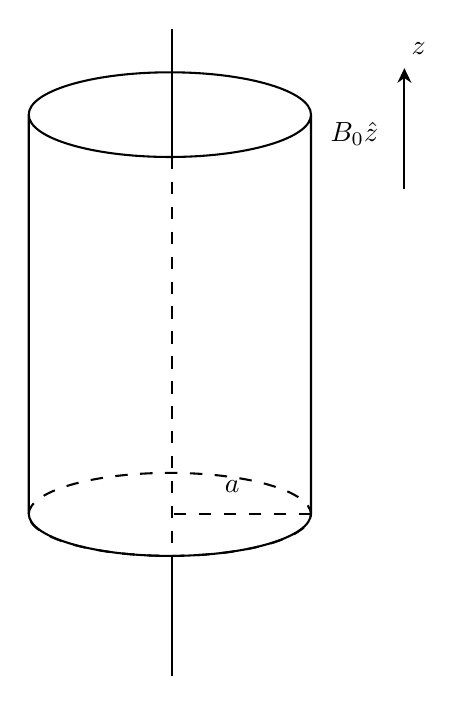
\begin{tikzpicture}[x=0.75pt,y=0.75pt,yscale=-1,xscale=1]
%uncomment if require: \path (0,477); %set diagram left start at 0, and has height of 477

%Shape: Can [id:dp9757468559324121] 
\draw   (359,90.4) -- (359,282.6) .. controls (359,293.87) and (328.56,303) .. (291,303) .. controls (253.44,303) and (223,293.87) .. (223,282.6) -- (223,90.4) .. controls (223,79.13) and (253.44,70) .. (291,70) .. controls (328.56,70) and (359,79.13) .. (359,90.4) .. controls (359,101.67) and (328.56,110.8) .. (291,110.8) .. controls (253.44,110.8) and (223,101.67) .. (223,90.4) ;
%Straight Lines [id:da03285184355277471] 
\draw  [dash pattern={on 4.5pt off 4.5pt}]  (359,282.6) -- (290,282.6) ;
%Shape: Ellipse [id:dp592202237435262] 
\draw  [dash pattern={on 4.5pt off 4.5pt}] (223,283) .. controls (223,271.95) and (253.44,263) .. (291,263) .. controls (328.56,263) and (359,271.95) .. (359,283) .. controls (359,294.05) and (328.56,303) .. (291,303) .. controls (253.44,303) and (223,294.05) .. (223,283) -- cycle ;
%Straight Lines [id:da613160019210224] 
\draw  [dash pattern={on 4.5pt off 4.5pt}]  (292,110.8) -- (292,303) ;
%Straight Lines [id:da5614719570200859] 
\draw    (292,303) -- (292,361) ;
%Straight Lines [id:da3527209195014165] 
\draw    (292,49) -- (292,110.8) ;
%Straight Lines [id:da7119932129755033] 
\draw    (404,126) -- (404,71) ;
\draw [shift={(404,68)}, rotate = 450] [fill={rgb, 255:red, 0; green, 0; blue, 0 }  ][line width=0.08]  [draw opacity=0] (7.14,-3.43) -- (0,0) -- (7.14,3.43) -- (4.74,0) -- cycle    ;

% Text Node
\draw (406,54.4) node [anchor=north west][inner sep=0.75pt]    {$z$};
% Text Node
\draw (367,92.4) node [anchor=north west][inner sep=0.75pt]    {$B_{0}\hat{z}$};
% Text Node
\draw (316,265.4) node [anchor=north west][inner sep=0.75pt]    {$a$};


\end{tikzpicture}

\end{center}
\begin{enumerate} [1)]
    \item Tìm biểu thức vận tốc góc $\omega$ cuối cùng của vỏ trụ, biểu diễn biểu thức theo các dữ kiện đã cho và các hằng số khác.
    \item Bạn có thể ngạc nhiên rằng biểu thức bạn tìm được ở trên không bằng $0$! Tuy nhiên, trường điện từ cũng có moment động lượng. Tương tự như định nghĩa moment động lượng "thông thường", mật độ moment động lượng (trên một đơn vị thể tích) ở khoảng cách $r$ so với trục quay là:
    $$\ot{L\tron{r}}=\ot{r}\times \ot{P\tron{r}}.$$
    $\ot{P\tron{r}}$ là một vector tương tự với động lượng, cho bởi công thức:
    $$\ot{P\tron{r}}=\alpha\cdot\tron{\ot{E\tron{r}}\times \ot{B\tron{r}}},$$
    trong đó $\alpha$ là một hằng số tỷ lệ. Tìm biểu thức của $\alpha$ theo các biến đã cho và các hằng số cơ bản khác.
\end{enumerate}
\end{vd}


\begin{loigiai}

\begin{enumerate}[1)]
    \item Theo định luật Faraday, xuất hiện điện trường cảm ứng bên trong vỏ trụ ở khoảng cách $r$ so với dây dẫn:
    \begin{align*}
        \oint \ot{E}_{\text {xoáy }} \cdot \dd \ot{\ell} &=-\dfrac{\dd \Phi_{B}}{\dd t} \\
        E_{\text {xoáy }}(r) &=-\dfrac{r}{2} \dfrac{\dd B}{\dd t}.
    \end{align*}
   Điện trường cảm ứng này tác động một moment lực lên vỏ trụ, làm vỏ trụ quay:
   $$ \begin{aligned} 
   \tau &=2 \pi a \cdot \dfrac{\lambda}{2 \pi a} \cdot E_{\text {xoáy }}(a) \cdot a=I \cdot \dfrac{\dd \omega}{\dd t} \\
   & \Rightarrow \dfrac{\dd \omega}{\dd t}=-\dfrac{\lambda a^{2}}{2 I} \cdot \dfrac{\dd B}{\dd t}.
   \end{aligned}$$
   Tích phân hai vế với lưu ý rằng $\omega\tron{t=0}=0$, ta có:
   \[\omega\tron{T}=-\dfrac{\lambda a^2}{2I}\tron{B\tron{T}-B_0}.\tag{1}\label{ng1}\]
   Điều quan trọng ta cần lưu ý đó là $B\tron{T}\ne 0$. Kể cả khi từ trường ngoài giảm về không, vỏ trụ tích điện quay sẽ làm sinh ra từ trường. Sử dụng định luật Ampere, ta có thể tìm được cảm ứng từ ở thời điểm $t=T$:
   $$\oint \ot{B}_{\text {xoáy }} \cdot \dd \ot{\ell} =\mu_0 I_{\text{bị quấn}},$$
   trong đó
   \begin{align*}
       I_{\text{bị quấn}}&=\dfrac{\lambda}{2\pi a}\cdot\omega\tron{T}\cdot a,\\
       \Rightarrow B\tron{T}&=\mu_0\dfrac{\lambda}{4\pi^2a}\omega\tron{T}.\tag{2}\label{ng2}
   \end{align*}

   Kết hợp hai phương trình \ref{ng1} và \ref{ng2} ta được:
   $$ \omega(T)=\dfrac{\dfrac{\lambda a^{2}}{2 I} B_{0}}{1+\mu_{0} \dfrac{\lambda^{2} a}{8 \pi I}} .$$
   \item Điện trường bên trong vỏ trụ là $\ot{E}\tron{r}=-\dfrac{\lambda}{2\pi\varepsilon_0r}\hat{r}$ hướng vào trong. Từ trường là $B\tron{t}\hat{z}$. Do đó
   $$\ot{P}\tron{r}=\alpha\dfrac{\lambda\tron{t}}{2\pi\varepsilon_0r}\hat{\theta}.$$
   Mật độ moment động lượng (trong một đơn vị thể tích) khi đó:
   $$\ot{L}\tron{r}=\alpha\dfrac{\lambda}{2\pi\varepsilon_0}\hat{z}.$$
   Mật độ moment động lượng (trên một đơn vị chiều dài) khi đó:
   $$\mathcal{L}=-\dfrac{\alpha\lambda B\tron{t}a^2}{2}\hat{z}.$$
   So sánh với phương trình \ref{ng1} ta được $\alpha=\varepsilon_0$.
\end{enumerate}
\end{loigiai}


\begin{vd}[Hãm đơn cực từ]%câu 11
%USAPhO 2012
Với bài này, giả sử tồn tại một hạt giả thuyết được biết đến như một đơn cực từ. Một hạt như vậy sẽ có ``điện tích từ'' $q_m$, và tương tự với một hạt mang điện sẽ tạo ra một từ trường hướng tâm có độ lớn:
$$B=\dfrac{\mu_0}{4\pi}\dfrac{q_m}{r^2},$$
và chịu một lực tác dụng (trong trường hợp không có điện trường)
$$F=q_m B.$$
Một đơn cực từ có khối lượng m và điện tích từ $q_m$ bị hạn chế chỉ chuyển động máng hình chữ U thẳng đứng, không có từ trường, cách điện, không ma sát. Ở đáy của máng có một vòng dây điện với bán kính $b$ nhỏ hơn rất nhiều so với bề rộng của máng hình chữ U. Do đó, đoạn máng gần vòng dây có thể coi là một đường thẳng. Dây tạo thành vòng dây có bán kính $a\ll b$ và có điện trở suất $\rho$. Đơn cực từ được thả tự do từ độ cao $H$ so với đáy của máng.\\
Bỏ qua độ tự cảm của vòng dây, và giả sử rằng đơn cực từ đi qua vòng dây nhiều lần trước khi dừng lại. 
\begin{enumerate}[1)]
    \item Giả sử đơn cực từ cách tâm vòng dây một khoảng $x$. Hãy tìm từ thông $\Phi_B$ qua vòng dây.
    \item Giả sử rằng ngoài ra đơn cực từ còn chuyển động với vận tốc $v$. Suất điện động $\mathcal{E}$ trong vòng dây là bao nhiêu? 
    \item Tìm độ biến thiên tốc độ $\Delta v$ của đơn cực từ sau mỗi lần đi qua vòng.
    \item Đơn cực từ đi qua vòng dây bao nhiêu lần trước khi dừng lại?
    \item \textbf{Phương pháp thay thế}: Ngoài ra, bạn có thể tìm được đáp án của các phần trên bằng cách sử dụng một hằng số nhân không thứ nguyên (như là $\dfrac{2}{3}$ hoặc $\pi ^2$). Nếu như bạn sử dụng cách thay thế này, bạn vẫn có thể đạt được $60\%$ số điểm của mỗi phần.
\end{enumerate}
Bạn có thể sử dụng các tích phân sau:
$$
\int_{-\infty}^{\infty} \dfrac{1}{\left(1+u^{2}\right)^{3}} \dd u=\dfrac{3 \pi}{8}\quad \text{hoặc}\quad 
\int_{0}^{\pi} \sin ^{4} \theta \dd \theta=\dfrac{3 \pi}{8}.
$$
\end{vd}
\begin{loigiai}
\begin{enumerate}[1)]
    \item Cách tính trực tiếp nhất là tính từ thông xuyên qua một mặt phẳng hình tròn giới hạn bởi vòng. Tuy nhiên, theo định luật Guass thì từ thông sẽ không đổi nếu ta thay đổi hình dạng của mặt phẳng, miễn là ta giữ nguyên đường biên của nó và không động vào đơn cực. Cách dễ nhất là sử dụng mặt có dạng là một phần của hình cầu với bán kính $r=\sqrt{b^2+x^2}$ với tâm trùng với vị trí của đơn cực từ. Sử dụng hệ tọa độ cầu, với $\theta$ là góc hợp với trục $x$ và $\phi$ là góc phương vị. Vòng lặp ở vị trí $\theta_0=tan^{-1}\tron{b/x}$, do đó:
    $$
\Phi_{B}=\dfrac{\mu_{0}}{4 \pi} \frac{q_{m}}{r^{2}} \int_{0}^{2 \pi} \dd \phi \int_{0}^{\theta_{0}} r^{2} \sin \theta \dd \theta=\dfrac{\mu_{0} q_{m}}{2}\left(1-\cos \left(\theta_{0}\right)\right).
$$
Chúng ta có thể dễ dàng kiểm chứng điều này bằng các trường hợp giới hạn: với $x$ nhỏ ta có $\mu_0q_m/2$, tức là một nửa thông lượng, trong khi đó với $x$ lớn thì tổng thông lượng bằng không.
Điều này có thể được chấp nhận, tuy nhiên ta cũng có thể viết nó một cách rõ ràng là một hàm của $x$. Bằng cách vẽ một tam giác vuông, ta có:
$$\sin \theta_0=\dfrac{b}{r}, \text{     }\cos\theta_0=\dfrac{x}{r},$$
dẫn tới:
$$\Phi_B=\dfrac{\mu_0q_m}{2}\tron{1-\dfrac{x}{\sqrt{b^2+x^2}}}.$$
Chúng ta sẽ sử dụng biến $\theta_0$ cho các phần sau và loại bỏ chỉ số dưới.
\item Vì $\mathcal{E}=-\dd \Phi_B/\dd t$, vi phân cả hai vế của phương trình trên ta được:
$$\mathcal{E}=\dfrac{\mu_0q_mv}{2}\dfrac{b^2}{\tron{b^2+x^2}^{3/2}}=\dfrac{mu_0q_mv}{2b}\sin^3\theta,$$
trong đó chúng tôi có sử dụng quy tắc chuỗi (chain rule), với $v\dd x/\dd t$. Cả hai dạng đều được chấp nhận.
\item Xét lực do từ trường sinh ra bởi dòng điện $I$ của vòng dây tác dụng lên đơn cực. Sử dụng định luật Biot-Savart:
$$\ot{B}=\dfrac{\mu_0 I}{4\pi}\int \dfrac{\dd \ot{s}\times \ot{r}}{r^3},$$
trong đó $\ot{r}$ là vector từ đơn cực tới một điểm trên vành, $\dd \ot{s}$ dọc theo vòng và $r=\sqrt{b^2+x^2}$ như trước. Vì $\dd \ot{s}\times \ot{r}=r\sin\theta\dd s$, tích phân cho ta:
$$B=\dfrac{\mu_0I}{4\pi}\dfrac{2\pi b \sin \theta}{r^2}=\dfrac{\mu_0 I}{2b}\sin^3\theta.$$
Lực tác dụng lên đơn cực từ là $F=q_m B$, do đó gia tốc là:
$$a=\dfrac{q_m B}{m}.$$
Cường độ dòng điện $I$ liên hệ với $\mathcal{E}$ theo định luật Ohm, $\mathcal{E}=IR$, trong đó ta sẽ tính $R$ sau. Khi đó:
$$a=\dfrac{\mu_0^2q_m^2v}{4b^2mR}\sin^6\theta.$$
Độ biến thiên vận tốc sau một lần:
$$
\Delta v=\int a \dd t \approx \dfrac{1}{v} \int_{-\infty}^{\infty} a \dd x=\dfrac{1}{v} \int_{0}^{\pi} a \dfrac{\dd x}{\dd \theta} \dd \theta=-\dfrac{b}{v} \int_{0}^{\pi} \dfrac{a}{\sin ^{2} \theta} \dd \theta,
$$
trong đó ta đã coi $v$ gần như không đổi trong một lần đi và đáy của máng là một đường thẳng dài vô hạn. Thay $a$ vào phương trình và sử dụng công thức tích phân thứ hai được cho ở đề:
$$
\Delta v=-\dfrac{\mu_{0}^{2} q_{m}^{2}}{4 b m R} \int_{0}^{\pi} \sin ^{4} \theta \dd \theta=-\dfrac{3 \pi}{32} \dfrac{\mu_{0}^{2} q_{m}^{2}}{b m R}.
$$
Cuối cùng, ta cần tìm $R$. Vì $a\ll b$, nên vòng có thể coi là một sợi dây hình trụ dài, do đó
$$R=\rho\dfrac{2\pi b}{\pi a^2},$$
và cho kết quả cuối cùng là 
$$\Delta v=-\dfrac{3\pi}{64}\dfrac{\mu_0^2q_m^2a^2}{b^2m\rho}.$$
Chúng ta đã không xem xét dấu một cách kĩ lưỡng, điều quan trọng ở đây chính $\Delta v$ mang dấu âm, tuân theo định luật Lenz.\\
Chúng ta cũng có thể giải bài toán này bằng phương pháp bảo toàn năng lượng, tìm năng lượng tiêu hao sau mỗi lượt đi bằng cách tích phân $P=\mathcal{E}^2/R$ theo thời gian, rồi sau đó liên hệ nó với sự biến thiên động năng của đơn cực: $\Delta K\approx mv\Delta v$.\\
Nếu chúng ta tích phân theo $\dd x$, ta sẽ dùng công thức tích phân đầu tiên được cung cấp ở đề. Các công thức tích phân này không quá khó để biến đổi ra. Công thức đầu liên hệ với công thức thứ hai bởi việc thay thế $u$, đối với công thức thứ hai, lưu ý rằng
$$
\int_{0}^{\pi} \sin ^{4} \theta \dd \theta=\int_{0}^{\pi}\left(\frac{e^{i \theta}-e^{-i \theta}}{2 i}\right)^{4} \dd \theta.
$$
Tất cả các số hạng trong phần mở rộng đều tích phân bằng không, ngoại trừ phần hằng số. Do đó tích phân được:
$$
\dfrac{1}{16}\left(\begin{array}{l}
4 \\
2
\end{array}\right) \int_{0}^{\pi} \dd \theta=\dfrac{3 \pi}{8}.
$$
\item Tốc độ ban đầu là $\sqrt{2gH}$ bằng cách bảo toàn năng lượng, do đó:
$$
N=\dfrac{\sqrt{2 g H}}{\Delta v}=\dfrac{64 \sqrt{2}}{3 \pi} \dfrac{b^{2} m \rho \sqrt{g H}}{\mu_{0}^{2} q_{m}^{2} a^{2}}.
$$
\end{enumerate}
\end{loigiai}


 \begin{vd}[Hạt nảy trong trường điện từ]
%DienTuTruong(1*)
Ở hình bên, một vật liệu tấm tròn được đặt trên mặt phẳng ngang $xOy$ và tâm của vòng tròn nằm ở gốc tọa độ $O$, có một điện trường đều có độ lớn $E$ và hướng âm dọc theo trục $z$ phía trên mặt phẳng $xOy$. Có một từ trường đều độ lớn $B$ dọc theo chiều dương trục $z$ trong vùng hình trụ dọc theo trục $z$ với mặt cắt nằm ngang là tấm vật liệu, bên ngoài vùng hình trụ không có từ trường. Các hạt tích điện dương điện tích $q$, khối lượng $m$ và vận tốc $v$ được phát ra đều theo mọi hướng từ gốc $O$ trong vùng không gian phía trên mặt phẳng $xOy$. Ảnh hưởng của trọng lực lên các hạt là không đáng kể và không xét đến sự tương tác giữa các hạt.
\begin{center}
\tikzset{every picture/.style={line width=0.75pt}} %set default line width to 0.75pt        

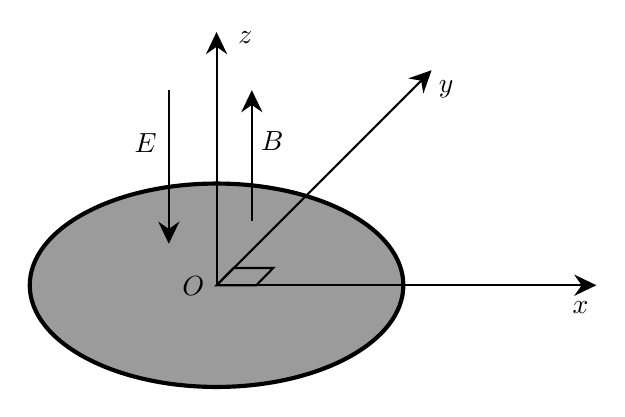
\begin{tikzpicture}[x=0.75pt,y=0.75pt,yscale=-1,xscale=1]
%uncomment if require: \path (0,300); %set diagram left start at 0, and has height of 300

%Shape: Ellipse [id:dp08607047016333724] 
\draw  [fill={rgb, 255:red, 155; green, 155; blue, 155 }  ,fill opacity=1 ][line width=1.5]  (99,154) .. controls (99,126.94) and (139.29,105) .. (189,105) .. controls (238.71,105) and (279,126.94) .. (279,154) .. controls (279,181.06) and (238.71,203) .. (189,203) .. controls (139.29,203) and (99,181.06) .. (99,154) -- cycle ;
%Straight Lines [id:da28751480232453386] 
\draw    (189,154) -- (369,154) ;
\draw [shift={(372,154)}, rotate = 180] [fill={rgb, 255:red, 0; green, 0; blue, 0 }  ][line width=0.08]  [draw opacity=0] (10.72,-5.15) -- (0,0) -- (10.72,5.15) -- (7.12,0) -- cycle    ;
%Straight Lines [id:da44555380527705857] 
\draw    (189,154) -- (189,35) ;
\draw [shift={(189,32)}, rotate = 450] [fill={rgb, 255:red, 0; green, 0; blue, 0 }  ][line width=0.08]  [draw opacity=0] (10.72,-5.15) -- (0,0) -- (10.72,5.15) -- (7.12,0) -- cycle    ;
%Straight Lines [id:da36433558442049985] 
\draw    (166,60) -- (166,131) ;
\draw [shift={(166,134)}, rotate = 270] [fill={rgb, 255:red, 0; green, 0; blue, 0 }  ][line width=0.08]  [draw opacity=0] (10.72,-5.15) -- (0,0) -- (10.72,5.15) -- (7.12,0) -- cycle    ;
%Straight Lines [id:da6562551266395973] 
\draw    (206,123) -- (206,63) ;
\draw [shift={(206,60)}, rotate = 450] [fill={rgb, 255:red, 0; green, 0; blue, 0 }  ][line width=0.08]  [draw opacity=0] (10.72,-5.15) -- (0,0) -- (10.72,5.15) -- (7.12,0) -- cycle    ;
%Shape: Parallelogram [id:dp47425660848965534] 
\draw   (197.2,145.67) -- (216.33,145.67) -- (208.13,154) -- (189,154) -- cycle ;
%Straight Lines [id:da6464703448294327] 
\draw    (189,154) -- (290.47,52.53) ;
\draw [shift={(292.59,50.41)}, rotate = 495] [fill={rgb, 255:red, 0; green, 0; blue, 0 }  ][line width=0.08]  [draw opacity=0] (10.72,-5.15) -- (0,0) -- (10.72,5.15) -- (7.12,0) -- cycle    ;

% Text Node
\draw (148,79.4) node [anchor=north west][inner sep=0.75pt]    {$\ot{E}$};
% Text Node
\draw (209,78.4) node [anchor=north west][inner sep=0.75pt]    {$\ot{B}$};
% Text Node
\draw (359,160.4) node [anchor=north west][inner sep=0.75pt]    {$x$};
% Text Node
\draw (294.59,53.81) node [anchor=north west][inner sep=0.75pt]    {$y$};
% Text Node
\draw (198,30.4) node [anchor=north west][inner sep=0.75pt]    {$z$};
% Text Node
\draw (171,148.4) node [anchor=north west][inner sep=0.75pt]    {$O$};


\end{tikzpicture}
\end{center}
\begin{enumerate}[1)]
    \item Nếu va chạm của các hạt với bề mặt vật liệu là va chạm đàn hồi và tỷ lệ phần trăm của các hạt bị chịu tác động bởi điện trường và từ trường chỉ chuyển động trong vùng hình trụ so với tổng số hạt phát ra là $\eta=50 \%$. Hãy xác định bán kính $R$ của tấm vật liệu.
  \item Khi va chạm với tấm vật liệu, theo phương thẳng hạt bị bật ngược lại và theo phương song song với tấm vật liệu hướng của thành phần nằm ngang của vận tốc được giữ nguyên. Cứ sau mỗi lần va chạm với tấm vật liệu thi động năng của hạt lại giảm $10 \%$.
  \begin{enumerate}[a)]
      \item Tìm giá trị cực đại hình chiếu đường đi của hạt trên mặt phẳng $xOy$ từ lúc phát ra cho đến khi nó va chạm với bề mặt vật liệu lần đầu tiên. \label{iku}
    \item Trong trường hợp tìm được ở câu (\ref{iku}) thì tổng quãng đường đi của hạt trong không gian từ khi phát ra cho tới khi dừng lại trên tấm vật liệu là bao nhiêu?
  \end{enumerate}
    Cho biết: $\di\int \sqrt{1+u^{2}} d u=\dfrac{1}{2} u \sqrt{1+u^{2}}+\dfrac{1}{2} \ln \left(u+\sqrt{1+u^{2}}\right)+C, C$ là hằng số.
    

\end{enumerate}
\end{vd}
\begin{loigiai}
    \begin{enumerate}[1)]
        \item Do bài toán này có đối xứng tròn có tâm tròn trên mặt phẳng $xOy$, nên có thể đặt vận tốc của hạt tích điện dương thành $\left( 0,v\sin \theta ,v\cos \theta  \right)$.\\
        \begin{center}
\tikzset{every picture/.style={line width=0.75pt}} %set default line width to 0.75pt        

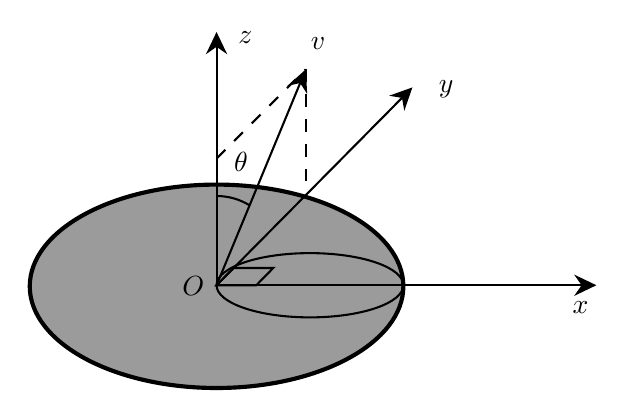
\begin{tikzpicture}[x=0.75pt,y=0.75pt,yscale=-1,xscale=1]
%uncomment if require: \path (0,300); %set diagram left start at 0, and has height of 300

%Shape: Ellipse [id:dp829118797049401] 
\draw  [fill={rgb, 255:red, 155; green, 155; blue, 155 }  ,fill opacity=1 ][line width=1.5]  (99,154.5) .. controls (99,127.44) and (139.29,105.5) .. (189,105.5) .. controls (238.71,105.5) and (279,127.44) .. (279,154.5) .. controls (279,181.56) and (238.71,203.5) .. (189,203.5) .. controls (139.29,203.5) and (99,181.56) .. (99,154.5) -- cycle ;
%Straight Lines [id:da11734275593407639] 
\draw    (189,154) -- (369,154) ;
\draw [shift={(372,154)}, rotate = 180] [fill={rgb, 255:red, 0; green, 0; blue, 0 }  ][line width=0.08]  [draw opacity=0] (10.72,-5.15) -- (0,0) -- (10.72,5.15) -- (7.12,0) -- cycle    ;
%Straight Lines [id:da7284758304058604] 
\draw    (189,154) -- (189,35) ;
\draw [shift={(189,32)}, rotate = 450] [fill={rgb, 255:red, 0; green, 0; blue, 0 }  ][line width=0.08]  [draw opacity=0] (10.72,-5.15) -- (0,0) -- (10.72,5.15) -- (7.12,0) -- cycle    ;
%Shape: Parallelogram [id:dp2735550648263544] 
\draw   (197.2,145.67) -- (216.33,145.67) -- (208.13,154) -- (189,154) -- cycle ;
%Straight Lines [id:da6245275346090199] 
\draw    (189,154) -- (281.23,60.82) ;
\draw [shift={(283.35,58.69)}, rotate = 494.71] [fill={rgb, 255:red, 0; green, 0; blue, 0 }  ][line width=0.08]  [draw opacity=0] (10.72,-5.15) -- (0,0) -- (10.72,5.15) -- (7.12,0) -- cycle    ;
%Shape: Ellipse [id:dp4925988918984876] 
\draw   (189,154) .. controls (189,145.45) and (209.15,138.52) .. (234,138.52) .. controls (258.85,138.52) and (279,145.45) .. (279,154) .. controls (279,162.55) and (258.85,169.48) .. (234,169.48) .. controls (209.15,169.48) and (189,162.55) .. (189,154) -- cycle ;
%Straight Lines [id:da1352953070113686] 
\draw  [dash pattern={on 4.5pt off 4.5pt}]  (189,93) -- (232,50) ;
%Straight Lines [id:da17873733083222787] 
\draw  [dash pattern={on 4.5pt off 4.5pt}]  (232,50) -- (232,111) ;
%Straight Lines [id:da6734265063045801] 
\draw    (189,154) -- (230.85,52.78) ;
\draw [shift={(232,50)}, rotate = 472.46] [fill={rgb, 255:red, 0; green, 0; blue, 0 }  ][line width=0.08]  [draw opacity=0] (10.72,-5.15) -- (0,0) -- (10.72,5.15) -- (7.12,0) -- cycle    ;
%Shape: Arc [id:dp006766106475686207] 
\draw  [draw opacity=0] (188.77,111) .. controls (188.85,111) and (188.92,111) .. (189,111) .. controls (194.82,111) and (200.26,112.63) .. (204.86,115.46) -- (189,140.5) -- cycle ; \draw   (188.77,111) .. controls (188.85,111) and (188.92,111) .. (189,111) .. controls (194.82,111) and (200.26,112.63) .. (204.86,115.46) ;

% Text Node
\draw (359,160.4) node [anchor=north west][inner sep=0.75pt]    {$x$};
% Text Node
\draw (294.59,53.81) node [anchor=north west][inner sep=0.75pt]    {$y$};
% Text Node
\draw (198,30.4) node [anchor=north west][inner sep=0.75pt]    {$z$};
% Text Node
\draw (171,148.4) node [anchor=north west][inner sep=0.75pt]    {$O$};
% Text Node
\draw (196,88.4) node [anchor=north west][inner sep=0.75pt]    {$\theta $};
% Text Node
\draw (233,33.4) node [anchor=north west][inner sep=0.75pt]    {$v$};
\end{tikzpicture}
        \end{center}
        Các hạt bị ràng buộc bởi điện trường và từ trường sẽ tạo ra chuyển động xoắn ốc theo hướng $z$ trong vùng hình trụ với bề mặt vật liệu là đáy (nghĩa là chuyển động tròn đều trong mặt phẳng $xOy$ và chuyển động thẳng biến đổi đều theo hướng $z$).\\
Bán kính của chuyển động tròn đều của hình chiếu của hạt trong mặt phẳng $xOy$ là: 
\[r\left( \theta  \right)=\dfrac{mv\sin \theta }{qB}.\tag{1} \label{y1}\]  
Nếu hạt có thể bị ràng buộc bởi điện trường và từ trường trong một vùng hình trụ thì: \[r\left( \theta  \right)<\dfrac{{{R}_{0}}}{2}. \tag{2} \label{y2}\] 
Coi rằng hướng phát ra của các hạt bị ràng buộc bởi điện trường và từ trường được phân bố đều trong góc khối với trục $z$ là trục đối xứng $\Delta \Omega :0\le \theta \le \Theta ,0\le \phi \le 2\pi $. Bán kính tương ứng với góc khối này là diện tích của một hình cầu có đơn vị chiều dài (giá trị của góc khối $\Delta \Omega$) là:
    \[\Delta \Omega =-2\pi \int\limits_{0}^{\Theta }{\mathrm{d}\cos \theta =2\pi \left( 1-c\text{os}\Theta  \right)}. \tag{3} \label{y3}\] 
Góc khối của các hạt tích điện dương phát ra đồng đều từ gốc $O$ đến mặt phẳng $xOy$ là $2 \pi$. Theo đó các hạt bị ràng buộc bởi điện trường và từ trường chiếm tỷ lệ $\eta$ phần trăm của tổng số hạt phát ra.
\[\eta =\dfrac{\Delta \Omega }{2\pi }=\dfrac{\pi }{2\pi }=50 \%. \tag{4} \label{y4}\] 
Từ (\ref{y3}), (\ref{y4}) suy ra: \[\theta \le \Theta =\dfrac{\pi }{3}. \tag{5} \label{y5}\] 
Thấy rằng các góc $\theta$ phải thỏa mãn điều kiện (\ref{y5}). Từ (\ref{y1}), (\ref{y2}), (\ref{y3}), (\ref{y4}), (\ref{y5}) ta có: \[R=\dfrac{\sqrt{3}mv}{qB}. \tag{6} \label{y6}\]
  \item 
  \begin{enumerate}[a)]
  \item Các hạt tích điện dương tạo ra chuyển động xoắn ốc trong từ trường và vùng điện trường. Thời gian để hạt tạo ra chuyển động tròn trong mặt phẳng chiếu $xOy$ là:
\[T=\dfrac{2\pi r}{v\sin \theta }=\dfrac{2\pi m}{qB}. \tag{7}\] 
Hạt theo hướng $z$ và chọn  thời điểm phát ra của hạt làm mốc không thời gian. Thời điểm trước khi hạt va chạm với bề mặt vật liệu lần đầu tiên là thời gian ${{t}_{1}}\left( \theta  \right)$ được xác định bởi công thức động học:
\[v\cos \theta -a\dfrac{{{t}_{1}}\left( \theta  \right)}{2}=0. \tag{8} \label{y8}\] 
Trong đó: \[a=\dfrac{qE}{m}. \tag{9} \label{y9}\]  Từ (\ref{y8}), (\ref{y9}) ta có: \[{{t}_{1}}\left( \theta  \right)=\dfrac{2mv\cos \theta }{qE}. \tag{10}\] 
Đường đi của hạt trong mặt phẳng $xOy$ để tạo thành chuyển động tròn với độ dài là:
\[d\left( \theta  \right)=2\pi r\left( \theta  \right)=\dfrac{2\pi mv\sin \theta }{qB}. \tag{11}\] 
Quãng đường đi của hạt trên hình chiếu $xOy$ tại thời điểm ${{t}_{1}}\left( \theta  \right)$ là:
\[{{s}_{z=0}}\left( \theta  \right)=\dfrac{{{t}_{1}}\left( \theta  \right)}{T}d\left( \theta  \right)=\dfrac{m{{v}^{2}}}{qE}\sin 2\theta. \tag{12} \] 
Tại $\theta =\dfrac{\pi }{4}$ thì quãng đường đi đạt giá trị lớn nhất:  \[{{s}_{z=0,m\text{ax}}}\left( \theta =\dfrac{\pi }{4} \right)=\dfrac{m{{v}^{2}}}{qE}. \tag{13}\] 
\item Nếu tổng quãng đường di chuyển của hình chiếu của hạt trên mặt phẳng $xOy$ chỉ đạt giá trị cực đại của nó, thì giá trị của $\theta$ được thể hiện trong công thức $\theta =\dfrac{\pi }{4}$. Các hạt được giảm tốc đều theo hướng $z$ và chuyển động tròn đều được thực hiện trên mặt phẳng $xOy$. Chọn thời điểm phát xạ của hạt là mốc thời gian thì vận tốc kết hợp của các hạt tại thời điểm $t$ sau khi phát xạ là:
\[{{v}_{h}}=\sqrt{{{\left( v\sin \dfrac{\pi }{4} \right)}^{2}}+{{\left( vc\text{os}\dfrac{\pi }{4}-at \right)}^{2}}}. \tag{14}\] 
Quãng đường hạt di chuyển cho đến khi va chạm với tấm vật liệu lần thứ $1$ là:
\[{{s}_{1}}=2\int\limits_{0}^{{{t}_{1}}\left( \theta =\dfrac{\pi }{4} \right)/2}{{{v}_{h}}\mathrm{d}t}=\dfrac{m{{v}^{2}}}{qE}\int\limits_{0}^{1}{\sqrt{1+{{u}^{2}}}\mathrm{d}u}. \tag{15}\] 
Áp dụng tích phân thu được: \[{{s}_{1}}=\dfrac{\sqrt{2}+\ln \left( 1+\sqrt{2} \right)}{qE}\dfrac{1}{2}m{{v}^{2}}. \tag{16} \label{y16}\] 
Từ đây có thể thấy, quãng đường đi được phụ thuộc vào động năng sau mỗi lần va chạm. Do đó quãng đường di chuyển được của hạt sau lần va chạm thứ $n$ là: \[{{s}_{n}}={{s}_{1}}\cdot{{k}^{n-1}}. \tag{17}\]
Tổng quãng đường di chuyển được là:
\[{{S}_{t}}={{s}_{1}}+{{s}_{2}}+...+{{s}_{n}}+...={{\left. {{s}_{1}}\left( 1+k+...+{{k}^{n-1}}+... \right) \right|}_{n\to \infty }}={{s}_{1}}\dfrac{1}{1-k}=10{{s}_{1}}. \tag{18} \label{y18}\]
Từ (\ref{y16}), (\ref{y18}) ta có tổng quãng đường đi được là: \[{{S}_{t}}=\left[ \sqrt{2}+\ln \left( 1+\sqrt{2} \right) \right]\dfrac{5m{{v}^{2}}}{qE}. \tag{19}\] 
\end{enumerate}
    \end{enumerate}
    \end{loigiai}
    
    
\begin{vd}[Mô hình lưỡng cực từ]
    Ta xét một mô hình sau cho lưỡng cực từ. Có vài cuộn dây không điện trở được uốn thành hình vuông cạnh $a$. Tại một điểm nào đó trên dây dẫn là nguồn điện nhỏ lí tưởng giữ cho dòng điện $I$ không đổi trong mạch.
    \\ Moment từ $m$ của mạch được cho bởi công thức $m=IA$, với vector $\ot{m}$ chỉ theo phương pháp tuyển của mạch theo quy tắc bàn tay phải, $A$ là diện tích của vòng mạch.
    \begin{enumerate}[1)]
        \item Lưỡng cực được đặt bên trong từ trường đều $\ot{B}$ sao cho góc giữa $\ot{m}$ và $\ot{B}$ là $\theta$. Tìm các góc $\theta_s$ và $\theta_u$ tương ứng với cân bằng bền và không bền. Tính công cần thức hiện để quay lưỡng cực từ $\theta_s$ đế $\theta_u$ theo $m$ và $B$.
    \end{enumerate}
    Chúng ta có thể sử dụng mô hình này để tính toán các đặc tính từ của vật liệu chứa các điện tích chưa ghép đôi có tương tác yếu có thể bỏ qua. Chúng ta hãy xem xét một mẫu vật liệu có $n$ electron chưa ghép đôi trên một đơn vị thể tích, được đặt bên trong từ trường đồng nhất $\ot{B}$. Do spin, mỗi electron chưa ghép đôi hoạt động như một lưỡng cực từ nhỏ. Tuy nhiên, do bản chất lượng tử của electron, hình chiếu của moment từ của nó dọc theo $\ot{B}$ chỉ có thể là $\mu B$ hoặc $-\mu B$ ($\mu B$ được gọi là nam châm Bohr).
    \begin{enumerate}[1)]
    \setcounter{enumi}{1}
        \item Tính M, moment từ trên một đơn vị thể tích của mẫu nếu nhiệt độ của vật liệu là $T$ và từ trường ngoài là $B$.
    \end{enumerate}
\end{vd}

\begin{loigiai}
    \begin{enumerate}[1)]
        \item Khi pháp tuyến vòng dây vuông góc với $\ot{B}$ thì tổng moment lực tác dụng lên vòng dây bằng 0, ứng với 2 giá trị $\theta=0$ và $\theta=\pi$, do đó đây là 2 giá trị của $\theta$ ứng với cân bằng bền và không bền.
        \\Nếu ta quay vòng từ góc $\theta=0$ đến góc $\theta$ nào đó nhưng vẫn giữa cho hai cạnh hình vuông vuông góc với $\ot{B}$, lực Lorentz tác dụng lên hai cạnh này tạo ra một moment lực \[M=-BIa\times a \sin{\theta}=Bm \sin{\theta}\]
        theo chiều giảm của $\theta$.
        \\ Do đối xứng, ta nhận được kết quả tương tự khi lật mặt dưới lên trên.
        \\ Từ đây ta đưa ra kết luận rằng moment quay chỉ phụ thuộc vào $\theta$ và có giá trị ít nhất khi $\theta \to 0$ mà không phụ thuộc vào hướng chính xác của vector pháp tuyển.
        \\ Do đó $\theta_s=0$ và $\theta_u=\pi$.
        \\\\Để làm quay lưỡng cực, ta cần tác dụng một moment lực có độ lớn bằng $M$ và ngược chiều với $M$.
        \\ Công cần thực hiện để quay lượng cực từ $\theta_s$ đến $\theta_u$ là:
        \[A = \int\limits_{{\theta _s}}^{{\theta _u}} { - M{\mathrm{d}}\theta }  =  - \int\limits_0^{2\pi } {{Bm}\sin \theta {\mathrm{d}}\theta }  = 2Bm.\]
        \item Ta biểu diễn số electron (trên một đơn vị thể tích) với phép chiếu moment từ  $+\mu B$ là $n_+$ và những electron có $-\mu B$ là $n_-$. Và tổng của chúng luôn không đổi $n_+ + n_-=n$. Ngoài ra ở trạng thái cân bằng nhiệt, tỷ số của chúng là
        \[\dfrac{n_-}{n_+}=\exp\left({-\dfrac{2\mu_BB }{k_BT}}\right),\]
        với $k_B$ là hằng số Bolzmann.
        \\ Giải hệ phương trình trên, ta tìm được $n_+$ và $n_-$. Tổng moment từ trên một đơn vị thể tích (theo hướng của $\ot{B}$) là $M=\mu_B (n_+ - n_-)$. Tính toán ta tìm được
        \[M=\mu_B N \dfrac{1-\exp\left({\dfrac{2\mu_B B}{k_B T}}\right)}{1 +\exp\left({\dfrac{2\mu_B B}{k_B T}}\right)}=\mu_Bn\tanh\left({\dfrac{\mu_BB}{k_BT}}\right).\]
        
    \end{enumerate}
\end{loigiai}
\begin{vd}[Xuyên qua vùng điện thế] 
    Một hạt mang điện dương được tăng tốc từ điểm gốc bởi của hiệu điện thế $4U$ (trong đó $U> 0$) với một vận tốc nhất định nằm trên mặt phẳng $xy$ dưới góc $30$ độ so với trục $x$ (xem hình vẽ). Hiệu điện thế $V (x, y)  \equiv V (x)$ chỉ phụ thuộc vào toạ độ $x$: nếu $3a <x <4a$ thì $V (x) = U$ và nếu không thì $V (x) = 0$; ngoài lực tĩnh điện không có lực nào khác tác dụng lên hạt và $a> 0$.
    \begin{enumerate}[1)]
        \item Vẽ quỹ đạo của điện tích trên mặt phẳng $xy$ (không cần các số đo hình học hoặc góc).
        \item Nguồn tạo ra các hạt mang điện lúc này là một điốt chân không đồng trục ở gốc tọa độ.
        Do đó các hạt được gia tốc với hiệu điện thế 4U chuyển động đẳng hướng (với số lượng bằng nhau) theo mọi phương của mặt phẳng $xy$; thành phần theo hướng $z$ của vận tốc đối với tất cả các hạt là 0. Phần nào của tất cả các hạt phóng ra đến vùng không gian $x> 4a$?
    \end{enumerate}
    \begin{center}
        

\tikzset{every picture/.style={line width=0.75pt}} %set default line width to 0.75pt        

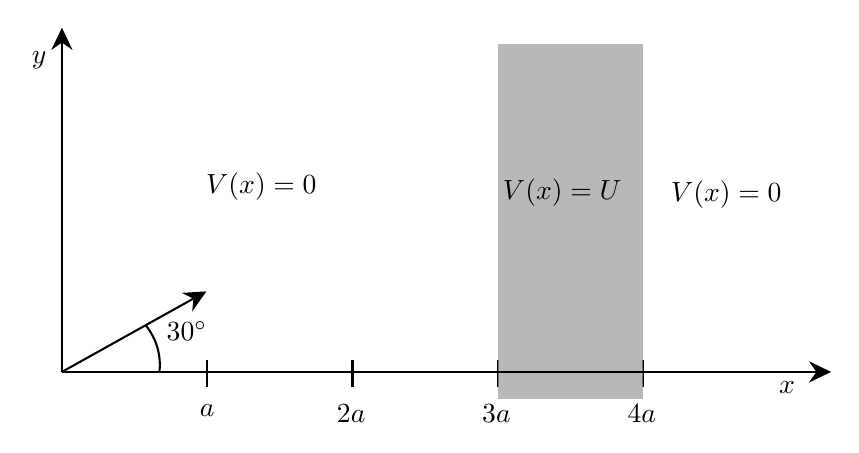
\begin{tikzpicture}[x=0.75pt,y=0.75pt,yscale=-1,xscale=1]
%uncomment if require: \path (0,477); %set diagram left start at 0, and has height of 477

%Straight Lines [id:da7951349378078787] 
\draw    (100,290) -- (100,127.2) ;
\draw [shift={(100,124.2)}, rotate = 450] [fill={rgb, 255:red, 0; green, 0; blue, 0 }  ][line width=0.08]  [draw opacity=0] (10.72,-5.15) -- (0,0) -- (10.72,5.15) -- (7.12,0) -- cycle    ;
%Straight Lines [id:da8964932399673062] 
\draw    (240,284.2) -- (240,297.2) ;
%Straight Lines [id:da6109110947761456] 
\draw    (310,284.2) -- (310,297.2) ;
%Straight Lines [id:da623395669482937] 
\draw    (380,284.2) -- (380,297.2) ;
%Straight Lines [id:da5268431329991505] 
\draw    (170,284.2) -- (170,297.2) ;
%Shape: Rectangle [id:dp042889127368073154] 
\draw  [draw opacity=0][fill={rgb, 255:red, 155; green, 155; blue, 155 }  ,fill opacity=0.71 ] (310,132.2) -- (380,132.2) -- (380,303) -- (310,303) -- cycle ;
%Straight Lines [id:da2161411919818781] 
\draw    (100,290) -- (467.6,290) ;
\draw [shift={(470.6,290)}, rotate = 180] [fill={rgb, 255:red, 0; green, 0; blue, 0 }  ][line width=0.08]  [draw opacity=0] (10.72,-5.15) -- (0,0) -- (10.72,5.15) -- (7.12,0) -- cycle    ;
%Straight Lines [id:da9369052436501601] 
\draw    (100,290) -- (166.98,252.66) ;
\draw [shift={(169.6,251.2)}, rotate = 510.86] [fill={rgb, 255:red, 0; green, 0; blue, 0 }  ][line width=0.08]  [draw opacity=0] (10.72,-5.15) -- (0,0) -- (10.72,5.15) -- (7.12,0) -- cycle    ;
%Shape: Arc [id:dp12073192298003566] 
\draw  [draw opacity=0] (140.63,267.87) .. controls (145.76,274.29) and (147.93,282.45) .. (146.93,290.37) -- (117.17,286.58) -- cycle ; \draw   (140.63,267.87) .. controls (145.76,274.29) and (147.93,282.45) .. (146.93,290.37) ;


% Text Node
\draw (84,134.4) node [anchor=north west][inner sep=0.75pt]    {$y$};
% Text Node
\draw (444,293.4) node [anchor=north west][inner sep=0.75pt]    {$x$};
% Text Node
\draw (168,192.4) node [anchor=north west][inner sep=0.75pt]    {$V( x) =0$};
% Text Node
\draw (311,195.4) node [anchor=north west][inner sep=0.75pt]    {$V( x) =U$};
% Text Node
\draw (392,196.4) node [anchor=north west][inner sep=0.75pt]    {$V( x) =0$};
% Text Node
\draw (165,304.4) node [anchor=north west][inner sep=0.75pt]    {$a$};
% Text Node
\draw (231,304.4) node [anchor=north west][inner sep=0.75pt]    {$2a$};
% Text Node
\draw (301,304.4) node [anchor=north west][inner sep=0.75pt]    {$3a$};
% Text Node
\draw (371,304.4) node [anchor=north west][inner sep=0.75pt]    {$4a$};
% Text Node
\draw (149,264.4) node [anchor=north west][inner sep=0.75pt]    {$30^{\circ }$};


\end{tikzpicture}
    \end{center}
\end{vd}
\begin{loigiai}
    \begin{enumerate}[1)]
        \item Vì điện thế chỉ phụ thuộc vào tọa độ x nên điện trường ở mọi vị trí đều có hướng $x$ và thành phần $y$ của động lượng được bảo toàn.
        Do đó, nếu hạt đi vào vùng có thế năng cao hơn thì chỉ thành phần hướng $x$ của vận tốc giảm và quỹ đạo tương tự như quỹ đạo của tia sáng khi đi sang một môi trường có chiết suất lớn hơn. 
        \item Phản xạ toàn phần xảy ra khi động năng theo phương $x$ theo chiều dương lớn hơn $qU$, góc giữa vận tốc và trục $x$ 
        \[\arccos{\sqrt{\dfrac{qU}{4qU}}}=\dfrac{\pi}{3}.\] 
        Chỉ với những góc nhỏ hơn góc này thì hạt mới có thể đi qua lớp có thế năng lớn hơn và lượng tương đối của các hạt đó đối với tổng các hạt là:
        \[\xi=\dfrac{\pi}{3} \div \pi =\dfrac{1}{3}.\]
    \end{enumerate}
\end{loigiai}


\begin{vd}[Đứt cầu ch...]%câu 13
%USAPhO 2010
Ba phần của bài này có thể trả lời độc lập.
\begin{enumerate}[1.]
    \item Có hai sợi dây dẫn điện dài, song song với nhau, một đầu của mỗi dây được nối với một điện trở $R=0,25~ \mathrm{\Omega}$ và một cầu chì sẽ đứt tức thì nếu có dòng điện $5~ \mathrm{A}$ chạy qua nó. Đầu còn lại của chúng được để tự do. Một thanh dẫn khối lượng $m$ trượt tự do dọc theo dây dưới tác dụng của trọng lực. Hai dây cách nhau $30~ \mathrm{cm}$, thanh bắt đầu chuyển động từ vị trí cách điện trở và cầu chì $10~\mathrm{cm}$. Cả hệ được đặt trong từ trường đều, không đổi $B=1,2\ \mathrm{T}$ như hình vẽ. Điện trở của dây dẫn và của thanh không đáng kể. Khi thanh được thả, nó rơi dưới tác dụng của trọng lực nhưng luôn tiếp xúc với hai dây dẫn.
    \begin{center}
        

\tikzset{every picture/.style={line width=0.75pt}} %set default line width to 0.75pt        

\begin{tikzpicture}[x=0.75pt,y=0.75pt,yscale=-1,xscale=1]
%uncomment if require: \path (0,418); %set diagram left start at 0, and has height of 418

%Straight Lines [id:da17090281026704623] 
\draw    (121,70) -- (121,328) ;
%Straight Lines [id:da5878220563298939] 
\draw    (367,70) -- (367,328) ;
%Shape: Rectangle [id:dp9840410277040863] 
\draw  [fill={rgb, 255:red, 255; green, 255; blue, 255 }  ,fill opacity=1 ] (94,203) -- (397,203) -- (397,229) -- (94,229) -- cycle ;
%Shape: Resistor [id:dp49773719674779127] 
\draw   (121,70) -- (135.4,70) -- (138.6,50) -- (145,90) -- (151.4,50) -- (157.8,90) -- (164.2,50) -- (170.6,90) -- (177,50) -- (183.4,90) -- (186.6,70) -- (201,70) ;
%Straight Lines [id:da33406599682703697] 
\draw    (201,70) -- (230,70) ;
%Shape: Rectangle [id:dp3926228662226221] 
\draw  [fill={rgb, 255:red, 155; green, 155; blue, 155 }  ,fill opacity=1 ] (231,63) -- (308,63) -- (308,77) -- (231,77) -- cycle ;
%Straight Lines [id:da6386859233763178] 
\draw    (309,70) -- (367,70) ;

% Text Node
\draw (134,96.4) node [anchor=north west][inner sep=0.75pt]    {$\text{Điện trở}$};
% Text Node
\draw (244,95.4) node [anchor=north west][inner sep=0.75pt]    {$\text{Cầu chì}$};
% Text Node
\draw (196,170.4) node [anchor=north west][inner sep=0.75pt]    {$\text{Thanh trượt}$};
% Text Node
\draw (122,244.4) node [anchor=north west][inner sep=0.75pt]    {Từ trường có hướng đi vào trang giấy };


\end{tikzpicture}

    \end{center}
    \begin{enumerate}[a)]
        \item Khối lượng của thanh dẫn nhỏ nhất bằng bao nhiêu để làm đứt cầu chì?
        \item Vận tốc của thanh là bao nhiêu sau khi cầu chì bị đứt?
    \end{enumerate}
    \item Một cầu chì được cấu tạo bởi một dây dẫn hình trụ chiều dài $L$ với bán kính là $r\ll L$. Điện trở suất (không phải điện trở!) của cầu chì là $\rho_f$ nhỏ. Giả sử rằng một dòng điện đều $I$ chạy qua cầu chì. Biểu diễn các kết quả của bạn theo $L, r, \rho_f, I$ và các hằng số cơ bản.
    \begin{enumerate}[a)]
        \item Hãy tìm độ lớn và hướng của điện trường trên bề mặt dây cầu chì?
        \item Hãy tìm độ lớn và hướng của từ trường trên bề mặt dây cầu chì?
        \item Vector Poynting $\overrightarrow{S}$ là một đại lượng đo tốc độ năng lượng điện từ qua một đơn vị diện tích, vector cho biết hướng của dòng năng lượng. Với $\ot{S}=\dfrac{1}{\mu_0}\ot{E}\times\ot{B}$, với $\mu_0$ là độ từ thẩm chân không, $\ot{E}$ và $\ot{B}$ lần lượt là vector điện trường và từ trường, hãy tìm độ lớn và hướng của vector Poynting liên quan với dòng điện trong cầu chì.
    \end{enumerate}
    \item Cầu chì sẽ đứt khi nó đạt tới điểm nóng chảy. Chúng ta biết từ vật lí hiện đại rằng một vật thể nóng sẽ bức xạ năng lượng (xấp xỉ) theo định luật vật đen: $P=\sigma A T^4$, trong đó $T$ là nhiệt độ theo nhiệt giai Kelvin, $A$ là diện tích bề mặt, và $\sigma$ là hằng số Stefan-Boltzmann. Nếu $T_f=500\ \mathrm{K}$ là điểm nóng chảy của kim loại làm cầu chì, với điện trở suất $\rho_f=120\ \mathrm{n\Omega\cdot m}$, và $I_f=5\ \mathrm{A}$ là cường độ dòng điện mong muốn khi cầu chì đứt, bán kính $r$ của cầu chì bằng bao nhiêu?
    \end{enumerate}
\end{vd}
\begin{loigiai}
\begin{enumerate}[1]
    \item \begin{enumerate}[a)]
        \item Khi thanh tăng tốc đi xuống, tốc độ biến thiên từ thông tăng, làm tăng suất điện động và do đó dòng điện đi qua cầu chì. Điều này gây ra một lực hướng lên tác dụng vào thanh, do đó nếu như cầu chì không thể bị đứt, thì cuối cùng thanh sẽ đạt vận tốc tới hạn. Do đó, khối lượng nhỏ nhất để làm đứt cầu chì là khối lượng nhỏ nhất để làm đứt cầu chì ngay cả khi thanh đạt vận tốc tới hạn.\\
        Lực lớn nhất có thể tác dụng lên thanh khi cầu chì sắp đứt là:
        $$F=ILB=\tron{5,0\ \mathrm{A}}\tron{0,3\ \mathrm{m}}\tron{1,2\ \mathrm{T}}=1,8\ \mathrm{N}.$$
        Lực này được tác dụng khi thanh có vận tốc tới hạn, do đó độ lớn của nó là $mg$, và:
        $$m=\dfrac{F}{g}=0,17\ \mathrm{kg}.$$
        \item Chúng ta cần phải tìm mối quan hệ giữa lực tác động lên thanh với vận tốc của thanh. Suất điện động trong mạch là:
        $$\mathcal{E}=\dfrac{\dd \Phi_B}{\dd t}=BLv,$$
        trong đó $v$ là vận tốc của thanh, do đó sử dụng định luật Ohm:
        $$F=\dfrac{\mathcal{E}LB}{R}=\dfrac{B^2L^2v}{R}.$$
        Biến đổi để tìm $v$, ta được:
        $$v=\dfrac{FR}{B^2L^2}=\dfrac{\tron{1,8\ \mathrm{N}}\tron{0,25\ \mathrm{\Omega}}}{\tron{1,2\ \mathrm{T}}^2\tron{0,3\ \mathrm{m}}^2}=3,5\ \mathrm{m/s}.$$
    \end{enumerate}
    \item \begin{enumerate}[a)]
        \item Điện trường có nhiệm vụ đẩy dòng điện đi qua cầu chì, nên nó phải có hướng dọc theo cầu chì. Điện trở của cầu chì là:
        $$R_f=\dfrac{\rho_f L}{\pi r^2}.$$
        Theo định nghĩa của điện trường, $E=V_f/L$, trong đó $V_f$ là điện thế trên cầu chì. Theo định luật Ohm ta có:
        $$E=\dfrac{i R_f}{L}=\dfrac{I\rho_f}{\pi r^2}.$$
        \item Theo định luật Ampere, từ trường là:
        $$B=\dfrac{\mu_0 I}{2\pi r},$$
        và nó hướng dọc theo chu vi mạch.
        \item Vì điện trường và từ trường vuông góc nên độ lớn của vector Poynting là:
        $$S=\dfrac{1}{\mu_0}EB=\dfrac{I^2 \rho f}{2\pi^2r^3}.$$
        Dùng quy tắc bàn tay phải, vector Poynting hướng vào dây cầu chì, giải thích vì sao cầu chì nóng lên. Thật vậy, theo phân tích này, tổng công suất cung cấp cho cầu chì là:
        $$P=\tron{2\pi rL}S=\dfrac{I^2\rho_f L}{\pi r^3},$$
        và chính xác bằng $I^2 R_f$.
        \end{enumerate}
        \item Ở trạng thái cân bằng nhiệt, ta có: 
        $$\sigma T^4=\dfrac{I^2\rho_f}{2\pi^2r^3}.$$
        Đặt $T$ thành $T_f$ và $I$ thành $I_f$, giải $r$:
        $$
r=\sqrt[3]{\dfrac{(5 \ \mathrm{A})^{2}\left(120 \times 10^{-9}\ \Omega \cdot \mathrm{m}\right)}{2 \pi^{2}\left(5,67 \times 10^{-8} \ \mathrm{J} /\left(\mathrm{s} \cdot \mathrm{m}^{2} \cdot \mathrm{K}^{4}\right)\right)(500\  \mathrm{K})^{4}}}=0,35\ \mathrm{mm}
$$
\end{enumerate}
\end{loigiai}


\begin{vd}[Nghịch lí Shockley $-$ James] 
%APho 2011 Israel
Trong năm $1905$, Albert Einstein đề xuất thuyết tương đối để giải quyết sự không tương thích giữa cơ học của Newton và thuyết điện từ của Maxwell. Sự hiểu biết đúng đắn của thuyết tương đối dẫn tới việc giải đáp nhiều nghịch lí biểu kiến. Vào thời điểm đó, cuộc tranh luận chủ yếu tập trung vào sự lan truyền của các sóng điện từ.\\
Trong bài toán này, ta giải đáp một nghịch lí khác. Đối với một hệ điện tích khá đơn giản do W. Shockley và R.P. James đề xuất vào năm $1967$, sự hiểu biết và bảo toàn động lượng tuyến tính đòi hỏi phép phân tích tương đối tính cẩn thận. Một điện tích điểm phụ đặt gần một nam châm có độ từ hóa thay đổi, có một lực điện cảm ứng trên điện tích nhưng không có phản ứng biểu kiến trên nam châm. Quá trình có thể đủ chậm để có thể bỏ qua bất kì bức xạ điện từ nào (và bất kì động lượng nào do nó mang theo). Như vậy, nhìn bề ngoài ta có một khẩu pháo không bị giật lùi.\\
Trong phân tích của chúng ta về hệ này, ta sẽ chứng minh rằng trong cơ học tương đối tính, một vật thể kết hợp có thể giữ một động lượng cơ học khác không trong khi nó đứng yên.
\begin{center}
    \bf Sự hiểu biết về xung lực trên điện tích điểm
\end{center}
Xét một mạch điện tròn có bán kính $r$ mang dòng điện $I_1$ và một mạch điện thứ hai có bán kính $R$ lớn hơn $(R\gg r)$ đồng tâm với mạch thứ nhất. Cả hai mạch nằm trong cùng một mặt phẳng.
\begin{enumerate}[1)]
    \item Dòng điện $I_2$ đi qua mạch $2$ (mạch lớn hơn) sinh ra một từ thông $\Phi_{B1}$ qua mạch $1$. Tìm tỉ số $M_{21}=\dfrac{\Phi_{B1}}{I_2}$. Nó được gọi là hệ số hỗ cảm. 
    \item Cho $M_{12}=\dfrac{\Phi_{B2}}{I_1}=M_{21}$, tìm lực điện từ cảm ứng tổng cộng $\varepsilon_2$ trong mạch lớn hơn do sự thay đổi $\Dot{I_1}=\dfrac{\mathrm{d}I_1}{\mathrm{d}t}$ của dòng điện trong mạch nhỏ hơn. Bỏ qua dòng điện trong mạch lớn hơn.\\
    \textbf{Gợi ý:} Lực điện từ cảm ứng bằng tốc độ thay đổi của từ thông qua mạch vòng.
    \item Lực điện từ tìm được trong phần $(2)$ là do thành phần tiếp tuyến của một điện trường cảm ứng. Tìm một biểu thức của điện trường tiếp tuyến $E$ tại bán kính $R$ như là một hàm của tốc độ thay đổi $\Dot{I_1}$ của dòng điện.
    \end{enumerate}
    \begin{center}
        

\tikzset{every picture/.style={line width=0.75pt}} %set default line width to 0.75pt        

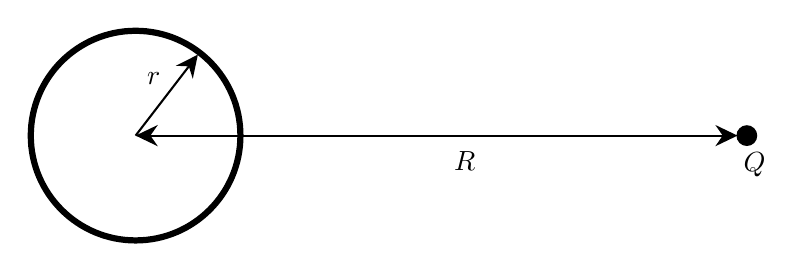
\begin{tikzpicture}[x=0.75pt,y=0.75pt,yscale=-1,xscale=1]
%uncomment if require: \path (0,300); %set diagram left start at 0, and has height of 300

%Shape: Circle [id:dp1365886821011939] 
\draw  [line width=2.25]  (99.5,140.33) .. controls (99.5,112.44) and (122.11,89.83) .. (150,89.83) .. controls (177.89,89.83) and (200.5,112.44) .. (200.5,140.33) .. controls (200.5,168.22) and (177.89,190.83) .. (150,190.83) .. controls (122.11,190.83) and (99.5,168.22) .. (99.5,140.33) -- cycle ;
%Straight Lines [id:da5046555392536871] 
\draw    (153,140.33) -- (437,140.33) ;
\draw [shift={(440,140.33)}, rotate = 180] [fill={rgb, 255:red, 0; green, 0; blue, 0 }  ][line width=0.08]  [draw opacity=0] (10.72,-5.15) -- (0,0) -- (10.72,5.15) -- (7.12,0) -- cycle    ;
\draw [shift={(150,140.33)}, rotate = 0] [fill={rgb, 255:red, 0; green, 0; blue, 0 }  ][line width=0.08]  [draw opacity=0] (10.72,-5.15) -- (0,0) -- (10.72,5.15) -- (7.12,0) -- cycle    ;
%Shape: Circle [id:dp1513516332357332] 
\draw  [fill={rgb, 255:red, 0; green, 0; blue, 0 }  ,fill opacity=1 ] (440,140.33) .. controls (440,137.85) and (442.01,135.83) .. (444.5,135.83) .. controls (446.99,135.83) and (449,137.85) .. (449,140.33) .. controls (449,142.82) and (446.99,144.83) .. (444.5,144.83) .. controls (442.01,144.83) and (440,142.82) .. (440,140.33) -- cycle ;
%Straight Lines [id:da2223599699266785] 
\draw    (150,140.33) -- (178.17,103.71) ;
\draw [shift={(180,101.33)}, rotate = 487.57] [fill={rgb, 255:red, 0; green, 0; blue, 0 }  ][line width=0.08]  [draw opacity=0] (10.72,-5.15) -- (0,0) -- (10.72,5.15) -- (7.12,0) -- cycle    ;

% Text Node
\draw (441.5,147.23) node [anchor=north west][inner sep=0.75pt]    {$Q$};
% Text Node
\draw (302,146.4) node [anchor=north west][inner sep=0.75pt]    {$R$};
% Text Node
\draw (154,108.4) node [anchor=north west][inner sep=0.75pt]    {$r$};


\end{tikzpicture}
    \end{center}
    \begin{center}
        Một mạch điện tròn và một điện tích điểm $Q$.
    \end{center}
    Bây giờ ta loại bỏ mạch điện lớn hơn và để thay thế đặt một điện tích điểm lớn $Q$ tại bán kính $R$ như chỉ ra ở hình trên. Có thể giả thiết rằng điện tích di chuyển rất ít trong các khoảng thời gian có liên quan.
    \begin{enumerate}[1) ]
    \setcounter{enumi}{3}
    \item Tìm xung lực tiếp tuyến toàn phần $\Delta p$ do điện tích điểm nhận được khi dòng điện trong mạch nhỏ thay đổi từ giá trị ban đầu $I_1=1$ đến giá trị cuối cùng $I_1=0$.
\end{enumerate}
\end{vd}
\begin{loigiai}
\begin{enumerate}[1) ]
    \item Tìm tỉ số $M_{21}=\dfrac{\Phi_{B1}}{I_2}$.\\
    Từ trường sinh ra bởi vòng lặp lớn ở tâm của nó là
    \[B=\dfrac{\mu_0I_2}{2R}. \tag{1} \label{apho11sa.1}\]
    Vì $r\ll R$ nên đây là trường qua toàn bộ diện tích của vòng lặp nhỏ. Do đó, từ thông qua vòng lặp nhỏ được cho bởi
    
    \[\phi_{B1}=\pi r^2B=\dfrac{\pi\mu_0r^2I_2}{2R}. \tag{2} \label{apho11sa.2}\]

    Độ hỗ cảm khi đó được tính bởi: 
    
    \[M_{21}=\dfrac{\pi\mu_0r^2}{2R}. \tag{3} \label{apho11sa.3}\]
    
    \item Tìm lực điện từ cảm ứng tổng cộng $\varepsilon_2$ trong mạch lớn hơn do sự thay đổi $\Dot{I_1}=\dfrac{\mathrm{d}I_1}{\mathrm{d}t}$ của dòng điện trong mạch nhỏ hơn.\\
    Vì $M_{21}=M_{12}=M$ nên ta có:

    \[\phi_{B2}=MI_1=\dfrac{\pi\mu_0r^2I_1}{2R}. \tag{4} \label{apho11sa.4}\]
    
    Lấy đạo hàm theo thời gian, nó trở thành
    
    \[\varepsilon_2=\dfrac{\pi\mu_0r^2I_1}{2R}. \tag{5} \label{apho11sa.5}\]
    
    \item Tìm một biểu thức của điện trường tiếp tuyến $E$ tại bán kính $R$ như là một hàm của tốc độ thay đổi $\Dot{I_1}$ của dòng điện.\\
    EMF là công ứng với một đơn vị điện tích trong khi điện trường là lực ứng với một đơn vị điện tích. Vì thế,
    
    \[E=\dfrac{\varepsilon_2}{2\pi R}\dfrac{\mu_0r^2\Dot{I_1}}{4R^2}. \tag{6} \label{apho11sa.6}\]
    
    \item Tìm xung lực tiếp tuyến toàn phần $\Delta p$ do điện tích điểm nhận được khi dòng điện trong mạch nhỏ thay đổi từ giá trị ban đầu $I_1=1$ đến giá trị cuối cùng $I_1=0$.\\
    Điện trường từ phần $(3)$ dẫn đến một lực là:
    
    \[F=EQ=\dfrac{\mu_0r^2Q\Dot{I}}{3R^2}. \tag{7} \label{apho11sa.7}\]
    Khi lấy tích phân theo $\mathrm{d}t$ (và không xét đến dấu), ta thu được
    \[\Delta p=\dfrac{\mu_0r^2IQ}{4R^2}. \tag{8} \label{apho11sa.8}\]
\end{enumerate}
\end{loigiai}


\begin{vd}[Rơi trong từ trường]
Một vòng dây đang lơ lửng trong chân không (không trọng lượng) và mặt phẳng vòng dây song song với mặt phẳng $Oxy$. Trong  $ x <0 $ có một từ trường đều song song với trục $Oz$. Vòng dây cứng hình chữ nhật có chiều rộng $ l=10 \mathrm {~ cm} $ và $ h = 30 \mathrm {~ cm} $. Vòng được làm bằng dây đồng có tiết diện tròn (bán kính $ r = 1,0 \mathrm {~ mm}$). Ở thời điểm  $ t = 0 \mathrm {~ s} $, từ trường ngoài bắt đầu giảm với tốc độ $ 0,025 \mathrm {~ T} / \mathrm {s} $.
\begin{enumerate}[1)]
    \item Tìm gia tốc của vòng ngay sau thời điểm $ t = 0 \mathrm {~ s} $. Cảm ứng từ ban đầu là $ B = 2,0 \mathrm {~T} $ và vòng dây được nhúng $ d = 12 \mathrm {~cm} $ vào trường bên ngoài với cạnh ngắn hơn của nó song song với trục $Oy$.
    \item Ta có thể tăng gia tốc bằng nhiều cách. Kết quả ở ý trước thay đổi thế nào nếu:
    \begin{enumerate}[a)]
        \item Vòng dây được làm bằng dây đồng với độ dày gấp đôi $(r = 2,0 \mathrm {~ mm})$?
        \item Dây ban đầu được quấn ba lần thay vì một (một cuộn dây ngắn gồm ba vòng, các kích thước của hình chữ nhật được giữ nguyên)?
        \item Khối lượng của cuộn dây được giữ không đổi bằng cách dùng một dây có tiết diện bằng nửa tiết diện trước sau đó quấn hai vòng (các kích thước của hình chữ nhật không đổi)? 
        \item Vòng dây được làm bằng một kim loại khác? Kim loại nào cho trong bảng cho kết quả tốt nhất?
        
    \begin{center}
        \begin{tabular}{|l|l|l|}
        \hline Kim loại & Điện trở suất $10^{-8} \mathrm{~m}$ & Khối lượng riêng $10^{3} \mathrm{~kg} / \mathrm{m}^{3}$ \\
        \hline Sắt & $9,71$ & $7,87$ \\
        \hline Đồng & $1,67$ & $8,96$ \\
        \hline Nhôm & $2,65$ & $2,70$ \\
        \hline Liti & $8,55$ & $0,53$ \\
        \hline
        \end{tabular}
        \end{center}
        
        \item Điều gì sẽ xảy ra nếu chúng ta sử dụng dây đồng dày hơn
         để tạo một vòng dây lớn hơn gấp đôi $ (r = 2,0 \mathrm {~ mm}, l=20 \mathrm {~ cm}, h = 60 \mathrm {~ cm}) $ và nhúng nó $ 24 \mathrm {~ cm} $ vào từ trường ngoài?
    \end{enumerate}
\end{enumerate}
\end{vd}
\begin{loigiai}
\begin{enumerate}[1)]
    \item Vòng dây chuyển động do cảm ứng điện từ. Từ trường biến thiên tạo nên suất điện động cảm ứng cho vòng dây. Từ trường ngoài tác động lên vòng dây mang dòng điện.\\
    Suất điện động xuất hiện trong vòng dây:
    $$U=\dfrac{-\dd\Phi}{\dd t}=-A_l\dfrac{\dd B}{\dd t},$$
    với $A_l=ld$.
    Ta có định luật Ohm: $$I=\dfrac{U}{R}$$
    với $$R=\sigma\dfrac{s}{A_\omega}$$
    và $s=2h+2l$ là tổng chiều dài vòng dây, $A_\omega$ là diện tích tiết diện mặt cắt ngang của dây dẫn và $\sigma$ là điện trở suất của đồng. Do đó 
    $$I=\dfrac{U}{R}=\dfrac{A_l\dfrac{\dd B}{\dd t}A_\omega}{\sigma s}=0,0705~\mathrm{A}.$$
    Lực từ có độ lớn $F=IlB$ và gia tốc:
    $$a=\dfrac{F}{m}=\dfrac{A_l\dfrac{\dd B}{\dd t}A_\omega lB}{\sigma s \times \rho A_\omega s}=\dfrac{A_l\dfrac{\dd B}{\dd t} lB}{\sigma \rho s^2}.$$
    Thay số ta tính được
    $$a= 0,627~\mathrm{m/s^2} \approx 0,63~\mathrm{m/s^2}.$$
    (Lực từ tác động lên các hướng khác bằng không hoặc bị triệt tiêu.
    Từ trường do dòng điện tự gây ra không đáng kể so với từ trường ngoài. Suất điện động tự cảm của cuộn dây rất nhỏ so với suất điện động cảm ứng và dòng điện trong vòng dây gần như không đổi, vì tốc độ của cuộn dây rất nhỏ và từ trường bên ngoài biến thiên với tốc độ không đổi. Các lực từ giữa các bộ phận khác nhau là nội lực không gây ảnh hưởng. Tất nhiên, từ trường của bản thân dây dẫn mang dòng điện tác dụng với bản thân dây dẫn một cách đáng kể nhưng trường hợp này luôn xảy ra khi sử dụng $F=BlI$).
    \item \begin{enumerate}[a)]
        \item Dây dày gấp đôi dẫn đến điện trở giảm bốn lần. Từ đó, dòng điện và lực tăng lên bốn lần. Tuy nhiên, khối lượng cũng tăng lên bốn lần nên gia tốc không thay đổi.
        \item Vòng dây được thay thế bằng một cuộn dây có ba vòng, cuộn dây này cho suất điện động lớn gấp ba lần vòng dây trước. Độ dài dây cũng gấp ba lần dẫn đến điện trở tăng ba lần. Do đó dòng điện giữ nguyên độ lớn.
        \\ Dòng điện đi qua tiết diện ba lần dẫn đến lực tăng lên ba lần. Tuy nhiên, sợi dây có khối lượng tăng gấp ba nên gia tốc không thay đổi.
        Theo tính toán:
        $$a=\dfrac{3A_l\dfrac{\dd B}{\dd t}A_\omega 3lB}{\sigma 3s \times \rho A_\omega 3s}=\dfrac{A_l\dfrac{\dd B}{\dd t} lB}{\sigma \rho s^2}.$$
        \item Thay $3$ bằng $2$ vào phép tính trên, ta thu được kết quả không đổi.
        \item Gia tốc lớn nhất được cho bởi vật liệu mà tích của điện trở suất và khối lượng riêng là nhỏ nhất. Nhôm khá tốt, nhưng Liti có vẻ là tốt nhất.
        \item Tăng gấp đôi kích thước, ta được:
        $$a=\dfrac{4A_l\dfrac{\dd B}{\dd t}A_\omega 2lB}{\sigma 2s \times \rho A_\omega 2s}=2\dfrac{A_l\dfrac{\dd B}{\dd t} lB}{\sigma \rho s^2}.$$
        $$a= 1,253 ~\mathrm{m/s^2} \approx 1,25 ~\mathrm{m/s^2}.$$
    \end{enumerate}
\end{enumerate}
\end{loigiai}


\begin{vd}[Electron trôi trong từ trường]
%Prob 2 IPho 1987
\immini{
Trong lòng một buồng hình xuyến có hai thành phần từ trường: Thành phần thứ nhất với cảm ứng từ $\ot{B}$ có độ lớn $B$ không đổi và đường sức từ là những đường tròn đồng tâm $O$, $O$ nằm trên trục đối xứng của buồng hình xuyến; Thành phần thứ hai có cảm ứng từ $\ot{B_1}$ song song với trục buồng xuyến gọi là từ trường lái.\\
Một chùm electron phát ra từ nguồn điểm $P$ đi vào trong từ trường cuộn dây theo phương các đường sức, electron đã được gia tốc bởi hiệu điện thế $V_0$ trước đó. Góc mở của chùm tia $2 \alpha_0$ được xem là rất nhỏ ($2 \alpha_0 \ll 1$). $P$ nằm trên bán kính chính $R$ của hình xuyến.
}
{
\tikzset{every picture/.style={line width=0.75pt}} %set default line width to 0.75pt
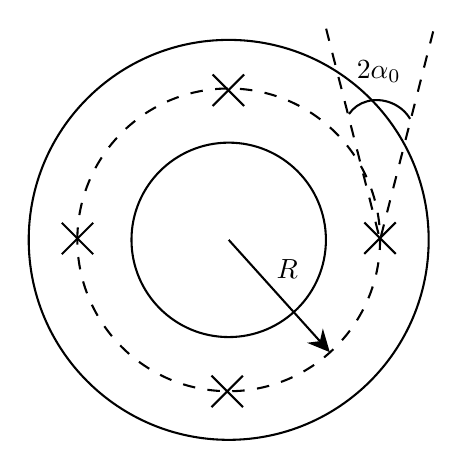
\begin{tikzpicture}[x=0.75pt,y=0.75pt,yscale=-1,xscale=1]
%uncomment if require: \path (0,429); %set diagram left start at 0, and has height of 429

%Shape: Ellipse [id:dp32158213330400987] 
\draw   (201.5,150.98) .. controls (201.5,97.77) and (244.64,54.63) .. (297.85,54.63) .. controls (351.06,54.63) and (394.2,97.77) .. (394.2,150.98) .. controls (394.2,204.2) and (351.06,247.33) .. (297.85,247.33) .. controls (244.64,247.33) and (201.5,204.2) .. (201.5,150.98) -- cycle ;
%Shape: Ellipse [id:dp33436501027685117] 
\draw   (251.01,150.98) .. controls (251.01,125.11) and (271.98,104.14) .. (297.85,104.14) .. controls (323.72,104.14) and (344.69,125.11) .. (344.69,150.98) .. controls (344.69,176.85) and (323.72,197.82) .. (297.85,197.82) .. controls (271.98,197.82) and (251.01,176.85) .. (251.01,150.98) -- cycle ;
%Shape: Ellipse [id:dp7881801386352645] 
\draw  [dash pattern={on 4.5pt off 4.5pt}] (224.92,150.98) .. controls (224.92,110.71) and (257.57,78.05) .. (297.85,78.05) .. controls (338.13,78.05) and (370.78,110.71) .. (370.78,150.98) .. controls (370.78,191.26) and (338.13,223.91) .. (297.85,223.91) .. controls (257.57,223.91) and (224.92,191.26) .. (224.92,150.98) -- cycle ;
\draw   (290.12,71.33) -- (305.27,86.48)(305.27,71.33) -- (290.12,86.48) ;
\draw   (363.2,142.58) -- (378.35,157.73)(378.35,142.58) -- (363.2,157.73) ;
\draw   (289.55,216.42) -- (304.7,231.57)(304.7,216.42) -- (289.55,231.57) ;
\draw   (217.43,142.75) -- (232.58,157.9)(232.58,142.75) -- (217.43,157.9) ;
%Straight Lines [id:da2715309610228023] 
\draw  [dash pattern={on 4.5pt off 4.5pt}]  (344.79,49.25) -- (370.78,150.98) ;
%Straight Lines [id:da4155189959313368] 
\draw  [dash pattern={on 4.5pt off 4.5pt}]  (396.38,50.53) -- (370.78,150.98) ;
%Shape: Arc [id:dp8101916667600975] 
\draw  [draw opacity=0] (355.82,90.37) .. controls (359.81,84.27) and (368.36,81.86) .. (376.2,85.02) .. controls (380.2,86.63) and (383.33,89.41) .. (385.25,92.69) -- (370.51,99.16) -- cycle ; \draw   (355.82,90.37) .. controls (359.81,84.27) and (368.36,81.86) .. (376.2,85.02) .. controls (380.2,86.63) and (383.33,89.41) .. (385.25,92.69) ;
%Straight Lines [id:da6870457753919699] 
\draw    (297.85,150.98) -- (344.55,202.85) ;
\draw [shift={(346.56,205.08)}, rotate = 228] [fill={rgb, 255:red, 0; green, 0; blue, 0 }  ][line width=0.08]  [draw opacity=0] (10.72,-5.15) -- (0,0) -- (10.72,5.15) -- (7.12,0) -- cycle    ;

% Text Node
\draw (358.12,63.06) node [anchor=north west][inner sep=0.75pt]    {$2\alpha _{0}$};
% Text Node
\draw (319.43,158.76) node [anchor=north west][inner sep=0.75pt]    {$R$};
\end{tikzpicture}
}
Bỏ qua tương tác của các electron. Cảm ứng từ $\ot B$ có độ lớn $B$ không đổi.
\begin{enumerate}[1)]
    \item Để giữ chùm electron trong hình xuyến cần phải có một từ trường lái $\ot{B_1}$. Tính $B_1$ cho một electron chuyển động trên quỹ đạo tròn bán kính $R$.
    \item Tính giá trị của $B$ sao cho chùm electron hội tụ ở $4$ điểm cách nhau $\dfrac{\pi}{4}$ như hình vẽ. \\
    \textbf{Lưu ý:} Khi xét quỹ đạo của electron thì có thể bỏ qua độ cong của các đường sức.
    \item Chùm electron không thể được giữ trong hình xuyến mà không có từ trường lái $\ot{B_1}$, nhưng electron vẫn có chuyển động theo phương vuông góc với mặt phẳng của hình xuyến, gọi là sự trôi (drift).
    \begin{enumerate}[a)]
        \item Chứng  tỏ rằng độ lệch của bán kính quỹ đạo electron so với bán kính ban đầu $R$ là hữu hạn.
        \item Xác định chiều của vận tốc trôi.\\
        \textbf{Lưu ý:} Có thể bỏ qua góc mở của chùm electron. Sử dụng định luật bảo toàn năng lượng và moment động lượng.
    \end{enumerate}
Cho các dữ liệu sau:
\[\dfrac{e}{m} = 1,76 \cdot 10^{11} ~\mathrm{C/kg}; \ V_0 = 3~\mathrm{kV}; \ R = 50 ~\mathrm{mm}.\]
\end{enumerate}
\end{vd}
\begin{loigiai}


\begin{enumerate}[1)]
    \item Để electron chuyển động tròn thì từ trường $\ot{B_1}$ phải vuông góc với mặt phẳng hình xuyến và huớng từ sau ra trước hình.\\
    Gọi $v_0$ là vận tốc ban đầu của hạt electron. Áp dụng định luật bảo toàn năng lượng:
    \[eV_0 = \dfrac{mv_0^2}{2}. \tag{1} \label{q.2.1}\]
    Áp dụng định luật II Newton
    \[\ot F = -e \left(\ot{v_0} \times \ot{B_1} \right) = m \ot a \rt ev_0B_1 = m\dfrac{v_0^2}{R}. \tag{2} \label{q.2.2}\]
    Từ (\ref{q.2.1}) và (\ref{q.2.2}), suy ra
    \[B_1 = \dfrac{1}{R} \sqrt{\dfrac{2mV_0}{e}} \approx 3,7 \cdot 10^{-3} ~\mathrm{T}.\]
  
    \item  \immini{Electron chịu tác dụng của hai thành phần lực Lorentz: $\ot{f_1}$ do $\ot{B_1}$ gây ra và $\ot{f}$ do $\ot B$ gây ra nên chuyển động của electron gồm $2$ thành phần: chuyển động tròn bán kính $R$ trên hình xuyến và chuyển động tròn trong mặt phẳng vuông góc với hình xuyến.\\
    Hạt tích điện có vận tốc ban đầu gần song song với từ trường $\ot{B}$ sẽ chuyển động xoắn ốc quanh đường sức. Hình chiếu của quỹ đạo xuống mặt phẳng vuông góc với các đường sức là đường tròn mà bán kính $r$ phụ thuộc vào thành phần $v_r$ của $v_0$ vuông góc với các đường sức.}
    {

\tikzset{every picture/.style={line width=0.75pt}} %set default line width to 0.75pt        

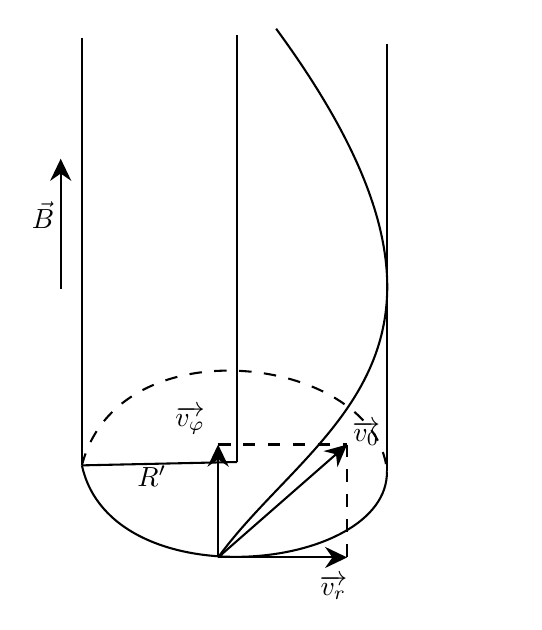
\begin{tikzpicture}[x=0.75pt,y=0.75pt,yscale=-1,xscale=1]
%uncomment if require: \path (0,414); %set diagram left start at 0, and has height of 414

%Curve Lines [id:da5240314896568172] 
\draw  [dash pattern={on 4.5pt off 4.5pt}]  (84.89,264.46) .. controls (102.56,195.31) and (227.29,211.63) .. (231.84,267.29) ;
%Curve Lines [id:da6974779929030936] 
\draw    (84.89,264.46) .. controls (99.02,329.46) and (232.78,315.8) .. (231.84,267.29) ;
%Straight Lines [id:da060845497631258016] 
\draw    (84.89,58.56) -- (84.89,264.46) ;
%Straight Lines [id:da0070370897657010545] 
\draw    (231.84,61.38) -- (231.84,267.29) ;
%Straight Lines [id:da3021302783424833] 
\draw    (159.62,56.94) -- (159.62,262.84) ;
%Straight Lines [id:da25803059907764303] 
\draw    (84.89,264.46) -- (159.62,262.84) ;
%Straight Lines [id:da3153541930273891] 
\draw    (150.51,308.82) -- (209.68,308.82) ;
\draw [shift={(212.68,308.82)}, rotate = 180] [fill={rgb, 255:red, 0; green, 0; blue, 0 }  ][line width=0.08]  [draw opacity=0] (10.72,-5.15) -- (0,0) -- (10.72,5.15) -- (7.12,0) -- cycle    ;
%Straight Lines [id:da2956824367450286] 
\draw    (150.51,257.42) -- (150.51,308.82) ;
\draw [shift={(150.51,254.42)}, rotate = 90] [fill={rgb, 255:red, 0; green, 0; blue, 0 }  ][line width=0.08]  [draw opacity=0] (10.72,-5.15) -- (0,0) -- (10.72,5.15) -- (7.12,0) -- cycle    ;
%Straight Lines [id:da21586844889801204] 
\draw  [dash pattern={on 4.5pt off 4.5pt}]  (212.68,254.42) -- (212.68,308.82) ;
%Straight Lines [id:da772079057267554] 
\draw  [dash pattern={on 4.5pt off 4.5pt}]  (150.51,254.42) -- (212.68,254.42) ;
%Straight Lines [id:da8567133840164769] 
\draw    (74.68,119.73) -- (74.68,179.45) ;
\draw [shift={(74.68,116.73)}, rotate = 90] [fill={rgb, 255:red, 0; green, 0; blue, 0 }  ][line width=0.08]  [draw opacity=0] (10.72,-5.15) -- (0,0) -- (10.72,5.15) -- (7.12,0) -- cycle    ;
%Curve Lines [id:da7817221906021166] 
\draw    (150.51,308.82) .. controls (195.89,246.25) and (292.44,209.51) .. (178.46,54.08) ;
%Straight Lines [id:da4089014962667932] 
\draw    (210.43,256.39) -- (150.51,308.82) ;
\draw [shift={(212.68,254.42)}, rotate = 138.81] [fill={rgb, 255:red, 0; green, 0; blue, 0 }  ][line width=0.08]  [draw opacity=0] (10.72,-5.15) -- (0,0) -- (10.72,5.15) -- (7.12,0) -- cycle    ;

% Text Node
\draw (59.26,136.04) node [anchor=north west][inner sep=0.75pt]    {$\vec{B}$};
% Text Node
\draw (110.11,262.91) node [anchor=north west][inner sep=0.75pt]    {$R'$};
% Text Node
\draw (128.42,234.7) node [anchor=north west][inner sep=0.75pt]    {$\overrightarrow{v_{\varphi }}$};
% Text Node
\draw (197.87,316.18) node [anchor=north west][inner sep=0.75pt]    {$\overrightarrow{v_{r}}$};
% Text Node
\draw (213.76,241.95) node [anchor=north west][inner sep=0.75pt]    {$\overrightarrow{v_{0}}$};
\end{tikzpicture}
}
    Lực Lorentz $\ot f = - e \left(\ot v \times \ot B \right)$ chỉ ảnh hưởng đến thành phần vận tốc vuông góc và đóng vai trò như là một lực hướng tâm. 
    \[m \cdot \dfrac{v_r^2}{R'} = e\cdot v_r \cdot B \rt R' = \dfrac{mv_r}{eB}.\]
    Chu kì quay của hạt trong mặt phẳng vuông góc hình xuyến:
    \[T = \dfrac{2\pi R'}{v_r} = \dfrac{2\pi m}{eB}.\]
    Thành phần $v_\varphi$ song song với các đường sức của $\ot{B}$ không đổi và gần như bằng nhau với mọi electron vì $\alpha_0 \ll 1$.
    \[v_\varphi = v_0 \cos \alpha \approx v_0.\]
    Chu kì chuyển động tròn trên mặt phẳng hình xuyến do $\ot{B_1}$ gây ra là:
    \[T_1 = \dfrac{2\pi R}{v_0} = \dfrac{2\pi m}{eB_1}.\]
    Để hội tụ tại các điểm cách đều nhau $\dfrac{\pi}{4}$ như hình vẽ thì electron thực hiện một chu kì trên quỹ đạo xoắn ốc phải đúng bằng $\dfrac{1}{4}$ chu kì trên đường tròn tâm $O$ bán kính $R$. Suy ra  
    \[T = \dfrac{T_1}{4} \rt \dfrac{2\pi m}{eB} = \dfrac{1}{4} \dfrac{2\pi m}{eB_1} \rt B = 4 B_1.\]
    \[\rt B = \dfrac{4mv_0}{eR} = \dfrac{4}{R} \sqrt{ \dfrac{2mV_0}{e}} \approx 1,48 \cdot 10^{-2}~\mathrm{T}. \]
    \textbf{Lưu ý.} Trên đây chỉ là cách tính gần đúng, ta ngầm coi ${{v}_{z}} \ll {{v}_{r}}$ .
\item 
\textbf{Cách 1.}
   
\begin{center}


\tikzset{every picture/.style={line width=0.75pt}} %set default line width to 0.75pt        

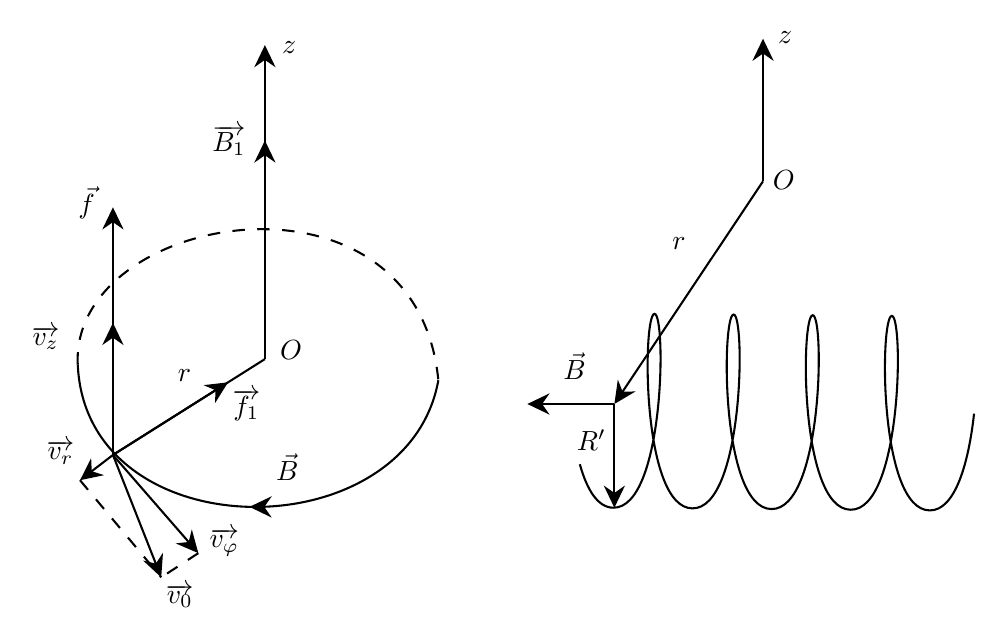
\begin{tikzpicture}[x=0.75pt,y=0.75pt,yscale=-1,xscale=1]
%uncomment if require: \path (0,514); %set diagram left start at 0, and has height of 514

%Curve Lines [id:da7035168393235209] 
\draw  [dash pattern={on 4.5pt off 4.5pt}]  (72.77,266.36) .. controls (69.06,192.88) and (235.85,164.04) .. (246.5,273.94) ;
%Curve Lines [id:da7687825082463489] 
\draw    (246.5,273.94) .. controls (231.65,356.65) and (76.65,356.41) .. (72.77,266.36) ;
\draw [shift={(155.52,334.94)}, rotate = 360.15999999999997] [fill={rgb, 255:red, 0; green, 0; blue, 0 }  ][line width=0.08]  [draw opacity=0] (10.72,-5.15) -- (0,0) -- (10.72,5.15) -- (7.12,0) -- cycle    ;
%Straight Lines [id:da16367591925943126] 
\draw    (162.94,115.46) -- (162.94,263.74) ;
\draw [shift={(162.94,112.46)}, rotate = 90] [fill={rgb, 255:red, 0; green, 0; blue, 0 }  ][line width=0.08]  [draw opacity=0] (10.72,-5.15) -- (0,0) -- (10.72,5.15) -- (7.12,0) -- cycle    ;
%Straight Lines [id:da2631116221321572] 
\draw    (89.72,309.93) -- (128.9,354.97) ;
\draw [shift={(130.87,357.24)}, rotate = 228.98] [fill={rgb, 255:red, 0; green, 0; blue, 0 }  ][line width=0.08]  [draw opacity=0] (10.72,-5.15) -- (0,0) -- (10.72,5.15) -- (7.12,0) -- cycle    ;
%Straight Lines [id:da882066218753899] 
\draw    (89.72,309.93) -- (76.23,320.28) ;
\draw [shift={(73.85,322.1)}, rotate = 322.51] [fill={rgb, 255:red, 0; green, 0; blue, 0 }  ][line width=0.08]  [draw opacity=0] (10.72,-5.15) -- (0,0) -- (10.72,5.15) -- (7.12,0) -- cycle    ;
%Straight Lines [id:da17831705901305472] 
\draw    (89.72,309.93) -- (111.88,366.11) ;
\draw [shift={(112.98,368.9)}, rotate = 248.47] [fill={rgb, 255:red, 0; green, 0; blue, 0 }  ][line width=0.08]  [draw opacity=0] (10.72,-5.15) -- (0,0) -- (10.72,5.15) -- (7.12,0) -- cycle    ;
%Straight Lines [id:da6810161013040124] 
\draw  [dash pattern={on 4.5pt off 4.5pt}]  (73.85,322.1) -- (112.98,368.9) ;
%Straight Lines [id:da28105306605322045] 
\draw  [dash pattern={on 4.5pt off 4.5pt}]  (130.87,357.24) -- (112.98,368.9) ;
%Straight Lines [id:da3106907249369526] 
\draw    (89.72,309.93) -- (162.94,263.74) ;
%Straight Lines [id:da5579940109566166] 
\draw    (89.72,193.62) -- (89.72,309.93) ;
\draw [shift={(89.72,190.62)}, rotate = 90] [fill={rgb, 255:red, 0; green, 0; blue, 0 }  ][line width=0.08]  [draw opacity=0] (10.72,-5.15) -- (0,0) -- (10.72,5.15) -- (7.12,0) -- cycle    ;
%Straight Lines [id:da8908578718782194] 
\draw    (89.72,309.93) -- (142.65,276.54) ;
\draw [shift={(145.19,274.94)}, rotate = 507.75] [fill={rgb, 255:red, 0; green, 0; blue, 0 }  ][line width=0.08]  [draw opacity=0] (10.72,-5.15) -- (0,0) -- (10.72,5.15) -- (7.12,0) -- cycle    ;
%Straight Lines [id:da7820779761356607] 
\draw    (89.72,249.29) -- (89.72,309.93) ;
\draw [shift={(89.72,246.29)}, rotate = 90] [fill={rgb, 255:red, 0; green, 0; blue, 0 }  ][line width=0.08]  [draw opacity=0] (10.72,-5.15) -- (0,0) -- (10.72,5.15) -- (7.12,0) -- cycle    ;
%Straight Lines [id:da06628058185520236] 
\draw    (162.94,161.42) -- (162.94,263.74) ;
\draw [shift={(162.94,158.42)}, rotate = 90] [fill={rgb, 255:red, 0; green, 0; blue, 0 }  ][line width=0.08]  [draw opacity=0] (10.72,-5.15) -- (0,0) -- (10.72,5.15) -- (7.12,0) -- cycle    ;
%Shape: Spring [id:dp7576605960993876] 
\draw   (504.6,290.05) .. controls (502.02,313.42) and (495.62,336.76) .. (483.24,336.65) .. controls (458.46,336.44) and (459.26,242.89) .. (464.98,242.94) .. controls (470.7,242.99) and (469.9,336.54) .. (445.13,336.32) .. controls (420.35,336.11) and (421.15,242.56) .. (426.87,242.61) .. controls (432.59,242.66) and (431.79,336.21) .. (407.01,336) .. controls (382.24,335.79) and (383.04,242.24) .. (388.76,242.28) .. controls (394.47,242.33) and (393.67,335.88) .. (368.9,335.67) .. controls (344.13,335.46) and (344.93,241.91) .. (350.64,241.96) .. controls (356.36,242.01) and (355.56,335.56) .. (330.79,335.35) .. controls (323.23,335.28) and (318.05,326.53) .. (314.67,314.4) ;
%Straight Lines [id:da6895004139447709] 
\draw    (331.31,285.38) -- (331.31,332.35) ;
\draw [shift={(331.31,335.35)}, rotate = 270] [fill={rgb, 255:red, 0; green, 0; blue, 0 }  ][line width=0.08]  [draw opacity=0] (10.72,-5.15) -- (0,0) -- (10.72,5.15) -- (7.12,0) -- cycle    ;
%Straight Lines [id:da45055794815367656] 
\draw    (292.39,285.38) -- (331.31,285.38) ;
\draw [shift={(289.39,285.38)}, rotate = 0] [fill={rgb, 255:red, 0; green, 0; blue, 0 }  ][line width=0.08]  [draw opacity=0] (10.72,-5.15) -- (0,0) -- (10.72,5.15) -- (7.12,0) -- cycle    ;
%Straight Lines [id:da8661821030157217] 
\draw    (402.93,178.08) -- (332.98,282.88) ;
\draw [shift={(331.31,285.38)}, rotate = 303.72] [fill={rgb, 255:red, 0; green, 0; blue, 0 }  ][line width=0.08]  [draw opacity=0] (10.72,-5.15) -- (0,0) -- (10.72,5.15) -- (7.12,0) -- cycle    ;
%Straight Lines [id:da6445710714525845] 
\draw    (402.93,112.39) -- (402.93,178.08) ;
\draw [shift={(402.93,109.39)}, rotate = 90] [fill={rgb, 255:red, 0; green, 0; blue, 0 }  ][line width=0.08]  [draw opacity=0] (10.72,-5.15) -- (0,0) -- (10.72,5.15) -- (7.12,0) -- cycle    ;

% Text Node
\draw (145.85,276.59) node [anchor=north west][inner sep=0.75pt]    {$\overrightarrow{f_{1}}$};
% Text Node
\draw (71.61,179.11) node [anchor=north west][inner sep=0.75pt]    {$\vec{f}$};
% Text Node
\draw (168.75,253.32) node [anchor=north west][inner sep=0.75pt]    {$O$};
% Text Node
\draw (166.86,308.04) node [anchor=north west][inner sep=0.75pt]    {$\vec{B}$};
% Text Node
\draw (136.07,149.63) node [anchor=north west][inner sep=0.75pt]    {$\overrightarrow{B_{1}}$};
% Text Node
\draw (169.7,109.36) node [anchor=north west][inner sep=0.75pt]    {$z$};
% Text Node
\draw (56.3,301.56) node [anchor=north west][inner sep=0.75pt]    {$\overrightarrow{v_{r}}$};
% Text Node
\draw (134.78,343.92) node [anchor=north west][inner sep=0.75pt]    {$\overrightarrow{v_{\varphi }}$};
% Text Node
\draw (113.76,370.56) node [anchor=north west][inner sep=0.75pt]    {$\overrightarrow{v_{0}}$};
% Text Node
\draw (49.14,246.49) node [anchor=north west][inner sep=0.75pt]    {$\overrightarrow{v_{z}}$};
% Text Node
\draw (119.56,267.09) node [anchor=north west][inner sep=0.75pt]    {$r$};
% Text Node
\draw (305.3,258.95) node [anchor=north west][inner sep=0.75pt]    {$\vec{B}$};
% Text Node
\draw (406.23,171.27) node [anchor=north west][inner sep=0.75pt]    {$O$};
% Text Node
\draw (408.69,104.57) node [anchor=north west][inner sep=0.75pt]    {$z$};
% Text Node
\draw (357.71,203.82) node [anchor=north west][inner sep=0.75pt]    {$r$};
% Text Node
\draw (311.76,296.25) node [anchor=north west][inner sep=0.75pt]    {$R'$};
\end{tikzpicture}
\end{center}
\[\overrightarrow{{{f}_{1}}}=-e \tron{\overrightarrow{v}\times \overrightarrow{{{B}_{1}}}} = -e\left| \begin{matrix}
   \overrightarrow{{{e}_{r}}} & \overrightarrow{{{e}_{\varphi }}} & {{\overrightarrow{e}}_{z}}  \\
   {{v}_{r}} & {{v}_{\varphi }} & {{v}_{z}}  \\
   0 & 0 & {{B}_{1}}  \\
\end{matrix} \right|=-e\left({{v}_{\varphi }}{{B}_{1}}\overrightarrow{{{e}_{r}}}+{{v}_{r}}{{B}_{1}}\overrightarrow{{{e}_{\varphi}}}\right) = -e{{B}_{1}}\left({{v}_{\varphi }}\overrightarrow{{{e}_{r}}}+{{v}_{r}}\overrightarrow{{{e}_{\varphi}}}\right).\]
Vì theo câu $1$ thì ${{v}_{r}} \ll {{v}_{\varphi }}$ nên \[\overrightarrow{{{f}_{1}}}\approx -e{{B}_{1}}{{v}_{\varphi }}\overrightarrow{{{e}_{r}}}.\]
Do đó 
\[f_1 = m{{a}_{r}} \rt  e{{v}_{\varphi }}{{B}_{1}} = m\tron{r''+r\varphi'^2} \rt er\varphi '{{B}_{1}} = m\tron{r''+r\varphi'^2}. \tag{3} \label{q.2.3.1}\] 
Ta lại có 
\[\overrightarrow{{{f}_{2}}}=-e \tron{\overrightarrow{v}\times \overrightarrow{B}} = -e\left| \begin{matrix}
   \overrightarrow{{{e}_{r}}} & \overrightarrow{{{e}_{\varphi }}} & {{\overrightarrow{e}}_{z}}  \\
   {{v}_{r}} & {{v}_{\varphi }} & {{v}_{z}}  \\
   0 & B & 0  \\
\end{matrix} \right| = -e \tron{{{v}_{z}}B\overrightarrow{{{e}_{r}}}+{{v}_{r}} B\overrightarrow{{{e}_{z}}}} = -eB\tron{{{v}_{z}}\overrightarrow{{{e}_{r}}}+{{v}_{r}}\overrightarrow{{{e}_{z}}}}.\]
Theo giả thiết câu $2$ thì ${{v}_{z}} \ll {{v}_{r}}$ nên \[\overrightarrow{{{f}_{2}}}\approx -e{{v}_{r}}B\overrightarrow{{{e}_{z}}}\]
\[\rt {{f}_{2}}=mz''\rt {er}'B=mz''.\]
Vì khi $t = 0$ thì $\heva{r &= R \\ z’ &= 0}$ nên 
\[e B (r-R) = mz' \tag{4} \label{q.2.4.1}.\]
Áp dụng định luật bảo toàn moment động lượng:
\[m{{v}_{\varphi }}r = m{{v}_{0}}R \rt {{r}^{2}}\varphi '=R{{v}_{0}}. \tag{5} \label{q.2.5.1}\]
Áp dụng định luật bảo toàn năng lượng
\[\dfrac{m}{2} \left( v_r^2 + v_\varphi^2 + v_z^2\right) = \dfrac{m}{2}v_0^2 \rt v_{r}^{2}+v_{\varphi }^{2}+v_{z}^{2} = v_{0}^{2}.\] 
Hay 
\[r'^2+{{\tron{r\varphi'}}^{2}}+{{\tron{z'}}^{2}} = v_{0}^{2}.\tag{6} \label{q.2.6.1}\]  
Từ (\ref{q.2.4.1}) ta rút $z'=\dfrac{eB}{m}(r-R)$  và từ (\ref{q.2.5.1}) $\varphi '=\dfrac{R{{v}_{0}}}{{{r}^{2}}}$ rồi thay vào (\ref{q.2.6.1}) ta được
\[r{{'}^{2}} + \tron{{r\dfrac{{{v}_{0}}R}{{{r}^{2}}}}}^{2}+ \tron{{\dfrac{eB}{m}(r-R)}}^{2} = v_{0}^{2}.\]
Ta đặt $x = r-R$ thay vào ta được 
\[x{{'}^{2}} + \tron{{\dfrac{{{v}_{0}}R}{x+R}}}^{2} + \tron{{\dfrac{eB}{m}x}}^{2} = v_{0}^{2}.\]
Đạo hàm hai vế theo thời gian:
\[x'x''-\dfrac{{{\tron{{v}_{0}R}}^{2}}}{{{(x+R)}^{3}}}x'+\tron{{\dfrac{eB}{m}}}^{2}xx'=0.\]
\[\rt x''-\dfrac{{{({{v}_{0}}R)}^{2}}}{{{(x+R)}^{3}}} + \tron{{\dfrac{eB}{m}}}^{2}x=0.\]
Vì ${{\alpha }_{0}} \ll 1$  nên $x \ll R$. Do đó ta lấy gần đúng
\[x''-\dfrac{{{({{v}_{0}}R)}^{2}}}{{{R}^{3}}}\tron{1-\dfrac{3x}{R}}+{\tron{\dfrac{eB}{m}}^{2}}x=0.\]
Hay
\[x''+\left( 3{\tron{\dfrac{{{v}_{0}}}{R}}^{2}}+{\tron{\dfrac{eB}{m}}^{2}} \right)x-\dfrac{{{v}_{0}}^{2}}{R} = 0.\]
Đặt ${{\omega }^{2}} =  3{\tron{\dfrac{{{v}_{0}}}{R}}^{2}}+{\tron{\dfrac{eB}{m}}^{2}} $, ta suy ra $x''+{{\omega }^{2}}x-\dfrac{{{v}_{0}}^{2}}{R}=0$
hay
\[\tron{x-\dfrac{{{v}_{0}}^{2}}{R{{\omega }^{2}}}}''+{{\omega }^{2}}\tron{x - \dfrac{{{v}_{0}}^{2}}{R{{\omega }^{2}}}}=0.\]
Vậy 
\[r = x + R = R + \dfrac{{{v}_{0}}^{2}}{R{{\omega }^{2}}}+A\cos (\omega t+\Phi ). \tag{7}\label{q.2.7.1}\]
Mà lúc $t=0$ thì $\heva{r(0) &= R  \\ r'(0) &= 0} 
\rt \heva{   0 &= \dfrac{{{v}_{0}}^{2}}{R{{\omega }^{2}}} + A\cos \Phi \\ 0 &=-\omega A\sin \Phi} 
\rt \heva{\Phi &=\pi   \\ A &= \dfrac{{{v}_{0}}^{2}}{R{{\omega }^{2}}} }$.\\
Thay vào (\ref{q.2.7.1}), ta được
\[r = R + \dfrac{{{v}_{0}}^{2}}{R{{\omega }^{2}}}\left( 1 - \cos\omega t \right). \tag{8}\label{q.2.8.1}\]
\begin{enumerate}[a)]
    \item  Từ (\ref{q.2.8.1}) ta thấy
    \[\heva{{{r}_{\min}} &= R \\ {{r}_{\max}} &= R + 2\dfrac{{{v}_{0}}^{2}}{R{{\omega}^{2}}} = R + \dfrac{2v_{0}^{2}}{R\left( 3{{\tron{\dfrac{{{v}_{0}}}{R}}}^{2}}+{{\tron{\dfrac{eB}{m}}}^{2}} \right)}}.\]
    Vậy độ lệch của bán kính quỹ đạo electron so với bán kính ban đầu $R$ là hữu hạn.
    \item Thay (\ref{q.2.8.1}) vào (\ref{q.2.4.1}) ta được \[{{v}_{z}} = z' = \dfrac{{e}B}{m}(r-R) = \dfrac{{e}B}{m}\dfrac{{{v}_{0}}^{2}}{R{{\omega }^{2}}}\left( 1-\cos \omega t \right)\ge 0. \tag{9} \label{q.2.9.1}\]
Từ (\ref{q.2.9.1}) ta thấy electron luôn trôi theo chiều dương trục $Oz$.
\end{enumerate}

\textbf{Cách 2: Theo đáp án.}\\
Trong từ trường, các đường sức là những đường tròn có tâm nằm trên trục đối xứng (trục $z$) của hình xuyến. Sử dụng hệ tọa độ cực $(r, \varphi, z)$, các đại lượng vector (vận tốc, từ trường, lực Lorentz) cũng sẽ được phân tích thành các thành phần tương ứng.\\
Vì góc mở của chùm tia có thể bị bỏ qua, nên ta chỉ cần xét một electron được bắn vào hình xuyến ở bán kính $R$ với vận tốc $v_0$ gần tiếp tuyến.\\
Trong từ trường tĩnh, động năng của electron được bảo toàn 
\[E = \dfrac{m}{2}v_0^2 = \dfrac{m}{2} \left( v_r^2 + v_\varphi^2 + v_z^2\right).\]
Những điểm đảo của quỹ đạo electron (ở đó bán kính $r$ đạt cực trị) được xác định bởi:
\[v_r = 0.\]
Tại đó 
\[v_0^2 = v_\varphi^2 + v_z^2. \tag{10}\label{q.2.10}\]
Ta có một điểm đảo là 
\[r = R \ (v_\varphi = v_0, v_r = 0, v_z = 0).\]
Để tìm độ lệch cực đại theo bán kính, ta tìm các điểm đảo khác. Ta phải viết $v_\varphi$ và $v_z$ theo bán kính.\\
Lực Lorentz do từ trường $B$ sinh  ra  không có thành phần nào theo phương $\varphi$ song song với nó nên moment động lượng của electron đối với trục $z$ được bảo toàn:
\[mv_\varphi r = mv_0R \rt v_\varphi = v_0 \dfrac{R}{r}. \tag{11}\label{q.2.11}\]
Lực Lorentz có thể có thành phần theo phương $z$
\[{F_z} = {eB} {v_r} = m a_z \rt a_{z} = \dfrac{e}{m} Bv_r. \]
Điều này có nghĩa là (với $B$ không đổi) một biến thiên của $v_z$ liên hệ với một biến thiên của $r$ theo hệ thức:
\[\Delta v_{z} = \dfrac{e}{m} B \Delta r.\]
vì $\Delta r = r - R$ và $\Delta v_{z} = v_{z}$ nên ta có :
\[v_z = \dfrac{e}{m}B (r-R). \tag{12}\label{q.2.12}\]
Thay (\ref{q.2.11}) và (\ref{q.2.12}) vào (\ref{q.2.10}), ta được
\[{v}_{0}^{2}={v}_{0}^{2}\left(\dfrac{{R}}{{r}}\right)^{2}+\left(\dfrac{{e}}{{m}} {B}({r}-{R})\right)^{2}.\]
\[\rt 1 = \left(\dfrac{R}{r}\right)^{2} + A^{2}\left(\dfrac{r }{R} - 1\right)^{2}. \tag{13}\label{q.2.13}\]
Với $A=\dfrac{e}{m}\cdot \dfrac{BR}{v_{0}}$
(\ref{q.2.13}) là phương trình để tìm điểm đảo.
Coi vế phải của (\ref{q.2.13}) là hàm số theo biến $r$:
\[y = f(r) = \left(\dfrac{R}{r}\right)^{2}+A^{2}\left(\dfrac{r}{R} - 1\right)^{2}.\]
\begin{center}
    

\tikzset{every picture/.style={line width=0.75pt}} %set default line width to 0.75pt        

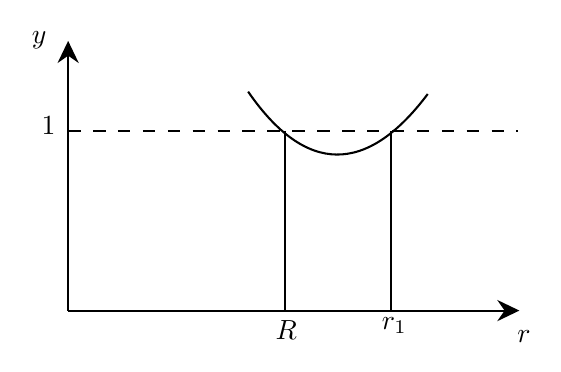
\begin{tikzpicture}[x=0.75pt,y=0.75pt,yscale=-1,xscale=1]
%uncomment if require: \path (0,432); %set diagram left start at 0, and has height of 432

%Straight Lines [id:da5222807838476842] 
\draw    (97.06,101.6) -- (97.06,228.53) ;
\draw [shift={(97.06,98.6)}, rotate = 90] [fill={rgb, 255:red, 0; green, 0; blue, 0 }  ][line width=0.08]  [draw opacity=0] (10.72,-5.15) -- (0,0) -- (10.72,5.15) -- (7.12,0) -- cycle    ;
%Straight Lines [id:da41235855048673375] 
\draw    (97.06,228.53) -- (311.47,228.53) ;
\draw [shift={(314.47,228.53)}, rotate = 180] [fill={rgb, 255:red, 0; green, 0; blue, 0 }  ][line width=0.08]  [draw opacity=0] (10.72,-5.15) -- (0,0) -- (10.72,5.15) -- (7.12,0) -- cycle    ;
%Straight Lines [id:da8265964686331111] 
\draw  [dash pattern={on 4.5pt off 4.5pt}]  (97.06,141.91) -- (313.61,141.91) ;
%Straight Lines [id:da9830243217808909] 
\draw    (201.58,141.8) -- (201.58,228.47) ;
%Straight Lines [id:da08572165924514441] 
\draw    (252.51,142.08) -- (252.51,228.66) ;
%Curve Lines [id:da03506710090141296] 
\draw    (183.77,123.04) .. controls (211.49,163.27) and (240.94,163.27) .. (270.3,124.2) ;

% Text Node
\draw (78.06,92.73) node [anchor=north west][inner sep=0.75pt]    {$y$};
% Text Node
\draw (311.94,236.52) node [anchor=north west][inner sep=0.75pt]    {$r$};
% Text Node
\draw (82.74,133.79) node [anchor=north west][inner sep=0.75pt]    {$1$};
% Text Node
\draw (195.51,232.09) node [anchor=north west][inner sep=0.75pt]    {$R$};
% Text Node
\draw (246.7,230.51) node [anchor=north west][inner sep=0.75pt]    {$r_{1}$};
\end{tikzpicture}
\end{center}
Đồ thị của hàm này có dạng như hình. Ngoài nghiệm $r = R$, phương trình (\ref{q.2.13}) còn có một nghiệm $r = r_1 > R$ nhưng hữu hạn. Vì vậy $r - R$ là hữu hạn. Vì $R \le r \le r_1$, phương trình (\ref{q.2.12}) cho thấy $v_z < 0$, vận tốc trôi theo chiều dương của trục $z$.
\end{enumerate}
\end{loigiai}


\begin{vd}[Làm cong đường thẳng]%câu 12
%bài 2088 Lim 
Một nam châm lưỡng cực với các mặt hình chữ nhật, từ trường $B_0$ và các kích thước đã được chỉ rõ trong các hình $1$ và $2$. Chúng ta đưa vào một hệ trục tọa độ có trục $x$ song song với từ trường và trục $y$, trục $z$ song song với các cạnh của các mặt cực. Hãy chọn mặt phẳng $x=0$ sao cho nó nằm ở giữa khoảng cách các mặt cực. Giả thiết rằng một hạt có điện tích $q$ và động lượng $\ot{P}$ song song với trục $z$ được phóng vào nam châm, đi vào vùng giữa các mặt cực tại một chiều cao $x$ trên mặt phẳng trung tâm $x=0$.
\begin{enumerate}[1)]
    \item Độ lệch góc gần đúng $\theta_y$ là bao nhiêu trong mặt phẳng $yz$ sau khi hạt đi qua nam châm? (Giả thiết $P\gg qBL$)?
    \item Hãy chứng minh rằng độ lệch góc trong mặt phẳng $xz$ sau khi hạt đi qua nam châm được tính gần đúng bằng $\theta_x\approx\theta_y^2 x/L$, với $\theta_y$ là độ lệch tìm thấy trong 1). (Gợi ý: Độ lệch này được sinh ra bởi từ trường rìa tác động lên hạt, khi nó ra khỏi nam châm).
    \item Hiệu ứng tìm được trong 2) hội tụ hay không hội tụ các hạt vào trục?
\begin{center}
    

\tikzset{every picture/.style={line width=0.75pt}} %set default line width to 0.75pt        

\begin{tikzpicture}[x=0.75pt,y=0.75pt,yscale=-1,xscale=1]
%uncomment if require: \path (0,417); %set diagram left start at 0, and has height of 417

%Straight Lines [id:da8637127663714128] 
\draw  [dash pattern={on 4.5pt off 4.5pt}]  (104,227) -- (227,227) ;
%Straight Lines [id:da15932424549463642] 
\draw    (55,227) -- (94,227) ;
\draw [shift={(97,227)}, rotate = 180] [fill={rgb, 255:red, 0; green, 0; blue, 0 }  ][line width=0.08]  [draw opacity=0] (7.14,-3.43) -- (0,0) -- (7.14,3.43) -- (4.74,0) -- cycle    ;
%Straight Lines [id:da4432954559934228] 
\draw    (55,227) -- (55,108) ;
\draw [shift={(55,105)}, rotate = 450] [fill={rgb, 255:red, 0; green, 0; blue, 0 }  ][line width=0.08]  [draw opacity=0] (7.14,-3.43) -- (0,0) -- (7.14,3.43) -- (4.74,0) -- cycle    ;
%Straight Lines [id:da4253436154248016] 
\draw    (100,198) -- (126,198) ;
\draw [shift={(129,198)}, rotate = 180] [fill={rgb, 255:red, 0; green, 0; blue, 0 }  ][line width=0.08]  [draw opacity=0] (7.14,-3.43) -- (0,0) -- (7.14,3.43) -- (4.74,0) -- cycle    ;
\draw [shift={(100,198)}, rotate = 0] [color={rgb, 255:red, 0; green, 0; blue, 0 }  ][fill={rgb, 255:red, 0; green, 0; blue, 0 }  ][line width=0.75]      (0, 0) circle [x radius= 2.01, y radius= 2.01]   ;
%Straight Lines [id:da5931923932152467] 
\draw  [dash pattern={on 4.5pt off 4.5pt}]  (100,198) -- (100,227) ;
%Straight Lines [id:da5668216750179997] 
\draw    (162,257.6) -- (162,201.6) ;
\draw [shift={(162,198.6)}, rotate = 450] [fill={rgb, 255:red, 0; green, 0; blue, 0 }  ][line width=0.08]  [draw opacity=0] (7.14,-3.43) -- (0,0) -- (7.14,3.43) -- (4.74,0) -- cycle    ;
%Straight Lines [id:da7914747612787705] 
\draw    (188.6,257.1) -- (188.6,201.1) ;
\draw [shift={(188.6,198.1)}, rotate = 450] [fill={rgb, 255:red, 0; green, 0; blue, 0 }  ][line width=0.08]  [draw opacity=0] (7.14,-3.43) -- (0,0) -- (7.14,3.43) -- (4.74,0) -- cycle    ;
%Straight Lines [id:da08381806521057644] 
\draw    (215.2,257) -- (215.2,201) ;
\draw [shift={(215.2,198)}, rotate = 450] [fill={rgb, 255:red, 0; green, 0; blue, 0 }  ][line width=0.08]  [draw opacity=0] (7.14,-3.43) -- (0,0) -- (7.14,3.43) -- (4.74,0) -- cycle    ;
%Curve Lines [id:da5900907473583501] 
\draw    (135.8,255.8) .. controls (125.78,236.9) and (128.27,215.86) .. (135.32,200.77) ;
\draw [shift={(136.6,198.2)}, rotate = 477.76] [fill={rgb, 255:red, 0; green, 0; blue, 0 }  ][line width=0.08]  [draw opacity=0] (7.14,-3.43) -- (0,0) -- (7.14,3.43) -- (4.74,0) -- cycle    ;
%Curve Lines [id:da9529440593799141] 
\draw    (240,254.8) .. controls (246.55,240.03) and (244.87,213.89) .. (238.09,200.74) ;
\draw [shift={(236.6,198.2)}, rotate = 416.31] [fill={rgb, 255:red, 0; green, 0; blue, 0 }  ][line width=0.08]  [draw opacity=0] (7.14,-3.43) -- (0,0) -- (7.14,3.43) -- (4.74,0) -- cycle    ;
%Straight Lines [id:da6603859605542026] 
\draw    (135.2,266.8) -- (135.2,313.4) ;
%Straight Lines [id:da871228628163446] 
\draw    (240,266) -- (240,312.6) ;
%Straight Lines [id:da1245911107186386] 
\draw    (135.2,266.8) -- (240,266.8) ;
%Straight Lines [id:da9525014004439876] 
\draw    (203,302.8) -- (237,302.8) ;
\draw [shift={(240,302.8)}, rotate = 180] [fill={rgb, 255:red, 0; green, 0; blue, 0 }  ][line width=0.08]  [draw opacity=0] (7.14,-3.43) -- (0,0) -- (7.14,3.43) -- (4.74,0) -- cycle    ;
%Straight Lines [id:da39707386368649145] 
\draw    (170.4,303.2) -- (138,303.2) ;
\draw [shift={(135,303.2)}, rotate = 360] [fill={rgb, 255:red, 0; green, 0; blue, 0 }  ][line width=0.08]  [draw opacity=0] (7.14,-3.43) -- (0,0) -- (7.14,3.43) -- (4.74,0) -- cycle    ;
%Straight Lines [id:da26699897229317937] 
\draw    (135,137.2) -- (135,182.2) ;
%Straight Lines [id:da8093385246903582] 
\draw    (240.6,137.2) -- (240.6,182.2) ;
%Straight Lines [id:da67876198559254] 
\draw    (135,182.2) -- (207.8,182.2) ;
%Straight Lines [id:da9867586562441406] 
\draw    (232.6,182.2) -- (240.6,182.2) ;
%Straight Lines [id:da30923457978147684] 
\draw    (226.4,197) -- (226.4,226.4) ;
%Straight Lines [id:da2246206105259385] 
\draw    (226.4,197) -- (279,197) ;
%Straight Lines [id:da6675321239462282] 
\draw    (227,227) -- (279.6,227) ;
%Straight Lines [id:da4338106154678849] 
\draw    (278.7,190.9) -- (278.7,201.9) ;
%Straight Lines [id:da18653827662492994] 
\draw    (286.2,190.9) -- (286.2,201.9) ;
%Straight Lines [id:da023473812527841753] 
\draw    (279.2,220.9) -- (279.2,231.9) ;
%Straight Lines [id:da5639286170039737] 
\draw    (286.2,220.9) -- (286.2,231.9) ;
%Straight Lines [id:da8450688146497629] 
\draw    (287.2,197.2) -- (306.2,197.2) ;
%Straight Lines [id:da6993054073770588] 
\draw    (287.4,226.8) -- (306.4,226.8) ;
%Straight Lines [id:da5826344832395913] 
\draw    (306.2,197.2) -- (306.2,226.8) ;
%Straight Lines [id:da7540786571048181] 
\draw    (225.6,197) -- (256.2,197) ;
\draw [shift={(258.2,197)}, rotate = 180] [fill={rgb, 255:red, 0; green, 0; blue, 0 }  ][line width=0.08]  [draw opacity=0] (8.4,-2.1) -- (0,0) -- (8.4,2.1) -- cycle    ;
%Straight Lines [id:da9202152026517345] 
\draw    (279.6,227) -- (255.3,227) ;
\draw [shift={(253.3,227)}, rotate = 360] [fill={rgb, 255:red, 0; green, 0; blue, 0 }  ][line width=0.08]  [draw opacity=0] (8.4,-2.1) -- (0,0) -- (8.4,2.1) -- cycle    ;
%Straight Lines [id:da7728314796073947] 
\draw    (306.2,197.2) -- (306.2,214.6) ;
\draw [shift={(306.2,216.6)}, rotate = 270] [fill={rgb, 255:red, 0; green, 0; blue, 0 }  ][line width=0.08]  [draw opacity=0] (8.4,-2.1) -- (0,0) -- (8.4,2.1) -- cycle    ;
%Straight Lines [id:da9664150360262318] 
\draw    (226,227) -- (226,208.2) ;
\draw [shift={(226,206.2)}, rotate = 450] [fill={rgb, 255:red, 0; green, 0; blue, 0 }  ][line width=0.08]  [draw opacity=0] (8.4,-2.1) -- (0,0) -- (8.4,2.1) -- cycle    ;

% Text Node
\draw (181.2,294.2) node [anchor=north west][inner sep=0.75pt]    {$L$};
% Text Node
\draw (50.8,85.4) node [anchor=north west][inner sep=0.75pt]    {$x$};
% Text Node
\draw (78,230.4) node [anchor=north west][inner sep=0.75pt]    {$z$};
% Text Node
\draw (83.6,184.4) node [anchor=north west][inner sep=0.75pt]    {$q$};
% Text Node
\draw (102,201.4) node [anchor=north west][inner sep=0.75pt]    {$x$};
% Text Node
\draw (106,171.8) node [anchor=north west][inner sep=0.75pt]    {$\vec{P}$};
% Text Node
\draw (162.8,239) node [anchor=north west][inner sep=0.75pt]    {$\overrightarrow{B_{0}}$};
% Text Node
\draw (213.2,176.6) node [anchor=north west][inner sep=0.75pt]    {$A$};
% Text Node
\draw (217.2,230.9) node [anchor=north west][inner sep=0.75pt]    {$D$};
% Text Node
\draw (304.4,177.6) node [anchor=north west][inner sep=0.75pt]    {$B$};
% Text Node
\draw (308.2,230.2) node [anchor=north west][inner sep=0.75pt]    {$C$};
% Text Node
\draw (144.4,96.4) node [anchor=north west][inner sep=0.75pt]   [align=left] {Nhìn từ bên};


\end{tikzpicture}

\end{center}
\begin{center}
    Hình $1$.
\end{center}
\begin{center}
    

\tikzset{every picture/.style={line width=0.75pt}} %set default line width to 0.75pt        

\begin{tikzpicture}[x=0.75pt,y=0.75pt,yscale=-1,xscale=1]
%uncomment if require: \path (0,432); %set diagram left start at 0, and has height of 432

%Straight Lines [id:da9483660942394743] 
\draw  [dash pattern={on 4.5pt off 4.5pt}]  (124,247) -- (316,247) ;
%Straight Lines [id:da7847404545970409] 
\draw    (75,247) -- (114,247) ;
\draw [shift={(117,247)}, rotate = 180] [fill={rgb, 255:red, 0; green, 0; blue, 0 }  ][line width=0.08]  [draw opacity=0] (7.14,-3.43) -- (0,0) -- (7.14,3.43) -- (4.74,0) -- cycle    ;
%Straight Lines [id:da21212888340750102] 
\draw    (75,247) -- (75,185) ;
\draw [shift={(75,182)}, rotate = 450] [fill={rgb, 255:red, 0; green, 0; blue, 0 }  ][line width=0.08]  [draw opacity=0] (7.14,-3.43) -- (0,0) -- (7.14,3.43) -- (4.74,0) -- cycle    ;
%Straight Lines [id:da042904107384744705] 
\draw  [dash pattern={on 4.5pt off 4.5pt}]  (120,218) -- (120,247) ;
%Straight Lines [id:da3571217027167446] 
\draw    (223,322.8) -- (257,322.8) ;
\draw [shift={(260,322.8)}, rotate = 180] [fill={rgb, 255:red, 0; green, 0; blue, 0 }  ][line width=0.08]  [draw opacity=0] (7.14,-3.43) -- (0,0) -- (7.14,3.43) -- (4.74,0) -- cycle    ;
%Straight Lines [id:da6272154988268754] 
\draw    (191.4,323.2) -- (167.2,323.2) -- (159,323.2) ;
\draw [shift={(156,323.2)}, rotate = 360] [fill={rgb, 255:red, 0; green, 0; blue, 0 }  ][line width=0.08]  [draw opacity=0] (7.14,-3.43) -- (0,0) -- (7.14,3.43) -- (4.74,0) -- cycle    ;
%Shape: Rectangle [id:dp3930882654806487] 
\draw   (157,184.5) -- (259,184.5) -- (259,310) -- (157,310) -- cycle ;
%Straight Lines [id:da2504676354277824] 
\draw  [dash pattern={on 4.5pt off 4.5pt}]  (120,218) -- (257,218) ;
%Straight Lines [id:da5351059081008991] 
\draw    (266,185) -- (281,185) ;
%Straight Lines [id:da975155238166223] 
\draw    (267,310) -- (282,310) ;
%Straight Lines [id:da8673372023995587] 
\draw    (276,212) -- (276,188) ;
\draw [shift={(276,185)}, rotate = 450] [fill={rgb, 255:red, 0; green, 0; blue, 0 }  ][line width=0.08]  [draw opacity=0] (7.14,-3.43) -- (0,0) -- (7.14,3.43) -- (4.74,0) -- cycle    ;
%Straight Lines [id:da9005604331216037] 
\draw    (276,239) -- (276,308) ;
\draw [shift={(276,311)}, rotate = 270] [fill={rgb, 255:red, 0; green, 0; blue, 0 }  ][line width=0.08]  [draw opacity=0] (7.14,-3.43) -- (0,0) -- (7.14,3.43) -- (4.74,0) -- cycle    ;
%Shape: Donut [id:dp26946122529759386] 
\draw   (207.42,207.7) .. controls (207.42,206) and (208.8,204.62) .. (210.5,204.62) .. controls (212.2,204.62) and (213.58,206) .. (213.58,207.7) .. controls (213.58,209.4) and (212.2,210.78) .. (210.5,210.78) .. controls (208.8,210.78) and (207.42,209.4) .. (207.42,207.7)(202.8,207.7) .. controls (202.8,203.45) and (206.25,200) .. (210.5,200) .. controls (214.75,200) and (218.2,203.45) .. (218.2,207.7) .. controls (218.2,211.95) and (214.75,215.4) .. (210.5,215.4) .. controls (206.25,215.4) and (202.8,211.95) .. (202.8,207.7) ;
%Shape: Ellipse [id:dp9339262635575438] 
\draw  [fill={rgb, 255:red, 0; green, 0; blue, 0 }  ,fill opacity=1 ] (207.42,208.03) .. controls (207.42,206.33) and (208.8,204.95) .. (210.5,204.95) .. controls (212.2,204.95) and (213.58,206.33) .. (213.58,208.03) .. controls (213.58,209.73) and (212.2,211.11) .. (210.5,211.11) .. controls (208.8,211.11) and (207.42,209.73) .. (207.42,208.03) -- cycle ;

%Shape: Donut [id:dp7628128074939959] 
\draw   (208.82,289.9) .. controls (208.82,288.2) and (210.2,286.82) .. (211.9,286.82) .. controls (213.6,286.82) and (214.98,288.2) .. (214.98,289.9) .. controls (214.98,291.6) and (213.6,292.98) .. (211.9,292.98) .. controls (210.2,292.98) and (208.82,291.6) .. (208.82,289.9)(204.2,289.9) .. controls (204.2,285.65) and (207.65,282.2) .. (211.9,282.2) .. controls (216.15,282.2) and (219.6,285.65) .. (219.6,289.9) .. controls (219.6,294.15) and (216.15,297.6) .. (211.9,297.6) .. controls (207.65,297.6) and (204.2,294.15) .. (204.2,289.9) ;
%Shape: Ellipse [id:dp9122887446950549] 
\draw  [fill={rgb, 255:red, 0; green, 0; blue, 0 }  ,fill opacity=1 ] (208.82,290.23) .. controls (208.82,288.53) and (210.2,287.15) .. (211.9,287.15) .. controls (213.6,287.15) and (214.98,288.53) .. (214.98,290.23) .. controls (214.98,291.93) and (213.6,293.31) .. (211.9,293.31) .. controls (210.2,293.31) and (208.82,291.93) .. (208.82,290.23) -- cycle ;

%Curve Lines [id:da5002461377302305] 
\draw [line width=1.5]    (120,218) .. controls (198.2,215.8) and (253.4,241.4) .. (292.6,274.2) ;
%Straight Lines [id:da881716544729368] 
\draw    (171.2,219.4) -- (225.64,228.89) ;
\draw [shift={(228.6,229.4)}, rotate = 189.88] [fill={rgb, 255:red, 0; green, 0; blue, 0 }  ][line width=0.08]  [draw opacity=0] (7.14,-3.43) -- (0,0) -- (7.14,3.43) -- (4.74,0) -- cycle    ;
%Curve Lines [id:da1634371516088189] 
\draw    (215.2,217.6) .. controls (215,220.6) and (216.6,225.4) .. (210.2,226.2) ;
%Straight Lines [id:da8454929055212363] 
\draw    (156.8,318.2) -- (156.8,329.4) ;
%Straight Lines [id:da6617004677898242] 
\draw    (259.6,318) -- (259.6,329.2) ;

% Text Node
\draw (201.2,314.2) node [anchor=north west][inner sep=0.75pt]    {$L$};
% Text Node
\draw (73.8,155.4) node [anchor=north west][inner sep=0.75pt]    {$y$};
% Text Node
\draw (98,250.4) node [anchor=north west][inner sep=0.75pt]    {$z$};
% Text Node
\draw (103.6,204.4) node [anchor=north west][inner sep=0.75pt]    {$q$};
% Text Node
\draw (122,221.4) node [anchor=north west][inner sep=0.75pt]    {$y$};
% Text Node
\draw (145.4,129.4) node [anchor=north west][inner sep=0.75pt]   [align=left] {Nhìn từ trên xuống};
% Text Node
\draw (267,218.4) node [anchor=north west][inner sep=0.75pt]    {$W$};
% Text Node
\draw (219.6,186) node [anchor=north west][inner sep=0.75pt]    {$\vec{B}_{0}$};
% Text Node
\draw (222,273.2) node [anchor=north west][inner sep=0.75pt]    {$\vec{B}_{0}$};
% Text Node
\draw (229.2,216.4) node [anchor=north west][inner sep=0.75pt]    {$\theta $};


\end{tikzpicture}

\end{center}
\begin{center}
    Hình $2$.
\end{center}
\end{enumerate}
\end{vd}
\begin{loigiai}
Lực từ tác dụng trên hạt có các thành phần
\begin{align*}
    F_x&=-q\tron{v_yB_z-v_zB_y},\\
    F_y&=-q\tron{v_zB_x-v_xB_z},\\
    F_z&=-q\tron{v_xB_y-v_yB_x}.
\end{align*}
Lưu ý rằng như thấy trên hình $2.65$ và $2.66$, hệ tọa độ được sử dụng ở đây là $Oxyz$.
\begin{enumerate}[1)]

\item Vì $\ot{B}=B_0\ot{e}_x$ và đều giữa các mặt cực, phương trình chuyển động ngang của hạt là
$$m\dfrac{\dd v_y}{\dd t}=-qv_zB_0.$$
Vì tốc độ $v$ không thay đổi trong từ trường, ta có $v_y=-v\mathrm{sin}\theta_1$, $v_z=v\mathrm{cos}\theta_1$, với $\theta_1$ là góc lệch trong mặt phẳng $yz$. Khi $v_y\approx-v\theta_1$, $v_z=v$, và $P=mv=$ hằng số, phương trình trên trở thành
$$\dfrac{\dd \theta_1}{\dd t}=\dfrac{qvB_0}{P},$$
hay
$$\dd\theta_1=\dfrac{qvB_0}{P}\dd t=\dfrac{qvB_0}{Pv_z}\dd z,$$
nghĩa là
$$\mathrm{cos}\theta_1\dd \theta_1=\dfrac{qB_0}{P}\dd z.$$
Lấy tích phân
$$
\int_{0}^{\theta y} \mathrm{cos} \theta_{1} \dd \theta_{1}=\int_{0}^{L} \dfrac{q B_{0}}{P} \dd z,
$$
ta tìm được
$$\mathrm{sin}\theta_y=\dfrac{qB_0L}{P}.$$
Vì $P\gg qB_0L$, ta có một cách gần đúng
$$\theta_y\approx\dfrac{qB_0L}{P}.$$
\item Để tính đến hiệu ứng rìa, ta có thể giả thiết $B_y\approx0$ và một $B_z$ nhỏ được cộng thêm vào từ trường chính $B_0\ot{e}_z$. Phương trình chuyển động thẳng đứng của hạt là
$$m\dfrac{\dd v_x}{\dd t}=-qv_yB_z.$$
Khi $v_y\approx-v\theta_y$,$v_x\approx-v\theta_2$, $v_x\approx v$,$\dd z\approx v\dd t$, phương trình trên trở thành
$$\dfrac{\dd \theta_2}{\dd t}=-\dfrac{qvB_0}{P}B_z.$$
Từ 1) ta có $P\approx\dfrac{qB_0L}{\theta_y}$. Như vậy
$$\dd \theta_2=-\dfrac{\theta_y^2}{LB_0}B_z\dd z,$$
và độ lệch góc trong mặt phẳng $xz$ là
$$\theta_x=\int_0^{\theta_x}\dd\theta_2=-\dfrac{\theta_y^2}{LB_0}\int_{z_0}^\infty B_z\dd z.$$
Tại đầu ra của nam châm, $B_z\approx B_0$. Ta chọn đường kính ABCD, như trong hình $2.65$, để tích phân
$$
\oint \ot{B} \cdot \dd \ot{l}=0.
$$
Lấy tích phân từng đoạn
$$
\begin{aligned}
&\int_{\mathrm{A}}^{\mathrm{B}} B_{z} \dd z=\int_{z_{0}}^{\infty} B_{z} \dd z, \quad \int_{\mathrm{B}}^{\mathrm{C}} B_{x} \dd x \approx 0, \\
&\int_{\mathrm{C}}^{\mathrm{D}} B_{z} \dd z=0, \quad \int_{\mathrm{D}}^{\mathrm{A}} B_{x} \dd x=x B_{0} .
\end{aligned}
$$
Lưu ý rằng chúng ta lấy các điểm B,C tại vô hạn và sử dụng điều kiện $B_z=0$ đối với mặt phẳng trung tâm. Do đó
$$\int_{z_0}^\infty B_z\dd z=-xB_0,$$
và
$$\theta_x=\dfrac{\theta_y^2}{L}x.$$
\item Vì $\theta_{x} \gtrless 0$ đối với $x \gtrless 0$, hạt sẽ luôn luôn lệch về vùng giữa của nam châm. Do đó hiệu ứng phát hiện trong 2) sẽ làm hội tụ các hạt với tiêu cự là
$$
f=v\left|\dfrac{x}{v_{x}}\right|=\dfrac{x}{\theta_{x}}=\dfrac{L}{\theta_{y}^{2}}=\dfrac{P^{2}}{q^{2} B_{0}^{2} L}.
$$
\end{enumerate}
\end{loigiai}


\begin{vd}[Xoắn dây]
    Một vòng dây được uốn thành hình dạng như trong hình dưới. Vòng dây được đặt trong từ trường đều và tăng dần với $\dfrac{\mathrm{d}B}{\mathrm{d}t}=2,34\dv{T/s}$. Cho biết diện tích các phần như sau $A=4,23\dv{m^2}$, $B=2,74\dv{m^2}$ và $C=0,34\dv{m^2}$ (phần diện tích $B$ không bao gồm $C$). Tính độ lớn suất điện động cảm ứng trong dây.
    %chèn hình
    \begin{center}

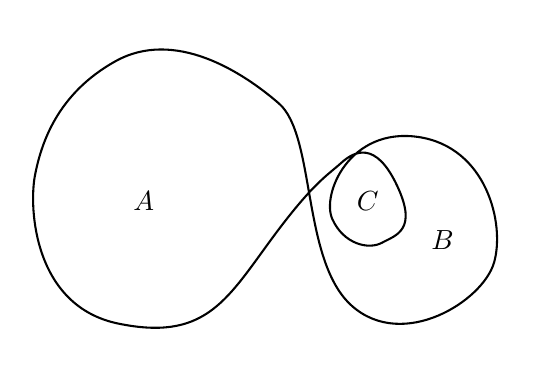
\begin{tikzpicture}[x=0.75pt,y=0.75pt,yscale=-1,xscale=1]
%uncomment if require: \path (0,162); %set diagram left start at 0, and has height of 162

%Shape: Polygon Curved [id:ds4706242055483567] 
\draw   (397.45,57.78) .. controls (364.48,52.98) and (350.69,85.35) .. (356.09,97.34) .. controls (361.48,109.33) and (373.47,112.33) .. (380.06,108.73) .. controls (386.66,105.13) and (397.45,102.74) .. (387.26,81.16) .. controls (377.07,59.58) and (366.88,64.37) .. (360.28,70.37) .. controls (353.69,76.36) and (346.49,79.96) .. (325.51,108.73) .. controls (304.53,137.5) and (293.74,156.09) .. (252.98,147.7) .. controls (212.22,139.3) and (209.82,91.95) .. (212.82,76.36) .. controls (215.82,60.78) and (223.61,36.8) .. (251.78,21.21) .. controls (279.96,5.63) and (312.33,26.01) .. (330.31,41.59) .. controls (348.29,57.18) and (341.1,117.72) .. (365.68,139.3) .. controls (390.25,160.88) and (428.62,136.91) .. (434.01,118.32) .. controls (439.41,99.74) and (430.42,62.57) .. (397.45,57.78) -- cycle ;

% Text Node
\draw (258.76,82.4) node [anchor=north west][inner sep=0.75pt]    {$A$};
% Text Node
\draw (402.33,101.24) node [anchor=north west][inner sep=0.75pt]    {$B$};
% Text Node
\draw (366.46,82.66) node [anchor=north west][inner sep=0.75pt]    {$C$};


\end{tikzpicture}

    \end{center}
    \end{vd}
    \begin{loigiai}
    Không mất tính tổng quát, giả sử rằng trong vòng $A$ thì dòng điện có chiều ngược chiều kim đồng hồ và từ thông qua $A$ dương. Dòng điện trong vòng dây bao quanh $C$ sẽ có chiều thuận chiều kim đồng hồ. Tương tự với dòng điện bao quanh $B$, lưu ý rằng diện tích vòng này là $B+C$. Từ thông qua các vòng này sẽ có giá trị âm. Từ thông qua cả vòng sẽ tỉ lệ với
    $$\phi \sim A-B-2C.$$
    Độ lớn suất điện động trong vòng dây sẽ là
    $$\varepsilon=\dfrac{-\dd B}{\dd t}(A-B-2C)=1.9\dv{V}.$$
    \end{loigiai}
    
    
    \begin{vd}[Chuyến phiêu lưu trên hòn đảo từ tính]
    Bên trong một hòn đảo hình elipse có bán trục nhỏ là $a=100\dv{m}$ và bán trục lớn $b=200\dv{m}$ có một vùng từ trường. Một chiếc xe ô tô có điện tích $Q=1.5\dv{C}$ chuyển động trên chu vi của hòn đảo với vận tốc có độ lớn không đổi $v=5\dv{m/s}$. Khối lượng của ô tô là $m=2000\dv{kg}$. Kích thước ô tô coi là rất bé so với kích thước hòn đảo. Bỏ qua từ trường gây ra bởi chiếc xe ô tô khi nó chuyển động và coi rằng ma sát đủ lớn để chiếc xe tiếp tục chuyển động trên quỹ đạo hình elipse.\\
    Chọn hệ tọa độ sao cho tâm hình học của hòn đảo nằm trên điểm có tọa đô $(0,0)$ và bán trục lớn và bán trục nhỏ của hòn đảo lần lượt nằm trên trục $Ox$ và trục $Oy$.\\
    Trên hòn đảo này, độ lớn cảm ứng từ trên hòn đảo phụ thuộc vào tọa độ $x$ và $y$ theo biểu thức $\ot{B}(x,y)=k_be^{c_bxy}\ot{k}$, với $\ot{k}$ là vector đơn vị theo trục $Oz$ có phương vuông góc với mặt phẳng và có hướng từ dưới lên trên. Các hằng số $c_b=10^{-4}\dv{m^{-2}}$ và $k_b=2.1\dv{\mu T}$.
    \begin{enumerate}[1)]
        \setlength\itemsep{0pt}
        \item Tại vị trí nào thì lực từ tác dụng lên chiếc xe ô tô là cực đại?
        \item Tại điểm có từ trường cực đại trên đường đi, tổng hợp lực tác dụng lên chiếc xe có giá trị là bao nhiêu?
    \end{enumerate}
    \end{vd}
    \begin{loigiai}
    Phương trình của đường elipse
    \[ \dfrac{x^2}{b^2}+\dfrac{y^2}{a^2}=1. \tag{1} \label{c91}\]
    \begin{enumerate}[1)]
        \setlength{\itemsep}{0pt}
        \item Vi phân hai vế của phương trình (\ref{c91}), ta được
        \[\begin{aligned}
                 &\dfrac{x\dd x}{b^2}+\dfrac{y\dd y}{a^2}=0\\
                 \Leftrightarrow  \ &\dd y=-\dfrac{a^2x}{b^2y}\dd x.
                \end{aligned}\tag{2} \label{c92}\]
        Ta có  
        \[\begin{aligned}
             B&=k_be^{c_bxy}\\
             \Leftrightarrow\  \dd B&=k_bc_bxe^{c_bxy}\dd y+k_bc_bye^{c_bxy}\dd x.
            \end{aligned}\tag{3} \label{c93} \]
        
        Kết hợp (\ref{c92}) và (\ref{c93}) ta được
        $$\dd B=k_bc_bxe^{c_bxy}\tron{-\dfrac{a^2x}{b^2y}\dd x}+k_bc_bye^{c_bxy}\dd x.$$
        Lực từ tác dụng lên xe 
        $F=Bvq$.\\
        Để lực từ đạt cực đại thì cảm ứng từ phải cực đại. Mà khi cảm ứng từ cực đại thì 
        \[\begin{aligned}
             \dd B=0\Leftrightarrow&\dfrac{a^2x^2}{b^2y}=y\\
             \Leftrightarrow& \dfrac{x^2}{b^2}=\dfrac{y^2}{b^2}. 
            \end{aligned}\tag{4}\label{c94}\]
        Từ (\ref{c91}) và (\ref{c94}) ta có
        \[\heva{{x^2} &= \frac{{{b^2}}}{2}\\  {y^2} &= \frac{{{a^2}}}{2} }\]
        Vậy các vị trí có lực từ cực đại là $A(141.4,70.7)$ và $B(-141.4,-70.7)$ với đơn vị là $\mathrm{m}$, đến trục $Ox$ là $70.7\dv{m}$.
        \item Phương trình quỹ đạo với những điểm có $x>0$, $y>0$
        $$y=\sqrt{1-\dfrac{a^2x^2}{b^2}}.$$
        \begin{center}
            
        {
\tikzset{every picture/.style={line width=0.75pt}} %set default line width to 0.75pt        

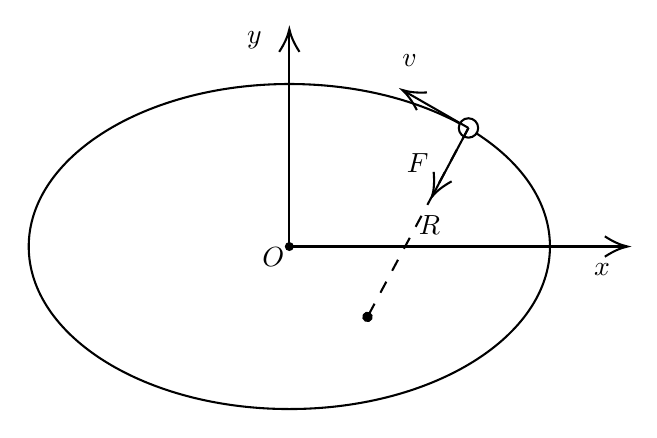
\begin{tikzpicture}[x=0.75pt,y=0.75pt,yscale=-1,xscale=1]
%uncomment if require: \path (0,231); %set diagram left start at 0, and has height of 231

%Straight Lines [id:da4337676199970719] 
\draw    (335.06,131.71) -- (335.06,29) ;
\draw [shift={(335.06,27)}, rotate = 450] [color={rgb, 255:red, 0; green, 0; blue, 0 }  ][line width=0.75]    (10.93,-4.9) .. controls (6.95,-2.3) and (3.31,-0.67) .. (0,0) .. controls (3.31,0.67) and (6.95,2.3) .. (10.93,4.9)   ;
%Straight Lines [id:da6548937942868309] 
\draw    (335.06,131.71) -- (496,131.71) ;
\draw [shift={(498,131.71)}, rotate = 180] [color={rgb, 255:red, 0; green, 0; blue, 0 }  ][line width=0.75]    (10.93,-4.9) .. controls (6.95,-2.3) and (3.31,-0.67) .. (0,0) .. controls (3.31,0.67) and (6.95,2.3) .. (10.93,4.9)   ;
%Shape: Arc [id:dp5326129500559582] 
\draw  [draw opacity=0] (335.12,53.41) .. controls (404.44,53.43) and (460.62,88.48) .. (460.62,131.71) .. controls (460.62,174.95) and (404.41,210.01) .. (335.06,210.01) .. controls (265.71,210.01) and (209.49,174.95) .. (209.49,131.71) .. controls (209.49,88.53) and (265.54,53.51) .. (334.76,53.41) -- (335.06,131.71) -- cycle ; \draw   (335.12,53.41) .. controls (404.44,53.43) and (460.62,88.48) .. (460.62,131.71) .. controls (460.62,174.95) and (404.41,210.01) .. (335.06,210.01) .. controls (265.71,210.01) and (209.49,174.95) .. (209.49,131.71) .. controls (209.49,88.53) and (265.54,53.51) .. (334.76,53.41) ;
%Shape: Ellipse [id:dp9199005088317054] 
\draw  [fill={rgb, 255:red, 0; green, 0; blue, 0 }  ,fill opacity=1 ] (333.42,131.71) .. controls (333.42,130.81) and (334.15,130.07) .. (335.06,130.07) .. controls (335.96,130.07) and (336.69,130.81) .. (336.69,131.71) .. controls (336.69,132.61) and (335.96,133.35) .. (335.06,133.35) .. controls (334.15,133.35) and (333.42,132.61) .. (333.42,131.71) -- cycle ;
%Shape: Ellipse [id:dp7599586645120926] 
\draw  [fill={rgb, 255:red, 255; green, 255; blue, 255 }  ,fill opacity=1 ] (416.69,74.59) .. controls (416.69,72.01) and (418.78,69.91) .. (421.36,69.91) .. controls (423.94,69.91) and (426.04,72.01) .. (426.04,74.59) .. controls (426.04,77.17) and (423.94,79.26) .. (421.36,79.26) .. controls (418.78,79.26) and (416.69,77.17) .. (416.69,74.59) -- cycle ;
%Straight Lines [id:da8609973334325589] 
\draw    (421.36,74.59) -- (391.19,57.28) ;
\draw [shift={(389.45,56.28)}, rotate = 389.84000000000003] [color={rgb, 255:red, 0; green, 0; blue, 0 }  ][line width=0.75]    (10.93,-4.9) .. controls (6.95,-2.3) and (3.31,-0.67) .. (0,0) .. controls (3.31,0.67) and (6.95,2.3) .. (10.93,4.9)   ;
%Straight Lines [id:da5341232523109551] 
\draw    (421.36,74.59) -- (404.72,105.9) ;
\draw [shift={(403.79,107.67)}, rotate = 297.98] [color={rgb, 255:red, 0; green, 0; blue, 0 }  ][line width=0.75]    (10.93,-4.9) .. controls (6.95,-2.3) and (3.31,-0.67) .. (0,0) .. controls (3.31,0.67) and (6.95,2.3) .. (10.93,4.9)   ;
%Straight Lines [id:da8503113451737665] 
\draw  [dash pattern={on 4.5pt off 4.5pt}]  (421.36,74.59) -- (372.71,165.62) ;
\draw [shift={(372.71,165.62)}, rotate = 118.12] [color={rgb, 255:red, 0; green, 0; blue, 0 }  ][fill={rgb, 255:red, 0; green, 0; blue, 0 }  ][line width=0.75]      (0, 0) circle [x radius= 2.01, y radius= 2.01]   ;

% Text Node
\draw (480.4,138.54) node [anchor=north west][inner sep=0.75pt]    {$x$};
% Text Node
\draw (313.27,26.77) node [anchor=north west][inner sep=0.75pt]    {$y$};
% Text Node
\draw (395.94,115.43) node [anchor=north west][inner sep=0.75pt]    {$R$};
% Text Node
\draw (388.04,37.58) node [anchor=north west][inner sep=0.75pt]    {$\ot{v}$};
% Text Node
\draw (320.61,130.96) node [anchor=north west][inner sep=0.75pt]    {$O$};
% Text Node
\draw (390.14,85.55) node [anchor=north west][inner sep=0.75pt]    {$\ot{F}$};
\end{tikzpicture}
}\end{center}
Bán kính chính khúc của một đường cong tại một điểm được tính theo biểu thức
        $$R=\dfrac{\tron{1+\tron{y'(x)}^2}^{\frac{3}{2}}}{\left|y''(x)\right|}.$$
 Ta có
        $$y'(x)=\dfrac{-\dfrac{a^2}{b^2}x}{\sqrt{1-\dfrac{a^2x^2}{b^2}}},$$
        $$y''(x)=\dfrac{-\dfrac{a^2}{b^2}}{\tron{1-\dfrac{a^2x^2}{b^2}}^{\frac{3}{2}}}.$$
        Tại điểm có lực từ cực đại
        $$R=\dfrac{\tron{a^2+b^2}^{\frac{3}{2}}}{2\sqrt{2}ab}=197.6\dv{m}.$$
        Tổng hợp lực tác dụng lên xe lúc đó
        $$F=m\frac{v^2}{R}=252.98\dv{N}.$$
    \end{enumerate}
    \end{loigiai}
    
    
    
\begin{vd}[Cải tiến cyclotron]
Cyclotron là máy gia tốc hạt tích điện có cấu tạo gồm hai hộp rỗng có dạng trụ nửa hình tròn gọi là các $D$, đặt cách nhau một khoảng rất nhỏ (khe). Máy được đặt trong một buồng đã hút hết không khí. Các $D$ được nối với nguồn điện có điện áp $u$ biên độ không đổi nhưng dấu thay đổi một cách tuần hoàn theo thời gian với tần số $f_0$. Một nam châm điện mạnh tạo ra một từ trường đều có vector cảm ứng từ $\ot{B}$ vuông góc với mặt các $D$.
Một hạt prôtôn có khối lượng nghỉ $m_0$, mang điện tích $e$ phát ra giữa hai thành khe, được gia tốc bởi máy cyclotron đến va đập vào bia như trên Hình vẽ.
\begin{center}
    

\tikzset{every picture/.style={line width=0.75pt}} %set default line width to 0.75pt        

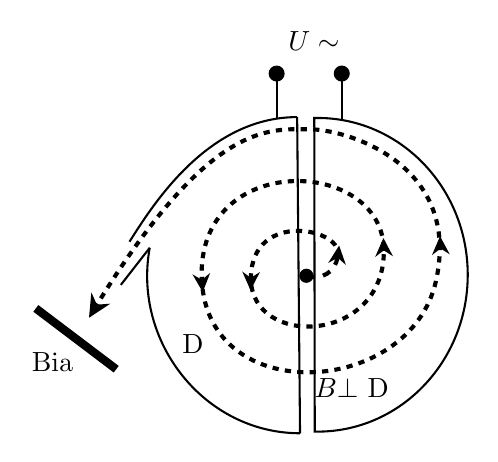
\begin{tikzpicture}[x=0.75pt,y=0.75pt,yscale=-1,xscale=1]
%uncomment if require: \path (0,300); %set diagram left start at 0, and has height of 300

%Curve Lines [id:da26455155450800905] 
\draw [line width=1.5]  [dash pattern={on 2.25pt off 2.25pt on 2.25pt off 2.25pt}]  (194.96,176.44) .. controls (250.39,85.57) and (279.06,89.84) .. (298.26,89.84) .. controls (317.76,89.84) and (372.08,107.42) .. (359.54,163.08) .. controls (347.01,218.74) and (249.51,224.6) .. (246.73,162.2) .. controls (243.94,99.8) and (334.47,103.02) .. (334.47,148.43) .. controls (334.47,193.84) and (270.24,195.21) .. (270.41,161.61) .. controls (270.57,128.01) and (316.32,137.78) .. (312.19,151.36) ;
\draw [shift={(192.41,180.65)}, rotate = 300.95] [fill={rgb, 255:red, 0; green, 0; blue, 0 }  ][line width=0.08]  [draw opacity=0] (11.07,-5.32) -- (0,0) -- (11.07,5.32) -- (7.35,0) -- cycle    ;
%Curve Lines [id:da3459025829014306] 
\draw [line width=1.5]  [dash pattern={on 3pt off 3pt on 3pt off 3pt}]  (312.19,151.36) .. controls (311.2,158.42) and (304.37,162.91) .. (297.15,160.44) ;
%Curve Lines [id:da9378209016899643] 
\draw [line width=0.75]    (294.08,236.31) .. controls (248.12,236.31) and (213.3,192.37) .. (221.66,146.96) ;
%Curve Lines [id:da46444033016051556] 
\draw [line width=0.75]    (211.91,144.03) .. controls (223.05,126.46) and (249.51,83.98) .. (292.69,83.98) ;
%Shape: Chord [id:dp4961973400604831] 
\draw   (300.94,84.41) .. controls (301.79,84.39) and (302.64,84.39) .. (303.5,84.4) .. controls (343.42,84.94) and (375.38,119.21) .. (374.87,160.94) .. controls (374.36,202.67) and (341.58,236.05) .. (301.65,235.51) .. controls (301.49,235.51) and (301.33,235.51) .. (301.17,235.5) -- cycle ;
%Straight Lines [id:da7151984865567858] 
\draw    (312.19,152.26) -- (312.57,148.84) ;
\draw [shift={(312.91,145.86)}, rotate = 456.41] [fill={rgb, 255:red, 0; green, 0; blue, 0 }  ][line width=0.08]  [draw opacity=0] (8.93,-4.29) -- (0,0) -- (8.93,4.29) -- (5.93,0) -- cycle    ;
%Straight Lines [id:da606634178835421] 
\draw    (270.41,161.61) -- (270.33,164.4) ;
\draw [shift={(270.24,167.4)}, rotate = 271.61] [fill={rgb, 255:red, 0; green, 0; blue, 0 }  ][line width=0.08]  [draw opacity=0] (8.93,-4.29) -- (0,0) -- (8.93,4.29) -- (5.93,0) -- cycle    ;
%Straight Lines [id:da13344562726382336] 
\draw    (246.73,162.2) -- (246.97,165.3) ;
\draw [shift={(247.21,168.29)}, rotate = 265.53] [fill={rgb, 255:red, 0; green, 0; blue, 0 }  ][line width=0.08]  [draw opacity=0] (8.93,-4.29) -- (0,0) -- (8.93,4.29) -- (5.93,0) -- cycle    ;
%Straight Lines [id:da7136597707124828] 
\draw    (334.47,148.43) -- (334.35,145.27) ;
\draw [shift={(334.24,142.27)}, rotate = 447.82] [fill={rgb, 255:red, 0; green, 0; blue, 0 }  ][line width=0.08]  [draw opacity=0] (8.93,-4.29) -- (0,0) -- (8.93,4.29) -- (5.93,0) -- cycle    ;
%Straight Lines [id:da6420109499040905] 
\draw    (361.79,146.96) -- (361.68,144.37) ;
\draw [shift={(361.54,141.37)}, rotate = 447.49] [fill={rgb, 255:red, 0; green, 0; blue, 0 }  ][line width=0.08]  [draw opacity=0] (8.93,-4.29) -- (0,0) -- (8.93,4.29) -- (5.93,0) -- cycle    ;
%Straight Lines [id:da6558307060262243] 
\draw    (221.66,146.96) -- (207.73,164.83) ;
%Straight Lines [id:da6529278329546151] 
\draw [line width=3]    (166.8,176.16) -- (205.52,205.45) ;
%Straight Lines [id:da808799244375606] 
\draw    (292.69,83.98) -- (294.08,236.31) ;
%Straight Lines [id:da3295166773899647] 
\draw    (282.81,63) -- (282.81,85) ;
\draw [shift={(282.81,63)}, rotate = 90] [color={rgb, 255:red, 0; green, 0; blue, 0 }  ][fill={rgb, 255:red, 0; green, 0; blue, 0 }  ][line width=0.75]      (0, 0) circle [x radius= 3.35, y radius= 3.35]   ;
%Straight Lines [id:da3895719018418451] 
\draw    (314.18,63) -- (314.18,85) ;
\draw [shift={(314.18,63)}, rotate = 90] [color={rgb, 255:red, 0; green, 0; blue, 0 }  ][fill={rgb, 255:red, 0; green, 0; blue, 0 }  ][line width=0.75]      (0, 0) circle [x radius= 3.35, y radius= 3.35]   ;
%Shape: Circle [id:dp06101742037391533] 
\draw  [fill={rgb, 255:red, 0; green, 0; blue, 0 }  ,fill opacity=1 ] (294.25,160.44) .. controls (294.25,158.84) and (295.55,157.54) .. (297.15,157.54) .. controls (298.75,157.54) and (300.05,158.84) .. (300.05,160.44) .. controls (300.05,162.04) and (298.75,163.34) .. (297.15,163.34) .. controls (295.55,163.34) and (294.25,162.04) .. (294.25,160.44) -- cycle ;


% Text Node
\draw (163.36,196) node [anchor=north west][inner sep=0.75pt]   [align=left] {Bia};
% Text Node
\draw (286.92,41.4) node [anchor=north west][inner sep=0.75pt]    {$U\sim $};
% Text Node
\draw (235.85,187.4) node [anchor=north west][inner sep=0.75pt]    {D};
% Text Node
\draw (299.57,208.4) node [anchor=north west][inner sep=0.75pt]    {$\ot{B} \bot$ D};


\end{tikzpicture}
\end{center}
\begin{enumerate}[1)]
    \item Khi hạt có tốc độ nhỏ, để đảm bảo sự đồng bộ (hạt luôn được điện trường tăng tốc khi đi qua khe) thì cảm ứng từ trong các D cần có trị số $B_0$ là bao nhiêu?     
    \item Khi hạt có tốc độ lớn mà tần số dòng xoay chiều và cảm ứng từ $B$ không đổi thì xuất hiện sự không đồng bộ cản trở sự tăng năng lượng của hạt. Để thực hiện sự đồng bộ, có thể có hai cách sau:
    \begin{enumerate}[a)]
        \item Thay đổi tần số $f$ của điện áp $u$, giữ nguyên biên độ điện áp và cảm ứng từ $B = B_0$. Chọn $t = 0$ là thời điểm hạt chuyển động với tần số $f_1$. Tìm quy luật thay đổi của $f$ theo thời gian $t$ để đảm bảo sự đồng bộ và sau mỗi vòng chuyển động năng lượng của hạt tăng thêm một lượng không đổi là $\Delta E$.       
        \item Thay đổi cảm ứng từ để tần số chuyển động của hạt luôn là $f_0$ không đổi. Hãy:
        \begin{itemize}
            \item Tìm quy luật thay đổi cảm ứng từ $B$ theo động năng $W$ của hạt.
            \item Tìm quy luật thay đổi bán kính quỹ đạo của hạt theo cảm ứng từ $B$.
        \end{itemize}
    \end{enumerate}
\end{enumerate}
\end{vd}

\begin{loigiai}
    \begin{enumerate}[1)]
        \item Với v nhỏ, tần số dòng xoay chiều bằng tần số quay của hạt trong từ trường: 
        \[e{{\omega }_{0}}R{{B}_{0}}={{m}_{0}}{{\omega }_{0}}^{2}R,\] suy ra \[{{\omega }_{0}}=\dfrac{e{{B}_{0}}}{{{m}_{0}}}=2\pi {{f}_{0}}.\] Tần số \[{{f}_{0}}=\dfrac{{{\omega }_{0}}}{2\pi }=\dfrac{e{{B}_{0}}}{2\pi {{m}_{0}}}, \tag{1} \label{tr.tst.4.1}\] 
        \[{{B}_{0}}=\dfrac{2\pi {{m}_{0}}{{f}_{0}}}{e}.\]
        \item \begin{enumerate}[a)]
            \item Với $v$ lớn, khối lượng hạt thay đổi theo vận tốc $m=\gamma {{m}_{0}}$, với $\gamma =\dfrac{1}{\sqrt{1-\dfrac{{{v}^{2}}}{{{c}^{2}}}}}.$
            \\Thay vào (\ref{tr.tst.4.1}) $f=\dfrac{{{f}_{0}}}{\gamma }$, ta có động năng 
            \[W={{m}_{0}}{{c}^{2}}(\gamma -1)={{m}_{0}}{{c}^{2}}\left( \dfrac{{{f}_{0}}}{f}-1 \right), \tag{2} \label{tr.tst.4.2}\] 
            suy ra \[\dfrac{W}{{{m}_{0}}{{c}^{2}}}=\dfrac{{{f}_{0}}}{f}-1.\] 
            Đạo hàm hai vế theo thời gian t: \[\dfrac{\dd W}{{\dd t}}=-{{m}_{0}}{{c}^{2}}\dfrac{{{f}_{0}}}{{{f}^{2}}}\dfrac{{\dd f}}{{\dd t}}=\Delta Ef.\] (trong 1s hạt quay được $f$ vòng,  sau mỗi vòng năng lượng tăng một lượng $\Delta E$). 
            \[-\dfrac{\dd f}{{{{f}}^{{3}}}}=\dfrac{\Delta {E}}{{{f}_{0}}{{m}_{0}}{{c}^{2}}}dt.\] Tích phân từ $0\to t$ ta có \[\dfrac{1}{2{{f}^{2}}}-\dfrac{1}{2f_{1}^{2}}=\dfrac{\Delta {E}.t}{{{f}_{0}}{{m}_{0}}{{c}^{2}}}.\]
            Biến đổi: \[f=\dfrac{{{f}_{1}}}{\sqrt{1+\dfrac{2f_{1}^{2}\Delta E\cdot t}{{{f}_{0}}{{m}_{0}}{{c}^{2}}}}}=\dfrac{{{f}_{1}}}{\sqrt{1+\dfrac{4\pi f_{1}^{2}\Delta E\cdot t}{e{{B}_{0}}{{c}^{2}}}}}.\]
            \item Viết lại (\ref{tr.tst.4.1}) \[f=\dfrac{eB}{2\pi \gamma {{m}_{0}}}={{f}_{0}}=\dfrac{e{{B}_{0}}}{2\pi {{m}_{0}}}\Rightarrow B=\gamma {{B}_{0}}. \tag{3} \label{tr.tst.4.3}\]
            Kết hợp với (\ref{tr.tst.4.2}) ta có: 
            \[B={{B}_{0}}\left( 1+\dfrac{W}{{{m}_{0}}{{c}^{2}}} \right).\]
            Bán kính quỹ đạo: \[r=\dfrac{mv}{eB}=\dfrac{\gamma {{m}_{0}}v}{\gamma e{{B}_{0}}}=\dfrac{{{m}_{0}}}{e{{B}_{0}}}\cdot v, \tag{4} \label{tr.tst.4.4} \]
            Từ (\ref{tr.tst.4.3}): \[{{\left( \dfrac{B}{{{B}_{0}}} \right)}^{2}}={{\gamma }^{2}}=\dfrac{1}{1-\dfrac{{{v}^{2}}}{{{c}^{2}}}}\Rightarrow \dfrac{{{v}^{2}}}{{{c}^{2}}}=1-{{\left( \dfrac{{{B}_{0}}}{B} \right)}^{2}}.\]
            Thay v và thế (\ref{tr.tst.4.1}) vào (\ref{tr.tst.4.4}) ta được  \[r=\dfrac{c}{2\pi {{f}_{0}}}\sqrt{1-{{\left( \dfrac{{{B}_{0}}}{B} \right)}^{2}}}=\dfrac{c}{2\pi {{f}_{0}}}\sqrt{1-{{\left( \dfrac{2\pi {{m}_{0}}{{f}_{0}}}{eB} \right)}^{2}}}.\]

        \end{enumerate}

    \end{enumerate}
\end{loigiai}


\begin{vd}[Dây hình gì?]
    Xét một vòng dây dẫn biến dạng tự do có vỏ bọc cách điện dài $2l$, có hai đầu được cố định vào trần nhà. Một vật nặng khối lượng $m$ được đặt cố định vào giữa dây (khối lượng của dây không đáng kể). Ngoài ra có một từ trường ngang cảm ứng $B$; gia tốc rơi tự do là $g$. Một dòng điện $I$ đang dẫn qua dây dẫn. Bỏ qua trường do dây dẫn gây ra.
    \begin{center}
        \tikzset{every picture/.style={line width=0.75pt}} %set default line width to 0.75pt        
        \begin{tikzpicture}[x=0.75pt,y=0.75pt,yscale=-1,xscale=1]
        \draw [line width=0.75]    (236,201) .. controls (252,172) and (242.4,225) .. (242.4,225) ;
        \draw  [fill={rgb, 255:red, 0; green, 0; blue, 0 }  ,fill opacity=1 ] (231.9,207) -- (256.9,207) -- (256.9,227) -- (231.9,227) -- cycle ;
        \draw    (197.58,67.31) -- (291,67.31) ;
        \draw  [draw opacity=0][fill={rgb, 255:red, 155; green, 155; blue, 155 }  ,fill opacity=0.6 ] (197.58,52) -- (291,52) -- (291,67.31) -- (197.58,67.31) -- cycle ;
        \draw [color={rgb, 255:red, 74; green, 144; blue, 226 }  ,draw opacity=1 ][line width=1.5]    (242.29,67.31) .. controls (226,241.2) and (262,239.2) .. (246.29,67.31) ;
        \draw    (231,128) -- (231,157) ;
        \draw [shift={(231,160)}, rotate = 270] [fill={rgb, 255:red, 0; green, 0; blue, 0 }  ][line width=0.08]  [draw opacity=0] (10.72,-5.15) -- (0,0) -- (10.72,5.15) -- (7.12,0) -- cycle    ;
        \draw    (258,123) -- (258,95.4) ;
        \draw [shift={(258,92.4)}, rotate = 450] [fill={rgb, 255:red, 0; green, 0; blue, 0 }  ][line width=0.08]  [draw opacity=0] (10.72,-5.15) -- (0,0) -- (10.72,5.15) -- (7.12,0) -- cycle    ;
        \draw   (272.5,143) .. controls (272.5,136.65) and (277.65,131.5) .. (284,131.5) .. controls (290.35,131.5) and (295.5,136.65) .. (295.5,143) .. controls (295.5,149.35) and (290.35,154.5) .. (284,154.5) .. controls (277.65,154.5) and (272.5,149.35) .. (272.5,143) -- cycle ;
        \draw  [fill={rgb, 255:red, 0; green, 0; blue, 0 }  ,fill opacity=1 ] (280.75,143) .. controls (280.75,141.21) and (282.21,139.75) .. (284,139.75) .. controls (285.79,139.75) and (287.25,141.21) .. (287.25,143) .. controls (287.25,144.79) and (285.79,146.25) .. (284,146.25) .. controls (282.21,146.25) and (280.75,144.79) .. (280.75,143) -- cycle ;
        % Text Node
        \draw (237,212.4) node [anchor=north west][inner sep=0.75pt]  [color={rgb, 255:red, 255; green, 255; blue, 255 }  ,opacity=1 ]  {$m$};
        % Text Node
        \draw (218,134.4) node [anchor=north west][inner sep=0.75pt]    {$I$};
        % Text Node
        \draw (262,105.4) node [anchor=north west][inner sep=0.75pt]    {$I$};
        % Text Node
        \draw (286,157.9) node [anchor=north west][inner sep=0.75pt]    {$\ot{B}$};
        \end{tikzpicture}
    \end{center}
    \begin{enumerate}[1)]
        \item Vẽ phác họa hình dạng của dây.
        \item Tìm độ cao tối đa mà vật nặng có thể đạt được (có thể tăng dòng điện).
        \item Viết phương trình xác định độ biến thiên chiều cao $\Delta h$.
        \item Cường độ dòng điện cần đạt giá trị $I_0$ bằng bao nhiêu để vật dịch chuyển $\Delta h_0= l\left(1-\dfrac{3}{\pi}\right)$?
    \end{enumerate}
\end{vd}
\begin{loigiai}
    \begin{enumerate}[1)]
        \item Lực Ampe kéo dây sang một bên để dây có dạng cong. Vì lực Ampe có phương vuông góc với dây nên lực căng không đổi dọc theo dây dẫn. 
        \\Gọi lực căng là $T$ và bán kính cong của dây tại một điểm xác định là $R$. 
        \\Ta xét một đoạn dây rất ngắn có chiều dài $a \ll R$. 
        \\Khi đó, $\alpha = \dfrac{a}{R} $. 
        \\Ta phân tích các lực cân bằng theo phương vuông góc với dây: Lực Ampe cân bằng với hợp lực của hai lực căng $T$ tác dụng lên hai đầu đoạn dây.
        \begin{center}
            \tikzset{every picture/.style={line width=0.75pt}} %set default line width to 0.75pt        
            \begin{tikzpicture}[x=0.75pt,y=0.75pt,yscale=-1,xscale=1]
            \draw  [draw opacity=0][line width=1.5]  (141.18,104.69) .. controls (162.32,117.21) and (176.49,140.25) .. (176.49,166.61) .. controls (176.49,192.58) and (162.72,215.35) .. (142.07,227.98) -- (104.59,166.61) -- cycle ; \draw  [color={rgb, 255:red, 74; green, 144; blue, 226 }  ,draw opacity=1 ][line width=1.5]  (141.18,104.69) .. controls (162.32,117.21) and (176.49,140.25) .. (176.49,166.61) .. controls (176.49,192.58) and (162.72,215.35) .. (142.07,227.98) ;
            \draw [line width=1.5]    (131.03,230.34) .. controls (149.52,196.82) and (138.43,258.08) .. (138.43,258.08) ;
            \draw  [draw opacity=0][line width=1.5]  (140.91,227.98) .. controls (119.77,215.46) and (105.6,192.42) .. (105.6,166.07) .. controls (105.6,140.09) and (119.37,117.33) .. (140.02,104.69) -- (177.5,166.07) -- cycle ; \draw  [color={rgb, 255:red, 74; green, 144; blue, 226 }  ,draw opacity=1 ][line width=1.5]  (140.91,227.98) .. controls (119.77,215.46) and (105.6,192.42) .. (105.6,166.07) .. controls (105.6,140.09) and (119.37,117.33) .. (140.02,104.69) ;
            \draw    (87.77,104.69) -- (195.76,104.69) ;
            %Shape: Rectangle [id:dp6849127090568536] 
            \draw  [fill={rgb, 255:red, 0; green, 0; blue, 0 }  ,fill opacity=1 ] (126.35,247.18) -- (150.5,247.18) -- (150.5,268.98) -- (126.35,268.98) -- cycle ;
            %Shape: Rectangle [id:dp20544103277538373] 
            \draw  [draw opacity=0][fill={rgb, 255:red, 155; green, 155; blue, 155 }  ,fill opacity=0.6 ] (87.77,87) -- (195.76,87) -- (195.76,104.69) -- (87.77,104.69) -- cycle ;
            %Shape: Arc [id:dp8227182968337245] 
            \draw  [draw opacity=0][line width=3]  (383.59,159.68) .. controls (385.82,168.79) and (387,178.31) .. (387,188.1) .. controls (387,195.11) and (386.4,201.98) .. (385.23,208.66) -- (267.9,188.1) -- cycle ; \draw  [color={rgb, 255:red, 74; green, 144; blue, 226 }  ,draw opacity=1 ][line width=3]  (383.59,159.68) .. controls (385.82,168.79) and (387,178.31) .. (387,188.1) .. controls (387,195.11) and (386.4,201.98) .. (385.23,208.66) ;
            %Straight Lines [id:da7872101289914] 
            \draw    (386.62,184.27) -- (420,184.27) ;
            \draw [shift={(423,184.27)}, rotate = 180] [fill={rgb, 255:red, 0; green, 0; blue, 0 }  ][line width=0.08]  [draw opacity=0] (8.93,-4.29) -- (0,0) -- (8.93,4.29) -- (5.93,0) -- cycle    ;
            %Straight Lines [id:da21347274525961635] 
            \draw    (388.53,184.27) -- (373.75,102.2) ;
            \draw [shift={(373.22,99.25)}, rotate = 439.79] [fill={rgb, 255:red, 0; green, 0; blue, 0 }  ][line width=0.08]  [draw opacity=0] (8.93,-4.29) -- (0,0) -- (8.93,4.29) -- (5.93,0) -- cycle    ;
            %Straight Lines [id:da2625800054969636] 
            \draw    (388.53,184.27) -- (377.47,260.96) ;
            \draw [shift={(377.04,263.93)}, rotate = 278.21] [fill={rgb, 255:red, 0; green, 0; blue, 0 }  ][line width=0.08]  [draw opacity=0] (8.93,-4.29) -- (0,0) -- (8.93,4.29) -- (5.93,0) -- cycle    ;
            %Straight Lines [id:da9313653241617372] 
            \draw    (388.53,184.27) -- (357.07,184.27) ;
            \draw [shift={(354.07,184.27)}, rotate = 360] [fill={rgb, 255:red, 0; green, 0; blue, 0 }  ][line width=0.08]  [draw opacity=0] (8.93,-4.29) -- (0,0) -- (8.93,4.29) -- (5.93,0) -- cycle    ;
            %Straight Lines [id:da31479179755094666] 
            \draw  [dash pattern={on 4.5pt off 4.5pt}]  (354.07,184.27) -- (373.22,99.25) ;
            %Straight Lines [id:da2096108846937219] 
            \draw  [dash pattern={on 4.5pt off 4.5pt}]  (377.04,263.93) -- (354.07,184.27) ;
            %Straight Lines [id:da59923207589652] 
            \draw  [dash pattern={on 0.84pt off 2.51pt}]  (267.9,188.1) -- (383.59,159.68) ;
            %Straight Lines [id:da8380472037322189] 
            \draw  [dash pattern={on 0.84pt off 2.51pt}]  (267.9,188.1) -- (385.23,208.66) ;
            %Shape: Arc [id:dp0317619181235802] 
            \draw  [draw opacity=0] (308.45,177.35) .. controls (310.03,180.37) and (310.93,183.64) .. (311.01,187.05) .. controls (311.08,189.93) and (310.57,192.72) .. (309.56,195.38) -- (267.9,188.1) -- cycle ; \draw   (308.45,177.35) .. controls (310.03,180.37) and (310.93,183.64) .. (311.01,187.05) .. controls (311.08,189.93) and (310.57,192.72) .. (309.56,195.38) ;
            %Straight Lines [id:da0809350954724033] 
            \draw    (172,162) -- (182,161.6) ;
            %Straight Lines [id:da09562099207543429] 
            \draw    (172,169.6) -- (182,169.6) ;
            %Straight Lines [id:da7045842076714772] 
            \draw    (192.8,165.8) -- (254.81,171.52) ;
            \draw [shift={(257.8,171.8)}, rotate = 185.27] [fill={rgb, 255:red, 0; green, 0; blue, 0 }  ][line width=0.08]  [draw opacity=0] (10.72,-5.15) -- (0,0) -- (10.72,5.15) -- (7.12,0) -- cycle    ;
            
            
            % Text Node
            \draw (314.4,176.48) node [anchor=north west][inner sep=0.75pt]    {$\alpha $};
            % Text Node
            \draw (385,128.4) node [anchor=north west][inner sep=0.75pt]    {$T$};
            % Text Node
            \draw (384.79,227.5) node [anchor=north west][inner sep=0.75pt]    {$T$};
            % Text Node
            \draw (396,184.4) node [anchor=north west][inner sep=0.75pt]    {$F_{A}$};
            % Text Node
            \draw (182,140.4) node [anchor=north west][inner sep=0.75pt]    {$a\ll l$};

            \end{tikzpicture}
        \end{center}
        Lực Ampe $F_A=IaB$ cân bằng với hợp lực căng  $T.\alpha=T\dfrac{a}{R}$.\\
        Vì vậy, $R=\dfrac{T}{IB}$, điều đó có nghĩa là $R$ là như nhau tại mọi điểm trên dây.
        \\ Vậy hai nửa dây sẽ có dạng cung tròn.
        \item Chiều cao tối đa vật đạt được khi hai đoạn tròn tạo thành một vòng tròn hoàn hảo.      
            \begin{center}
            \tikzset{every picture/.style={line width=0.75pt}} %set default line width to 0.75pt        
            \begin{tikzpicture}[x=0.75pt,y=0.75pt,yscale=-1,xscale=1]
            %uncomment if require: \path (0,300); %set diagram left start at 0, and has height of 300
            %Curve Lines [id:da9201622752984537] 
            \draw [line width=0.75]    (164,226) .. controls (180,197) and (170.4,250) .. (170.4,250) ;
            %Shape: Rectangle [id:dp8892251442654298] 
            \draw  [fill={rgb, 255:red, 0; green, 0; blue, 0 }  ,fill opacity=1 ] (159.9,232) -- (184.9,232) -- (184.9,252) -- (159.9,252) -- cycle ;
            
            %Straight Lines [id:da5663116008374898] 
            \draw    (121.58,83.31) -- (215,83.31) ;
            %Shape: Rectangle [id:dp3839281310668292] 
            \draw  [draw opacity=0][fill={rgb, 255:red, 155; green, 155; blue, 155 }  ,fill opacity=0.6 ] (121.58,68) -- (215,68) -- (215,83.31) -- (121.58,83.31) -- cycle ;
            %Curve Lines [id:da6443075343304285] 
            \draw [color={rgb, 255:red, 74; green, 144; blue, 226 }  ,draw opacity=1 ][line width=1.5]    (168.29,83.31) .. controls (164,266.2) and (179,262.2) .. (171.29,83.31) ;
            %Straight Lines [id:da1552793439917377] 
            \draw    (241.58,82.31) -- (335,82.31) ;
            %Shape: Rectangle [id:dp8529237826357821] 
            \draw  [draw opacity=0][fill={rgb, 255:red, 155; green, 155; blue, 155 }  ,fill opacity=0.6 ] (241.58,67) -- (335,67) -- (335,82.31) -- (241.58,82.31) -- cycle ;
            %Shape: Circle [id:dp8980566863976338] 
            \draw  [color={rgb, 255:red, 74; green, 144; blue, 226 }  ,draw opacity=1 ][line width=1.5]  (247.84,122.75) .. controls (247.84,100.42) and (265.95,82.31) .. (288.29,82.31) .. controls (310.63,82.31) and (328.74,100.42) .. (328.74,122.75) .. controls (328.74,145.09) and (310.63,163.2) .. (288.29,163.2) .. controls (265.95,163.2) and (247.84,145.09) .. (247.84,122.75) -- cycle ;
            %Curve Lines [id:da15102689800912072] 
            \draw [line width=0.75]    (282,170) .. controls (298,141) and (288.4,194) .. (288.4,194) ;
            %Shape: Rectangle [id:dp07205759967128311] 
            \draw  [fill={rgb, 255:red, 0; green, 0; blue, 0 }  ,fill opacity=1 ] (277.9,176) -- (302.9,176) -- (302.9,196) -- (277.9,196) -- cycle ;
            
            %Straight Lines [id:da6168278467988717] 
            \draw    (227.2,189) -- (227.2,243) ;
            \draw [shift={(227.2,246)}, rotate = 270] [fill={rgb, 255:red, 0; green, 0; blue, 0 }  ][line width=0.08]  [draw opacity=0] (10.72,-5.15) -- (0,0) -- (10.72,5.15) -- (7.12,0) -- cycle    ;
            \draw [shift={(227.2,186)}, rotate = 90] [fill={rgb, 255:red, 0; green, 0; blue, 0 }  ][line width=0.08]  [draw opacity=0] (10.72,-5.15) -- (0,0) -- (10.72,5.15) -- (7.12,0) -- cycle    ;
            %Straight Lines [id:da6510039046054072] 
            \draw    (288.29,125.75) -- (288.29,160.2) ;
            \draw [shift={(288.29,163.2)}, rotate = 270] [fill={rgb, 255:red, 0; green, 0; blue, 0 }  ][line width=0.08]  [draw opacity=0] (8.93,-4.29) -- (0,0) -- (8.93,4.29) -- (5.93,0) -- cycle    ;
            \draw [shift={(288.29,122.75)}, rotate = 90] [fill={rgb, 255:red, 0; green, 0; blue, 0 }  ][line width=0.08]  [draw opacity=0] (8.93,-4.29) -- (0,0) -- (8.93,4.29) -- (5.93,0) -- cycle    ;
            
            % Text Node
            \draw (165,231.4) node [anchor=north west][inner sep=0.75pt]  [color={rgb, 255:red, 255; green, 255; blue, 255 }  ,opacity=1 ]  {$m$};
            % Text Node
            \draw (152,147.4) node [anchor=north west][inner sep=0.75pt]    {$l$};
            % Text Node
            \draw (283,175.4) node [anchor=north west][inner sep=0.75pt]  [color={rgb, 255:red, 255; green, 255; blue, 255 }  ,opacity=1 ]  {$m$};
            % Text Node
            \draw (232.2,206.4) node [anchor=north west][inner sep=0.75pt]    {$\Delta h_{\max}$};
            % Text Node
            \draw (290.29,133.15) node [anchor=north west][inner sep=0.75pt]    {$l/\pi $};
            \end{tikzpicture}
        \end{center}
        Khi đó, vật đi lên một đoạn:
        \[\Delta h_{\max}=l\left(1-\dfrac{2}{\pi}\right)\]
        \item Nếu góc ở tâm của các đoạn tròn là $2\alpha$ thì tiếp tuyến của dây tại điểm treo vật tạo thành góc $\alpha$ với phương thẳng đứng. Vậy ta có phương trình cân bằng lực:
        \[mg=2T\cos\alpha.\]
        Mặt khác $R=\dfrac{l}{2\alpha}=\dfrac{T}{IB}$, ta có phương trình xác định góc $\alpha$:
        \[\alpha \dfrac{mg}{lIB}=\cos\alpha.\]
        Từ đó ta tìm được:
        \[\Delta h=l-2R\sin\alpha=l-\dfrac{2T}{lIB}\sin\alpha=l\left(1-\dfrac{\sin\alpha}{\alpha}\right).\]
        \item Từ kết quả ý trước, ta thấy $\Delta h=\Delta h_0=l\left(1-\dfrac{3}{\pi}\right)$
        thì 
        $$\dfrac{\sin\alpha}{\alpha}=\dfrac{\pi}{3}$$
        hay 
        $$\alpha=\dfrac{\pi}{6}.$$
        Khi đó 
        \[I=I_0=\dfrac{mg\alpha}{lB\cos\alpha}=\dfrac{mg\pi}{3\sqrt{3}lB}.\]
    \end{enumerate}
\end{loigiai} 

\begin{vd}[Tương tác nam châm]%Câu 5
Một nam châm $A$ rất ngắn với khối lượng $m$ được treo nằm ngang bởi một dây dài $l=1 \mathrm{m}$. Một nam châm $B$ khác cũng rất ngắn được dịch gần vào $A$ một cách chậm rãi sao cho trục của các nam châm luôn luôn nằm trên cùng đường thẳng nằm ngang. Khi khoảng cách giữa các nam châm là $d=4 \mathrm{cm}$, và nam châm A cách vị trí ban đầu một khoảng $s=1 \mathrm{cm}$, thì $A$ đột ngột dịch chuyển, tự gắn vào $B$.
\begin{center}
    

\tikzset{every picture/.style={line width=0.75pt}} %set default line width to 0.75pt        

\begin{tikzpicture}[x=0.75pt,y=0.75pt,yscale=-1,xscale=1]
%uncomment if require: \path (0,405); %set diagram left start at 0, and has height of 405

%Straight Lines [id:da7483648183576237] 
\draw    (181,19) -- (226,19) ;
%Straight Lines [id:da6768240988149081] 
\draw  [dash pattern={on 4.5pt off 4.5pt}]  (203.5,19) -- (203.5,322) ;
%Straight Lines [id:da30289391033730406] 
\draw    (203.5,19) -- (233,297) ;
%Shape: Rectangle [id:dp28470973440179037] 
\draw   (219.67,296) -- (233.17,296) -- (233.17,304) -- (219.67,304) -- cycle ;
%Shape: Rectangle [id:dp03262988764205854] 
\draw  [fill={rgb, 255:red, 0; green, 0; blue, 0 }  ,fill opacity=1 ] (233.17,296) -- (246.67,296) -- (246.67,304) -- (233.17,304) -- cycle ;

%Shape: Rectangle [id:dp6001524937136158] 
\draw   (282.67,295) -- (296.17,295) -- (296.17,303) -- (282.67,303) -- cycle ;
%Shape: Rectangle [id:dp8518561606495823] 
\draw  [fill={rgb, 255:red, 0; green, 0; blue, 0 }  ,fill opacity=1 ] (296.17,295) -- (309.67,295) -- (309.67,303) -- (296.17,303) -- cycle ;

%Straight Lines [id:da7419816758599442] 
\draw  [dash pattern={on 4.5pt off 4.5pt}]  (233.17,304) -- (233.17,323) ;
%Straight Lines [id:da6001151727751939] 
\draw  [dash pattern={on 4.5pt off 4.5pt}]  (296.17,303) -- (296.17,322) ;
%Straight Lines [id:da19540711893532214] 
\draw    (207,316) -- (229,316) ;
\draw [shift={(232,316)}, rotate = 180] [fill={rgb, 255:red, 0; green, 0; blue, 0 }  ][line width=0.08]  [draw opacity=0] (10.72,-5.15) -- (0,0) -- (10.72,5.15) -- (7.12,0) -- cycle    ;
\draw [shift={(204,316)}, rotate = 0] [fill={rgb, 255:red, 0; green, 0; blue, 0 }  ][line width=0.08]  [draw opacity=0] (10.72,-5.15) -- (0,0) -- (10.72,5.15) -- (7.12,0) -- cycle    ;
%Straight Lines [id:da5634621604200039] 
\draw    (235,316) -- (295,316) ;
\draw [shift={(298,316)}, rotate = 180] [fill={rgb, 255:red, 0; green, 0; blue, 0 }  ][line width=0.08]  [draw opacity=0] (10.72,-5.15) -- (0,0) -- (10.72,5.15) -- (7.12,0) -- cycle    ;
\draw [shift={(232,316)}, rotate = 0] [fill={rgb, 255:red, 0; green, 0; blue, 0 }  ][line width=0.08]  [draw opacity=0] (10.72,-5.15) -- (0,0) -- (10.72,5.15) -- (7.12,0) -- cycle    ;

% Text Node
\draw (212,320.4) node [anchor=north west][inner sep=0.75pt]    {$s$};
% Text Node
\draw (258,316.4) node [anchor=north west][inner sep=0.75pt]    {$d$};
% Text Node
\draw (237,274.4) node [anchor=north west][inner sep=0.75pt]    {$A$};
% Text Node
\draw (294,273.4) node [anchor=north west][inner sep=0.75pt]    {$B$};
% Text Node
\draw (225,154.4) node [anchor=north west][inner sep=0.75pt]    {$l$};


\end{tikzpicture}

\end{center}
\begin{enumerate}[1)]
    \item Lực tương tác giữa các nam châm phụ thuộc vào khoảng cách theo liên hệ $F_{nc}(x)=\pm\dfrac{K}{x^n}$, dấu cộng hay trừ phụ thuộc vào hướng của các nam châm so với nhau. Sử dụng các thông tin đã cho, tìm giá trị của $n$.
    \item Đặt nam châm $B$ vào trong một ống thủy tinh thẳng đứng, kín đầu dưới. Và nam châm $A$ được đặt ngay trên nó, ở bên trong ống sao cho hai nam châm đẩy nhau. Có thể nam châm $A$ có xu hướng đảo chiều lại, nhưng nó đã bị ràng buộc bởi ống nên trường hợp đó không xảy ra. Hãy tìm khoảng cách giữa các nam châm trong trạng thái cân bằng.
\end{enumerate}

\end{vd}
\begin{loigiai}
\begin{enumerate}[1)]
    \item Thành phần tổng hợp lực theo phương ngang (chiều dương theo hướng mà $x$ tăng, hay nói cách khác, hướng bên trái của hình vẽ trong đề bài) tác dụng lên nam châm $A$ là:
	 \[F(x)=-\dfrac{K}{x^n}+mg\dfrac{d+s-x}{l}, \tag{1} \]
với $d+s$ là khoảng cách từ nam châm $B$ tới vị trí không chịu tác động của nam châm $A$. Điều kiện cân bằng:
	\[ F\left(x=d\right)=0. \tag{2}\]
Cân bằng có bền hay không phụ thuộc vào tính chất của hàm $F(x)$ tại khoảng giá trị gần $x=d$. Hàm này có thể là hàm đơn điệu tăng hoặc giảm (Hình vẽ).

    

	
\begin{center}


\tikzset{every picture/.style={line width=0.75pt}} %set default line width to 0.75pt        

\begin{tikzpicture}[x=0.75pt,y=0.75pt,yscale=-1,xscale=1]
%uncomment if require: \path (0,429); %set diagram left start at 0, and has height of 429

%Straight Lines [id:da7602690314536287] 
\draw    (160,330) -- (387,330) ;
\draw [shift={(390,330)}, rotate = 180] [fill={rgb, 255:red, 0; green, 0; blue, 0 }  ][line width=0.08]  [draw opacity=0] (10.72,-5.15) -- (0,0) -- (10.72,5.15) -- (7.12,0) -- cycle    ;
%Straight Lines [id:da2500833984576549] 
\draw    (178,348) -- (178,179) ;
\draw [shift={(178,176)}, rotate = 450] [fill={rgb, 255:red, 0; green, 0; blue, 0 }  ][line width=0.08]  [draw opacity=0] (10.72,-5.15) -- (0,0) -- (10.72,5.15) -- (7.12,0) -- cycle    ;
%Curve Lines [id:da961445292848941] 
\draw    (233,274) .. controls (288,306) and (323,379) .. (317,378) ;
%Curve Lines [id:da4693557200247729] 
\draw    (249,377) .. controls (277,338) and (344,283) .. (367,284) ;
%Shape: Circle [id:dp8884936741023908] 
\draw  [fill={rgb, 255:red, 0; green, 0; blue, 0 }  ,fill opacity=1 ] (289,331) .. controls (289,329.34) and (290.34,328) .. (292,328) .. controls (293.66,328) and (295,329.34) .. (295,331) .. controls (295,332.66) and (293.66,334) .. (292,334) .. controls (290.34,334) and (289,332.66) .. (289,331) -- cycle ;

% Text Node
\draw (151,155.4) node [anchor=north west][inner sep=0.75pt]    {$F( x)$};
% Text Node
\draw (392,333.4) node [anchor=north west][inner sep=0.75pt]    {$x$};
% Text Node
\draw (348,262.4) node [anchor=north west][inner sep=0.75pt]    {$Unstable$};
% Text Node
\draw (217,254.4) node [anchor=north west][inner sep=0.75pt]    {$Stable$};


\end{tikzpicture}

\end{center}

Đối với cân bằng bền, đạo hàm của hàm lực phải âm. Còn với cân bằng không bền thì dương, và trong trường hợp cân bằng phiếm định là $0$, tức
	\[ F'\left(x=d\right)=0.	\tag{3}\]
Sử dụng biểu thức (1) của lực $F(x)$, điều kiện (3) có thể được viết dưới dạng:
	 \[\dfrac{nK}{d^{n+1}}-\dfrac{mg}{l}=0. \tag{4} \]
Trong khi điều kiện (2) thì có thể viết dưới dạng:
	 \[-\dfrac{K}{d^n}+\dfrac{mg}{l}s=0.	\]
Từ những phương trình trên, ta thu được:
	 \[n=\dfrac{d}{s}=4.\] và  \[K=mg{d^4}\dfrac{s}{l}. \tag{6}\]
	\item Trong ống thẳng đứng (Hình vẽ) lực đẩy tác dụng lên nam châm $A$ là: $$F_d(x)=\dfrac{K}{x^4}-mg.$$
\begin{center}
    

\tikzset{every picture/.style={line width=0.75pt}} %set default line width to 0.75pt        

\begin{tikzpicture}[x=0.75pt,y=0.75pt,yscale=-1,xscale=1]
%uncomment if require: \path (0,454); %set diagram left start at 0, and has height of 454

%Shape: Arc [id:dp49952120378007514] 
\draw  [draw opacity=0] (225.99,313.04) .. controls (226,313.19) and (226,313.35) .. (226,313.5) .. controls (226,324.27) and (216.37,333) .. (204.5,333) .. controls (192.63,333) and (183,324.27) .. (183,313.5) .. controls (183,313.35) and (183,313.19) .. (183.01,313.04) -- (204.5,313.5) -- cycle ; \draw   (225.99,313.04) .. controls (226,313.19) and (226,313.35) .. (226,313.5) .. controls (226,324.27) and (216.37,333) .. (204.5,333) .. controls (192.63,333) and (183,324.27) .. (183,313.5) .. controls (183,313.35) and (183,313.19) .. (183.01,313.04) ;
%Shape: Arc [id:dp11432984532966284] 
\draw  [draw opacity=0] (220.5,313.77) .. controls (220.35,321.93) and (213.24,328.5) .. (204.5,328.5) .. controls (195.75,328.5) and (188.65,321.92) .. (188.5,313.75) -- (204.5,313.5) -- cycle ; \draw   (220.5,313.77) .. controls (220.35,321.93) and (213.24,328.5) .. (204.5,328.5) .. controls (195.75,328.5) and (188.65,321.92) .. (188.5,313.75) ;
%Straight Lines [id:da29864369798265167] 
\draw    (188.5,139.5) -- (188.5,313.75) ;
%Straight Lines [id:da88747493933312] 
\draw    (220.5,139.77) -- (220.5,313.77) ;
%Straight Lines [id:da9397137932142579] 
\draw    (183.01,139) -- (183.01,313.04) ;
%Straight Lines [id:da46085076434842787] 
\draw    (225.99,139) -- (225.99,313.04) ;
%Shape: Rectangle [id:dp34187514257755547] 
\draw   (210.17,159.5) -- (210.17,175.92) -- (199,175.92) -- (199,159.5) -- cycle ;
%Shape: Rectangle [id:dp12055191944000243] 
\draw  [fill={rgb, 255:red, 0; green, 0; blue, 0 }  ,fill opacity=1 ] (210.17,175.92) -- (210.17,192.33) -- (199,192.33) -- (199,175.92) -- cycle ;

%Shape: Rectangle [id:dp1663810616516499] 
\draw   (199,322.5) -- (199,307.75) -- (209.83,307.75) -- (209.83,322.5) -- cycle ;
%Shape: Rectangle [id:dp007472288684529316] 
\draw  [fill={rgb, 255:red, 0; green, 0; blue, 0 }  ,fill opacity=1 ] (199,307.75) -- (199,293) -- (209.83,293) -- (209.83,307.75) -- cycle ;

%Straight Lines [id:da02169932115940343] 
\draw    (205,160.33) -- (205,110.33) ;
\draw [shift={(205,107.33)}, rotate = 450] [fill={rgb, 255:red, 0; green, 0; blue, 0 }  ][line width=0.08]  [draw opacity=0] (10.72,-5.15) -- (0,0) -- (10.72,5.15) -- (7.12,0) -- cycle    ;
%Straight Lines [id:da6684588777762237] 
\draw    (204.67,191) -- (204.67,234.67) ;
\draw [shift={(204.67,237.67)}, rotate = 270] [fill={rgb, 255:red, 0; green, 0; blue, 0 }  ][line width=0.08]  [draw opacity=0] (10.72,-5.15) -- (0,0) -- (10.72,5.15) -- (7.12,0) -- cycle    ;
%Straight Lines [id:da8074211952133599] 
\draw  [dash pattern={on 4.5pt off 4.5pt}]  (227,176) -- (253,176) ;
%Straight Lines [id:da7029621782700632] 
\draw  [dash pattern={on 4.5pt off 4.5pt}]  (227,308) -- (253,308) ;
%Straight Lines [id:da17037311528522747] 
\draw    (240,179) -- (240,305) ;
\draw [shift={(240,308)}, rotate = 270] [fill={rgb, 255:red, 0; green, 0; blue, 0 }  ][line width=0.08]  [draw opacity=0] (10.72,-5.15) -- (0,0) -- (10.72,5.15) -- (7.12,0) -- cycle    ;
\draw [shift={(240,176)}, rotate = 90] [fill={rgb, 255:red, 0; green, 0; blue, 0 }  ][line width=0.08]  [draw opacity=0] (10.72,-5.15) -- (0,0) -- (10.72,5.15) -- (7.12,0) -- cycle    ;

% Text Node
\draw (160,167.4) node [anchor=north west][inner sep=0.75pt]    {$A$};
% Text Node
\draw (156,215.4) node [anchor=north west][inner sep=0.75pt]    {$mg$};
% Text Node
\draw (212,82.4) node [anchor=north west][inner sep=0.75pt]    {$\dfrac{K}{h^{4}}$};
% Text Node
\draw (247,232.4) node [anchor=north west][inner sep=0.75pt]    {$h$};
% Text Node
\draw (164,300.4) node [anchor=north west][inner sep=0.75pt]    {$B$};


\end{tikzpicture}

\end{center}

Hệ sẽ đạt được điều kiện cân bằng lơ lửng khi các nam châm cách nhau một khoảng $h$, với
\[F_d\left(x=h\right)=0.\]
Sử dụng kết quả (6) cho ta:
\[h = {\left( {\dfrac{K}{{mg}}} \right)^{\frac{1}{4}}} = d{\left( {\dfrac{s}{l}} \right)^{\frac{1}{4}}} = 4 \mathrm{cm} \times {\left( {\dfrac{1}{{100}}} \right)^{\frac{1}{4}}} \approx 1,3 \mathrm{cm}.\]
\end{enumerate}
\end{loigiai}


\begin{vd}[Hiệu ứng Hall lượng tử] %APho 2015 China
Hiệu ứng Hall lượng tử phân số (fractional quantum Hall effect $-$ FQHE) được phát hiện bởi D.C. Tsui và H. Stormer ở Bell Labs năm $1981$. Trong thí nghiệm này, electron được giam giữ trong hai chiều không gian ở phía GaAs bởi một hàng rào thế ở mặt tiếp giáp của hai loại bán dẫn GaAs và AlGaAs (còn gọi là cấu trúc dị thể GaAs/AlGaAs) do A.C. Gossard chế tạo ra (ở đây, ta bỏ qua độ dày của lớp electron hai chiều). Một từ trường đều, mạnh $B$ được đặt vuông góc với hệ electron hai chiều. Khi dòng điện cường độ $I$ chạy qua mẫu, đường cong biểu diễn hiệu điện thế $V_{H}$ (theo phương vuông góc với dòng điện) theo từ trường ngoài có một đoạn nằm ngang (gọi là plateau) bất thường (ứng với điện trở Hall $R_{H}=3h/e^2$) khi nhiệt độ đủ thấp. Sự xuất hiện của plateau gợi ý về sự có mặt của các chuẩn hạt có điện tích phân số (không phải số nguyên lần điện tích nguyên tố) mà ta sẽ phân tích dưới đây. Để cho đơn giản, ta bỏ qua sự tán xạ electron bởi các thế hỗn loạn, và không xét đến spin của electron. 
\begin{enumerate}[1) ]
    \item Trong mô hình cổ điển, khí electron hai chiều có tính chất giống như các viên bi tích điện đặt trên mặt bàn. Trong mẫu GaAs/AlGaAs, khối lượng electron được thay bằng khối lượng hiệu dụng  $m^{\ast}$ do có tương tác với các ion.
    \begin{enumerate}[a) ]
        \item Hãy viết phương trình chuyển động của một electron trong điện trường vuông góc $\overrightarrow{E}=-E_{y}\widehat{y}$ và từ trường vuông góc $\overrightarrow{B}=B\widehat{z}$.
        \item Hãy xác định vận tốc $v_{s}$ của các electron trong trạng thái dừng.
        \item Hãy chỉ ra chiều của vector vận tốc.
    \end{enumerate}
    \item Điện trở Hall được định nghĩa là $R_{H}=\dfrac{V_{H}}{I}$. Trong mô hình cổ điển, hãy tìm $R_{H}$ theo số electron $N$ và từ thông $\phi=BA=BWL$, trong đó $A$ là diện tích của mẫu, với $W$ là độ rộng và $L$ là độ dài hiệu dụng của mẫu.
    \item Ta biết rằng electron chuyển động theo các quỹ đạo tròn trong từ trường. Theo quan điểm cơ học lượng tử, từ trường $B$ có thể coi như có tác dụng tạo nên các ``xoáy nước'' nhỏ, gọi là vortex, trong ``biển'' electron. Ứng với mỗi xoáy là một lượng tử từ thông $h/e$, trong đó $h$ là  hằng số Planck và $e$ là điện tích nguyên tố. Với trường hợp $R_{H}=3h/e^2$ mà Tsui và Stormer đã phát hiện ra, hãy xác định tỉ số giữa số electron $N$ và số các lượng tử từ thông $N_{\phi}$, mà ta gọi là tham số lấp đầy $\nu$. 
\end{enumerate}
\end{vd}
\begin{loigiai}
\begin{enumerate}[1)]
    \item 
\begin{enumerate}[a)]
    \item Viết phương trình chuyển động của một electron trong điện trường vuông góc $\ot{E}=E_{y}\ot{y}$ và từ trường $\ot{B}=B\ot{z}$.\\
    Một electron có điện tích $-e~(e>0)$ chịu tác dụng của lực Lorentz do tác dụng điện trường và từ trường vuông góc: chuyển động theo phương trình
    
    \[m^{\ast}\cdot\dfrac{\mathrm{d}\ot{v}}{\mathrm{d}t}=-e(\ot{v}\times\ot{B}+\ot{E}), \tag{1} \label{apho15sa.1}\]
    
    trong đó $\ot{v}$ là vận tốc của electron.
    \item Tính vận tốc $v_{s}$ của các electron trong trường hợp dừng.\\
    Trong chế độ dừng, gia tốc triệt tiêu. Do đó, 
    \[\ot{v_{s}}\times\ot{B}+\ot{E}=0, \tag{2} \label{apho15sa.2}\]

    có thể biểu diễn vận tốc dưới dạng
    \[\ot{v_{s}}=\dfrac{\ot{E}\times\ot{B}}{B^2}. \tag{3} \label{apho15sa.3}\]
    Do đó, độ lớn của vận tốc bằng
    \[v_{s}=\dfrac{E}{B}. \tag{4} \label{apho15sa.4}\]
    \item Vận tốc chỉ theo hướng nào?\\
    Vận tốc $\ot{v_{s}}$ vuông góc với cả điện trường và từ trường. Nếu $\ot{B}$ theo hướng $z$ và điện trường $\ot{E}$ theo hướng $-y$ như giả thiết thì $\ot{v_{s}}$ theo hướng $-x$ và nó sinh ra một dòng điện theo hướng $x$. 
\end{enumerate}
    \item Tìm $R_{H}$ như là một hàm số electron $N$ và từ thông $\phi=BA=BWL$.\\
    Điện áp Hall $V_{H}=E_{y}W$. Dòng điện theo hướng $-x$ là
    \[I=\dfrac{\Delta Q}{\Delta t}=\dfrac{Ne}{L/v_{s}}=\dfrac{Ne}{L}\dfrac{E_{y}}{B}=e\dfrac{N}{\Phi}V_{H}. \tag{5} \label{apho15sa.5}\]
    
    Do đó,
    \[R_{H}=\dfrac{V_{H}}{I}=\dfrac{1}{e}\dfrac{\Phi}{N}. \tag{6} \label{apho15sa.6}\]
    
    \item Rút ra tỉ số của số electron $N$ trên số lượng tử thông lượng $N_{\phi}$. Tỉ số này còn gọi là hệ số làm đầy $\nu$.\\
    Điện trở Hall có thể được viết lại thành
    \[R_{H}=\dfrac{1}{e}\dfrac{\Phi}{N}=\dfrac{h}{e^2}\dfrac{\Phi/(h/e)}{N}=\dfrac{h}{e^2}\dfrac{N_{\phi}}{N} \tag{7} \label{apho15sa.7}\]
    Tại đoạn ngang bằng,
    \[\nu =\dfrac{N}{N_{\phi}}=\dfrac{1}{3}. \tag{8} \label{apho15sa.8}\]
\end{enumerate}
\end{loigiai}


\begin{vd}[Con lắc tích điện]
    Một quả cầu nhỏ tích điện khối lượng $m$ và điện tích $q$ được treo vào đầu một sợi dây không dãn có chiều dài $l$ trong từ trường đều có cảm ứng từ $B$. Quả cầu được đưa lên độ cao $H=\dfrac{7}{8}l$. Giữ cho dây căng và thả tự do. Gia tốc trọng trường là $g$ và hướng của từ trường vuông góc với mặt phẳng của con lắc. Ta có thể áp dụng công thức: 
    $$q^2B^2l=\dfrac{3}{4}m^2g.$$ 
    Quỹ đạo của quả bóng là gì? 
    
\begin{center}
    \tikzset{every picture/.style={line width=0.75pt}} %set default line width to 0.75pt        
    
    \begin{tikzpicture}[x=0.75pt,y=0.75pt,yscale=-1,xscale=1]
    %uncomment if require: \path (0,470); %set diagram left start at 0, and has height of 470
    
    %Straight Lines [id:da003242376357764476] 
    \draw    (273.36,142.91) -- (441.45,194.43) ;
    %Straight Lines [id:da5610872468972912] 
    \draw  [dash pattern={on 4.5pt off 4.5pt}]  (273.36,142.91) -- (274.7,309.29) ;
    %Shape: Ellipse [id:dp1593122071353661] 
    \draw  [fill={rgb, 255:red, 0; green, 0; blue, 0 }  ,fill opacity=1 ] (434.44,194.43) .. controls (434.44,190.39) and (437.58,187.12) .. (441.45,187.12) .. controls (445.31,187.12) and (448.45,190.39) .. (448.45,194.43) .. controls (448.45,198.46) and (445.31,201.74) .. (441.45,201.74) .. controls (437.58,201.74) and (434.44,198.46) .. (434.44,194.43) -- cycle ;
    %Shape: Ellipse [id:dp9094053877731731] 
    \draw  [draw opacity=0][fill={rgb, 255:red, 155; green, 155; blue, 155 }  ,fill opacity=1 ] (267.69,309.29) .. controls (267.69,305.25) and (270.83,301.98) .. (274.7,301.98) .. controls (278.56,301.98) and (281.7,305.25) .. (281.7,309.29) .. controls (281.7,313.33) and (278.56,316.6) .. (274.7,316.6) .. controls (270.83,316.6) and (267.69,313.33) .. (267.69,309.29) -- cycle ;
    %Straight Lines [id:da905216593168487] 
    \draw  [dash pattern={on 4.5pt off 4.5pt}]  (239.68,194.43) -- (441.45,194.43) ;
    %Straight Lines [id:da7590491534856538] 
    \draw  [dash pattern={on 4.5pt off 4.5pt}]  (239.68,309.29) -- (274.7,309.29) ;
    %Straight Lines [id:da7600895052171868] 
    \draw    (248.35,197.43) -- (248.35,303.51) ;
    \draw [shift={(248.35,306.51)}, rotate = 270] [fill={rgb, 255:red, 0; green, 0; blue, 0 }  ][line width=0.08]  [draw opacity=0] (7.14,-3.43) -- (0,0) -- (7.14,3.43) -- (4.74,0) -- cycle    ;
    \draw [shift={(248.35,194.43)}, rotate = 90] [fill={rgb, 255:red, 0; green, 0; blue, 0 }  ][line width=0.08]  [draw opacity=0] (7.14,-3.43) -- (0,0) -- (7.14,3.43) -- (4.74,0) -- cycle    ;
    %Shape: Ellipse [id:dp33513561871814557] 
    \draw   (368.41,270.65) .. controls (368.41,260.66) and (376.17,252.55) .. (385.75,252.55) .. controls (395.33,252.55) and (403.09,260.66) .. (403.09,270.65) .. controls (403.09,280.65) and (395.33,288.75) .. (385.75,288.75) .. controls (376.17,288.75) and (368.41,280.65) .. (368.41,270.65) -- cycle ;
    %Shape: Ellipse [id:dp22596355459017659] 
    \draw  [color={rgb, 255:red, 0; green, 0; blue, 0 }  ,draw opacity=1 ][fill={rgb, 255:red, 0; green, 0; blue, 0 }  ,fill opacity=1 ] (382.08,270.65) .. controls (382.08,268.54) and (383.73,266.83) .. (385.75,266.83) .. controls (387.78,266.83) and (389.42,268.54) .. (389.42,270.65) .. controls (389.42,272.77) and (387.78,274.48) .. (385.75,274.48) .. controls (383.73,274.48) and (382.08,272.77) .. (382.08,270.65) -- cycle ;
    %Straight Lines [id:da8956365032856075] 
    \draw    (284.22,125.74) -- (443.6,177.83) ;
    \draw [shift={(446.45,178.76)}, rotate = 198.1] [fill={rgb, 255:red, 0; green, 0; blue, 0 }  ][line width=0.08]  [draw opacity=0] (7.14,-3.43) -- (0,0) -- (7.14,3.43) -- (4.74,0) -- cycle    ;
    \draw [shift={(281.37,124.81)}, rotate = 18.1] [fill={rgb, 255:red, 0; green, 0; blue, 0 }  ][line width=0.08]  [draw opacity=0] (7.14,-3.43) -- (0,0) -- (7.14,3.43) -- (4.74,0) -- cycle    ;
    %Straight Lines [id:da3313803115268652] 
    \draw    (475.13,201.39) -- (475.13,310.47) ;
    \draw [shift={(475.13,313.47)}, rotate = 270] [fill={rgb, 255:red, 0; green, 0; blue, 0 }  ][line width=0.08]  [draw opacity=0] (7.14,-3.43) -- (0,0) -- (7.14,3.43) -- (4.74,0) -- cycle    ;
    
    
    % Text Node
    \draw (221.67,241.47) node [anchor=north west][inner sep=0.75pt]    {$H$};
    % Text Node
    \draw (366.08,128.35) node [anchor=north west][inner sep=0.75pt]    {$l$};
    % Text Node
    \draw (481.14,246.69) node [anchor=north west][inner sep=0.75pt]    {$g$};
    % Text Node
    \draw (404.43,293.68) node [anchor=north west][inner sep=0.75pt]    {$B$};
    % Text Node
    \draw (463.8,175.34) node [anchor=north west][inner sep=0.75pt]    {$m,q$};
    
    \end{tikzpicture}
    \end{center}
\end{vd}
\begin{loigiai}
Quả bóng chịu tác dụng của trọng lực $F_g$, lực căng dây $T$ và lực Lorentz $F_L$. Quả cầu nằm trên quỹ đạo hình cung tròn cho đến khi hình chiếu của các lực tác dụng lên nó theo phương sợi dây thỏa mãn theo phương trình 
$$T-F_L-F_g \times \cos{\alpha}=F_k,$$
trong đó $\alpha$ là góc lệch khỏi vị trí cân bằng và $F_k$ là lực hướng tâm cần thiết để vật nằm trên quỹ đạo cung tròn. Sợi dây không thể căng khi quả bóng lệch khỏi quỹ đạo cung tròn. Vì vậy, quỹ đạo của quả bóng sẽ không còn là cung tròn khi
$$F_L>F_g \times \cos{\alpha} +F_k.$$
Gọi $v$ là vận tốc của quả bóng ở vị trí vật lệch với phương thẳng đứng một góc $\alpha$.
\\Áp dụng định luật bảo toàn năng lượng, ta có:
$$\dfrac{mv^2}{2}=-mg\Delta h,$$
trong đó $\Delta h=l \cos{\alpha} -l+H$ là biến thiên về độ cao của quả bóng.
$$\rt  v=\sqrt{2g(l \cos{\alpha}-l+H)}=\sqrt{2gl \left(\cos{\alpha}-\dfrac{1}{8}\right)}$$
\[qB\sqrt {2gl\left( {\cos \alpha  - \dfrac{1}{8}} \right)}  = mg\cos \alpha  + 2mg\left( {\cos \alpha  - \dfrac{1}{8}} \right)\]
Bình phương hai vế ta được:
\[2{q^2}{B^2}gl\left( {\cos \alpha  - \dfrac{1}{8}} \right) = {m^2}{g^2}{\left( {3\cos \alpha  - \dfrac{1}{4}} \right)^2}\]
Thay $2q^2B^2l=\dfrac{3}{2}m^2g$ và biến đổi, ta được phương trình bậc 2:
\[9{\cos ^2}\alpha  - 3\cos \alpha  + \dfrac{1}{4} = 0\]
\[\rt 9 \left(\cos{\alpha}-\dfrac{1}{6}\right)^2=0\]
Phương trình có nghiệm kép, khi $\cos{\alpha}=\dfrac{1}{6}$, $F_L \leqslant F_g \cos{\alpha}+F_k$.
\\Vì vậy quỹ đạo của quả bóng là một cung tròn bán kính $l$.
\\Độ cao của cung tròn tính từ vị trí cân bằng là $\dfrac{7}{8l}$.
\end{loigiai}

    \begin{vd}[Giảm tốc và bức xạ]%câu 6
%USAPhO 2016
\begin{enumerate}[1)]
    \item Một vùng không gian hình cầu có bán kính $R$ có mật độ điện tích đều với tổng điện tích $+Q$. Một electron có điện tích $-e$ có thể tự do chuyển động bên trong hoặc bên ngoài quả cầu, chỉ chịu sự ảnh hưởng của mật độ điện tích. Đối với phần đầu tiên này, ta sẽ bỏ qua các hiệu ứng bức xạ.
    \begin{enumerate}[a)]
        \item Electron chuyển động trên một quỹ đạo tròn có bán kính $r<R$. Xác định chu kì $T$ của quỹ đạo theo $r$, $R$, $Q$, $e$ và các hằng số cơ bản khác nếu cần thiết.
        \item Xét quỹ đạo chuyển động của electron là hình tròn bán kính $r>R$. Xác định chu kì $T$ của quỹ đạo theo $r$, $R$, $Q$, $e$ và các hằng số cơ bản khác nếu cần thiết.
        \item Giả sử electron bắt đầu chuyển động từ trạng thái nghỉ tại vị trí $r=2R$. Hãy xác định tốc độ của electron khi nó đi qua tâm, biểu diễn kết quả theo $R$, $Q$, $e$ và các hằng số cơ bản cần thiết.
    \end{enumerate}
    \item Tổng công suất bức xạ $P$ do điện tích $q$ gây ra khi di chuyển với gia tốc $a$ là
    $$P=C\xi a^n,$$
    trong đó $C$ là hằng số không thứ nguyên (bằng $1/6\pi$), $\xi$ là một hằng số vật lí, biểu diễn dưới dạng hàm của $q$, $c$ là tốc độ ánh sáng, hằng số điện (độ thấm chân không) $\varepsilon_0$, và $n$ là một hằng số không thứ nguyên. Hãy xác định $\xi$ và $n$.
    \item Xét electron ở phần đầu tiên, bây giờ ta sẽ xét tới cả tính bức xạ. Giả sử rằng quỹ đạo vẫn là hình tròn và bán kính quỹ đạo $r$ thay đổi một lượng $\Delta r \ll r$.
    \begin{enumerate}[a)]
        \item Xét electron chuyển động trên quỹ đạo tròn có bán kính $r<R$. Hãy xác định độ biến đổi bán kính quỹ đạo $\Delta r$ trong một chu kì, biểu diễn kết quả theo $r$, $R$, $Q$, $e$ và các hằng số cơ bản cần thiết. Hãy xác định cụ thể dấu của $\Delta r$.
        \item Xét electron chuyển động trên quỹ đạo tròn có bán kính $r>R$. Hãy xác định độ biến đổi bán kính quỹ đạo $\Delta r$ trong một chu kì, biểu diễn kết quả theo $r$, $R$, $Q$, $e$ và các hằng số cơ bản cần thiết. Hãy xác định cụ thể dấu của $\Delta r$.
    \end{enumerate}
\end{enumerate}
\end{vd}
\begin{loigiai}
\begin{enumerate}[1)]
\item
\begin{enumerate}[a)]
    \item Sử dụng định luật Gauss, ta được
    $$ \dfrac{Q_{\text {in }}}{\varepsilon_{0}}=\oint \overrightarrow{{E}} \cdot \dd \overrightarrow{{A}}. $$
    Điều này mang lại:
    $$\dfrac{Q}{\varepsilon_0}\dfrac{r^3}{R^3}=4\pi r^2E\Rightarrow E=\dfrac{Q}{4\pi\varepsilon_0}\dfrac{r}{R^3}.$$
    Vì electron chuyển động tròn,
    $$m\dfrac{4\pi^2r}{T^2}=eE=\dfrac{eQ}{4\pi\varepsilon_0}\dfrac{r}{R^3}.$$
    Giải phương trình tìm $T$ ta được
    $$T=2\pi\sqrt{\dfrac{4\pi\varepsilon_0mR^3}{eQ}}.$$
    Ta thấy $T$ không phụ thuộc vào $r$ vì chuyển động có dạng dao động điều hòa. 
    \item Tiếp tục sử dụng định luật Gauss ta được
    $$E=\dfrac{Q}{4\pi\varepsilon_0}\dfrac{1}{r^2}.$$
    Sử dụng phương trình cho chuyển động tròn,
    $$m\dfrac{4\pi^2r}{T^2}=e\dfrac{eQ}{4\pi\varepsilon_0}\dfrac{1}{r^2},$$
    lại giải phương trình tìm $T$:
    $$T=2\pi\sqrt{\dfrac{4\pi\varepsilon_0mr^3}{eQ}}.$$
    $T$ tỉ lệ thuận với $x^{3/2}$, phù hợp với định luật 3 Kepler.
    \item Sử dụng các kết quả trên để tính hiệu điện thế:
    $$
\begin{aligned}
\Delta V &=-\int_{2 R}^{0} \overrightarrow{{E}} \cdot \dd \overrightarrow{{s}} \\
&=\int_{2 R}^{R} \dfrac{Q}{4 \pi \varepsilon_{0}} \dfrac{1}{r^{2}}+\int_{R}^{0} \dfrac{Q}{4 \pi \varepsilon_{0}} \dfrac{r}{R^{3}}, \\
&=\dfrac{Q}{4 \pi \varepsilon_{0}}\left(\dfrac{-1}{2 R}-\dfrac{-1}{R}+\dfrac{R^{2}}{2 R^{3}}\right), \\
&=\dfrac{Q}{4 \pi \varepsilon_{0} R} .
\end{aligned}
$$
Bảo toàn năng lượng:
$$v=\sqrt{\dfrac{2}{m}e\Delta V}=\sqrt{\dfrac{2eQ}{4\pi\varepsilon_0mR}}.$$
    \end{enumerate}
    \item Ta sẽ dùng phương pháp thứ nguyên để giải quyết bài này. Cách đơn giản nhất là viết tất cả các thứ nguyên một cách rõ ràng. Lưu ý rằng $a$ có thứ nguyên là $[\mathrm{L}]/[\mathrm{T}]^2$, $P$ có thứ nguyên $[\mathrm{M}][\mathrm{L}]^2/[\mathrm{T}]^3$, $c$ có thứ nguyên là $[\mathrm{L}]/[\mathrm{T}]$, $q$ có thứ nguyên là $[\mathrm{C}]$, và $\varepsilon_0$ có thứ nguyên là $
[\mathrm{C}]^{2}[\mathrm{~T}]^{2} /[\mathrm{M}][\mathrm{L}]^{3}
$. Ta có biểu thức:
$$P=a^\alpha c^\beta \varepsilon_0^\gamma q^\delta,$$
có thứ nguyên:
$$
[\mathrm{M}][\mathrm{L}]^{2} /[\mathrm{T}]^{3}=\left([\mathrm{L}] /[\mathrm{T}]^{2}\right)^{\alpha}([\mathrm{L}] /[\mathrm{T}])^{\beta}\left([\mathrm{C}]^{2}[\mathrm{~T}]^{2} /[\mathrm{M}][\mathrm{L}]^{3}\right)^{\gamma}([\mathrm{C}])^{\delta}.
$$
Đơn vị khối lượng chỉ cân bằng khi $\gamma=-1$. Tiếp đó, đơn vị điện tích chỉ cân bằng nếu $\delta=2$. Tương tự với đơn vị độ dài và thời gian:
$$P=\dfrac{1}{6\pi}a^2c^{-3}\varepsilon_0^{-1}q^2,$$
dẫn đến kết quả $\xi=q^2/c^2\varepsilon_0$ và $n=2$.
\item
\begin{enumerate}[a)]
    \item Năng lượng bị phóng xạ là
    $$\Delta E=-PT,$$
    trong đó $T$ đã tìm được ở các phần trước.\\
    Có thể tính toán năng lượng thực tế của mỗi quỹ đạo, và khá đơn giản đối với vùng không gian $r>R$, nhưng ta sẽ giải quyết theo mpptj cách khác đơn giản và thú vị hơn. Xét:
    $$\Delta E=\Delta K +\Delta U,$$
    với độ biến thiên nhỏ của $r$,
    $$\dfrac{\Delta U}{\Delta r}\approx-F=\dfrac{eQ}{4\pi\varepsilon_0}\dfrac{r}{R^3}.$$
    Điều này có nghĩa rằng điện thế tăng lên khi $r$ tăng, như ta dự đoán. Bây giờ ta có:
    $$\dfrac{\Delta K}{\Delta r}\approx\dfrac{\dd}{\dd r}\tron{\dfrac{1}{2}mv^2}=\dfrac{1}{2}\dfrac{\dd}{\dd r}\abs{r\dfrac{mv^2}{r}},$$
    lại có $\dfrac{mv^2}{r}=F$, do đó
    $$\dfrac{\Delta K}{\Delta r}\approx\dfrac{1}{2}\dfrac{\dd}{\dd r}\abs{rF}=\dfrac{eQ}{4\pi\varepsilon_0}\dfrac{r}{R^3}.$$
    Điều này có nghĩa rằng động năng cũng tăng khi $r$ tăng, cũng như ta đã dự đoán, vì vùng không gian này hoạt động giống như dao động điều hòa đa chiều. Kết hợp lại ta được:
    $$\dfrac{\Delta E}{\Delta r}\approx2\dfrac{eQ}{4\pi\varepsilon_0}\dfrac{r}{R^3}=2ma.$$
    Cuối cùng:
    $$\Delta r=-\tron{\dfrac{1}{6\pi}\dfrac{a^2}{c^3\varepsilon_0}e^2}\tron{2\pi\sqrt{\dfrac{4\pi\varepsilon_0mR^3}{eQ}}}\tron{\dfrac{1}{2ma}}.$$
    Thay giá trị $a$ vào biểu thức, suy ra
    $$\Delta r=\dfrac{1}{6}\sqrt{\dfrac{e^5Q}{4\pi\varepsilon_0^3R\tron{mc^2}^3}}\dfrac{r}{R}.$$
    Ngoài ra ta có thể viết kết quả dưới dạng nhóm thành các số hạng không thứ nguyên:
    $$
\Delta r=-\dfrac{2 \pi}{3}\left(\dfrac{e^{2}}{4 \pi \epsilon_{0} R m c^{2}}\right) \sqrt{\dfrac{e Q}{4 \pi \epsilon_{0} R m c^{2}}} r .
$$
\item Ta lại bắt đầu với phương trình 
 $$\dfrac{\Delta U}{\Delta r}\approx-F=\dfrac{eQ}{4\pi\varepsilon_0}\dfrac{1}{r^2}.$$
 Điều này có nghĩa rằng điện thế tăng khi tăng $r$.
 $$
\dfrac{\Delta K}{\Delta r} \approx \frac{1}{2} \dfrac{d}{d r}|r F|=\dfrac{\Delta K}{\Delta r} \approx-\dfrac{e Q}{8 \pi \epsilon_{0}} \dfrac{1}{r^{2}}.
$$
Điều này có nghĩa là động năng $\textit{giảm}$ khi $r$ tăng, một phát biểu hơi phi trực quan nhưng lại phù hợp với quỹ đạo chuyển động tròn. Kết hợp lại ta được:
$$
\dfrac{\Delta E}{\Delta r} \approx \dfrac{1}{2} \dfrac{e Q}{4 \pi \epsilon_{0}} \dfrac{r}{R^{3}}=\dfrac{m a}{2} .
$$
Biến đổi giống các phần trước, ta được
$$
\Delta r=-\left(\dfrac{1}{6 \pi} \dfrac{a^{2}}{c^{3} \epsilon_{0}} e^{2}\right)\left(2 \pi \sqrt{\dfrac{4 \pi \epsilon_{0} m r^{3}}{e Q}}\right)\left(\dfrac{2}{m a}\right).
$$
Thay giá trị của $a$ vào, ta có thể rút ra được
$$
\Delta r=-\dfrac{2}{3} \sqrt{\dfrac{e^{5} Q}{4 \pi \epsilon_{0}^{3} r\left(m c^{2}\right)^{3}}}.
$$
Ngoài ra, ta cũng có thể viết theo cách:
$$
\Delta r=-\dfrac{8 \pi}{3}\left(\dfrac{e^{2}}{4 \pi \epsilon_{0} R m c^{2}}\right) \sqrt{\dfrac{e Q}{4 \pi \epsilon_{0} R m c^{2}}} \dfrac{R^{2}}{r}.
$$
\end{enumerate}
    \end{enumerate}
\end{loigiai}

\begin{vd}[Dao động trong một chiếc vòng]
    Một chiếc vòng bán kính $R$ được tích điện đều với mật độ điện tích dài $\lambda$. Một hạt với điện tích $q$ và khối lượng $m$ ban đầu ở tâm của vòng được kích thích cho dao động nhỏ. Hạt chỉ dao động trong mặt phẳng của vòng dây. Chứng minh rằng hạt dao động điều hòa. Tìm tần số dao động của hạt.
    \end{vd}
    \begin{loigiai}
        Xét một phần tử của chiếc vòng $R\dd \theta$. Khoảng cách từ phần tử này đến điểm có tọa dộ $(r,0)$ là $\sqrt{R^2+r^2-2rR\cos \theta}$.
        \begin{center}
            

\tikzset{every picture/.style={line width=0.75pt}} %set default line width to 0.75pt        

\begin{tikzpicture}[x=0.75pt,y=0.75pt,yscale=-1,xscale=1]
%uncomment if require: \path (0,238); %set diagram left start at 0, and has height of 238

%Shape: Circle [id:dp22372964535640016] 
\draw   (247,118.98) .. controls (247,62.37) and (292.89,16.48) .. (349.5,16.48) .. controls (406.1,16.48) and (451.99,62.37) .. (451.99,118.98) .. controls (451.99,175.59) and (406.1,221.48) .. (349.5,221.48) .. controls (292.89,221.48) and (247,175.59) .. (247,118.98) -- cycle ;
%Straight Lines [id:da16562982704720275] 
\draw    (349.5,118.98) -- (412.77,38.47) ;
%Straight Lines [id:da2392994606098653] 
\draw    (349.5,118.98) -- (387.52,118.98) ;
%Shape: Ellipse [id:dp893650133896948] 
\draw  [fill={rgb, 255:red, 0; green, 0; blue, 0 }  ,fill opacity=1 ] (384.77,118.98) .. controls (384.77,117.46) and (386,116.23) .. (387.52,116.23) .. controls (389.03,116.23) and (390.26,117.46) .. (390.26,118.98) .. controls (390.26,120.5) and (389.03,121.73) .. (387.52,121.73) .. controls (386,121.73) and (384.77,120.5) .. (384.77,118.98) -- cycle ;
%Straight Lines [id:da6538701038498183] 
\draw    (412.77,38.47) -- (387.52,118.98) ;
%Straight Lines [id:da24930088071781187] 
\draw [line width=2.25]    (409.1,35.76) -- (417.16,42.13) ;
%Shape: Arc [id:dp08306456717858568] 
\draw  [draw opacity=0] (358.98,106.42) .. controls (362.62,109.17) and (365.02,113.47) .. (365.22,118.33) -- (349.5,118.98) -- cycle ; \draw   (358.98,106.42) .. controls (362.62,109.17) and (365.02,113.47) .. (365.22,118.33) ;

% Text Node
\draw (333.03,118.97) node [anchor=north west][inner sep=0.75pt]    {$O$};
% Text Node
\draw (364.36,120.33) node [anchor=north west][inner sep=0.75pt]    {$r$};
% Text Node
\draw (389.24,120.5) node [anchor=north west][inner sep=0.75pt]    {$q$};
% Text Node
\draw (364.72,98.2) node [anchor=north west][inner sep=0.75pt]    {$\theta $};
% Text Node
\draw (365.82,63.43) node [anchor=north west][inner sep=0.75pt]    {$R$};
% Text Node
\draw (413.59,15.01) node [anchor=north west][inner sep=0.75pt]  [rotate=-35.74]  {$R\mathrm{d} \theta $};


\end{tikzpicture}

        \end{center}
        Thế năng tĩnh điện của điện tích $q$ như là một hàm của $r$ sẽ là
        \begin{equation*}
        \begin{aligned}
           U(r)&=2\int_{0}^\pi{\dfrac{1}{4\pi \varepsilon_0}\dfrac{q(\lambda R\dd \theta)}{\sqrt{R^2+r^2-2rR\cos \theta}}}\\
           &=\dfrac{q\lambda}{2\pi \varepsilon_0}\int_0^\pi\dfrac{\dd \theta}{\sqrt{1+\dfrac{r^2}{R^2}-2\tron{\dfrac{r}{R}}\cos \theta}}.
        \end{aligned}
        \end{equation*}
        Lại có 
        \begin{equation*}
            \dfrac{1}{\sqrt{1+\dfrac{r^2}{R^2}-2\tron{\dfrac{r}{R}}\cos\theta}}\approx1-\dfrac{1}{2}\tron{\dfrac{r^2}{R^2}-2\tron{\dfrac{r}{R}}\cos\theta}+\dfrac{3}{8}\tron{\tron{-\dfrac{2r}{R}\cos\theta}^2+...}.
        \end{equation*}
        Suy ra 
        \begin{equation*}
            \begin{aligned}
               U(r)&=\dfrac{q\lambda}{2\pi\varepsilon_0}\tiph{0}{\pi}{\left[1-\dfrac{1}{2}\tron{\frac{r^2}{R^2}-2\tron{\frac{r}{R}}\cos\theta}+\dfrac{3}{8}\tron{\tron{-\dfrac{2r}{R}\cos\theta}^2}\right]}{\theta}\\
               &=\dfrac{q\lambda}{2\pi\varepsilon_0}\tiph{0}{\pi}{\tron{1+\dfrac{r^2}{R^2}\tron{3\cos^2\theta-1}}}{\theta}\\
               &=\dfrac{q\lambda}{2\varepsilon_0}+\dfrac{q\lambda r^2}{8\varepsilon_0R^2}.
            \end{aligned}
        \end{equation*}
        Lực điện tác dụng lên điện tích $q$ 
        \begin{equation*}
            F=-\dfrac{\dd U}{\dd r}=-\dfrac{q\lambda r}{4\varepsilon_0R^2}.
        \end{equation*}
        Lực này tỉ lệ với độ dịch chuyển của điện tích khỏi tâm vòng. Phương trình chuyển động của điện tích
        \begin{equation*}
            F=ma\Rightarrow -\dfrac{q\lambda r}{4\varepsilon_0R^2}=m \ddot r \Rightarrow \ddot r+\tron{\dfrac{4\varepsilon_0R^2}{q\lambda }}r=0.
        \end{equation*}
        Điện tích dao động điều hòa với tần số góc là $\omega=\sqrt{\dfrac{4\varepsilon_0R^2}{q\lambda }}$.
    \end{loigiai}
    
    
 \begin{vd}[Bất kì hình dạng gì!]
    Hình trụ điện môi bán kính $r$ mang điện tích có mật độ điện mặt $\sigma$ trên mặt trụ của nó và quay với vận tốc góc $\omega$.
    \begin{enumerate}[1)]
        \item Xác định cảm ứng từ B bên trong hình trụ.
        \item Một dây dẫn xuyên tâm nối trục hình trụ với bề mặt hình trụ (và quay cùng hình trụ). Tìm suất điện động $\varepsilon$ giữa hai đầu dây dẫn.
        \item Giả sử rằng dây nối trục của hình trụ với mặt trụ không xuyên tâm và có hình dạng bất kì (nhưng vẫn nằm trọn trong hình trụ). Chứng minh rằng $\varepsilon$ không phụ thuộc vào hình dạng của dây.
    \end{enumerate}
\end{vd}
\begin{loigiai}
    \begin{enumerate}[1)]
        \item Điện tích bề mặt chuyển động tạo ra dòng điện trên bề mặt hình trụ có mật độ:
        \[j=\sigma v=\sigma \omega r.\]
        Từ định lí tuần hoàn cho một vòng dây hình chữ nhật bao quanh một đoạn dòng điện bề mặt (định lí Ampere), ta thu được:
        $$\dfrac{Bl}{\mu_0} = jl,$$ trong đó $l$ là độ dài của đoạn dòng điện bề mặt (để $jl$ đưa dòng điện chạy qua đoạn dây).
        \\Do đó:
        \[B=\mu_0j=\mu_0\sigma\omega r.\]
        \item \[\]
        \begin{center}
                       
            
            \tikzset{every picture/.style={line width=0.75pt}} %set default line width to 0.75pt        
            
            \begin{tikzpicture}[x=0.75pt,y=0.75pt,yscale=-1,xscale=1]
            %uncomment if require: \path (0,300); %set diagram left start at 0, and has height of 300
            
            %Straight Lines [id:da4284811382141165] 
            \draw  [dash pattern={on 0.84pt off 2.51pt}]  (96.97,118.67) -- (322.31,184.4) ;
            %Shape: Can [id:dp8699893147467892] 
            \draw  [fill={rgb, 255:red, 155; green, 155; blue, 155 }  ,fill opacity=0.5 ] (336.55,219.4) -- (94.46,148.21) .. controls (84.7,145.34) and (78.32,129.67) .. (80.23,113.21) .. controls (82.13,96.75) and (91.59,85.74) .. (101.36,88.61) -- (343.45,159.8) .. controls (353.22,162.67) and (359.59,178.34) .. (357.69,194.8) .. controls (355.78,211.26) and (346.32,222.27) .. (336.55,219.4) .. controls (326.78,216.53) and (320.41,200.86) .. (322.31,184.4) .. controls (324.22,167.94) and (333.68,156.93) .. (343.45,159.8) ;
            %Shape: Arc [id:dp4290457979203446] 
            \draw  [draw opacity=0] (188.75,194.18) .. controls (183.16,195.55) and (177.33,195.68) .. (171.54,194.35) .. controls (148.66,189.1) and (135.13,163.03) .. (141.31,136.11) .. controls (147.48,109.2) and (171.04,91.64) .. (193.92,96.89) .. controls (194.08,96.93) and (194.24,96.97) .. (194.41,97.01) -- (182.73,145.62) -- cycle ; \draw   (188.75,194.18) .. controls (183.16,195.55) and (177.33,195.68) .. (171.54,194.35) .. controls (148.66,189.1) and (135.13,163.03) .. (141.31,136.11) .. controls (147.48,109.2) and (171.04,91.64) .. (193.92,96.89) .. controls (194.08,96.93) and (194.24,96.97) .. (194.41,97.01) ;
            %Straight Lines [id:da013999708231256403] 
            \draw    (194.41,97.01) ;
            \draw [shift={(194.41,97.01)}, rotate = 180] [fill={rgb, 255:red, 0; green, 0; blue, 0 }  ][line width=0.08]  [draw opacity=0] (10.72,-5.15) -- (0,0) -- (10.72,5.15) -- (7.12,0) -- cycle    ;
            
            %Shape: Ellipse [id:dp23905124393095956] 
            \draw  [fill={rgb, 255:red, 255; green, 255; blue, 255 }  ,fill opacity=1 ] (320,189.6) .. controls (320,173.03) and (328.95,159.6) .. (340,159.6) .. controls (351.05,159.6) and (360,173.03) .. (360,189.6) .. controls (360,206.17) and (351.05,219.6) .. (340,219.6) .. controls (328.95,219.6) and (320,206.17) .. (320,189.6) -- cycle ;
            %Straight Lines [id:da21786615441994273] 
            \draw  [dash pattern={on 0.84pt off 2.51pt}]  (358,176.6) -- (340,189.6) ;
            %Straight Lines [id:da6756243286687884] 
            \draw  [dash pattern={on 0.84pt off 2.51pt}]  (343.45,159.8) -- (340,189.6) ;
            %Shape: Arc [id:dp10902959148134839] 
            \draw  [draw opacity=0] (341.21,174.65) .. controls (344.34,174.9) and (347.42,176.13) .. (349.95,178.38) .. controls (350.92,179.24) and (351.76,180.2) .. (352.45,181.23) -- (340,189.6) -- cycle ; \draw   (341.21,174.65) .. controls (344.34,174.9) and (347.42,176.13) .. (349.95,178.38) .. controls (350.92,179.24) and (351.76,180.2) .. (352.45,181.23) ;
            %Straight Lines [id:da9071813072691375] 
            \draw    (353,174) -- (386.18,185.98) ;
            \draw [shift={(389,187)}, rotate = 199.86] [fill={rgb, 255:red, 0; green, 0; blue, 0 }  ][line width=0.08]  [draw opacity=0] (10.72,-5.15) -- (0,0) -- (10.72,5.15) -- (7.12,0) -- cycle    ;
            %Shape: Arc [id:dp20385143532570194] 
            \draw  [draw opacity=0] (207.56,181.89) .. controls (199.81,176.18) and (196.59,163.11) .. (200.36,149.72) .. controls (204.81,133.94) and (217.31,123.61) .. (228.41,126.46) -- (220.62,155.43) -- cycle ; \draw   (207.56,181.89) .. controls (199.81,176.18) and (196.59,163.11) .. (200.36,149.72) .. controls (204.81,133.94) and (217.31,123.61) .. (228.41,126.46) ;
            \draw  [fill={rgb, 255:red, 0; green, 0; blue, 0 }  ,fill opacity=1 ] (193.89,150.88) -- (203.23,142.61) -- (204.24,155.05) -- (201.15,147.79) -- cycle ;
            %Straight Lines [id:da45368782223871573] 
            \draw    (317,182.8) -- (340,189.6) ;
            %Shape: Arc [id:dp3249536960256212] 
            \draw  [draw opacity=0][dash pattern={on 0.84pt off 2.51pt}] (100.98,88.93) .. controls (109.78,91.34) and (115.95,104.36) .. (115.1,119.68) .. controls (114.18,136.32) and (105.32,149.35) .. (95.31,148.8) .. controls (94.85,148.78) and (94.41,148.72) .. (93.97,148.64) -- (96.97,118.67) -- cycle ; \draw  [dash pattern={on 0.84pt off 2.51pt}] (100.98,88.93) .. controls (109.78,91.34) and (115.95,104.36) .. (115.1,119.68) .. controls (114.18,136.32) and (105.32,149.35) .. (95.31,148.8) .. controls (94.85,148.78) and (94.41,148.72) .. (93.97,148.64) ;
            
            
            % Text Node
            \draw (346,185.5) node [anchor=north west][inner sep=0.75pt]    {$r$};
            % Text Node
            \draw (350,146) node [anchor=north west][inner sep=0.75pt]    {$r\omega \mathrm{d} t$};
            % Text Node
            \draw (257,168.4) node [anchor=north west][inner sep=0.75pt]    {$\sigma $};
            % Text Node
            \draw (391,181.4) node [anchor=north west][inner sep=0.75pt]    {$\mathrm{d} S$};
            % Text Node
            \draw (201.73,158.02) node [anchor=north west][inner sep=0.75pt]    {$I$};
            
            
            \end{tikzpicture}
        \end{center}
        Theo định luật Faraday:
        \[\varepsilon=\dfrac{\dd\Phi}{\dd t}=B\dfrac{\dd S}{\dd t},\]
        với $S$ là diện tích bao phủ bởi dây, ta thu được:
        \[\varepsilon=\dfrac{B \omega r^2}{2}.\]
        Thật vậy, trong một khoảng thời gian $\dd t$ rất nhỏ, dây quét được một tam giác đều có độ dài các cạnh $r$, $r$ và $r\omega \dd t$, từ đó ta tính được diện tích quét là $\dd S=\dfrac{r^2 \omega \dd t}{2}$.
        \\ Thay $B$ đã tìm được từ ý trước, ta được:
        \[\varepsilon=\dfrac{\mu_0\omega^2 r^3}{2}.\]
        \item Để chứng minh suất điện động không phụ thuộc vào hình dạng dây, ta phải chỉ ra rằng $\dfrac{\dd S}{\dd t}$ không phụ thuộc vào hình dạng của dây. Đầu tiên do phép đối xứng quay, $\dfrac{\dd S}{\dd t}$ không phụ thuộc vào góc quay, hay $\dfrac{\dd S}{\dd t}=\Dot{S}=const$. Hơn nữa, bất kể dây có hình dạng như thế nào, trong một chu kì $\dfrac{2\pi}{\omega}$, nó đều quét được toàn bộ vòng tròn.
        \[\Dot{S}.\dfrac{2\pi}{\omega}=\pi r^2.\]
        \[\rt \dfrac{\dd S}{\dd t}=\dfrac{r^2 \omega}{2}.\]
    \end{enumerate}
\end{loigiai}

    \begin{vd}[Bản tụ va chạm]
Cả hai bản ($1$ và $2$) của tụ điện hai bản song song có diện tích $S$, được đặt cố định theo phương ngang, khoảng cách giữa chúng $d$ và được nối với mạch điện như hình vẽ, trong đó $U$ là suất điện động do nguồn điện tạo ra. Một tấm dẫn không tích điện ($3$) có khối lượng $m$ và có cùng kích thước với tấm $1$ và $2$ được đặt trên tấm $2$ và tiếp xúc với nó. Toàn bộ mạch được đặt bên trong một buồng chân không với độ điện thẩm $\varepsilon_0$. Khi đóng công tắc K, tấm $3$ va chạm với tấm $1$ và tấm $2$ theo kiểu xen kẽ và chuyển động tịnh tiến qua lại. Ta đưa ra các giả thiết sau: điện trường giữa $1$ và $2$ là đều; Điện trở của dây dẫn và điện trở trong của pin nhỏ, do đó có thể bỏ qua thời gian sạc và xả đặc trưng; khi tấm $3$ tiếp xúc với tấm $1$ hoặc $2$, điện tích tự do trong các tấm tiếp xúc đạt trạng thái cân bằng ngay lập tức; và tất cả các va chạm đều không đàn hồi. Gia tốc trọng trường là $g$.
\begin{center}
    \tikzset{
    pattern size/.store in=\mcSize, 
    pattern size = 5pt,
    pattern thickness/.store in=\mcThickness, 
    pattern thickness = 0.3pt,
    pattern radius/.store in=\mcRadius, 
    pattern radius = 1pt}
    \makeatletter
    \pgfutil@ifundefined{pgf@pattern@name@_z8htxniwg}{
    \pgfdeclarepatternformonly[\mcThickness,\mcSize]{_z8htxniwg}
    {\pgfqpoint{0pt}{0pt}}
    {\pgfpoint{\mcSize+\mcThickness}{\mcSize+\mcThickness}}
    {\pgfpoint{\mcSize}{\mcSize}}
    {
    \pgfsetcolor{\tikz@pattern@color}
    \pgfsetlinewidth{\mcThickness}
    \pgfpathmoveto{\pgfqpoint{0pt}{0pt}}
    \pgfpathlineto{\pgfpoint{\mcSize+\mcThickness}{\mcSize+\mcThickness}}
    \pgfusepath{stroke}
    }}
    \makeatother
    \tikzset{every picture/.style={line width=0.75pt}} %set default line width to 0.75pt        
    
    \begin{tikzpicture}[x=0.75pt,y=0.75pt,yscale=-0.75,xscale=1]
    %uncomment if require: \path (0,300); %set diagram left start at 0, and has height of 300
    
    %Straight Lines [id:da1532852432450007] 
    \draw    (201,62.2) -- (201,98.2) ;
    %Straight Lines [id:da03634449918870741] 
    \draw    (201,62.2) -- (322,62.2) ;
    %Straight Lines [id:da6967750643805799] 
    \draw    (322,62.2) -- (322,90.2) ;
    %Straight Lines [id:da9847266454950314] 
    \draw    (322,110.55) -- (322,155.2) ;
    \draw [shift={(322,108.2)}, rotate = 90] [color={rgb, 255:red, 0; green, 0; blue, 0 }  ][line width=0.75]      (0, 0) circle [x radius= 3.35, y radius= 3.35]   ;
    %Straight Lines [id:da9561353147081095] 
    \draw    (315,155.2) -- (328.8,155.2) ;
    %Straight Lines [id:da053729640491921415] 
    \draw    (312,160.2) -- (331.8,160.2) ;
    %Straight Lines [id:da5174227010572938] 
    \draw    (322,160.2) -- (322,190.2) ;
    %Straight Lines [id:da44618457776591947] 
    \draw    (201,190.2) -- (322,190.2) ;
    %Straight Lines [id:da815191010895626] 
    \draw    (201,162.2) -- (201,190.2) ;
    %Straight Lines [id:da640120815586505] 
    \draw [line width=1.5]    (131.5,162.2) -- (270.5,162.2) ;
    %Straight Lines [id:da17537038231514246] 
    \draw [line width=1.5]    (131.5,98.2) -- (270.5,98.2) ;
    %Shape: Rectangle [id:dp15921352919949938] 
    \draw  [pattern=_z8htxniwg,pattern size=6pt,pattern thickness=0.75pt,pattern radius=0pt, pattern color={rgb, 255:red, 0; green, 0; blue, 0}] (131.5,156.6) -- (271.2,156.6) -- (271.2,162.2) -- (131.5,162.2) -- cycle ;
    %Straight Lines [id:da0655829219320021] 
    \draw    (307.2,86.6) -- (322,108.2) ;
    
    % Text Node
    \draw (126,80.4) node [anchor=north west][inner sep=0.75pt]    {$1$};
    % Text Node
    \draw (334,91.4) node [anchor=north west][inner sep=0.75pt]    {$K$};
    % Text Node
    \draw (337,150.4) node [anchor=north west][inner sep=0.75pt]    {$U$};
    % Text Node
    \draw (129,169.4) node [anchor=north west][inner sep=0.75pt]    {$2$};
    % Text Node
    \draw (132,135.4) node [anchor=north west][inner sep=0.75pt]    {$3$};
    
    
    \end{tikzpicture}
\end{center}
\begin{enumerate}[1)]
    \item Tìm giá trị nhỏ nhất có thể của $U$.
    \item Tìm chu kì chuyển động của đĩa $3$.
    \begin{itemize}
        \item Ta có thể sử dụng tích phân:
        \[\int {\dfrac{\dd x}{{\sqrt {a{x^2} + bx} }}}  = \dfrac{1}{{\sqrt a }}\ln \left( {2ax + b + 2\sqrt a \sqrt {a{x^2} + bx} } \right) + C,\]
        với $a>0$ và $C$ là hằng số tích phân.
    \end{itemize}
\end{enumerate}
\end{vd}
\begin{loigiai}
    \begin{enumerate}[1)]
        \item Ngay trước khi đĩa $3$ rời khỏi đĩa $2$, điện tích trên nó là:
        \[Q=C_0 U=\dfrac{\varepsilon_0 S}{d}U.\]
        Giả sử sau khi tấm $3$ rời tấm $2$ thì điện tích trên mỗi bề mặt phân bố như hình vẽ. 
        \begin{center}
            \tikzset{
            pattern size/.store in=\mcSize, 
            pattern size = 5pt,
            pattern thickness/.store in=\mcThickness, 
            pattern thickness = 0.3pt,
            pattern radius/.store in=\mcRadius, 
            pattern radius = 1pt}
            \makeatletter
            \pgfutil@ifundefined{pgf@pattern@name@_vkpzdg5f5}{
            \pgfdeclarepatternformonly[\mcThickness,\mcSize]{_vkpzdg5f5}
            {\pgfqpoint{0pt}{0pt}}
            {\pgfpoint{\mcSize+\mcThickness}{\mcSize+\mcThickness}}
            {\pgfpoint{\mcSize}{\mcSize}}
            {
            \pgfsetcolor{\tikz@pattern@color}
            \pgfsetlinewidth{\mcThickness}
            \pgfpathmoveto{\pgfqpoint{0pt}{0pt}}
            \pgfpathlineto{\pgfpoint{\mcSize+\mcThickness}{\mcSize+\mcThickness}}
            \pgfusepath{stroke}
            }}
            \makeatother
            \tikzset{every picture/.style={line width=0.75pt}} %set default line width to 0.75pt        
            
            \begin{tikzpicture}[x=0.75pt,y=0.75pt,yscale=-1.75,xscale=1.75]
            %uncomment if require: \path (0,300); %set diagram left start at 0, and has height of 300
            
            %Straight Lines [id:da1449569015496539] 
            \draw [line width=1.5]    (151.5,185.2) -- (290.5,185.2) ;
            %Straight Lines [id:da4152117738340999] 
            \draw [line width=1.5]    (151.5,118.2) -- (290.5,118.2) ;
            %Shape: Rectangle [id:dp4179178651761031] 
            \draw  [pattern=_vkpzdg5f5,pattern size=6pt,pattern thickness=0.75pt,pattern radius=0pt, pattern color={rgb, 255:red, 0; green, 0; blue, 0}] (151.5,154.6) -- (291.2,154.6) -- (291.2,160.2) -- (151.5,160.2) -- cycle ;
            %Straight Lines [id:da3078676255280952] 
            \draw    (208,184.45) -- (208,163.45) ;
            \draw [shift={(208,160.45)}, rotate = 450] [fill={rgb, 255:red, 0; green, 0; blue, 0 }  ][line width=0.08]  [draw opacity=0] (10.72,-5.15) -- (0,0) -- (10.72,5.15) -- (7.12,0) -- cycle    ;
            %Straight Lines [id:da06886337056189817] 
            \draw    (208,154.95) -- (208,122.45) ;
            \draw [shift={(208,119.45)}, rotate = 450] [fill={rgb, 255:red, 0; green, 0; blue, 0 }  ][line width=0.08]  [draw opacity=0] (10.72,-5.15) -- (0,0) -- (10.72,5.15) -- (7.12,0) -- cycle    ;
            %Straight Lines [id:da4337300466153684] 
            \draw    (152,182.45) -- (152,164.45) ;
            \draw [shift={(152,161.45)}, rotate = 450] [fill={rgb, 255:red, 0; green, 0; blue, 0 }  ][line width=0.08]  [draw opacity=0] (7.14,-3.43) -- (0,0) -- (7.14,3.43) -- (4.74,0) -- cycle    ;
            \draw [shift={(152,185.45)}, rotate = 270] [fill={rgb, 255:red, 0; green, 0; blue, 0 }  ][line width=0.08]  [draw opacity=0] (7.14,-3.43) -- (0,0) -- (7.14,3.43) -- (4.74,0) -- cycle    ;
            
            % Text Node
            \draw (215.2,170.1) node [anchor=north west][inner sep=0.75pt]    {$E_{2}$};
            % Text Node
            \draw (213.2,130.6) node [anchor=north west][inner sep=0.75pt]    {$E_{1}$};
            % Text Node
            \draw (157.2,170.1) node [anchor=north west][inner sep=0.75pt]    {$x$};
            % Text Node
            \draw (147.2,188.6) node [anchor=north west][inner sep=0.75pt]    {$2$};
            % Text Node
            \draw (138.7,149.6) node [anchor=north west][inner sep=0.75pt]    {$3$};
            % Text Node
            \draw (138.2,108.1) node [anchor=north west][inner sep=0.75pt]    {$1$};
            % Text Node
            \draw (273.2,102.6) node [anchor=north west][inner sep=0.75pt]    {$-\sigma_{1}$};
            % Text Node
            \draw (278.2,141.1) node [anchor=north west][inner sep=0.75pt]    {$\sigma_{1}$};
            % Text Node
            \draw (272.2,162.1) node [anchor=north west][inner sep=0.75pt]    {$-\sigma_{2}$};
            % Text Node
            \draw (280.2,190.1) node [anchor=north west][inner sep=0.75pt]    {$\sigma_{2}$};
            
            
            \end{tikzpicture}
        \end{center}
        Áp dụng định luật bảo toàn điện tích, ta thu được:
        \[\sigma_1-\sigma_2=\sigma=\dfrac{Q}{S}=\dfrac{\varepsilon_0}{d}U. \tag{1}\label{tr.cpho.1.1} \]
        Đặt $E_1$ và $E_2$ lần lượt là điện trường giữa tấm 1 và tấm 3 và giữa tấm 3 và tấm 2. 
        \\Ta có $E_1=\dfrac{\sigma_1}{\varepsilon_0}$ và $E_2=\dfrac{\sigma_2}{\varepsilon_0}$. Thay vào (\ref{tr.cpho.1.1}) ta được:
        \[E_1-E_2=\dfrac{U}{d}. \tag{2}\label{tr.cpho.1.2}\]
        Vì hiệu điện thế hệ hai tụ mắc nối tiếp là $U$ nên chúng ta cũng có:
        \[E_2 x-E_1\left(d-x\right)=U. \tag{3}\label{tr.cpho.1.3}\]
        Từ (\ref{tr.cpho.1.2}) và (\ref{tr.cpho.1.3}) ta thu được:
        \begin{align}
            E_1 &= \dfrac{U}{d} \dfrac{d+x}{d}, \tag{4}\label{tr.cpho.1.4}\\
            E_2 &=\dfrac{U}{d} \dfrac{x}{d}. \tag{5}\label{tr.cpho.1.5}
        \end{align}
        Với lưu ý rằng $\sigma_1=\varepsilon_0 E_1$ và $\sigma_2=\varepsilon_0 E_2$. Chọn chiều dương hướng lên, lực điện tác dụng lên tấm $3$ là:
        \[\begin{aligned}
            F_e &=-\sigma_2 S \cdot \dfrac{E_2}{2}+\sigma_1 S \cdot \dfrac{E_1}{2}\\
            &= \dfrac{\varepsilon_0S}{2}\left(E_1^2-E_2^2\right)\\
            &=\varepsilon_0S\left(E_1-E_2\right)\left(\dfrac{E_1+E_2}{2}\right)\\
            &=\varepsilon_0S\dfrac{U}{d}\left(\dfrac{E_1+E_2}{2}\right)\\
            &=\varepsilon_0 S\dfrac{U^2}{d^2}\left(\dfrac{2x+d}{2d}\right)\\
            &=\dfrac{\varepsilon_0SU^2}{2d^3}\left(2x+d\right). 
        \end{aligned}\tag{6}\label{tr.cpho.1.6}\]
        Do đó, hợp lực tác dụng lên tấm $3$ là:
        \[F_{\text{net}}=F_e-mg=\dfrac{\varepsilon_0SU^2}{2d^3}\left(2x+d\right)-mg=\left(\dfrac{\varepsilon_0SU^2}{2d^2}-mg\right)+\dfrac{\varepsilon_0SU^2}{d^3}x.\]
        Từ đó, ta tính được gia tốc của tấm $3$ ở vị trí như hình vẽ trên 
        \[a=\dfrac{F_{\text{net}}}{m}=\left(\dfrac{\varepsilon_0SU^2}{2md^2}-g\right)+\dfrac{\varepsilon_0SU^2}{md^3}x.\tag{7}\label{tr.cpho.1.7}\]
        Để tấm $3$ đi lên, ta cần có $\dfrac{\varepsilon_0SU^2}{2md^2}\geqslant g$. Sau đó, gia tốc luôn hướng lên trên, đảm bảo được rằng tấm $3$ sẽ luôn đến được tấm $1$. Do đó
        \[U_{\min}=\sqrt{\dfrac{2md^2g}{\varepsilon_0S}}.\tag{8}\label{tr.cpho.1.8}\]
        \item Từ (\ref{tr.cpho.1.7}), ta biết rằng $a=a_0+Bx$, với $a_0=\dfrac{\varepsilon_0SU^2}{2md^2}-g$ và $B=\dfrac{\varepsilon_0SU^2}{md^3}.$
        Ta có:
        \[\begin{aligned}
            a=v\dfrac{\dd v}{\dd x} &= a_0+Bx\\
            v \dd v &=\left(a_0+Bx\right)\dd x\\
            \int_0^v {v'\dd v'} &= \int_0^x {\left( {{a_0} + Bx'} \right)\dd x' }\\
            \dfrac{1}{2}v^2 &=a_0x +\dfrac{1}{2}Bx^2\\
            v&=\sqrt{2a_0x+Bx^2},
        \end{aligned}\]
        với $v$ là tốc độ của đĩa $3$. Vì vậy, ta có:
        \[\dd t=\dfrac{\dd x}{\sqrt{2a_0x+Bx^2}}. \tag{9} \label{tr.cpho.1.9}\]
        Tích phân hai vế, ta tìm được thời gian cần thiết để tấm $3$ đi từ tấm $2$ đến tấm $1$ là
        \[\begin{aligned}
            t_1&=\int_0^{{t_1}}{\dd t}=\int_0^d{\dfrac{\dd x}{\sqrt{2a_0x+Bx^2}}}\\
            &=\sqrt{\dfrac{1}{B}}\ln\left[\dfrac{\left(3Bd-2g\right)+\sqrt{8Bd\left(Bd-g\right)}}{Bd-2g}\right]\\
            &=\dfrac{d}{U} \sqrt{\dfrac{md}{\varepsilon_0 S}} \ln\left[\dfrac{\left(3\varepsilon_0SU^2-2mgd^2\right)+2U\sqrt{2\varepsilon_0S\left(\varepsilon_0SU^2-mgd^2\right)}}{\varepsilon_0SU^2-2mgd^2}\right].
        \end{aligned}\]
        \textbf{Tiếp theo, ta xét giai đoạn rơi xuống của tấm }$\mathbf{3}$.\\
        Khi tấm $3$ va chạm với tấm $1$, tốc độ của nó trở về không (Vì các va chạm là không đàn hồi) và nó bắt đầu rơi dưới sự tác động của trọng trường và điện trường cho đến khi nó va chạm với đĩa $2$ thì kết thúc một chu kì. 
        \\ Thời gian rơi được tính toán tương tự như trên (nhưng với $E'$ và $\sigma'$).
        \begin{center}
            \tikzset{
            pattern size/.store in=\mcSize, 
            pattern size = 5pt,
            pattern thickness/.store in=\mcThickness, 
            pattern thickness = 0.3pt,
            pattern radius/.store in=\mcRadius, 
            pattern radius = 1pt}
            \makeatletter
            \pgfutil@ifundefined{pgf@pattern@name@_gjh87qkyy}{
            \pgfdeclarepatternformonly[\mcThickness,\mcSize]{_gjh87qkyy}
            {\pgfqpoint{0pt}{0pt}}
            {\pgfpoint{\mcSize+\mcThickness}{\mcSize+\mcThickness}}
            {\pgfpoint{\mcSize}{\mcSize}}
            {
            \pgfsetcolor{\tikz@pattern@color}
            \pgfsetlinewidth{\mcThickness}
            \pgfpathmoveto{\pgfqpoint{0pt}{0pt}}
            \pgfpathlineto{\pgfpoint{\mcSize+\mcThickness}{\mcSize+\mcThickness}}
            \pgfusepath{stroke}
            }}
            \makeatother
            \tikzset{every picture/.style={line width=0.75pt}} %set default line width to 0.75pt        
            
            \begin{tikzpicture}[x=0.75pt,y=0.75pt,yscale=-1.5,xscale=1.5]
            %uncomment if require: \path (0,300); %set diagram left start at 0, and has height of 300
            
            %Straight Lines [id:da1449569015496539] 
            \draw [line width=1.5]    (99.03,215.99) -- (286.11,215.99) ;
            %Straight Lines [id:da4152117738340999] 
            \draw [line width=1.5]    (99.03,125.81) -- (286.11,125.81) ;
            %Shape: Rectangle [id:dp4179178651761031] 
            \draw  [pattern=_gjh87qkyy,pattern size=6pt,pattern thickness=0.75pt,pattern radius=0pt, pattern color={rgb, 255:red, 0; green, 0; blue, 0}] (99.03,174.8) -- (287.05,174.8) -- (287.05,182.34) -- (99.03,182.34) -- cycle ;
            %Straight Lines [id:da3078676255280952] 
            \draw    (175.07,214.98) -- (175.07,185.67) ;
            \draw [shift={(175.07,182.67)}, rotate = 450] [fill={rgb, 255:red, 0; green, 0; blue, 0 }  ][line width=0.08]  [draw opacity=0] (10.72,-5.15) -- (0,0) -- (10.72,5.15) -- (7.12,0) -- cycle    ;
            %Straight Lines [id:da06886337056189817] 
            \draw    (175.07,175.27) -- (175.07,130.49) ;
            \draw [shift={(175.07,127.49)}, rotate = 450] [fill={rgb, 255:red, 0; green, 0; blue, 0 }  ][line width=0.08]  [draw opacity=0] (10.72,-5.15) -- (0,0) -- (10.72,5.15) -- (7.12,0) -- cycle    ;
            %Straight Lines [id:da4337300466153684] 
            \draw    (99.7,213.32) -- (99.7,187.02) ;
            \draw [shift={(99.7,184.02)}, rotate = 450] [fill={rgb, 255:red, 0; green, 0; blue, 0 }  ][line width=0.08]  [draw opacity=0] (7.14,-3.43) -- (0,0) -- (7.14,3.43) -- (4.74,0) -- cycle    ;
            \draw [shift={(99.7,216.32)}, rotate = 270] [fill={rgb, 255:red, 0; green, 0; blue, 0 }  ][line width=0.08]  [draw opacity=0] (7.14,-3.43) -- (0,0) -- (7.14,3.43) -- (4.74,0) -- cycle    ;
            
            % Text Node
            \draw (180.05,192.39) node [anchor=north west][inner sep=0.75pt]    {$E'_{2}$};
            % Text Node
            \draw (180.35,145.3) node [anchor=north west][inner sep=0.75pt]    {$E'_{1}$};
            % Text Node
            \draw (105.77,194.22) node [anchor=north west][inner sep=0.75pt]    {$x$};
            % Text Node
            \draw (82.31,223.19) node [anchor=north west][inner sep=0.75pt]    {$2$};
            % Text Node
            \draw (83.87,170.7) node [anchor=north west][inner sep=0.75pt]    {$3$};
            % Text Node
            \draw (83.2,114.85) node [anchor=north west][inner sep=0.75pt]    {$1$};
            % Text Node
            \draw (267.84,102.23) node [anchor=north west][inner sep=0.75pt]    {$-\sigma '_{1}$};
            % Text Node
            \draw (272.67,151.36) node [anchor=north west][inner sep=0.75pt]    {$\sigma '_{1}$};
            % Text Node
            \draw (265.49,180.45) node [anchor=north west][inner sep=0.75pt]    {$-\sigma '_{2}$};
            % Text Node
            \draw (275.36,218.65) node [anchor=north west][inner sep=0.75pt]    {$\sigma '_{2}$};
            \end{tikzpicture}
        \end{center}
        Ta tìm được 
        \[t_2=\dfrac{d}{U} \sqrt{\dfrac{md}{\varepsilon_0 S}} \ln\left[\dfrac{\left(3\varepsilon_0SU^2+2mgd^2\right)+2U\sqrt{2\varepsilon_0S\left(\varepsilon_0SU^2+mgd^2\right)}}{\varepsilon_0SU^2+2mgd^2}\right] \]
        Cuối cùng, ta tính được chu kì
        \[\begin{aligned}
         T=t_{1}+t_{2}=\dfrac{d}{U} \sqrt{\dfrac{m d}{\varepsilon_{0} S}} \left\{ {\ln \left[\dfrac{\left(3 \varepsilon_{0} S U^{2}-2 m g d^{2}\right)+2 U \sqrt{2 \varepsilon_{0} S\left(\varepsilon_{0} S U^{2}-m g d^{2}\right)}}{\varepsilon_{0} S U^{2}-2 m g d^{2}}\right]} \right.  \\
         \left.+\ln \left[\dfrac{\left(3 \varepsilon_{0} S U^{2}+2 m g d^{2}\right)+2 U \sqrt{\varepsilon_{0} S\left(2 \varepsilon_{0} S U^{2}+m g d^{2}\right)}}{\varepsilon_{0} S U^{2}+2 m g d^{2}}\right]\right\}.
        \end{aligned}\]
        
    \end{enumerate}
\end{loigiai}

\begin{vd}[Dây dẫn giao nhau] %Prob1.5 IPhO 1996
Hai dây dẫn thẳng rất dài không có từ tính $C_+$ và $C_-$ cách điện với nhau và mang dòng điện $I$ theo chiều dương và chiều âm của trục $z$. Tiết diện của dây dẫn (phần kẻ vạch trên hình) được giới hạn bởi các vòng tròn đường kính $D$ trên mặt phẳng $x - y$, các tâm cách nhau $\dfrac{D}{2}$. Tiết diện của mỗi dây là $\tron{\dfrac{1}{12}\pi + \dfrac{1}{8}\sqrt{3}}D^2$. Dòng điện trên mỗi dây dẫn được phân bố đều trên tiết diện.
\begin{center}
    

% Pattern Info
 
\tikzset{
pattern size/.store in=\mcSize, 
pattern size = 5pt,
pattern thickness/.store in=\mcThickness, 
pattern thickness = 0.3pt,
pattern radius/.store in=\mcRadius, 
pattern radius = 1pt}
\makeatletter
\pgfutil@ifundefined{pgf@pattern@name@_vjd2ozv2u}{
\pgfdeclarepatternformonly[\mcThickness,\mcSize]{_vjd2ozv2u}
{\pgfqpoint{0pt}{0pt}}
{\pgfpoint{\mcSize+\mcThickness}{\mcSize+\mcThickness}}
{\pgfpoint{\mcSize}{\mcSize}}
{
\pgfsetcolor{\tikz@pattern@color}
\pgfsetlinewidth{\mcThickness}
\pgfpathmoveto{\pgfqpoint{0pt}{0pt}}
\pgfpathlineto{\pgfpoint{\mcSize+\mcThickness}{\mcSize+\mcThickness}}
\pgfusepath{stroke}
}}
\makeatother

% Pattern Info
 
\tikzset{
pattern size/.store in=\mcSize, 
pattern size = 5pt,
pattern thickness/.store in=\mcThickness, 
pattern thickness = 0.3pt,
pattern radius/.store in=\mcRadius, 
pattern radius = 1pt}
\makeatletter
\pgfutil@ifundefined{pgf@pattern@name@_obejvprpe}{
\pgfdeclarepatternformonly[\mcThickness,\mcSize]{_obejvprpe}
{\pgfqpoint{0pt}{0pt}}
{\pgfpoint{\mcSize+\mcThickness}{\mcSize+\mcThickness}}
{\pgfpoint{\mcSize}{\mcSize}}
{
\pgfsetcolor{\tikz@pattern@color}
\pgfsetlinewidth{\mcThickness}
\pgfpathmoveto{\pgfqpoint{0pt}{0pt}}
\pgfpathlineto{\pgfpoint{\mcSize+\mcThickness}{\mcSize+\mcThickness}}
\pgfusepath{stroke}
}}
\makeatother
\tikzset{every picture/.style={line width=0.75pt}} %set default line width to 0.75pt        

\begin{tikzpicture}[x=0.75pt,y=0.75pt,yscale=-1,xscale=1]
%uncomment if require: \path (0,449); %set diagram left start at 0, and has height of 449

%Straight Lines [id:da6867445708340851] 
\draw    (168,206.26) -- (409.51,206.26) ;
\draw [shift={(412.51,206.26)}, rotate = 180] [fill={rgb, 255:red, 0; green, 0; blue, 0 }  ][line width=0.08]  [draw opacity=0] (10.72,-5.15) -- (0,0) -- (10.72,5.15) -- (7.12,0) -- cycle    ;
%Straight Lines [id:da6324801988556674] 
\draw    (290.26,327.7) -- (290.26,87.82) ;
\draw [shift={(290.26,84.82)}, rotate = 450] [fill={rgb, 255:red, 0; green, 0; blue, 0 }  ][line width=0.08]  [draw opacity=0] (10.72,-5.15) -- (0,0) -- (10.72,5.15) -- (7.12,0) -- cycle    ;
%Shape: Path Data [id:dp3402301434882209] 
\draw  [pattern=_vjd2ozv2u,pattern size=6pt,pattern thickness=0.75pt,pattern radius=0pt, pattern color={rgb, 255:red, 0; green, 0; blue, 0}] (258.47,142.44) .. controls (270.04,142.44) and (280.9,145.52) .. (290.26,150.91) .. controls (271.12,161.93) and (258.23,182.59) .. (258.23,206.26) .. controls (258.23,229.93) and (271.12,250.59) .. (290.26,261.61) .. controls (280.9,266.99) and (270.04,270.07) .. (258.47,270.07) .. controls (223.23,270.07) and (194.65,241.5) .. (194.65,206.26) .. controls (194.65,171.01) and (223.23,142.44) .. (258.47,142.44) -- cycle ;
%Shape: Path Data [id:dp07808342622314401] 
\draw  [pattern=_obejvprpe,pattern size=6pt,pattern thickness=0.75pt,pattern radius=0pt, pattern color={rgb, 255:red, 0; green, 0; blue, 0}] (322.04,270.07) .. controls (310.47,270.07) and (299.62,266.99) .. (290.26,261.61) .. controls (309.4,250.59) and (322.29,229.93) .. (322.29,206.26) .. controls (322.29,182.59) and (309.4,161.93) .. (290.26,150.91) .. controls (299.62,145.52) and (310.47,142.44) .. (322.04,142.44) .. controls (357.29,142.44) and (385.86,171.01) .. (385.86,206.26) .. controls (385.86,241.5) and (357.29,270.07) .. (322.04,270.07) -- cycle ;

% Text Node
\draw (170.52,207.44) node [anchor=north west][inner sep=0.75pt]    {$C_{+}$};
% Text Node
\draw (387.09,207.44) node [anchor=north west][inner sep=0.75pt]    {$C_{-}$};
% Text Node
\draw (416.29,207.62) node [anchor=north west][inner sep=0.75pt]    {$x$};
% Text Node
\draw (272.03,77.22) node [anchor=north west][inner sep=0.75pt]    {$y$};
\end{tikzpicture}
\end{center}
Xác định từ trường $B (x,y)$ trong khoảng không gian giữa hai dây dẫn.
\end{vd}
\begin{loigiai}\\
Khoảng không gian giữa hai dây dẫn không có dòng điện chạy qua có thể xem như có sự chồng chất của hai dòng điện độ lớn như nhau và ngược chiều. Mỗi dây dẫn hình trụ phải mang dòng điện $I'$ lớn hơn dóng điện $I$ mang bởi tiết diện thật sự của nó (hình mặt trăng). Tỉ số  giữa dòng điện $I$ và $I'$ bằng tỉ số giữa hai tiết diện.
\[\dfrac{I}{I'} = \dfrac{\tron{\dfrac{1}{12}\pi + \dfrac{1}{8}\sqrt{3}}D^2}{4\pi D^2} = \dfrac{2\pi + 3\sqrt{3}}{6\pi}.\]
Áp dụng định luật Ampère, từ trường do dây dẫn hình trụ gây ra tại điểm cách dây đoạn $r$ và nằm bên trong dây dẫn là
\[B_\phi = \dfrac{\mu_0}{2\pi r} \dfrac{\pi r^2}{\dfrac{\pi}{4}D^2}I' = \dfrac{2\mu_0I'r}{\pi D^2}.\]
Các thành phần của từ trường này là
\[\heva{B_x &= - B_\phi \dfrac{y}{r} =  - \dfrac{2\mu_0I'y}{\pi D^2} \\ B_y &= B_\phi \dfrac{x}{r} = \dfrac{2\mu_0I'x}{\pi D^2}}.\]
Đối với phần chồng chất từ trường, các dòng điện $\pm I'$ và các hình trụ tương ứng có tâm nằm ở $x = \mp \dfrac{D}{4}$.\\
Thành phần từ trường tổng hợp theo phương $x$ sẽ bị triệt tiêu, thành phần từ trường theo phương $y$ là:
\[B_y = \dfrac{2\mu_0}{\pi D^2} \tron{I'\tron{x + \dfrac{D}{4}} - I'\tron{x - \dfrac{D}{4}}} = \dfrac{\mu_0I'}{\pi D} = \dfrac{6\mu_0I}{\tron{2\pi + 3\sqrt{3}}D}.\]
Từ trường này đều và hướng theo chiều dương trục $y$.
\end{loigiai}


\begin{vd}[Electron trong cáp đôi] %Prob2 IPhO 1996
Khoảng không gian giữa một cặp vật dẫn hình trụ đồng trục đã được rút chân không. Bán kính hình trụ trong là $a$, bán kính trong của hình trụ ngoài là $b$ như hình vẽ. Hình trụ ngoài gọi là anode và có thể đặt ở điện thế dương $V$ so với hình trụ trong. Người ta thiết lập một từ trường không đổi, đồng nhất $\ot{B}$ song song với trục hình trụ và hướng từ mặt hình vẽ lên phía trên. Bỏ qua các điện tích cảm ứng trên các vật dẫn.
\begin{center}
    

% Pattern Info
 
\tikzset{
pattern size/.store in=\mcSize, 
pattern size = 5pt,
pattern thickness/.store in=\mcThickness, 
pattern thickness = 0.3pt,
pattern radius/.store in=\mcRadius, 
pattern radius = 1pt}
\makeatletter
\pgfutil@ifundefined{pgf@pattern@name@_rdtogkbx5}{
\pgfdeclarepatternformonly[\mcThickness,\mcSize]{_rdtogkbx5}
{\pgfqpoint{0pt}{-\mcThickness}}
{\pgfpoint{\mcSize}{\mcSize}}
{\pgfpoint{\mcSize}{\mcSize}}
{
\pgfsetcolor{\tikz@pattern@color}
\pgfsetlinewidth{\mcThickness}
\pgfpathmoveto{\pgfqpoint{0pt}{\mcSize}}
\pgfpathlineto{\pgfpoint{\mcSize+\mcThickness}{-\mcThickness}}
\pgfusepath{stroke}
}}
\makeatother

% Pattern Info
 
\tikzset{
pattern size/.store in=\mcSize, 
pattern size = 5pt,
pattern thickness/.store in=\mcThickness, 
pattern thickness = 0.3pt,
pattern radius/.store in=\mcRadius, 
pattern radius = 1pt}
\makeatletter
\pgfutil@ifundefined{pgf@pattern@name@_wjai8lwg3}{
\pgfdeclarepatternformonly[\mcThickness,\mcSize]{_wjai8lwg3}
{\pgfqpoint{0pt}{-\mcThickness}}
{\pgfpoint{\mcSize}{\mcSize}}
{\pgfpoint{\mcSize}{\mcSize}}
{
\pgfsetcolor{\tikz@pattern@color}
\pgfsetlinewidth{\mcThickness}
\pgfpathmoveto{\pgfqpoint{0pt}{\mcSize}}
\pgfpathlineto{\pgfpoint{\mcSize+\mcThickness}{-\mcThickness}}
\pgfusepath{stroke}
}}
\makeatother
\tikzset{every picture/.style={line width=0.75pt}} %set default line width to 0.75pt        

\begin{tikzpicture}[x=0.75pt,y=0.75pt,yscale=-1,xscale=1]
%uncomment if require: \path (0,428); %set diagram left start at 0, and has height of 428

%Shape: Ellipse [id:dp23326337030165578] 
\draw  [pattern=_rdtogkbx5,pattern size=6pt,pattern thickness=0.75pt,pattern radius=0pt, pattern color={rgb, 255:red, 0; green, 0; blue, 0}] (298.06,166.42) .. controls (298.06,153.89) and (308.22,143.73) .. (320.75,143.73) .. controls (333.28,143.73) and (343.44,153.89) .. (343.44,166.42) .. controls (343.44,178.95) and (333.28,189.11) .. (320.75,189.11) .. controls (308.22,189.11) and (298.06,178.95) .. (298.06,166.42) -- cycle ;
%Shape: Path Data [id:dp6743627958607954] 
\draw  [color={rgb, 255:red, 0; green, 0; blue, 0 }  ,draw opacity=0 ][pattern=_wjai8lwg3,pattern size=6pt,pattern thickness=0.75pt,pattern radius=0pt, pattern color={rgb, 255:red, 0; green, 0; blue, 0}] (320.75,88.26) .. controls (363.91,88.26) and (398.9,123.25) .. (398.9,166.42) .. controls (398.9,209.58) and (363.91,244.57) .. (320.75,244.57) .. controls (277.59,244.57) and (242.6,209.58) .. (242.6,166.42) .. controls (242.6,123.25) and (277.59,88.26) .. (320.75,88.26) -- cycle (214.17,166.42) .. controls (214.17,225.28) and (261.89,273) .. (320.75,273) .. controls (379.61,273) and (427.33,225.28) .. (427.33,166.42) .. controls (427.33,107.55) and (379.61,59.83) .. (320.75,59.83) .. controls (261.89,59.83) and (214.17,107.55) .. (214.17,166.42) -- cycle ;
%Shape: Ellipse [id:dp2698487761040751] 
\draw   (242.25,166.77) .. controls (242.25,123.41) and (277.39,88.26) .. (320.75,88.26) .. controls (364.11,88.26) and (399.25,123.41) .. (399.25,166.77) .. controls (399.25,210.12) and (364.11,245.27) .. (320.75,245.27) .. controls (277.39,245.27) and (242.25,210.12) .. (242.25,166.77) -- cycle ;
%Straight Lines [id:da5084734289815698] 
\draw    (320.75,166.77) -- (335.03,152.48) ;
\draw [shift={(337.16,150.36)}, rotate = 495] [fill={rgb, 255:red, 0; green, 0; blue, 0 }  ][line width=0.08]  [draw opacity=0] (10.72,-5.15) -- (0,0) -- (10.72,5.15) -- (7.12,0) -- cycle    ;
%Straight Lines [id:da47796361970572887] 
\draw    (320.75,166.42) -- (268.02,113.69) ;
\draw [shift={(265.9,111.56)}, rotate = 405] [fill={rgb, 255:red, 0; green, 0; blue, 0 }  ][line width=0.08]  [draw opacity=0] (10.72,-5.15) -- (0,0) -- (10.72,5.15) -- (7.12,0) -- cycle    ;
%Shape: Circle [id:dp2356750479628158] 
\draw   (310,218.5) .. controls (310,212.7) and (314.7,208) .. (320.5,208) .. controls (326.3,208) and (331,212.7) .. (331,218.5) .. controls (331,224.3) and (326.3,229) .. (320.5,229) .. controls (314.7,229) and (310,224.3) .. (310,218.5) -- cycle ;
%Shape: Circle [id:dp023767196122381984] 
\draw  [fill={rgb, 255:red, 0; green, 0; blue, 0 }  ,fill opacity=1 ] (317.14,218.5) .. controls (317.14,216.64) and (318.64,215.14) .. (320.5,215.14) .. controls (322.36,215.14) and (323.86,216.64) .. (323.86,218.5) .. controls (323.86,220.36) and (322.36,221.86) .. (320.5,221.86) .. controls (318.64,221.86) and (317.14,220.36) .. (317.14,218.5) -- cycle ;

% Text Node
\draw (275.6,139.39) node [anchor=north west][inner sep=0.75pt]    {$b$};
% Text Node
\draw  [color={rgb, 255:red, 255; green, 255; blue, 255 }  ,draw opacity=0 ][fill={rgb, 255:red, 255; green, 255; blue, 255 }  ,fill opacity=0 ]  (327.95,157.57) -- (345.95,157.57) -- (345.95,181.57) -- (327.95,181.57) -- cycle  ;
\draw (327,164.57) node [anchor=north west][inner sep=0.75pt]    {$a$};
% Text Node
\draw (292.5,204.9) node [anchor=north west][inner sep=0.75pt]    {$\ot{B}$};
\end{tikzpicture}
\end{center}
Trong bài này ta nghiên cứu động lực học của electron khối lượng nghỉ ${m}$, tích điện $-e$. Các electron này phát ra từ bề mặt của hình trụ trong.
\begin{enumerate}[1)]
    \item Thoạt đầu ta đặt điện thế $V$ nhưng $\ot{B} = 0$. Các electron được giải phóng từ mặt khối trụ trong với vận tốc không đáng kể. Hãy tính tốc độ của nó khi nó đập vào anode: cho kết quả trong hai trường hợp phi tương đối tính và tương đối tính.\\
\end{enumerate}

    Trong các phần còn lại của bài toán chỉ cần xét trường hợp phi tương đối tính.\\
    \begin{enumerate}[1)]
    \setcounter{enumi}{1}
    \item Bây giờ cho $V =0 $ và cho tác dụng của từ trường $\ot{B}$. Một electron phát ra theo phương bán kính với vận tốc $\ot{v}_{0}$. Khi từ trường lớn hơn một giá trị tới hạn $B_{c}$, electron không tới được anode. Vẽ quỹ đạo của electron khi $B$ hơi lớn hơn $B_{c}$.\\
\end{enumerate}
    Từ đây về sau ta cho tác dụng đồng thời của $V$ và từ trường đồng nhất $\ot{B}$.\\
    \begin{enumerate}[1)]
    \setcounter{enumi}{2}
    \item Từ trường sẽ gây ra cho electron một moment động lượng $L$ khác không đối với trục hình trụ. Hãy viết phương trình thể hiện tốc độ biến thiên $\dfrac{\dd L}{\dd t}$ của moment động lượng. Chứng minh rằng phương trình đó nói lên đại lượng \[L - keBr^2\] không thay đổi trong suốt quá trình chuyển động, trong đó $k$ là một số xác định không có thứ nguyên, $r$ là khoảng cách tính đến trục hình trụ. Xác định giá trị của $k$.
    \item Xét một electron phát ra từ hình trụ trong với tốc độ không đáng kể và không đến được anode, nhưng đạt được khoảng cách tối đa $r_m$ đối với trục hình trụ. Xác định tốc độ $v$ tại điểm mà khoảng cách theo phương bán kính là lớn nhất theo $r_{m}$.
    \item Chúng ta muốn dùng từ trường để điều khiển dòng electron tới anode. Với $B$ lớn hơn từ trường tới hạn $B_{c}$, thì electron phát ra từ bề mặt khối trụ trong với tốc độ không đáng kể sẽ không đến được anode. Xác định ${B}_{{c}}$. 
    \item Nếu electron được phát ra bằng cách đốt nóng khối trụ trong thì chúng có thể có tốc độ khác không ở bề mặt khối trụ trong. Thành phần vận tốc ban đầu song song với $\ot{B}$ là $v_{B}$, thành phần vuông góc với $\overrightarrow{{B}}$ là ${v}_{r}$ (theo phương bán kính) và ${v}_{\varphi}$ (theo phương vuông góc với bán kính). Hãy xác định từ trường tới hạn để electron đạt tới anode trong điều kiện như vậy.
\end{enumerate}
\end{vd}
\begin{loigiai}
\begin{enumerate}[1)]
    \item Thế năng mà electron nhận được $eV$ chuyển thành động năng.
    \[\dfrac{1}{2}mv^2 = eV, \qquad \text{(phi tương đối tính)} \]
    \[\dfrac{mc^2}{\sqrt{1 -\dfrac{v^2}{c^2}}} - mc^2 = eV. \qquad \text{(tương đối tính)}\]
    Do đó
    \[v = \heva{\sqrt{\dfrac{2eV}{m}}, \qquad \text{(phi tương đối tính)} \\ c\sqrt{1 - \tron{\dfrac{mc^2}{mc^2 + eV}}^2}. \qquad \text{(tương đối tính)}} \tag{1}\label{q.7.1}\]
    \item Khi $V = 0$, electron chuyển động trong từ trường đều, quỹ đạo của hạt là đường tròn. Vận tốc ban đầu có phương tiếp tuyến với đường tròn. \\
    Bán kính của quỹ đạo (hay còn gọi là bán kính cyclotron) xác định bằng phương trình cân bằng lực: lực Lorentz bằng lực hướng tâm
    \[eBv_0 = \dfrac{mv_0^2}{R} \rt B = \dfrac{mv_0}{eR}. \tag{2}\label{q.7.2}\]
    Từ hình vẽ, ta suy ra trong trường hợp tới hạn, bán kính $R$ của đường tròn phải thỏa mãn:
    \[\sqrt{a^2 + R^2} = b - R. \]
    Bình phương hai vế rồi biến đổi, ta được
    \[R = \dfrac{b^2 - a^2}{2b}.\]
    Thay giá trị của $R$ vừa tính được vào (\ref{q.7.2}) ta được
    \[B_c = \dfrac{mv_0}{eR} = \dfrac{2bmv_0}{\tron{b^2-a^2}e}.\]
    \item Sự biến thiên moment động lượng là do moment lực gây ra. Lực Lorentz $\ot{F} = (-e) \ot{B}\times \ot{v}$ gây ra moment lực $\ot{\tau} = \ot{r} \times \ot{F}$. Giá trị của $\ot{\tau}$ là tích của $r$ với thành phần vuông góc với phương $r$ của lực $\ot{F}$ ($F_\varphi$), mà thành phần này chỉ do thành phần theo phương bán kính của vận tốc $\ot{v}$ ($v_r$) gây ra. Do đó
    \[\tau = eBv_r r = eB r\dfrac{\dd r}{\dd t}.\]
    Theo định lí biến thiên moment động lượng
    \[\dfrac{\dd L}{\dd t} = \tau =  eB r\dfrac{\dd r}{\dd t},\]
    Có thể viết lại là
    \[\dfrac{\dd \tron{L - \dfrac{eBr^2}{2}}}{\dd t} = 0.\]
    Vậy \[L - \dfrac{eBr^2}{2} = \const = C. \tag{3}\label{q.7.3}\] 
    không đổi trong suốt quá trình chuyển động. Đại lượng không thứ nguyên $k$ trong bài chính là $k = \dfrac{1}{2}$.
    \item Ta tính được giá trị của $C$ trong phương trình (\ref{q.7.3}) tại hai vị trí là trên bề mặt của hình trụ trong và tại vị trí $r_m$:
    \[0 - \dfrac{1}{2}eBa^2 = mvr_m - \dfrac{1}{2}eBr_m^2,\] suy ra 
    \[v = \dfrac{eB\tron{r_m^2 - a^2}}{2mr_m}.\tag{4}\label{q.7.4}\]
    \textbf{Một cách giải khác:} Trước hết, ta tính điện thế $V(r)$ như một hàm của khoảng cách đến trục. Điện trường trong hình trụ tỉ lệ nghịch với $r$ nên tạo ra điện thế là một hàm logarit $V(r)= c_1 \ln r + c_2$. Trong đó, hai hằng số $c_1, c_2$ được xác định bởi điều kiện biên $V(a) = 0$ và $V(b) = V$. Ta có:
    \[V(r) = V \dfrac{\ln \tron{\dfrac{r}{a}}}{\ln \tron{\dfrac{b}{a}}}.\]
    Biến thiên thế năng của electron $eV(r_m)$ chuyển thành động năng:
    \[\dfrac{1}{2}mv^2 = e  V \dfrac{\ln \tron{\dfrac{r_m}{a}}}{\ln \tron{\dfrac{b}{a}}}.\]
    \[\rt v = \sqrt{\dfrac{2eV}{m} \dfrac{\ln \tron{\dfrac{r_m}{a}}}{\ln \tron{\dfrac{b}{a}}}}.\tag{5}\label{q.7.5}\]
    Công thức (\ref{q.7.4}) và (\ref{q.7.5}) có vẻ khác nhau.   Điều này là do $r_m$ không phải là một tham số độc lập mà phụ thuộc vào $B$ và $V$ nên hai câu trả lời này hoàn toàn như nhau.
    \item Khi từ trường bằng từ trường giới hạn thì $r_m$ bằng $b$, tốc độ của electron tại điểm quay khi đó là 
    \[v = \dfrac{eB\tron{b^2 - a^2}}{2mb}.\]
    Vì lực Lorentz không sinh công nên động năng $\dfrac{1}{2}mv^2$ của electron bằng $eV$, do đó
    \[v = \sqrt{\dfrac{2eV}{m}}.\]
    Từ hai phương trình trên suy ra 
    \[\dfrac{eB\tron{b^2 - a^2}}{2mb} = \sqrt{\dfrac{2eV}{m}}. \]
    Vậy từ trường tới hạn để cho dòng điện bằng không là:
    \[B_c = \dfrac{2b}{b^2 - a^2} \sqrt{\dfrac{2mV}{e}}.\]
    \item Vì lực Lorentz không có thành phần nào song song với từ trường nên $v_B$ không đổi trong suốt quá trình chuyển động. Độ dời tương ứng dọc theo trục hình trụ không ảnh hưởng đến việc đến được anode.\\
    Gọi $v$ là tốc độ phương vị cuối cùng của electron khi đến anode. Định luật bảo toàn năng lượng cho ta 
    \[\dfrac{1}{2} m \tron{v_B^2 + v_\varphi^2 + v_r^2} + eV = \dfrac{1}{2}m \tron{v_B^2 + v^2}.\]
    Suy ra
    \[v = \sqrt{v_r^2 + v_\varphi^2 + \dfrac{2eV}{m}}.\tag{6}\label{q.7.6}\]
    Tính hằng số $C$ khi electron ở hai bề mặt hình trụ cho ta:
    \[mv_\varphi a - \dfrac{1}{2}eB_ca^2 = mvb - \dfrac{1}{2}eB_cb^2 .\]
    Thay $v$ từ phương trình (\ref{q.7.6}) vào phương trình trên, ta tính được giá trị của $B_c$
    \[B_c = \dfrac{2m\tron{vb - v_\varphi a}}{e\tron{b^2 - a^2}} = \dfrac{2mb}{e\tron{b^2 - a^2}} \tron{\sqrt{v_r^2 + v_\varphi^2 + \dfrac{2eV}{m}} - \dfrac{a}{b}v_\varphi}.\]
\end{enumerate}
\end{loigiai}


\begin{vd}[Hiệu chỉnh la bàn]%câu 4
%usapho 2017
Một con tàu được coi như tạo bởi sắt non được sắp xếp một cách cân xứng. Khi có từ trường ngoài, sắt non sẽ bị nhiễm từ, và tạo ra một từ trường thứ hai yếu hơn. Chúng ta muốn kiểm tra sự ảnh hưởng của từ trường của con tàu lên một chiếc la bàn đặt ở tâm của con tàu.\\
Đặt độ lớn của từ trường Trái Đất gần con tàu là $B_e$, có phương ngang và hướng thẳng về phía Chính Bắc.\\
Từ trường Trái Đất $B_e$ sẽ từ hóa con tàu, tạo nên một từ trường thứ hai $B_s$ trong vùng lân cận la bàn:
$$\overrightarrow{\mathbf{B}}_{s}=B_{e}\left(-K_{b} \cos \theta \hat{\mathbf{b}}+K_{s} \sin \theta \hat{\mathbf{s}}\right),$$
trong đó $K_b$ và $K_s$ là các hằng số dương, $\theta$ là góc hợp bởi hướng của con tàu với phương bắc từ, được đo theo chiều kim đồng hồ, $\hat{b}$ và $\hat{s}$ là các vector đơn vị tương ứng chỉ theo hướng phía trước của con tàu (mũi tàu) và ngay bên phải mũi tàu (mạn phải).\\
Do từ trường của con tàu, la bàn sẽ không còn hướng về phía Bắc nữa.
\begin{enumerate}[1)]
    \item Tìm biểu thức cho góc lệch $\delta \theta$ của la bàn như một hàm của $K_b$, $K_s$ và $\theta$.
    \item Biết rằng $K_b$ và $K_s$ đều nhỏ hơn một rất nhiều, với các giá trị $\theta$ nào thì góc lệch $\delta\theta$ là lớn nhất?
    \item Một cặp bi sắt nằm trong cùng mặt phẳng ngang với la bàn như cách một khoảng d có thể được dùng để triệt tiêu phần sai số gây ra bởi từ tính của con tàu.\\
\begin{center}
    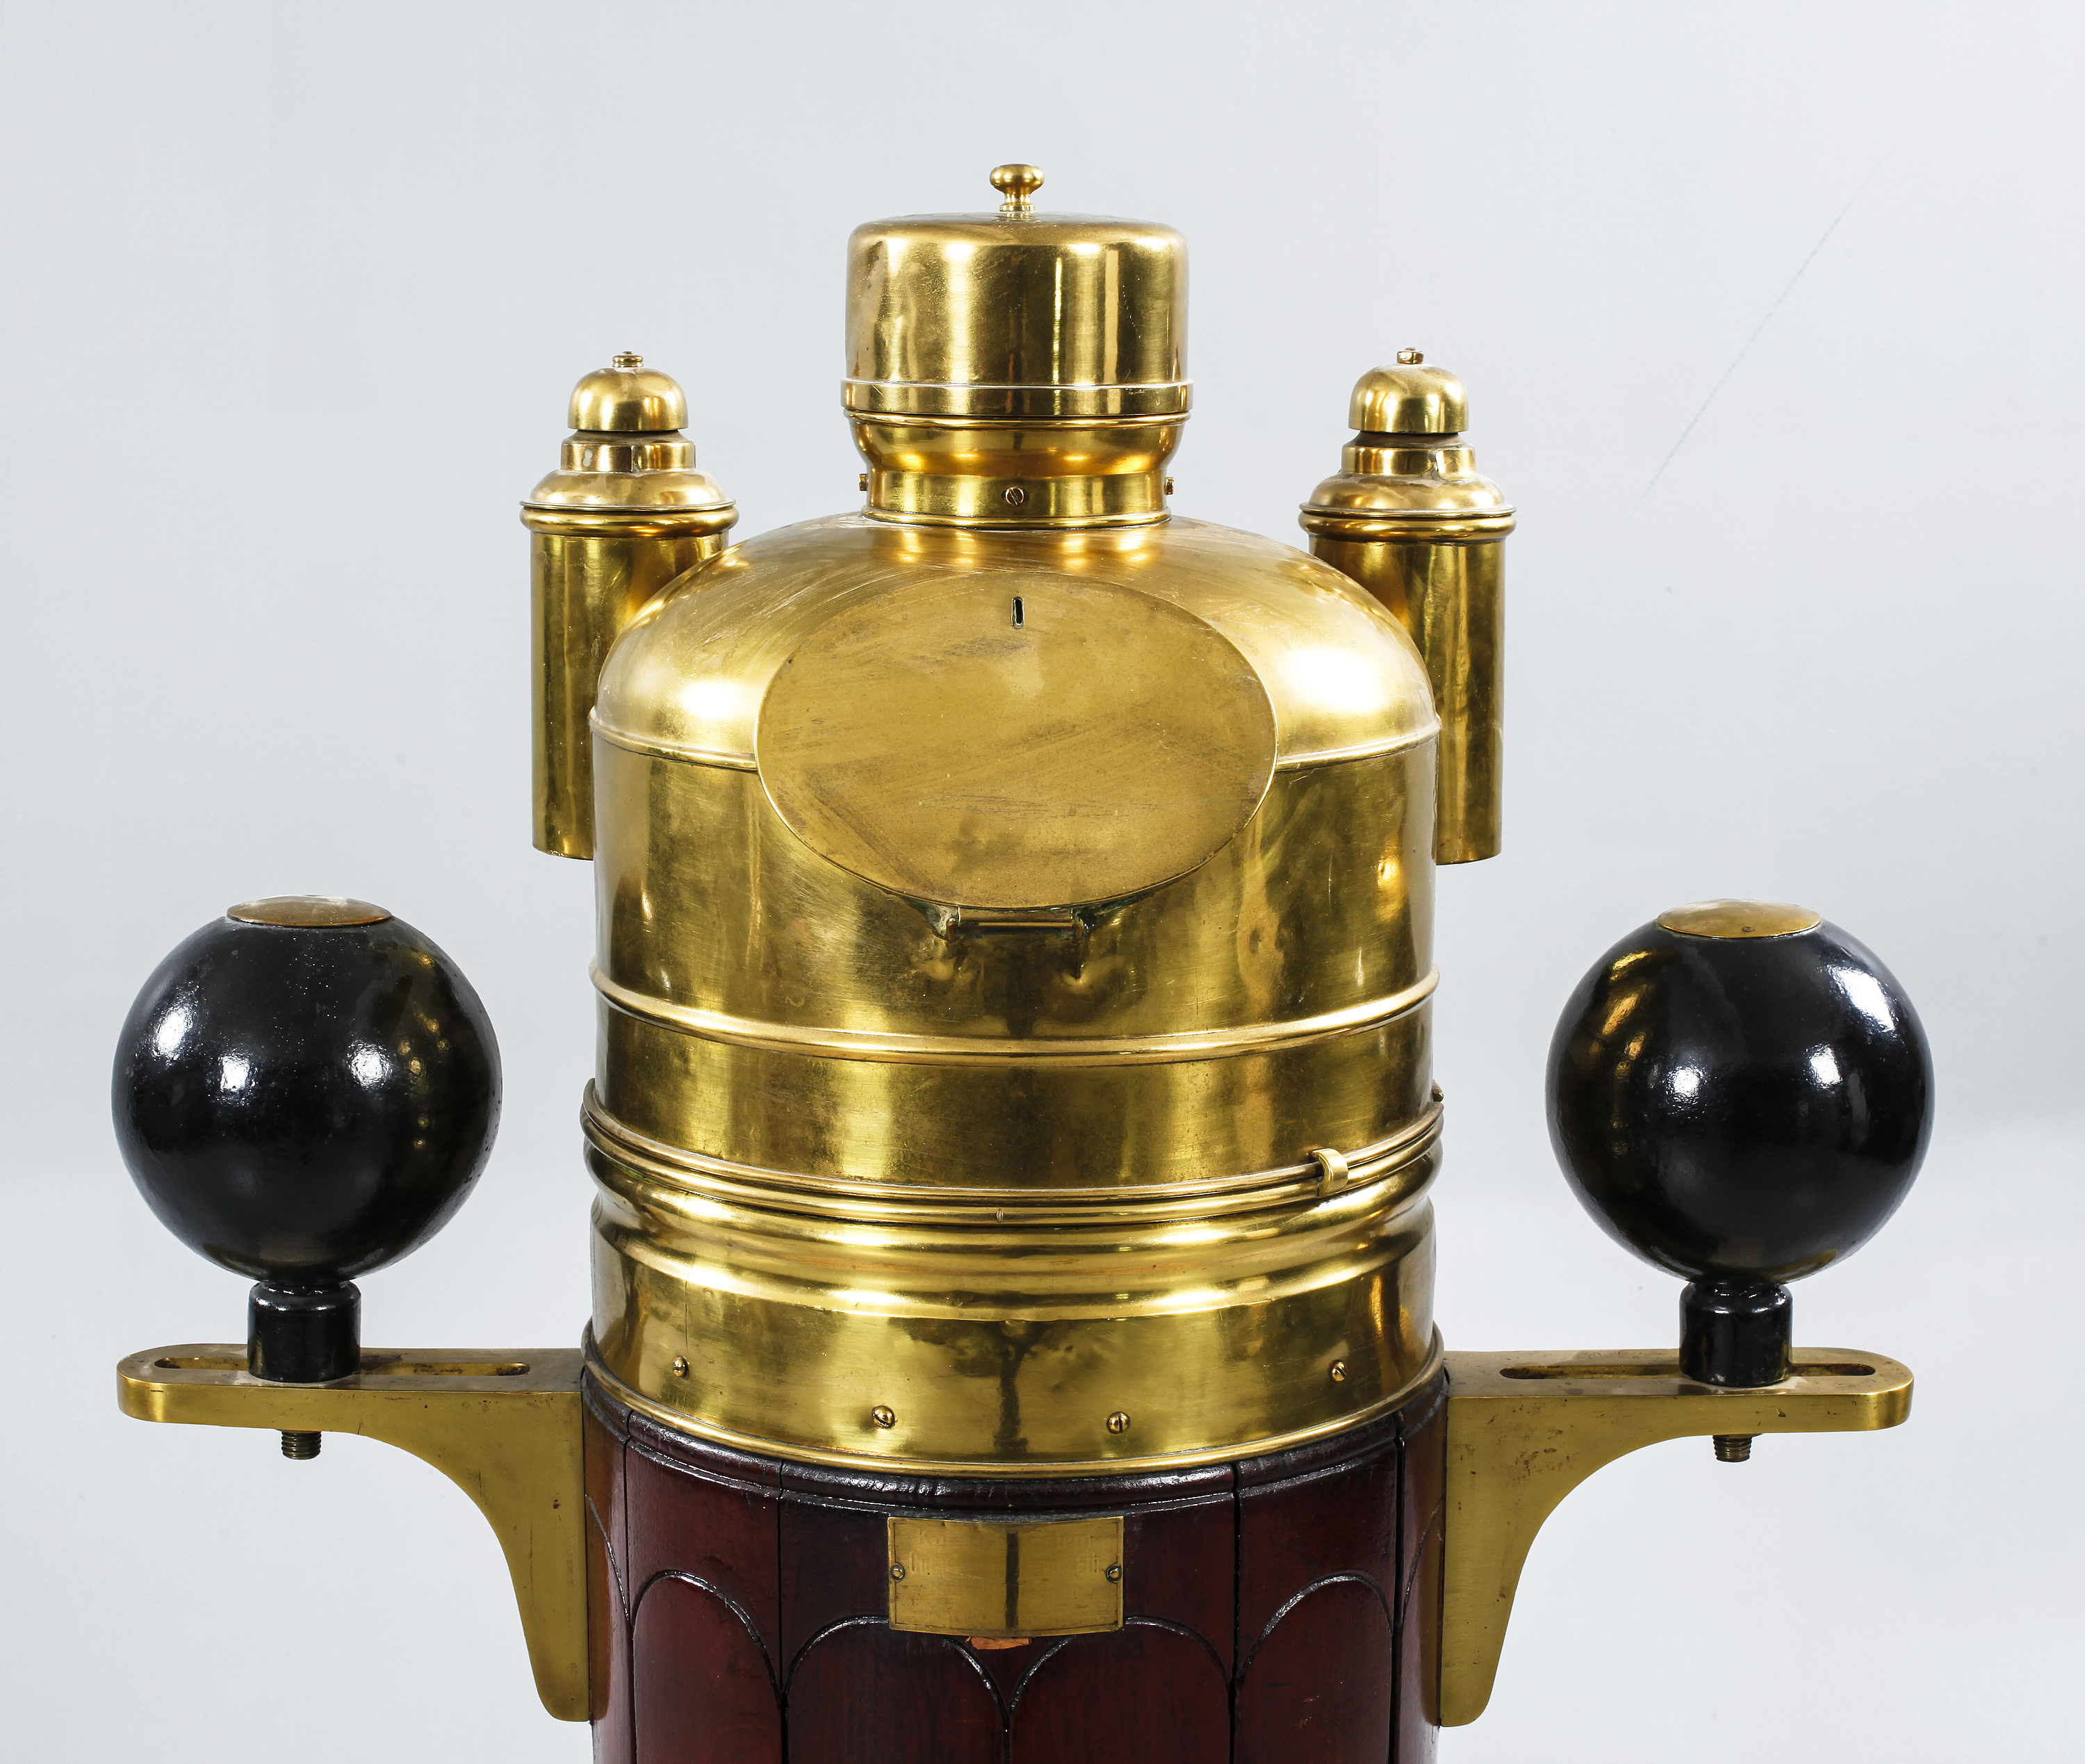
\includegraphics[scale=0.3]{Anh/ngoc2.jpg}
\end{center}

        Một hộp la bàn bảo vệ la bàn ở chính giữa, với hai quả cầu bằng sắt non để triệt tiêu phần bị lệch của la bàn, giúp la bàn quay đúng hướng. Việc sử dụng các quả cầu này được đề xuất bởi Lord Kelvin.

    Cũng như con tàu, các quả cầu sắt sẽ bị nhiễm từ do tác dụng của từ trường Trái Đất $B_e$. Là những quả cầu, chúng sẽ hoạt độn riên lẻ như các lưỡng cực. Một lưỡng cực có thể được coi như một trường tạo bởi hai đơn cực từ có moment từ $\pm m$ tại hai điểm khác nhau.
    Cảm ứng từ của một đơn cực từ là
    $$\ot{B}=\pm m\dfrac{\hat r}{r^2},$$
    Trong đó dấu dương tương ứng với cực bắc còn dấu âm tương ứng với cực nam. Từ trường của lưỡng cực là tổng hợp của hai trường: một của cực bắc tại $y=+a/2$ và một của cực nam tại $y=-a/2$, trong đó trục $y$ nằm ngang và hướng về phía bắc. $a$ là một khoảng cách nhỏ hơn rất nhiều so với bán kính các quả cầu; $a=K_iB_e$ trong đó $K_i$ là một hằng số phụ thuộc vào kích thước của các quả cầu sắt non.
    \begin{center}
        

\tikzset{every picture/.style={line width=0.75pt}} %set default line width to 0.75pt        

\begin{tikzpicture}[x=0.75pt,y=0.75pt,yscale=-1,xscale=1]
%uncomment if require: \path (0,466); %set diagram left start at 0, and has height of 466

%Shape: Circle [id:dp751806434667823] 
\draw   (98,277) .. controls (98,255.46) and (115.46,238) .. (137,238) .. controls (158.54,238) and (176,255.46) .. (176,277) .. controls (176,298.54) and (158.54,316) .. (137,316) .. controls (115.46,316) and (98,298.54) .. (98,277) -- cycle ;
%Straight Lines [id:da7958195415916756] 
\draw  [dash pattern={on 4.5pt off 4.5pt}]  (137,116) -- (137,284) ;
%Straight Lines [id:da11650011659130377] 
\draw  [dash pattern={on 4.5pt off 4.5pt}]  (137,277) -- (408,202) ;
%Straight Lines [id:da5651105007949573] 
\draw [line width=1.5]    (408,202) -- (466.27,224.56) ;
\draw [shift={(470,226)}, rotate = 201.16] [fill={rgb, 255:red, 0; green, 0; blue, 0 }  ][line width=0.08]  [draw opacity=0] (13.4,-6.43) -- (0,0) -- (13.4,6.44) -- (8.9,0) -- cycle    ;
%Shape: Circle [id:dp5068445005254147] 
\draw  [fill={rgb, 255:red, 0; green, 0; blue, 0 }  ,fill opacity=1 ] (132,262) .. controls (132,259.24) and (134.24,257) .. (137,257) .. controls (139.76,257) and (142,259.24) .. (142,262) .. controls (142,264.76) and (139.76,267) .. (137,267) .. controls (134.24,267) and (132,264.76) .. (132,262) -- cycle ;
%Shape: Circle [id:dp9877766218057484] 
\draw  [fill={rgb, 255:red, 0; green, 0; blue, 0 }  ,fill opacity=1 ] (132,289) .. controls (132,286.24) and (134.24,284) .. (137,284) .. controls (139.76,284) and (142,286.24) .. (142,289) .. controls (142,291.76) and (139.76,294) .. (137,294) .. controls (134.24,294) and (132,291.76) .. (132,289) -- cycle ;
%Straight Lines [id:da2796466001013038] 
\draw  [dash pattern={on 0.84pt off 2.51pt}]  (59,262) -- (137,262) ;
%Straight Lines [id:da8874709140465575] 
\draw  [dash pattern={on 0.84pt off 2.51pt}]  (59,289) -- (137,289) ;
%Straight Lines [id:da3482920020854341] 
\draw    (59,265) -- (59,289) ;
\draw [shift={(59,292)}, rotate = 270] [fill={rgb, 255:red, 0; green, 0; blue, 0 }  ][line width=0.08]  [draw opacity=0] (7.14,-3.43) -- (0,0) -- (7.14,3.43) -- (4.74,0) -- cycle    ;
\draw [shift={(59,262)}, rotate = 90] [fill={rgb, 255:red, 0; green, 0; blue, 0 }  ][line width=0.08]  [draw opacity=0] (7.14,-3.43) -- (0,0) -- (7.14,3.43) -- (4.74,0) -- cycle    ;

% Text Node
\draw (123,85.4) node [anchor=north west][inner sep=0.75pt]    {$\text{Bắc}$};
% Text Node
\draw (167,219.4) node [anchor=north west][inner sep=0.75pt]    {$\Phi $};
% Text Node
\draw (436,227.4) node [anchor=north west][inner sep=0.75pt]    {$\overrightarrow{B_{i}}$};
% Text Node
\draw (151,319.4) node [anchor=north west][inner sep=0.75pt]    {$\text{Bóng sắt}$};
% Text Node
\draw (37,267.4) node [anchor=north west][inner sep=0.75pt]    {$a$};


\end{tikzpicture}

    \end{center}
    \item Lập biểu thức cho từ trường $\ot{B_i}$ cách tâm quả cầu một khoảng $d\gg a$. Lưu ý rằng sẽ có một thành phần có phương hướng tâm, hướng ra quả cầu và một thành phần có phương tiếp tuyến với đường tròn bán kính $d$ xung quanh quả cầu, vì vậy nên sử dụng tọa độ cực.
    \item Nếu được đặt trực tiếp ở bên phải và trái của la bàn, các quả cầu sắt có thể được đặt ở khoảng cách $d$ để loại bỏ sai số từ tính cho các góc bất kì mà trong đó $\delta \theta$ là lớn nhất. Giả sử rằng điều này được thực hiện, tìm biểu thức cho góc lệch $\delta\theta$ do sự kết hợp hướng từ tính của con tàu và các quả cầu đối với góc $\theta$ bất kì.
\end{enumerate}

\end{vd}
\begin{loigiai}
\begin{enumerate}[1)]
    \item Phân tích từ trường tổng hợp thành các từ trường thành phần. Thành phần từ trường hướng về phía Bắc là:
$$B_{\text{bắc}}=B_e-B_eK_b\cos\theta\cos\theta-B_eK_s\sin\theta\sin\theta,$$
trong khi đó thành phần hướng về phía Đông là:
$$B_{\text{đông}}=-B_3K_b\sin\theta\cos\theta+B_eK_s\cos\theta\sin\theta.$$
Ta được góc lệch:
$$ \tan \delta \theta=\left(K_{s}-K_{b}\right) \dfrac{\sin \theta \cos \theta}{1-K_{b} \cos ^{2} \theta-K_{s} \sin ^{2} \theta}.$$
Dạng của biểu thức này khá đẹp, vì như ta thấy, $K_b$ và $K_s$ đủ nhỏ để có thể bỏ qua ở mẫu.
    \item Bằng cách kiểm tra, ta thấy $\theta=45^\circ$ sẽ ứng với góc lệch lớn nhất. Và ta chấp nhận được các góc $45^\circ$, $135^\circ$, $225^\circ$ và $315^\circ$.
    \item Bài toán này không khó như ta nghĩ.\\
    \begin{center}
        

\tikzset{every picture/.style={line width=0.75pt}} %set default line width to 0.75pt        

\begin{tikzpicture}[x=0.75pt,y=0.75pt,yscale=-1,xscale=1]
%uncomment if require: \path (0,468); %set diagram left start at 0, and has height of 468

%Shape: Circle [id:dp283743452851426] 
\draw   (118,297) .. controls (118,275.46) and (135.46,258) .. (157,258) .. controls (178.54,258) and (196,275.46) .. (196,297) .. controls (196,318.54) and (178.54,336) .. (157,336) .. controls (135.46,336) and (118,318.54) .. (118,297) -- cycle ;
%Straight Lines [id:da9329698416959988] 
\draw  [dash pattern={on 4.5pt off 4.5pt}]  (157,136) -- (157,304) ;
%Shape: Circle [id:dp7302446853963502] 
\draw  [fill={rgb, 255:red, 0; green, 0; blue, 0 }  ,fill opacity=1 ] (152,282) .. controls (152,279.24) and (154.24,277) .. (157,277) .. controls (159.76,277) and (162,279.24) .. (162,282) .. controls (162,284.76) and (159.76,287) .. (157,287) .. controls (154.24,287) and (152,284.76) .. (152,282) -- cycle ;
%Shape: Circle [id:dp08946091539998635] 
\draw  [fill={rgb, 255:red, 0; green, 0; blue, 0 }  ,fill opacity=1 ] (152,309) .. controls (152,306.24) and (154.24,304) .. (157,304) .. controls (159.76,304) and (162,306.24) .. (162,309) .. controls (162,311.76) and (159.76,314) .. (157,314) .. controls (154.24,314) and (152,311.76) .. (152,309) -- cycle ;
%Straight Lines [id:da8503315996944931] 
\draw  [dash pattern={on 0.84pt off 2.51pt}]  (79,282) -- (157,282) ;
%Straight Lines [id:da4363280092273607] 
\draw  [dash pattern={on 0.84pt off 2.51pt}]  (79,309) -- (157,309) ;
%Straight Lines [id:da08272405117413917] 
\draw    (79,285) -- (79,309) ;
\draw [shift={(79,312)}, rotate = 270] [fill={rgb, 255:red, 0; green, 0; blue, 0 }  ][line width=0.08]  [draw opacity=0] (7.14,-3.43) -- (0,0) -- (7.14,3.43) -- (4.74,0) -- cycle    ;
\draw [shift={(79,282)}, rotate = 90] [fill={rgb, 255:red, 0; green, 0; blue, 0 }  ][line width=0.08]  [draw opacity=0] (7.14,-3.43) -- (0,0) -- (7.14,3.43) -- (4.74,0) -- cycle    ;
%Straight Lines [id:da016285889610417215] 
\draw [color={rgb, 255:red, 0; green, 0; blue, 0 }  ,draw opacity=1 ]   (157,282) -- (389,243) ;
%Straight Lines [id:da05152532762538198] 
\draw    (170.5,305) -- (389,243) ;
%Straight Lines [id:da8507054364259559] 
\draw [color={rgb, 255:red, 245; green, 166; blue, 35 }  ,draw opacity=1 ]   (391.89,242.18) -- (498,212) ;
\draw [shift={(389,243)}, rotate = 344.12] [fill={rgb, 255:red, 245; green, 166; blue, 35 }  ,fill opacity=1 ][line width=0.08]  [draw opacity=0] (10.72,-5.15) -- (0,0) -- (10.72,5.15) -- (7.12,0) -- cycle    ;
%Straight Lines [id:da4895425189234859] 
\draw [color={rgb, 255:red, 74; green, 144; blue, 226 }  ,draw opacity=1 ][fill={rgb, 255:red, 74; green, 144; blue, 226 }  ,fill opacity=1 ]   (389,243) -- (500.05,223.52) ;
\draw [shift={(503,223)}, rotate = 530.05] [fill={rgb, 255:red, 74; green, 144; blue, 226 }  ,fill opacity=1 ][line width=0.08]  [draw opacity=0] (10.72,-5.15) -- (0,0) -- (10.72,5.15) -- (7.12,0) -- cycle    ;
%Straight Lines [id:da05906959057280403] 
\draw [color={rgb, 255:red, 208; green, 2; blue, 27 }  ,draw opacity=1 ]   (159.5,283.5) -- (170.5,305) ;
%Straight Lines [id:da6543050515321556] 
\draw [color={rgb, 255:red, 79; green, 211; blue, 33 }  ,draw opacity=1 ]   (157,309) -- (170.5,305) ;

% Text Node
\draw (143,105.4) node [anchor=north west][inner sep=0.75pt]    {$\text{Bắc}$};
% Text Node
\draw (187,239.4) node [anchor=north west][inner sep=0.75pt]    {$\Phi $};
% Text Node
\draw (57,287.4) node [anchor=north west][inner sep=0.75pt]    {$a$};


\end{tikzpicture}

    \end{center}
    Xét hình tam giác màu ở trên. Cạnh màu đen có chiều dài $a$. Góc giữa cạnh màu xanh và đen là $\Phi$, nên chiều dài cạnh đỏ là $a\sin \Phi$ và chiều dài cạnh xanh là $a\cos \Phi$.\\
    Cảm ứng từ gây ra bởi một cực từ cách một khoảng $d$ là
    $$B=\pm m\dfrac{1}{d^2}.$$
    Tổng hợp của hai trường gồm có hai thành phần. Thành phần tiếp tuyến được tính bằng độ mở của tam giác tạo bởi hai vector, và vì hai vector có chiều dài xấp xỉ nhau, nên chúng ta có thể dùng biểu thức của tam giác đồng dạng:
    $$\dfrac{a \sin \phi}{d} \approx \dfrac{B_{\phi}}{B} \Rightarrow B_{\phi}=m \dfrac{a}{d^{3}} \sin \phi=B_{e} \dfrac{m K_{i}}{d^{3}} \sin \phi .$$
    Như mong đợi, thành phần này biến mất vì $\Phi=0$.\\
    Thành phần theo phương bán kính được xác định bởi sự khác biệt chiều dài của hai vector của hai trường, là:
    $$ B_{r}=m\left(\dfrac{1}{d^{2}}-\dfrac{1}{(d+x)^{2}}\right)=\dfrac{m}{d^{2}}\left(1-\dfrac{1}{(1+x / d)^{2}}\right) \approx \dfrac{m}{d^{2}} \dfrac{2 x}{d},$$
    trong đó $x=a\cos\Phi$ là chiều dài cạnh xanh lá, vì thế
    $$B_r=2B_e\dfrac{mK_i}{d^3}\cos\Phi.$$
    \item Lưu ý rằng từ trường gần la bàn do hai viên bi sắt tạo ra hoạt động khá giống với từ trường do cả con tàu. Thành phần hướng về phía mũi tàu là:
    $$B_b=-2B_{\theta} \propto \sin\Phi\propto\cos\theta,$$
    và thành phần hướng về mạn phải là:
    $$B_s=2B_r \propto \cos\Phi\propto\sin\theta,$$
    trong đó có thừa số $2$ bởi vì có hai quả cầu. Lưu ý rằng $\theta$ là hướng đi của con tàu trong khi $\Phi$ là góc hợp bởi cực Bắc và vị trí của la bàn so với một trong các quả cầu. Do đó, nếu như từ trường được hiệu chỉnh sao cho các góc tối đa, nó sẽ loại bỏ từ trường do tàu gây ra cho tất cả các góc, hay
    $$\delta \theta=0,$$
    với mọi $\theta$. Điều này có nghĩa là ta sẽ đặt vị trí các quả cầu sao cho $K_b=K_s$.
\end{enumerate}
\end{loigiai}


\begin{vd}[Lưỡng cực từ quy mô hành tinh]
Từ trường của Trái Đất là gần giống với một từ trường của một lưỡng cực từ. Ta có thể tưởng tượng có một lưỡng cực từ $\ot{m}$ ở tâm của Trái Đất. Để đơn giản, giả sử rằng $\ot{m}$ nằm trên trục quay của Trái Đất, hướng từ Bắc vào Nam, như hình vẽ. Hồng Kông nằm ở vĩ độ $\alpha=22^\circ$. Từ trường tại điểm cách lưỡng cực từ một khoảng là $\ot{r}$ được tính theo công thức
\[\ot{B}=\dfrac{\mu_o}{4\pi}\left[\dfrac{3(\ot{m}\cdot\ot{r})\ot{r}}{r^3}-\dfrac{\ot{m}}{r^3}\right]\]
\begin{enumerate}[1) ]
    \item Tìm hướng của từ trường tại Hồng Kông theo các phía Đông, Tây, Bắc, Nam, và các góc hợp với mặt ngang.
    \item Một dây điện nằm ngang có chiều dài $10~\mathrm{m}$, mang dòng điện có cường độ $100~\mathrm{A}$ theo hướng Bắc $-$ Nam. Tìm lực từ tác dụng lên dây. (Bạn cần phải nhớ độ lớn của từ trường Trái Đất trên bề mặt Trái Đất).
\end{enumerate}
\begin{center}
    

\tikzset{every picture/.style={line width=0.75pt}} %set default line width to 0.75pt        

\begin{tikzpicture}[x=0.75pt,y=0.75pt,yscale=-1,xscale=1]
%uncomment if require: \path (0,300); %set diagram left start at 0, and has height of 300

%Shape: Circle [id:dp12955050763248477] 
\draw   (239,169) .. controls (239,124.26) and (275.26,88) .. (320,88) .. controls (364.74,88) and (401,124.26) .. (401,169) .. controls (401,213.74) and (364.74,250) .. (320,250) .. controls (275.26,250) and (239,213.74) .. (239,169) -- cycle ;
%Straight Lines [id:da33432597677839704] 
\draw  [dash pattern={on 0.84pt off 2.51pt}]  (208,170.33) -- (428,170.33) ;
%Straight Lines [id:da6659306133043119] 
\draw  [dash pattern={on 0.84pt off 2.51pt}]  (320,67.33) -- (320,270.33) ;
%Straight Lines [id:da013535855620636417] 
\draw    (320,169) -- (374.84,115.92) ;
\draw [shift={(377,113.83)}, rotate = 495.94] [fill={rgb, 255:red, 0; green, 0; blue, 0 }  ][line width=0.08]  [draw opacity=0] (10.72,-5.15) -- (0,0) -- (10.72,5.15) -- (7.12,0) -- cycle    ;
%Shape: Circle [id:dp570580867637053] 
\draw  [fill={rgb, 255:red, 0; green, 0; blue, 0 }  ,fill opacity=1 ] (379.5,113.83) .. controls (379.5,112.45) and (378.38,111.33) .. (377,111.33) .. controls (375.62,111.33) and (374.5,112.45) .. (374.5,113.83) .. controls (374.5,115.21) and (375.62,116.33) .. (377,116.33) .. controls (378.38,116.33) and (379.5,115.21) .. (379.5,113.83) -- cycle ;
%Straight Lines [id:da7218913590835949] 
\draw [line width=2.25]    (320,163.33) -- (320,177) ;
\draw [shift={(320,182)}, rotate = 270] [fill={rgb, 255:red, 0; green, 0; blue, 0 }  ][line width=0.08]  [draw opacity=0] (16.07,-7.72) -- (0,0) -- (16.07,7.72) -- (10.67,0) -- cycle    ;

% Text Node
\draw (338,124.4) node [anchor=north west][inner sep=0.75pt]    {$\ot{r}$};
% Text Node
\draw (296,175.4) node [anchor=north west][inner sep=0.75pt]    {$\ot{m}$};
% Text Node
\draw (342,149.4) node [anchor=north west][inner sep=0.75pt]    {$\alpha $};
% Text Node
\draw (387,97.4) node [anchor=north west][inner sep=0.75pt]    {$HK$};


\end{tikzpicture}
\end{center}
\end{vd}
\begin{loigiai}
\begin{enumerate}[1) ]
    \item 
    \begin{align*}
        \ot{B}&=\dfrac{\mu_0}{4\pi}\dfrac{1}{r^3}\left[3(\ot{m}\cdot\ot{r})\ot{r}-\ot{m}\right]\\
        &=\dfrac{\mu_0}{4\pi}\dfrac{1}{R^3}\left[3((-m\cdot\ot{z})\cdot\ot{r})\ot{r}-(-m)\ot{z}\right]\\
        &=\dfrac{\mu_0}{4\pi}\dfrac{m}{R^3}\left[-3\mathrm{\sin{\alpha}}\cdot\ot{r}+\left(\mathrm{\sin{\alpha}}\cdot\ot{r}-\mathrm{\cos{\alpha}}\cdot\ot{\theta}\right)\right]\\
        &=\dfrac{\mu_0}{4\pi}\dfrac{m}{R^3}\left[-2\mathrm{\sin{\alpha}}\cdot\ot{r}-\mathrm{\cos{\alpha}}\cdot\ot{\theta}\right].
    \end{align*}
    Từ Bắc tới Nam, tại góc $\beta=2\mathrm{\arctan{(2\mathrm{\tan{\alpha}})}}=38,9^\circ$ chỉ hướng xuống.
    \item $\left|\ot{B}\right|\cong0,5\cdot10^{-4}~\mathrm{T}$.
    Và độ lớn của lực từ là:
    \[\left|\ot{F}\right|=I\left|\ot{\ell}\times\ot{B}\right|=IB\ell\mathrm{\sin{\theta}}=0,0315~\mathrm{N}.\]
\end{enumerate}
\end{loigiai}

\begin{vd}[Dao động Plasma]
Một phiến kim loại có chiều dài $L$ và độ dày $h$, với $h\ll L$ (xem hình vẽ). Mật độ hạt dẫn electron và ion trong tấm lần lượt là $n_e$ và $n_i = n_e /Z$, với $Z$ là điện tích của các ion (điều này có nghĩa tổng điện tích của phiến bằng không).
\begin{center}


\tikzset{every picture/.style={line width=0.75pt}} %set default line width to 0.75pt        

\begin{tikzpicture}[x=0.75pt,y=0.75pt,yscale=-1,xscale=1]
%uncomment if require: \path (0,300); %set diagram left start at 0, and has height of 300

%Shape: Rectangle [id:dp7217887277897033] 
\draw  [draw opacity=0][fill={rgb, 255:red, 155; green, 155; blue, 155 }  ,fill opacity=0.6 ] (199,96) -- (279,96) -- (279,247) -- (199,247) -- cycle ;
%Shape: Rectangle [id:dp49084866599960386] 
\draw   (179,96) -- (257,96) -- (257,246.4) -- (179,246.4) -- cycle ;
%Straight Lines [id:da592262187480596] 
\draw    (165,102) -- (165,243) ;
\draw [shift={(165,246)}, rotate = 270] [fill={rgb, 255:red, 0; green, 0; blue, 0 }  ][line width=0.08]  [draw opacity=0] (10.72,-5.15) -- (0,0) -- (10.72,5.15) -- (7.12,0) -- cycle    ;
\draw [shift={(165,99)}, rotate = 90] [fill={rgb, 255:red, 0; green, 0; blue, 0 }  ][line width=0.08]  [draw opacity=0] (10.72,-5.15) -- (0,0) -- (10.72,5.15) -- (7.12,0) -- cycle    ;
%Straight Lines [id:da1395939334945815] 
\draw    (182,85) -- (253,85) ;
\draw [shift={(256,85)}, rotate = 180] [fill={rgb, 255:red, 0; green, 0; blue, 0 }  ][line width=0.08]  [draw opacity=0] (10.72,-5.15) -- (0,0) -- (10.72,5.15) -- (7.12,0) -- cycle    ;
\draw [shift={(179,85)}, rotate = 0] [fill={rgb, 255:red, 0; green, 0; blue, 0 }  ][line width=0.08]  [draw opacity=0] (10.72,-5.15) -- (0,0) -- (10.72,5.15) -- (7.12,0) -- cycle    ;
%Straight Lines [id:da6778726697290913] 
\draw    (259,253) -- (275,253) ;
\draw [shift={(278,253)}, rotate = 180] [fill={rgb, 255:red, 0; green, 0; blue, 0 }  ][line width=0.08]  [draw opacity=0] (10.72,-5.15) -- (0,0) -- (10.72,5.15) -- (7.12,0) -- cycle    ;


% Text Node
\draw (181,124.4) node [anchor=north west][inner sep=0.75pt]    {$+$};
% Text Node
\draw (181,166.4) node [anchor=north west][inner sep=0.75pt]    {$+$};
% Text Node
\draw (181,205.4) node [anchor=north west][inner sep=0.75pt]    {$+$};
% Text Node
\draw (264,123.4) node [anchor=north west][inner sep=0.75pt]    {$-$};
% Text Node
\draw (264,170.4) node [anchor=north west][inner sep=0.75pt]    {$-$};
% Text Node
\draw (264,206.4) node [anchor=north west][inner sep=0.75pt]    {$-$};
% Text Node
\draw (261,256.4) node [anchor=north west][inner sep=0.75pt]    {$\delta $};
% Text Node
\draw (152,165.4) node [anchor=north west][inner sep=0.75pt]    {$L$};
% Text Node
\draw (213,66.4) node [anchor=north west][inner sep=0.75pt]    {$h$};


\end{tikzpicture}
\end{center}
Bằng cách đặt tấm vào một điện trường đều bên ngoài, tất cả các electron đều bị dịch đi một khoảng nhỏ $\delta$, sao cho $|\delta| \ll h$, và vuông góc với trục của phiến. Chúng ta giả sử rằng $n_i$ và $n_e$ là không đổi, điện trường ngoài không làm nhiễu loạn mạng tinh thể và hiệu ứng rìa có thể được bỏ qua.
\begin{enumerate}[1)]
   \item Tính điện trường gây ra bởi sự dịch chuyển của các electron.
    \item Tính năng lượng điện trường của hệ.
Bây giờ điện trường ngoài bị tắt đi, và “mạng electron” bắt đầu dao động quanh vị trí cân bằng của nó.
  \item Tìm chu kì dao động của hệ với giả sử rằng độ dịch là nhỏ $(\delta \ll h)$.
\end{enumerate}
  
\end{vd}
\begin{loigiai}
  \begin{enumerate}[1)]
    \item Ta giả sử rằng $\delta >0$, sự dịch chuyển của các eletron dẫn điện do tác động của điện trường ngoài sẽ gây ra phân bố mật độ điện tích trên phiến.
\begin{center}


\tikzset{every picture/.style={line width=0.75pt}} %set default line width to 0.75pt        

\begin{tikzpicture}[x=0.75pt,y=0.75pt,yscale=-1,xscale=1]
%uncomment if require: \path (0,300); %set diagram left start at 0, and has height of 300

%Straight Lines [id:da6451691314240162] 
\draw    (78,141) -- (314.8,141) ;
\draw [shift={(317.8,141)}, rotate = 180] [fill={rgb, 255:red, 0; green, 0; blue, 0 }  ][line width=0.08]  [draw opacity=0] (10.72,-5.15) -- (0,0) -- (10.72,5.15) -- (7.12,0) -- cycle    ;
%Straight Lines [id:da1410092498727764] 
\draw    (100,257.9) -- (100,27.1) ;
\draw [shift={(100,24.1)}, rotate = 450] [fill={rgb, 255:red, 0; green, 0; blue, 0 }  ][line width=0.08]  [draw opacity=0] (10.72,-5.15) -- (0,0) -- (10.72,5.15) -- (7.12,0) -- cycle    ;
%Straight Lines [id:da15557261132056954] 
\draw [line width=1.5]    (100,60.2) -- (100,141) ;
%Straight Lines [id:da9142755166526642] 
\draw [line width=1.5]    (124.8,60.2) -- (124.8,141) ;
%Straight Lines [id:da4536569984572141] 
\draw [line width=1.5]    (234,141.2) -- (234,222) ;
%Straight Lines [id:da69833388035731] 
\draw [line width=1.5]    (258.8,141.2) -- (258.8,222) ;
%Straight Lines [id:da14094267922415105] 
\draw [line width=1.5]    (100,60.2) -- (125.8,60.2) ;
%Straight Lines [id:da3546021934992991] 
\draw [line width=1.5]    (233,222) -- (258.8,222) ;
%Straight Lines [id:da5560792612540038] 
\draw  [dash pattern={on 4.5pt off 4.5pt}]  (100.8,222) -- (233,222) ;


% Text Node
\draw (66,52.4) node [anchor=north west][inner sep=0.75pt]    {$+en$};
% Text Node
\draw (67,214.4) node [anchor=north west][inner sep=0.75pt]    {$-en$};
% Text Node
\draw (82,25.4) node [anchor=north west][inner sep=0.75pt]    {$\rho $};
% Text Node
\draw (294,143.4) node [anchor=north west][inner sep=0.75pt]    {$x$};
% Text Node
\draw (225,121.4) node [anchor=north west][inner sep=0.75pt]    {$h$};
% Text Node
\draw (245,121.4) node [anchor=north west][inner sep=0.75pt]    {$h+\delta $};
% Text Node
\draw (126.8,144.4) node [anchor=north west][inner sep=0.75pt]    {$\delta $};
% Text Node
\draw (84,143.4) node [anchor=north west][inner sep=0.75pt]    {$0$};


\end{tikzpicture}
\end{center}
      \[\varrho (x) = \left\{ \begin{array}{cc}
      0, & x<0, \\
     +en, & 0<x<\delta,\\
              0, &  \delta<x<h, \\
     -en, &h<x< h+\delta, \\
     0, & x> h+\delta. \end{array}\right. \tag{1}\]

Điện trường gây ra bởi phân bố này có thể được tính bằng cách kết hợp phương trình $\nabla \cdot \ot{E} = \partial_x E_x = 4\pi k_{\mathrm{e}} \varrho$ và điều kiện biên $\ot{E}(-\infty) =0$:
      \[E_x(x) = 4\pi e n k_{\mathrm{e}} \left\{ \begin{array}{cc} 
                       0, & x<0, \\
                 x, & 0<x<\delta, \\
                 \delta , & \delta<x<h,\\
                   h+ \delta - x, & h<x<h+\delta , \\
              0, & x>h+\delta . 
            \end{array}\right. \tag{2} \]

  \begin{center}


\tikzset{every picture/.style={line width=0.75pt}} %set default line width to 0.75pt        

\begin{tikzpicture}[x=0.75pt,y=0.75pt,yscale=-1,xscale=1]
%uncomment if require: \path (0,300); %set diagram left start at 0, and has height of 300

%Straight Lines [id:da01641255710506151] 
\draw    (98,161) -- (334.8,161) ;
\draw [shift={(337.8,161)}, rotate = 180] [fill={rgb, 255:red, 0; green, 0; blue, 0 }  ][line width=0.08]  [draw opacity=0] (10.72,-5.15) -- (0,0) -- (10.72,5.15) -- (7.12,0) -- cycle    ;
%Straight Lines [id:da14878370163317478] 
\draw    (120,185) -- (120,47.1) ;
\draw [shift={(120,44.1)}, rotate = 450] [fill={rgb, 255:red, 0; green, 0; blue, 0 }  ][line width=0.08]  [draw opacity=0] (10.72,-5.15) -- (0,0) -- (10.72,5.15) -- (7.12,0) -- cycle    ;
%Straight Lines [id:da8675826770429016] 
\draw [line width=0.75]  [dash pattern={on 4.5pt off 4.5pt}]  (120,88.2) -- (145.8,88.2) ;
%Straight Lines [id:da9262762168352314] 
\draw [line width=0.75]  [dash pattern={on 4.5pt off 4.5pt}]  (145.8,88.2) -- (145.8,160.6) ;
%Straight Lines [id:da7374057248217938] 
\draw [line width=0.75]  [dash pattern={on 4.5pt off 4.5pt}]  (233.8,88.2) -- (233.8,160.6) ;
%Straight Lines [id:da034445088923599654] 
\draw [line width=1.5]    (145.8,88.2) -- (120.6,160.6) ;
%Straight Lines [id:da6877283104927654] 
\draw [line width=1.5]    (145.8,88.2) -- (233.8,88.2) ;
%Straight Lines [id:da6022831934893127] 
\draw [line width=1.5]    (233.8,88.2) -- (260.8,160.6) ;


% Text Node
\draw (102,48.4) node [anchor=north west][inner sep=0.75pt]    {$E$};
% Text Node
\draw (90,78.4) node [anchor=north west][inner sep=0.75pt]    {$en\delta $};
% Text Node
\draw (107,162.4) node [anchor=north west][inner sep=0.75pt]    {$0$};
% Text Node
\draw (147.8,164) node [anchor=north west][inner sep=0.75pt]    {$\delta $};
% Text Node
\draw (224.9,164.4) node [anchor=north west][inner sep=0.75pt]    {$h$};
% Text Node
\draw (247,163.4) node [anchor=north west][inner sep=0.75pt]    {$h+\delta $};
% Text Node
\draw (312,164.4) node [anchor=north west][inner sep=0.75pt]    {$x$};


\end{tikzpicture}
\end{center}
Nếu chúng ta giả sử độ dịch là âm $-\delta$ (với $\delta>0$) thì mật độ điện tích và điện trường là 

    \[\begin{aligned}
       \varrho(x) &= 
       \left\{\begin{array}{cc}
                                     0, & x<-\delta,  \\
                              -en, & -\delta <x<0,\\
                            0, &  0<x<h-\delta, \\
                          +en, &h-\delta<x< h, \\
                               0,      &x> h . 
                  \end{array}\right.\\
        E_x(x) &= 4\pi e n k_{\mathrm{e}}   
        \left\{\begin{array}{cc}
                                     0, & x<-\delta,  \\
                              -en, & -\delta <x<0,\\
                            0, &  0<x<h-\delta, \\
                          +en, &h-\delta<x< h, \\
                               0,      &x> h . 
                  \end{array}\right. 
    \end{aligned}\tag{3}\]

Đồ thị cho trường hợp này có thể thu được bằng cách đảo trục $x$ và chuyển $\delta$ sang phần âm của trục $x$.
\item Năng lượng tĩnh điện của hệ, trong trường hợp độ dịch là dương, có thể tính được bằng tích phân mật độ năng lượng $u={E_x}^2/(8\pi k_{\mathrm{e}})$ trên toàn bộ vùng không gian:
 \[\begin{aligned}
U_{\mathrm{es}} &=\int \frac{E_{x}^{2}}{8 \pi k_{\mathrm{e}}} \mathrm{d}^{3} r=\frac{L^{2}}{8 \pi k_{\mathrm{e}}} \int_{0}^{h+\delta} E_{x}^{2} \mathrm{~d} x \\
&=\frac{L^{2}}{8 \pi k_{\mathrm{e}}}(4 \pi e n k_{\mathrm{e}})^{2}\left[\int_{0}^{\delta} x^{2} \mathrm{~d} x+\int_{\delta}^{h} \delta^{2} \mathrm{~d} x+\int_{h}^{h+\delta}(h+\delta-x)^{2} \mathrm{~d} x\right] \\
&=2 \pi k_{\mathrm{e}}(e n L)^{2}\left[\frac{\delta^{3}}{3}+\delta^{2}(h-\delta)+\frac{\delta^{3}}{3}\right]=2 \pi k_{\mathrm{e}}(e n L)^{2}\left(h \delta^{2}-\frac{\delta^{3}}{3}\right),
\end{aligned} \tag{4} \]
ở đây, do tính đối xứng của hệ, chúng ta sử dụng $\dd^3 r = L^2 \dd x $. Kết quả tương tự cũng sẽ đạt được nếu chúng ta coi độ dịch là $-\delta$. Độ dịch $\delta$ xuất hiện ở cuối biểu thức $4)$ trên thực tế phải được viết là $|\delta|$.
\item Ở giới hạn $\delta \ll h$ chúng ta có thể bỏ qua số hạng bậc ba của $\delta$ ở phương trình $4)$, và xấp xỉ $U_{\mathrm{es}} \approx 2\pi k_{\mathrm{e}} (enL)^2 h \delta^2$, năng lượng này là thế năng của một dao động điều hòa. Lực tác dụng lên ``mạng electron'' là 
   \[F= - \frac{\partial U_{\mathrm{es}}}{\partial \delta} = - 4 \pi k_{\mathrm{e}} (enL)^2h\delta, \tag{5}\]
ở đây $\delta$ có thể là âm hoặc dương. Phương trình chuyển động của electron là 
   \[M\ddot{\delta} = F = -M\omega^2\delta, \tag{6}\]
ở đây $M= m_e nL^2h$ là tổng khối lượng electron dẫn của bản. Từ đây ta có
     \[\omega^2 = \frac{4\pi k_{\mathrm{e}} n e^2}{m_e} \equiv \omega_p^2, \tag{7}\]
trong đó $\omega_p$ được gọi là tần số plasma, là một tính chất nội tại của vật dẫn, chỉ phụ thuộc vào mật độ electron tự do.
\end{enumerate}
\end{loigiai}


\begin{vd}[Cặp electrons và điện trường]
Ở đây chúng ta nghiên cứu chuyển động của hai electron trong mặt phẳng vuông góc với các đường sức của một từ trường đều. Hai electron được coi gần đúng như các chất điểm cổ điển và chỉ chịu tác dụng của lực điện và lực từ.
\begin{enumerate}[1)]
    \item Ban đầu hai electron đứng yên và cách nhau một khoảng là $d$. Chúng được truyền các vận tốc đầu cùng độ lớn $v$ nhưng ngược chiều nhau. Tìm điều kiện của $d$ để sau khi bắt đầu chuyển động, khoảng cách giữa chúng luôn là hằng số. Tìm biểu thức của $d$ lúc này.
    \item Chứng tỏ rằng có thể duy trì khoảng cách không đổi $d$ chỉ bằng cách truyền vận tốc cho một electron.Tìm quỹ đạo của khối tâm hệ trong trường hợp này. Vẽ phác họa quỹ đạo chuyển động của các electron. Khi nào thì electron ban đầu chuyển động sẽ dừng.
\end{enumerate}
\end{vd}
\begin{loigiai}
    \begin{enumerate}[1)]
        \item Để khoảng cách là không đổi, hai electron phải chuyển động cùng quỹ đạo trên cùng một đường tròn với bán kính $d/2$; chúng phải nằm đối xứng nhau qua tâm hình tròn và chuyển động với cùng vận tốc $v$ (như hình vẽ). Cả hai electron chuyển động trong từ trường đều chịu tác dụng của lực Lorentz và lực đẩy tĩnh điện giữa chúng tổng hợp lại thành một lực hướng tâm giữ cho chúng chuyển động thẳng đều.
        \begin{center}
            \tikzset{every picture/.style={line width=0.75pt}} %set default line width to 0.75pt        
            \begin{tikzpicture}[x=0.75pt,y=0.75pt,yscale=-1,xscale=1]
            %uncomment if require: \path (0,521); %set diagram left start at 0, and has height of 521
            
            %Shape: Ellipse [id:dp37933654197498545] 
            \draw   (166.08,212.4) .. controls (166.08,156.95) and (211.03,112) .. (266.48,112) .. controls (321.93,112) and (366.88,156.95) .. (366.88,212.4) .. controls (366.88,267.85) and (321.93,312.8) .. (266.48,312.8) .. controls (211.03,312.8) and (166.08,267.85) .. (166.08,212.4) -- cycle ;
            %Shape: Ellipse [id:dp020176206185545054] 
            \draw  [fill={rgb, 255:red, 0; green, 0; blue, 0 }  ,fill opacity=1 ] (161.72,212.4) .. controls (161.72,209.99) and (163.67,208.03) .. (166.08,208.03) .. controls (168.49,208.03) and (170.45,209.99) .. (170.45,212.4) .. controls (170.45,214.81) and (168.49,216.77) .. (166.08,216.77) .. controls (163.67,216.77) and (161.72,214.81) .. (161.72,212.4) -- cycle ;
            %Shape: Ellipse [id:dp7333140222111905] 
            \draw  [fill={rgb, 255:red, 0; green, 0; blue, 0 }  ,fill opacity=1 ] (362.52,212.4) .. controls (362.52,209.99) and (364.47,208.03) .. (366.88,208.03) .. controls (369.29,208.03) and (371.25,209.99) .. (371.25,212.4) .. controls (371.25,214.81) and (369.29,216.77) .. (366.88,216.77) .. controls (364.47,216.77) and (362.52,214.81) .. (362.52,212.4) -- cycle ;
            %Straight Lines [id:da5858758890164644] 
            \draw    (166.08,208.03) -- (166.08,165.68) ;
            \draw [shift={(166.08,163.68)}, rotate = 450] [color={rgb, 255:red, 0; green, 0; blue, 0 }  ][line width=0.75]    (10.93,-3.29) .. controls (6.95,-1.4) and (3.31,-0.3) .. (0,0) .. controls (3.31,0.3) and (6.95,1.4) .. (10.93,3.29)   ;
            %Straight Lines [id:da6699826148149972] 
            \draw    (166.08,212.4) -- (226.94,212.4) ;
            \draw [shift={(228.94,212.4)}, rotate = 180] [color={rgb, 255:red, 0; green, 0; blue, 0 }  ][line width=0.75]    (10.93,-3.29) .. controls (6.95,-1.4) and (3.31,-0.3) .. (0,0) .. controls (3.31,0.3) and (6.95,1.4) .. (10.93,3.29)   ;
            %Straight Lines [id:da12871600619765244] 
            \draw    (367.75,212.4) -- (399.8,212.4) ;
            \draw [shift={(401.8,212.4)}, rotate = 180] [color={rgb, 255:red, 0; green, 0; blue, 0 }  ][line width=0.75]    (10.93,-3.29) .. controls (6.95,-1.4) and (3.31,-0.3) .. (0,0) .. controls (3.31,0.3) and (6.95,1.4) .. (10.93,3.29)   ;
            %Straight Lines [id:da33537398216713554] 
            \draw    (366.88,212.4) -- (308.64,212.4) ;
            \draw [shift={(306.64,212.4)}, rotate = 360] [color={rgb, 255:red, 0; green, 0; blue, 0 }  ][line width=0.75]    (10.93,-3.29) .. controls (6.95,-1.4) and (3.31,-0.3) .. (0,0) .. controls (3.31,0.3) and (6.95,1.4) .. (10.93,3.29)   ;
            %Straight Lines [id:da39133811789746975] 
            \draw    (166.08,212.4) -- (133.16,212.4) ;
            \draw [shift={(131.16,212.4)}, rotate = 360] [color={rgb, 255:red, 0; green, 0; blue, 0 }  ][line width=0.75]    (10.93,-3.29) .. controls (6.95,-1.4) and (3.31,-0.3) .. (0,0) .. controls (3.31,0.3) and (6.95,1.4) .. (10.93,3.29)   ;
            %Straight Lines [id:da8153194046125287] 
            \draw    (366.88,212.4) -- (366.88,265.58) ;
            \draw [shift={(366.88,267.58)}, rotate = 270] [color={rgb, 255:red, 0; green, 0; blue, 0 }  ][line width=0.75]    (10.93,-3.29) .. controls (6.95,-1.4) and (3.31,-0.3) .. (0,0) .. controls (3.31,0.3) and (6.95,1.4) .. (10.93,3.29)   ;
            %Straight Lines [id:da11308212969163933] 
            \draw    (266.48,212.4) -- (305.31,299.8) ;
            \draw [shift={(306.12,301.63)}, rotate = 246.05] [color={rgb, 255:red, 0; green, 0; blue, 0 }  ][line width=0.75]    (10.93,-3.29) .. controls (6.95,-1.4) and (3.31,-0.3) .. (0,0) .. controls (3.31,0.3) and (6.95,1.4) .. (10.93,3.29)   ;
            %Shape: Circle [id:dp5670320230480146] 
            \draw   (224.58,170.06) .. controls (224.58,165.38) and (228.37,161.59) .. (233.04,161.59) .. controls (237.72,161.59) and (241.51,165.38) .. (241.51,170.06) .. controls (241.51,174.73) and (237.72,178.53) .. (233.04,178.53) .. controls (228.37,178.53) and (224.58,174.73) .. (224.58,170.06) -- cycle ;
            %Straight Lines [id:da8344401093990392] 
            \draw [line width=1.5]    (228.69,166.45) -- (237.02,174.78) ;
            %Straight Lines [id:da8741424678522312] 
            \draw [line width=1.5]    (237.02,166.45) -- (228.61,174.86) ;
            
            
            
            % Text Node
            \draw (242.96,146.8) node [anchor=north west][inner sep=0.75pt]    {$\ot{B}$};
            % Text Node
            \draw (152.16,169.01) node [anchor=north west][inner sep=0.75pt]    {$v$};
            % Text Node
            \draw (367.8,241.99) node [anchor=north west][inner sep=0.75pt]    {$v$};
            % Text Node
            \draw (186.64,192.45) node [anchor=north west][inner sep=0.75pt]    {$F_{L}$};
            % Text Node
            \draw (328.94,192.45) node [anchor=north west][inner sep=0.75pt]    {$F_{L}$};
            % Text Node
            \draw (136.37,191.58) node [anchor=north west][inner sep=0.75pt]    {$F_{C}{}_{b}$};
            % Text Node
            \draw (370.34,190.7) node [anchor=north west][inner sep=0.75pt]    {$F_{C}{}_{b}$};
            % Text Node
            \draw (290.04,227.85) node [anchor=north west][inner sep=0.75pt]    {$\dfrac{d}{2}$};
            \end{tikzpicture}
        \end{center}
    Chúng ta viết phương trình chuyển động cho một electron. Lực lorentz tác dụng lên một hạt với điện tích $-e$, khối lượng $m$ và vận tốc $v$ là 
    \[F_L=evB,\]
    và lực đẩy Coulomb giữa hai electron \[F_{Cb}=k_{\mathrm{e}}\dfrac{e^2}{d^2}.\]
    Lực Coulomb luôn là lực đẩy và vì lực Lorentz luôn vuông góc với vận tốc nên cả hai lực này đều theo phương xuyên tâm so với quỹ đạo của hạt. 
    \\ \textbf{Chú ý:} Trên lí thuyết chúng ta phải tính thêm cả lực từ do từ trường của electron chuyển động gây ra (và có thể tính được thông qua định lí Biot-Savart):
         \[F_{\mathrm{magn}}=e v \frac{\mu_{0}}{4 \pi} \frac{e v}{d^{2}}=\frac{v^{2}}{c^{2}} F_{\mathrm{Cb}},\]
    trong đó $c$ là vận tốc ánh sáng trong chân không. Tuy nhiên trong giới hạn của cơ học cổ điển phi tương đối tính, $v\ll c$, lực này là không đáng kể so với lực Coulomb. Do đó chúng ta bỏ qua lực này.
    Phương trình chuyển động của electron do đó là
        \[evB-k_{\mathrm{e}}\dfrac{e^2}{d^2}=m\dfrac{v^2}{d/2}.\]
    Đây là một phương trình bậc hai của $v$, và các nghiệm của nó là
        \[v=\dfrac{edB}{4m} \pm \sqrt{\left(\dfrac{edB}{4m}\right)^2-\dfrac{k_{\mathrm{e}}e^2}{2md}}.\]
    Điều kiện để bài có thể thỏa mãn nếu như vận tốc thu được là số thực và dương, do đó biểu thức trong căn phải là dương. Do đó ta thu được điều kiện của $d$ là 
        \[d \geqslant 2\sqrt[3]{{\frac{{{k_{\mathrm{e}}}m}}{{{B^2}}}}} = {d_{\mathrm{crit}}}.\]
    Nếu các electron gần nhau hơn khoảng cách giới hạn, chúng ta sẽ không tìm được nghiệm. Nếu khoảng cách đúng bằng khoảng cách giới hạn, ta thu được nghiệm duy nhất. Còn nếu khoảng cách lớn hơn $d_{crit}$, chúng ta luôn thu được hai nghiệm vận tốc thỏa mãn. 
    
      \item Nếu chỉ một electron được cung cấp vận tốc đầu, chuyển động sẽ trở nên phức tạp hơn, kể cả đối với trường hợp đặc biệt của đề bài, đó là khoảng cách của 2 electron là không đổi. \\
   Chúng ta có thể tiếp cận gần hơn với lời giải khi xử lí được câu hỏi phụ trợ ``quỹ đạo của khối tâm hệ lúc này như nào?'' \\
   Dùng các phương trình vector cơ bản của chuyển động ta có:
   \[m \ot{a_1} = k_{\mathrm{e}} \dfrac{e^{2}}{\left|\ot{r_1}- \ot{r_2}\right|^{3}}\left(\ot{r_1}-\ot{r_2}\right)-e \ot{v_1} \times \ot{B}, \tag{1}\label{N.5.1}\]
    \[m \ot{a_2} = k_{\mathrm{e}} \dfrac{e^{2}}{\left|\ot{r_1}-\ot{r_2}\right|^{3}}\left(\ot{r_2}-\ot{r_1}\right)-e \ot{v_2} \times \ot{B}. \tag{2}\label{N.5.2} \]
    Với hai hạt có cùng khối lượng, chúng ta có thể công nhận
    \[\ot{r_{\mathrm{CM}}}=\frac{\ot{r_1}+\ot{r_2}}{2}, \quad \ot{v_{\mathrm{CM}}}=\dfrac{\ot{v_1}+\ot{v_2}}{2}, \quad \ot{a_{\mathrm{CM}}}=\dfrac{\ot{a_1}+\ot{a_2}}{2}.\]
     Và phương trình chuyển động tổng quát của cả hai hạt
     \[m\left(\ot{a_1}+\ot{a_2}\right) = 0-e\left(\ot{v_1}+\ot{v_2}\right) \times \ot{B},\]
     Từ đó, ta dẫn ra 
     \[m \ot{a_\mathrm{CM}}=-e \ot{v_\mathrm{CM}} \times \ot{B}.\]
      Đối với hệ khối tâm, tương tác Coulomb nội tại đã được triệt tiêu.\\
    Phương trình cuối cùng là tiền đề để ta kết luận rằng khối tâm của hệ hai electron chuyển động trong từ trường tương tự như một electron duy nhất. Nếu từ trường là đều và chuyển động vuông góc với các đường sức từ, thì khối tâm của hệ chuyển động với quỹ đạo tròn đều!\\
    Chúng ta kết luận rằng khối tâm chuyển động tròn đều, còn hai electron ``dao động'' quanh quỹ đạo đó. Vận tốc góc của khối tâm là:
    \[\omega_{\mathrm{CM}}=\dfrac{a_{\mathrm{CM}}}{v_{\mathrm{CM}}}=\dfrac{e}{m} B=\omega_{\mathrm{c}}.\]
    Kết quả này cũng giống tần số cyclotron của electron $-$ vận tốc góc của các electron trong các máy gia tốc hạt. Bán kính của quỹ đạo khối tâm là
    \[R_{\mathrm{CM}}=\dfrac{v_{\mathrm{CM}}}{\omega_{\mathrm{CM}}}=\dfrac{v_{\mathrm{CM}}}{\omega_{\mathrm{c}}}.\]
    Thế các electron chuyển động xung quanh khối tâm như nào? Lời giải cho câu hỏi này cũng chính là đáp số cuối cùng của bài toán. Chúng ta viết vector độ dời của electron $1$ là $\ot{r_1} =\ot{r_\mathrm{CM}}+\ot{R}$. Do đó vector độ dời của electron 2 là $\ot{r_2} = \ot{r_\mathrm{CM}} - \ot{R}$. Dùng định nghĩa khối tâm ta có
    \[\ot{R}=\ot{r_1}-\ot{r_\mathrm{CM}}=\ot{r_1}-\dfrac{\ot{r_1}+\ot{r_2}}{2}=\dfrac{\ot{r_1}-\ot{r_2}}{2}.\]
     Một phương trình về sự thay đổi của vector này theo thời gian có thể được dẫn ra từ sự khác biệt giữa phương trình (\ref{N.5.1}) và (\ref{N.5.2})
     \[m\left(\ot{a_1}-\ot{a_2}\right)=2 k_{\mathrm{e}} \dfrac{e^{2}}{\left|\ot{r_1}-\ot{r_2}\right|^{3}}\left(\ot{r_1}-\ot{r_2}\right)-e\left[\left(\ot{v_1}-\ot{v_2}\right) \times \ot{B}\right].\tag{3}\label{N.5.3}\]
     Sự khác biệt của hai vector độ dời chính là $2$ lần vector $\ot R$ ở trên; do đó sự khác biệt về vận tốc chính là $2$ lần vector $\ot V$ (độ thay đổi của vector $\ot R$ theo thời gian). Và suy luận tương tự cũng được áp dụng với gia tốc.
     \[\ot{r_1} - \ot{r_2} =2 \ot{R}, \quad \ot{v_1}-\ot{v_2}=2 \ot{V}, \quad \ot{a_1}-\ot{a_2}=2 \ot{A}.\]
    Dùng bổ chính này, phương trình (\ref{N.5.3}) có thể được viết lại thành:
    \[m \ot{A}=k_{\mathrm{e}} \dfrac{e^{2}}{\left|2 \ot{R}\right|^{3}} 2 \ot{R} - e \tron{\ot{V} \times \ot{B}}. \tag{4}\label{N.5.4}\]
     Phương trình chuyển động này nội tại tương tự với phương trình ở câu $1)$, khi mà khối tâm của hệ đứng yên, do đó phương trình này cũng có nghiệm là chuyển động tròn đều.\\
   Công nhận dạng nghiệm của phương trình, nếu độ lớn của vector $\ot{R}(t)$ không thay đổi theo thời gian với giá trị $R$, và hướng của nó quay với vận tốc góc $\omega$, áp dụng phương trình của chuyển động tròn đều, ta có
    \[A=-\omega^{2} R \ {\text { và }} \  \ot{V} \times \ot{B}=R \omega B.\]
    Và từ phương trình (\ref{N.5.4}), chúng ta thu được phương trình bậc hai cho vận tốc góc $\omega$ của cặp electron, khi chúng quay quanh khối tâm:
    \[\omega^{2}-\dfrac{e}{m} B \omega + \dfrac{k_{\mathrm{e}}}{m} \dfrac{e^{2}}{4 R^{3}}=0. \tag{5}\label{N.5.5}\]
    Nghiệm thực của phương trình xuất hiện khi biểu thức $\Delta$ không âm, tức là
    \[R \geq \sqrt[3]{\dfrac{k_{\mathrm{e}} m}{B^{2}}}.\] 
      Lúc này khoảng cách tối thiểu giữa hai electron là 
      \[d_{\min }=2 R_{\min }=2 \sqrt[3]{\dfrac{k_{\mathrm{e}} m}{B^{2}}}=d_{\text{crit}}.\]
    Tất cả các lập luận của chúng ta đều thỏa mãn kể cả khi khối tâm của hệ không chuyển động, do đó không có gì bất ngờ khi giá trị của $d_{\mathrm{crit}}$ là giống hệt trong phần $1)$.\\
     Chúng ta sẽ phác họa quỹ đạo của hai electron trong trường hợp $d = d_{\min}$, khi đó
     \[R=R_{\min}=\sqrt[3]{\dfrac{k_{\mathrm{e} } m}{B^{2}}}.\]
     
     Thay giá trị này vào phương trình (\ref{N.5.5}), ta thu được vận tốc góc của hai electron chuyển động quanh khối tâm
    \[\omega = \dfrac{1}{2} \dfrac{e}{m} B=\dfrac{1}{2} \omega_{\mathrm{c}}.\]
    Giá trị của vận tốc góc này đúng bằng một nửa giá trị vận tốc góc của khối tâm.\\
   Kích thích hệ, như mô tả của ý $2)$, một electron được cấp vận tốc ban đầu $v_0$. Vận tốc này phải vuông góc với đường nối tâm của hai electron, nếu không khoảng cách giữa chúng sẽ thay đổi ngay tức thì sau đó.\\
   Ban đầu electron thứ $2$ sẽ ở trạng thái đứng yên và khối tâm chuyển động với vận tốc $v_0/2$, do đó vận tốc của mỗi electron đối với khối tâm có độ lớn bằng nhau nhưng ngược hướng.\\
   Với chuyển động tròn quanh khối tâm, ta có 
    \[\dfrac{v_0}{2} = R\omega = R \dfrac{\omega_{\mathrm{c}}}{2}.\]
    Đồng thời, với chuyển động tròn của khối tâm, ta có
    \[\dfrac{v_{0}}{2} = R_{\mathrm{CM}} \omega_{\mathrm{c}}, \ \text{ nên }  \ R_{\mathrm{CM}}=\dfrac{R}{2}.\]
     Do đó, electron chuyển động tròn quanh khối tâm với một quỹ đạo có bán kính gấp đôi bán kính chuyển động tròn của khối tâm. Hơn nữa chu kì quay của khối tâm bằng một nửa chu kì của electron quay quanh nó.\\
     Hình vẽ phác họa của quỹ đạo electron như trên hình $2$. Để dễ hình dung hơn, chúng ta thêm vào cả quỹ đạo của khối tâm electron (được vẽ bằng các nét đứt). Khi đường nối electron quay được một góc $\theta$ quanh khối tâm thì khối tâm đã quay được một góc $2 \theta$ trên quỹ đạo riêng của nó, với bán kính quỹ đạo bằng một nửa.

    \begin{center}
        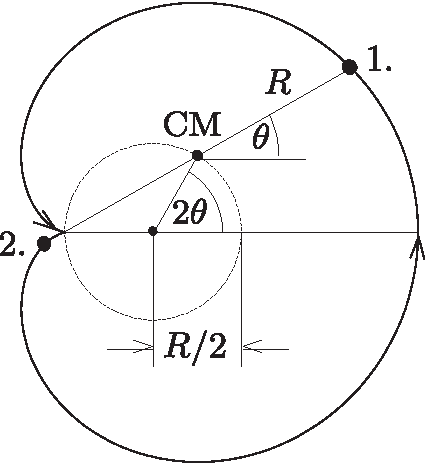
\includegraphics[scale=0.75]{Anh/Nam4.pdf}\\
        Hình $2$.
    \end{center}
     Sau một chu kì $T = \dfrac{2\pi}{\omega_{\mathrm{c}}}$, khối tâm hoàn thành một vòng quay của nó, nhưng mỗi electron chỉ đi được nửa vòng; và do đó chúng đổi vị trí cho nhau. Tại thời điểm đó, vị trí và vận tốc của khối tâm giống hệt như lúc bắt đầu chuyển động $(v_0/2)$, electron ban đầu đứng yên có vận tốc $v_0$ và electron được kích thích bây giờ đứng yên. Nó dừng lại lần đầu tiên sau 
     \[T = 2\pi \dfrac{m}{eB}.\]
    \textbf{Mở rộng:}
    \begin{enumerate}[1)]
        \item Quỹ đạo chuyển động của hai eletron (được gọi là đường cardioid hay đường “trái tim”, do hình dạng đặc biệt của nó) chỉ đơn giản và đơn điệu chỉ khi khoảng cách ban đầu giữa các $e$ bằng khoảng cách giới hạn với từ trường cho trước. Nếu khoảng cách giữa chúng lớn hơn khoảng cách giới hạn, lúc đó quỹ đạo và chuyển động của các electron không đơn giản nữa, và nhìn chung quỹ đạo lúc này sẽ là quỹ đạo mở (điểm bắt đầu và kết thúc chu kì không trùng nhau).
        \item Bài toán sẽ càng phức tạp nếu vận tốc ban đầu không thỏa mãn điều kiện khoảng cách không đổi. Nhưng kể cả khi đó ta có thể chứng minh rằng hai electron không thể tiến tới quá gần nhau cũng như rời quá xa nhau, do đó khoảng cách giữa chúng sẽ dao động giữa hai giá trị giới hạn.
    \end{enumerate}
        
    \end{enumerate}
\end{loigiai}


\begin{vd}[Anode và Cathode] %VPhO 2018
Một linh kiện điện tử có cấu tạo gồm một cathode $K$ dạng sợi dây dẫn mảnh, thẳng, dài và một anode $A$ dạng trụ rỗng, có bán kính ${R}$, bao quanh cathode và có trục trùng với cathode. Linh kiện đặt trong không gian có từ trường đều $\ot{B}$ hướng dọc theo cathode. Bằng một cách nào đó, người ta tạo một điện trường $\ot{E}$ hướng trục từ ${A}$ đến ${K}$ có độ lớn không đổi.\\
Do tính đối xứng trục của bài toán, ta xét một hệ tọa độ trụ như hình. Hệ tọa độ được chọn sao cho gốc ${O}$ nằm trên ${K}$, trục ${Oz}$ theo chiều $\ot{B}$, từ trường $\ot{B}=\left(B_{\rho}, B_{\theta}, B_{z}\right)=(0,0, B)$
và điện trường
$$\ot{E}=\left(E_{\rho}, E_{\theta}, E_{z}\right)=(E, 0,0).$$ 
Khi cathode ${K}$ được đốt nóng sẽ bức xạ electron. Coi vận tốc của các electron phát ra từ cathode ${K}$ là rất nhỏ và bỏ qua tác dụng của trọng lực lên các electron này. Khi xem xét chuyển động của electron, không gian trong linh kiện có thể coi là chân không.
\begin{center}
{
\tikzset{every picture/.style={line width=0.75pt}} %set default line width to 0.75pt        

\begin{tikzpicture}[x=0.75pt,y=0.75pt,yscale=-1,xscale=1]
%uncomment if require: \path (0,474); %set diagram left start at 0, and has height of 474

%Shape: Ellipse [id:dp991714530186085] 
\draw   (223.14,115.72) .. controls (223.14,102.67) and (263.03,92.09) .. (312.24,92.09) .. controls (361.45,92.09) and (401.34,102.67) .. (401.34,115.72) .. controls (401.34,128.77) and (361.45,139.35) .. (312.24,139.35) .. controls (263.03,139.35) and (223.14,128.77) .. (223.14,115.72) -- cycle ;
%Straight Lines [id:da5090442830728876] 
\draw    (223.14,115.72) -- (223.14,275.3) ;
%Curve Lines [id:da8521350306505784] 
\draw  [dash pattern={on 4.5pt off 4.5pt}]  (223.55,208.65) .. controls (232.86,175.87) and (389.76,176.83) .. (401.75,208.65) ;
%Curve Lines [id:da6280284607936966] 
\draw    (223.55,208.65) .. controls (229.55,236.18) and (387.07,242.39) .. (401.75,208.65) ;
%Curve Lines [id:da06707199242837247] 
\draw  [dash pattern={on 4.5pt off 4.5pt}]  (223.14,275.3) .. controls (232.44,242.52) and (389.35,243.47) .. (401.34,275.3) ;
%Curve Lines [id:da3349004032829275] 
\draw    (223.14,275.3) .. controls (229.14,302.83) and (386.66,309.04) .. (401.34,275.3) ;
%Straight Lines [id:da40853559092842495] 
\draw    (401.34,115.72) -- (401.34,275.3) ;
%Straight Lines [id:da6012789690231846] 
\draw  [dash pattern={on 4.5pt off 4.5pt}]  (223.55,208.65) -- (401.75,208.65) ;
%Straight Lines [id:da565528652758621] 
\draw    (401.75,208.65) -- (456.22,208.65) ;
\draw [shift={(459.22,208.65)}, rotate = 180] [fill={rgb, 255:red, 0; green, 0; blue, 0 }  ][line width=0.08]  [draw opacity=0] (10.72,-5.15) -- (0,0) -- (10.72,5.15) -- (7.12,0) -- cycle    ;
%Straight Lines [id:da9860459074898706] 
\draw  [dash pattern={on 4.5pt off 4.5pt}]  (312.65,115.72) -- (312.65,273.71) ;
%Straight Lines [id:da37175075777238975] 
\draw    (312.65,79.49) -- (312.65,115.72) ;
\draw [shift={(312.65,76.49)}, rotate = 90] [fill={rgb, 255:red, 0; green, 0; blue, 0 }  ][line width=0.08]  [draw opacity=0] (10.72,-5.15) -- (0,0) -- (10.72,5.15) -- (7.12,0) -- cycle    ;
%Straight Lines [id:da6837228115665901] 
\draw  [dash pattern={on 4.5pt off 4.5pt}]  (312.65,208.65) -- (262.68,227.29) ;
%Straight Lines [id:da5422064545392717] 
\draw    (262.68,227.29) -- (206.97,245.77) ;
\draw [shift={(204.12,246.71)}, rotate = 341.65] [fill={rgb, 255:red, 0; green, 0; blue, 0 }  ][line width=0.08]  [draw opacity=0] (10.72,-5.15) -- (0,0) -- (10.72,5.15) -- (7.12,0) -- cycle    ;
%Straight Lines [id:da17772674300232527] 
\draw  [dash pattern={on 4.5pt off 4.5pt}]  (311.62,273.71) -- (401.34,273.71) ;
%Straight Lines [id:da7646362348207041] 
\draw  [dash pattern={on 4.5pt off 4.5pt}]  (311.62,273.71) -- (254.7,292.49) ;
%Straight Lines [id:da9590432766813448] 
\draw  [dash pattern={on 4.5pt off 4.5pt}]  (312.65,208.65) -- (355.03,222.47) ;
%Straight Lines [id:da5777038896986804] 
\draw  [dash pattern={on 4.5pt off 4.5pt}]  (312.65,153.91) -- (355.03,167.73) ;
%Straight Lines [id:da5586061217127374] 
\draw  [dash pattern={on 4.5pt off 4.5pt}]  (355.03,167.73) -- (355.03,222.47) ;
%Straight Lines [id:da9883977422064121] 
\draw [color={rgb, 255:red, 74; green, 144; blue, 226 }  ,draw opacity=1 ]   (312.65,208.65) -- (352.87,169.81) ;
\draw [shift={(355.03,167.73)}, rotate = 496] [fill={rgb, 255:red, 74; green, 144; blue, 226 }  ,fill opacity=1 ][line width=0.08]  [draw opacity=0] (10.72,-5.15) -- (0,0) -- (10.72,5.15) -- (7.12,0) -- cycle    ;
%Shape: Arc [id:dp20863658466452928] 
\draw  [draw opacity=0] (321.86,213.17) .. controls (320.24,215.56) and (317.19,217.33) .. (313.45,217.73) .. controls (308.96,218.21) and (304.72,216.57) .. (302.44,213.81) -- (311.91,209.17) -- cycle ; \draw   (321.86,213.17) .. controls (320.24,215.56) and (317.19,217.33) .. (313.45,217.73) .. controls (308.96,218.21) and (304.72,216.57) .. (302.44,213.81) ;

% Text Node
\draw (470.17,201.29) node [anchor=north west][inner sep=0.75pt]    {$y$};
% Text Node
\draw (322.16,66.24) node [anchor=north west][inner sep=0.75pt]    {$z$};
% Text Node
\draw (296.52,143.26) node [anchor=north west][inner sep=0.75pt]    {$z$};
% Text Node
\draw (189.03,234.18) node [anchor=north west][inner sep=0.75pt]    {$x$};
% Text Node
\draw (269.77,263.67) node [anchor=north west][inner sep=0.75pt]    {$R$};
% Text Node
\draw (316.9,256.99) node [anchor=north west][inner sep=0.75pt]    {$K$};
% Text Node
\draw (362.57,150.9) node [anchor=north west][inner sep=0.75pt]    {$M$};
% Text Node
\draw (406.86,267.17) node [anchor=north west][inner sep=0.75pt]    {$A$};
% Text Node
\draw (296.15,215.37) node [anchor=north west][inner sep=0.75pt]    {$\theta $};
% Text Node
\draw (329.6,211.82) node [anchor=north west][inner sep=0.75pt]    {$\rho $};
\end{tikzpicture}
}\end{center}
Kí hiệu điện tích nguyên tố là $e$ và khối lượng electron là $m_{e}$. Giả sử ở thời điểm $t=0$ electron có tọa độ $\left(0,0, z_{0}\right)$, ở thời điểm $t>0$ electron ở tọa độ $(\rho, \theta, z)$, hãy:
\begin{enumerate}[1)]
    \item Viết các phương trình vi phân mô tả chuyển động của electron.
    \item Tìm phương trình quỹ đạo của electron.
    \item Tìm vận tốc dài của electron tại thời điểm $t$ bất kì.
\end{enumerate}
Cho biết trong hệ tọa độ trụ:
\begin{itemize}
    \item Chất điểm $M$ xác định bởi vector tọa độ $\overrightarrow{OM} = (\rho, \theta, z)$ có vận tốc và gia tốc tương ứng là $\ot{v}=(\dot{\rho}, \rho \dot{\theta}, \dot{z})$ và $\ot{a}=\left(\ddot{\rho}-\rho \dot{\theta}^{2}, \dfrac{1}{\rho} \dfrac{\dd}{\dd t}\left(\rho^{2} \dot{\theta}\right), \ddot{z}\right)$.
    \item Nếu $\ot{a}=\left(a_{\rho}, a_{\theta}, a_{z}\right), \ot{b}=\left(b_{\rho}, b_{\theta}, b_{z}\right)$ thì $$\ot{a}\times\ot{b}=\left(a_{\theta} b_{z}-a_{z} b_{\theta}, a_{z} b_{\rho}-a_{\rho} b_{z}, a_{\rho} b_{\theta}-a_{\theta} b_{\rho}\right)$$
\end{itemize}
\end{vd}
\begin{loigiai}
\begin{enumerate}[1)]
    \item 
Áp dụng định luật II Newton cho electron
\[-e\ot{E} - e \ot{v} \times \ot{B} = m_e \ot{a}.\]
Trong hệ tọa độ trụ, phương trình được viết lại như sau
\[-e\tron{E,0,0} - e \tron{\dot{\rho}, \rho \dot{\theta}, \dot{z}} \times \tron{0,0,B} = m_e \left(\ddot{\rho}-\rho \dot{\theta}^{2}, \dfrac{1}{\rho} \dfrac{\dd}{\dd t}\left(\rho^{2} \dot{\theta}\right), \ddot{z}\right).\]
\[\rt \tron{-\dfrac{eE + eB\rho \dot{\theta}}{m_e}, \dfrac{eB\dot{\rho}}{m_e}, 0} = \left(\ddot{\rho}-\rho \dot{\theta}^{2}, \dfrac{1}{\rho} \dfrac{\dd}{\dd t}\left(\rho^{2} \dot{\theta}\right), \ddot{z}\right).\]
Vậy ta có hệ phương trình vi phân mô tả chuyển động của các electron:
\begin{subnumcases}{}
 -\ddot{\rho} + \rho \dot{\theta}^{2} &= $\dfrac{eE + eB\rho \dot{\theta}}{m_e}$ \label{q.vp.2.1a}\\ 
\dfrac{\dd}{\dd t}\left(\rho^{2} \dot{\theta}\right) &=  $\dfrac{eB\rho\dot{\rho}}{m_e}$ \label{q.vp.2.1b}\\ 
\ddot{z} &= $0$ \label{q.vp.2.1c}
\end{subnumcases}
\item 
Từ phương trình (\ref{q.vp.2.1c}) và điều kiện đầu $t = 0$, $\heva{z &= z_0 \\ v_z &= 0}$, ta suy ra
\[v_z = 0 \rt z = z_0. \tag{2}\label{q.vp.2.2}\]
Nhân hai vế của phương trình (\ref{q.vp.2.1b}) cho $\dd t$, ta được
\[\dd \left(\rho^{2} \dot{\theta}\right) = \dfrac{eB}{m_e}\rho \dd \rho.\]
Lấy nguyên hàm hai vế
\[\dfrac{eB}{2m_e} \rho^2 = \rho^2 \dot{\theta} + C.\]
Từ điều kiện đầu: khi $t = 0$, $\rho = 0$ suy ra được hằng số $C = 0$. Thay vào phương trình trên ta suy ra
\[\dot{\theta } = \dfrac{eB}{2m_e} = \mathrm{const} \rt \theta = \dfrac{eB}{2m_e} t. \tag{3}\label{q.vp.2.3}\]
Thay (\ref{q.vp.2.3}) vào (\ref{q.vp.2.1a}), ta được
\[\ddot{\rho} + \tron{\dfrac{eB}{2m_e}}^2 \rho + \dfrac{eE}{m_e} = 0.\]
Nghiệm của phương trình này có dạng
\[\rho = A\cos\left(\dfrac{eB}{2m_e} t + \varphi\right) - \dfrac{eE}{m_e}.\]
Tại $t = 0$, $\heva{\rho &= 0 \\ \dot{\rho} &= 0} \rt \heva{A \cos \varphi - \dfrac{eE}{m_e} &= 0 \\ -A\dfrac{eB}{2m_e}\sin \varphi &= 0} \rt \heva{A &= \dfrac{eE}{m_e} \\ \varphi &= 0}$. \\
Thay vào phương trình trên, ta được
\[\rho = \dfrac{eE}{m_e} \tron{\cos \dfrac{eB}{2m_e} t - 1}. \tag{4}\label{q.vp.2.4}\]
Từ (\ref{q.vp.2.2}), (\ref{q.vp.2.3}) và (\ref{q.vp.2.4}), ta suy ra phương trình quỹ đạo của electron:
\[\heva{\rho &= \dfrac{eE}{m_e} \tron{\cos \theta - 1} \\ z &= z_0}.\]
\item Vận tốc của electron tại thời điểm $t$ được tính bởi:
\[\ot{v}=(\dot{\rho}, \rho \dot{\theta}, \dot{z}) = \tron{-\dfrac{e^2EB}{2m_e^2}\sin \dfrac{eB}{2m_e}t, \dfrac{e^2EB}{2m_e^2} \tron{\cos \dfrac{eB}{2m_e} t - 1}, 0}.\]
\[\rt v = \dfrac{e^2EB}{m_e^2} \sqrt{2 - 2\cos \dfrac{eB}{2m_e} t} = \dfrac{e^2EB}{m_e^2} \sin \dfrac{eB}{4m_e} t.\]
\end{enumerate}
\end{loigiai}



\begin{vd}[Cảm ứng Faraday]
Theo định luật cảm ứng điện từ Faraday, khi từ thông qua một vòng dây biến đổi, trong vòng dây sẽ xuất hiện một suất điện động cảm ứng ${V}$ có độ lớn tỷ lệ thuận với tốc độ biến thiên từ thông. Chiều của suất điện động này tuân theo quy tắc Lenz, tức là dòng cảm ứng sẽ chống lại sự biến thiên của từ thông. Tổng quát mà nói, khi từ trường biến thiên theo thời gian thì trong không gian sẽ xuất hiện điện trường cảm ứng, bất kể có vòng dây ở đó hay không. Sử dụng định luật này có thể giải được nhiều bài toán. Nhưng trước hết hãy xem xét mối liên hệ toán học giữa điện trường cảm ứng và từ trường biến thiên theo thời gian.\\
Trên một đường cong khép kín ${C}$, ta quy ước một chiều dương như hình ${a})$. Một mặt ${S}$ được giới hạn bởi đường cong kín ${C}$, từ thông gửi qua mặt ${S}$ ký hiệu bởi $\Phi({S})$. Từ thông qua mặt sẽ nhận dấu dương nếu khi nắm tay phải quay theo chiều của đường cong ${C}$ thì nó tiến về trước. Trong trường hợp diện tích phẳng $A$ thì từ thông không phụ thuộc vào vị trí của mặt $S$. Khi từ trường $\ot{B}$ vuông góc với mặt ${S}$ thì từ thông cho bởi: $\Phi({S}) = {BA}$.
\begin{center}


\tikzset{every picture/.style={line width=0.75pt}} %set default line width to 0.75pt        

\begin{tikzpicture}[x=0.75pt,y=0.75pt,yscale=-1,xscale=1]
%uncomment if require: \path (0,456); %set diagram left start at 0, and has height of 456

%Right Arrow [id:dp20646986306348958] 
\draw   (238.83,233.3) -- (179.21,135.59) -- (169.82,141.32) -- (164.5,90.35) -- (207.38,118.4) -- (197.99,124.13) -- (257.61,221.84) -- cycle ;
%Shape: Ellipse [id:dp6912657668631246] 
\draw   (168.07,209.37) .. controls (154.19,191.64) and (164.51,160.38) .. (191.11,139.56) .. controls (217.71,118.75) and (250.52,116.24) .. (264.4,133.97) .. controls (278.27,151.7) and (267.96,182.95) .. (241.36,203.77) .. controls (214.76,224.59) and (181.95,227.1) .. (168.07,209.37) -- cycle ;
%Curve Lines [id:da5271502020531298] 
\draw    (213.33,234.11) .. controls (259.33,217.38) and (272.74,198.77) .. (283.8,175.35) ;
\draw [shift={(285,172.78)}, rotate = 474.7] [fill={rgb, 255:red, 0; green, 0; blue, 0 }  ][line width=0.08]  [draw opacity=0] (10.72,-5.15) -- (0,0) -- (10.72,5.15) -- (7.12,0) -- cycle    ;
%Shape: Polygon [id:ds8845684539905239] 
\draw   (445.29,113.5) -- (500.73,171.77) -- (497.9,213.64) -- (419.26,232.49) -- (374,184.41) -- (390.97,136.88) -- cycle ;
%Straight Lines [id:da7470426544470834] 
\draw    (404.17,154.14) -- (422.62,86.22) ;
\draw [shift={(423.41,83.32)}, rotate = 465.2] [fill={rgb, 255:red, 0; green, 0; blue, 0 }  ][line width=0.08]  [draw opacity=0] (10.72,-5.15) -- (0,0) -- (10.72,5.15) -- (7.12,0) -- cycle    ;
%Curve Lines [id:da7884871002948666] 
\draw    (418.88,187.8) .. controls (394.92,156.04) and (429.14,123.17) .. (453.96,166.53) ;
\draw [shift={(455.09,168.56)}, rotate = 241.78] [fill={rgb, 255:red, 0; green, 0; blue, 0 }  ][line width=0.08]  [draw opacity=0] (10.72,-5.15) -- (0,0) -- (10.72,5.15) -- (7.12,0) -- cycle    ;
%Shape: Arc [id:dp18207070073520004] 
\draw  [draw opacity=0] (415.9,112.28) .. controls (418.41,112.76) and (420.75,114.15) .. (422.37,116.38) .. controls (423.75,118.27) and (424.4,120.47) .. (424.37,122.64) -- (413.96,122.51) -- cycle ; \draw   (415.9,112.28) .. controls (418.41,112.76) and (420.75,114.15) .. (422.37,116.38) .. controls (423.75,118.27) and (424.4,120.47) .. (424.37,122.64) ;

% Text Node
\draw (104.17,191.5) node [anchor=north west][inner sep=0.75pt]   [align=left] {Đường\\cong $C$};
% Text Node
\draw (125.67,67) node [anchor=north west][inner sep=0.75pt]   [align=left] {Từ thông $ \Phi $};
% Text Node
\draw (213.17,252.9) node [anchor=north west][inner sep=0.75pt]    {$a)$};
% Text Node
\draw (221.5,146.35) node [anchor=north west][inner sep=0.75pt]   [align=left] {Mặt $ S$};
% Text Node
\draw (288,153) node [anchor=north west][inner sep=0.75pt]   [align=left] {Chiều\\dương};
% Text Node
\draw (402.7,72.44) node [anchor=north west][inner sep=0.75pt]    {$\ot{E}$};
% Text Node
\draw (378.94,117.87) node [anchor=north west][inner sep=0.75pt]    {$P$};
% Text Node
\draw (445.89,93.55) node [anchor=north west][inner sep=0.75pt]    {$Q$};
% Text Node
\draw (423.07,99.61) node [anchor=north west][inner sep=0.75pt]    {$\theta $};
% Text Node
\draw (432.53,176.18) node [anchor=north west][inner sep=0.75pt]   [align=left] {Chiều\\dương};
% Text Node
\draw (509.67,209.13) node [anchor=north west][inner sep=0.75pt]   [align=left] {Đường\\cong $C$};
% Text Node
\draw (433.45,252.62) node [anchor=north west][inner sep=0.75pt]    {$b)$};
\end{tikzpicture}
\end{center}
Ta tưởng tượng một vòng dây dẫn đặt đúng theo đường cong $C$, một suất điện động cảm ứng ${V}({C})$ sẽ xuất hiện trong khung dây. Đường cong kín đó có thể là đa giác giống như trong hình $b)$. Khi giữa hai đầu ${P}, {Q}$ của dây dẫn xuất hiện một suất điện động $V(\ot{PQ})$, trên đoạn thẳng ${PQ}$ xuất hiện một điện trường $\ot{E}$ hướng từ ${P}$ về ${Q}$. Góc giữa phương của điện trường và $\overrightarrow{PQ}$ là $\theta$, chiều dài đoạn thẳng là $l_{PQ}$.
\[V(\ot{PQ}) = |E| l_{PQ} \cos \theta = E_{C} l_{P Q}.\]
Ở đây, $|E|$ là độ lớn của điện trường, $E_{c}=|E| \cos \theta$ là thành phần của điện trường lên phương của đường cong ${C}$. Nếu tính suất điện động cảm ứng trên từng đoạn của đường cong ${C}$ rồi cộng tất cả vào với nhau, ta sẽ tìm được suất điện động cảm ứng trên cả đường cong ${C}$. Trường hợp đặc biệt khi đường cong ${C}$ đặt trùng với đường sức điện trường có độ lớn $|E|$ không đổi, thì tại mọi điểm của đường cong ${C}$ ta có $E_{C} = |E|$ hoặc $-|E|$. Nếu chiều dài tổng cộng của đường cong ${C}$ là $l$, thì ${V}({C}) = E_{c} l$.\\
Giả sử có một từ trường biến thiên theo thời gian, khi đó dọc theo đường cong $C$ sẽ xuất hiện một điện trường. Từ thông gửi qua mặt ${S}$ biến thiên theo thời gian nên suất điện động cảm ứng ở mép của mặt ${S}$ có thể được viết:
\[
{V}({C})=\dfrac{\Delta \Phi(S)}{\Delta t}.
\tag{1}\label{q.d.1}\]
Đây chính là định luật cảm ứng điện từ Faraday mà ta đã đề cập từ đầu.\\

\textbf{Chú ý.} Trên thực tế thì các đường sức điện cảm ứng sẽ bị nhiễu động do ảnh hưởng của hiện tượng phân cực điện khi ta đưa dây dẫn vào bên trong điện trường. Nhưng ta chỉ quan tâm đến quan hệ giữa điện trường và từ trường trong trường hợp không bị ảnh hưởng bởi dây dẫn. Trong khi tính suất điện động ${V}({C})$ dọc theo đường cong kín và điện trường ta bỏ qua ảnh hưởng của dây dẫn.
    \begin{center}
\tikzset{every picture/.style={line width=0.75pt}} %set default line width to 0.75pt        

\begin{tikzpicture}[x=0.75pt,y=0.75pt,yscale=-1,xscale=1]
%uncomment if require: \path (0,508); %set diagram left start at 0, and has height of 508

%Curve Lines [id:da17704119093765347] 
\draw    (265.22,236.28) .. controls (262.37,135.31) and (215.55,95.15) .. (188.73,88.59) ;
\draw [shift={(185.9,88.01)}, rotate = 369.33000000000004] [fill={rgb, 255:red, 0; green, 0; blue, 0 }  ][line width=0.08]  [draw opacity=0] (10.72,-5.15) -- (0,0) -- (10.72,5.15) -- (7.12,0) -- cycle    ;
%Shape: Rectangle [id:dp2836649028479259] 
\draw  [line width=1.5]  (47.59,118.54) -- (132.66,118.54) -- (132.66,205.43) -- (47.59,205.43) -- cycle ;
\draw  [fill={rgb, 255:red, 0; green, 0; blue, 0 }  ,fill opacity=1 ] (88.13,114.41) -- (96.8,118.75) -- (88.13,123.08) -- (92.46,118.75) -- cycle ;
\draw  [fill={rgb, 255:red, 0; green, 0; blue, 0 }  ,fill opacity=1 ] (136.96,155.39) -- (132.63,164.06) -- (128.29,155.39) -- (132.63,159.73) -- cycle ;
\draw  [fill={rgb, 255:red, 0; green, 0; blue, 0 }  ,fill opacity=1 ] (93.71,209.74) -- (85.04,205.41) -- (93.71,201.07) -- (89.37,205.41) -- cycle ;
\draw  [fill={rgb, 255:red, 0; green, 0; blue, 0 }  ,fill opacity=1 ] (43.33,162.14) -- (47.66,153.47) -- (52,162.14) -- (47.66,157.81) -- cycle ;
%Straight Lines [id:da7848944881489814] 
\draw    (39.64,236.71) -- (39.64,89.18) ;
\draw [shift={(39.64,86.18)}, rotate = 450] [fill={rgb, 255:red, 0; green, 0; blue, 0 }  ][line width=0.08]  [draw opacity=0] (10.72,-5.15) -- (0,0) -- (10.72,5.15) -- (7.12,0) -- cycle    ;
%Straight Lines [id:da7900679033699884] 
\draw    (52.55,236.71) -- (52.55,89.18) ;
\draw [shift={(52.55,86.18)}, rotate = 450] [fill={rgb, 255:red, 0; green, 0; blue, 0 }  ][line width=0.08]  [draw opacity=0] (10.72,-5.15) -- (0,0) -- (10.72,5.15) -- (7.12,0) -- cycle    ;
%Straight Lines [id:da8748247138522687] 
\draw    (66.46,236.71) -- (66.46,89.18) ;
\draw [shift={(66.46,86.18)}, rotate = 450] [fill={rgb, 255:red, 0; green, 0; blue, 0 }  ][line width=0.08]  [draw opacity=0] (10.72,-5.15) -- (0,0) -- (10.72,5.15) -- (7.12,0) -- cycle    ;
%Straight Lines [id:da14628756799680054] 
\draw    (83.34,236.71) -- (83.34,89.18) ;
\draw [shift={(83.34,86.18)}, rotate = 450] [fill={rgb, 255:red, 0; green, 0; blue, 0 }  ][line width=0.08]  [draw opacity=0] (10.72,-5.15) -- (0,0) -- (10.72,5.15) -- (7.12,0) -- cycle    ;
%Straight Lines [id:da7920165637776044] 
\draw    (102.2,236.71) -- (102.2,89.18) ;
\draw [shift={(102.2,86.18)}, rotate = 450] [fill={rgb, 255:red, 0; green, 0; blue, 0 }  ][line width=0.08]  [draw opacity=0] (10.72,-5.15) -- (0,0) -- (10.72,5.15) -- (7.12,0) -- cycle    ;
%Straight Lines [id:da7403220227482121] 
\draw    (123.06,236.71) -- (123.06,89.18) ;
\draw [shift={(123.06,86.18)}, rotate = 450] [fill={rgb, 255:red, 0; green, 0; blue, 0 }  ][line width=0.08]  [draw opacity=0] (10.72,-5.15) -- (0,0) -- (10.72,5.15) -- (7.12,0) -- cycle    ;
%Straight Lines [id:da018032475368297662] 
\draw    (147.88,236.71) -- (147.88,89.18) ;
\draw [shift={(147.88,86.18)}, rotate = 450] [fill={rgb, 255:red, 0; green, 0; blue, 0 }  ][line width=0.08]  [draw opacity=0] (10.72,-5.15) -- (0,0) -- (10.72,5.15) -- (7.12,0) -- cycle    ;
%Curve Lines [id:da2082178622856372] 
\draw    (255.84,236.82) .. controls (249.84,143.51) and (213.08,115.42) .. (189.79,107.29) ;
\draw [shift={(186.95,106.38)}, rotate = 376.5] [fill={rgb, 255:red, 0; green, 0; blue, 0 }  ][line width=0.08]  [draw opacity=0] (10.72,-5.15) -- (0,0) -- (10.72,5.15) -- (7.12,0) -- cycle    ;
%Curve Lines [id:da017834833495530278] 
\draw    (246.18,236.21) .. controls (240.01,159.72) and (212.02,132.44) .. (187.86,124.5) ;
\draw [shift={(185.24,123.71)}, rotate = 375.41999999999996] [fill={rgb, 255:red, 0; green, 0; blue, 0 }  ][line width=0.08]  [draw opacity=0] (10.72,-5.15) -- (0,0) -- (10.72,5.15) -- (7.12,0) -- cycle    ;
%Curve Lines [id:da12164480539055833] 
\draw    (235.96,236.21) .. controls (228.26,166.71) and (205.96,153.24) .. (188.77,144.39) ;
\draw [shift={(186.1,143.03)}, rotate = 387.12] [fill={rgb, 255:red, 0; green, 0; blue, 0 }  ][line width=0.08]  [draw opacity=0] (10.72,-5.15) -- (0,0) -- (10.72,5.15) -- (7.12,0) -- cycle    ;
%Curve Lines [id:da6645218417107026] 
\draw    (226.15,236.64) .. controls (216.49,175.43) and (201.5,169.39) .. (187.65,161.36) ;
\draw [shift={(185.24,159.93)}, rotate = 391.7] [fill={rgb, 255:red, 0; green, 0; blue, 0 }  ][line width=0.08]  [draw opacity=0] (10.72,-5.15) -- (0,0) -- (10.72,5.15) -- (7.12,0) -- cycle    ;
%Curve Lines [id:da1770395852854001] 
\draw    (216.78,236.21) .. controls (209.57,193.75) and (200.85,187.81) .. (187.8,179.82) ;
\draw [shift={(185.24,178.25)}, rotate = 391.7] [fill={rgb, 255:red, 0; green, 0; blue, 0 }  ][line width=0.08]  [draw opacity=0] (10.72,-5.15) -- (0,0) -- (10.72,5.15) -- (7.12,0) -- cycle    ;
%Straight Lines [id:da7881452227089873] 
\draw [line width=1.5]    (195.61,173.57) -- (209.68,110.5) ;
\draw [shift={(202.64,142.03)}, rotate = 462.57] [fill={rgb, 255:red, 0; green, 0; blue, 0 }  ][line width=0.08]  [draw opacity=0] (13.4,-6.43) -- (0,0) -- (13.4,6.44) -- (8.9,0) -- cycle    ;
%Straight Lines [id:da8722762316049659] 
\draw [line width=1.5]    (254,187.63) -- (218.63,215.33) ;
\draw [shift={(236.31,201.48)}, rotate = 321.93] [fill={rgb, 255:red, 0; green, 0; blue, 0 }  ][line width=0.08]  [draw opacity=0] (13.4,-6.43) -- (0,0) -- (13.4,6.44) -- (8.9,0) -- cycle    ;
%Curve Lines [id:da3404753175974746] 
\draw [line width=1.5]    (209.68,110.5) .. controls (241.64,137.49) and (246.75,164.33) .. (254,187.63) ;
\draw [shift={(238.53,145.36)}, rotate = 240.23] [fill={rgb, 255:red, 0; green, 0; blue, 0 }  ][line width=0.08]  [draw opacity=0] (13.4,-6.43) -- (0,0) -- (13.4,6.44) -- (8.9,0) -- cycle    ;
%Curve Lines [id:da6848625095228247] 
\draw [line width=1.5]    (218.63,215.33) .. controls (210.81,183.37) and (193.77,174.85) .. (195.61,173.57) ;
\draw [shift={(209.86,192.46)}, rotate = 423] [fill={rgb, 255:red, 0; green, 0; blue, 0 }  ][line width=0.08]  [draw opacity=0] (13.4,-6.43) -- (0,0) -- (13.4,6.44) -- (8.9,0) -- cycle    ;
%Shape: Can [id:dp53613609777672] 
\draw   (380.28,161.71) -- (380.28,220.51) .. controls (380.28,229.69) and (361.2,237.13) .. (337.66,237.13) .. controls (314.13,237.13) and (295.05,229.69) .. (295.05,220.51) -- (295.05,161.71) .. controls (295.05,152.53) and (314.13,145.09) .. (337.66,145.09) .. controls (361.2,145.09) and (380.28,152.53) .. (380.28,161.71) .. controls (380.28,170.88) and (361.2,178.33) .. (337.66,178.33) .. controls (314.13,178.33) and (295.05,170.88) .. (295.05,161.71) ;
%Shape: Can [id:dp8542117011968777] 
\draw   (380.28,62.84) -- (380.28,121.65) .. controls (380.28,130.83) and (361.2,138.27) .. (337.66,138.27) .. controls (314.13,138.27) and (295.05,130.83) .. (295.05,121.65) -- (295.05,62.84) .. controls (295.05,53.66) and (314.13,46.22) .. (337.66,46.22) .. controls (361.2,46.22) and (380.28,53.66) .. (380.28,62.84) .. controls (380.28,72.02) and (361.2,79.46) .. (337.66,79.46) .. controls (314.13,79.46) and (295.05,72.02) .. (295.05,62.84) ;
%Curve Lines [id:da32502879442347266] 
\draw  [dash pattern={on 4.5pt off 4.5pt}]  (295.05,121.65) .. controls (307.12,96.72) and (377.01,101.83) .. (380.28,121.65) ;
%Curve Lines [id:da1758573324067343] 
\draw [line width=1.5]    (312.55,135.23) .. controls (274.88,151.93) and (349.54,174.09) .. (372.72,147.84) ;
%Curve Lines [id:da6169696982999335] 
\draw [line width=1.5]  [dash pattern={on 5.63pt off 4.5pt}]  (312.55,135.23) .. controls (333.4,129.66) and (349.77,131.02) .. (361.02,135.11) ;
%Curve Lines [id:da5111363917151119] 
\draw [line width=1.5]    (361.02,135.11) .. controls (366.47,137.39) and (367.83,138.07) .. (372.61,142.16) ;
%Straight Lines [id:da8337715960430991] 
\draw [line width=1.5]    (372.61,142.16) -- (390.51,142.16) ;
\draw [shift={(390.51,142.16)}, rotate = 0] [color={rgb, 255:red, 0; green, 0; blue, 0 }  ][fill={rgb, 255:red, 0; green, 0; blue, 0 }  ][line width=1.5]      (0, 0) circle [x radius= 1.74, y radius= 1.74]   ;
%Straight Lines [id:da9610326272369787] 
\draw [line width=1.5]    (372.72,147.84) -- (390.62,147.84) ;
\draw [shift={(390.62,147.84)}, rotate = 0] [color={rgb, 255:red, 0; green, 0; blue, 0 }  ][fill={rgb, 255:red, 0; green, 0; blue, 0 }  ][line width=1.5]      (0, 0) circle [x radius= 1.74, y radius= 1.74]   ;
%Straight Lines [id:da11384148043546372] 
\draw    (372.61,142.16) -- (381.66,133.11) ;
%Straight Lines [id:da20341759509474677] 
\draw    (372.72,147.84) -- (368.63,159.43) ;
%Straight Lines [id:da6004574358455221] 
\draw  [dash pattern={on 4.5pt off 4.5pt}]  (337.66,65.11) -- (337.66,196.08) ;
%Shape: Right Angle [id:dp21523229649023556] 
\draw   (528.1,62.18) -- (528.1,112.18) -- (446.28,112.18) ;
%Shape: Right Angle [id:dp06070969519937974] 
\draw   (446.28,237.18) -- (446.28,187.18) -- (528.1,187.18) ;
%Straight Lines [id:da46072993739083357] 
\draw    (528.1,187.18) -- (528.1,237.18) ;
%Straight Lines [id:da7394340970219537] 
\draw    (446.28,62.18) -- (446.28,112.18) ;
%Straight Lines [id:da11637676650266049] 
\draw  [dash pattern={on 4.5pt off 4.5pt}]  (487.19,63.31) -- (487.19,241.35) ;
%Straight Lines [id:da8977810319571025] 
\draw    (517.02,187.18) -- (517.02,112.18) ;
\draw [shift={(517.02,149.68)}, rotate = 450] [fill={rgb, 255:red, 0; green, 0; blue, 0 }  ][line width=0.08]  [draw opacity=0] (7.14,-3.43) -- (0,0) -- (7.14,3.43) -- (4.74,0) -- cycle    ;
%Straight Lines [id:da3058576723356914] 
\draw    (511.06,187.18) -- (511.06,112.18) ;
\draw [shift={(511.06,149.68)}, rotate = 450] [fill={rgb, 255:red, 0; green, 0; blue, 0 }  ][line width=0.08]  [draw opacity=0] (7.14,-3.43) -- (0,0) -- (7.14,3.43) -- (4.74,0) -- cycle    ;
%Straight Lines [id:da4173412375926153] 
\draw    (505.09,187.18) -- (505.09,112.18) ;
\draw [shift={(505.09,149.68)}, rotate = 450] [fill={rgb, 255:red, 0; green, 0; blue, 0 }  ][line width=0.08]  [draw opacity=0] (7.14,-3.43) -- (0,0) -- (7.14,3.43) -- (4.74,0) -- cycle    ;
%Straight Lines [id:da9461491818536378] 
\draw    (499.13,187.18) -- (499.13,112.18) ;
\draw [shift={(499.13,149.68)}, rotate = 450] [fill={rgb, 255:red, 0; green, 0; blue, 0 }  ][line width=0.08]  [draw opacity=0] (7.14,-3.43) -- (0,0) -- (7.14,3.43) -- (4.74,0) -- cycle    ;
%Straight Lines [id:da1656452678084357] 
\draw    (493.16,187.18) -- (493.16,112.18) ;
\draw [shift={(493.16,149.68)}, rotate = 450] [fill={rgb, 255:red, 0; green, 0; blue, 0 }  ][line width=0.08]  [draw opacity=0] (7.14,-3.43) -- (0,0) -- (7.14,3.43) -- (4.74,0) -- cycle    ;
%Straight Lines [id:da9719949783410846] 
\draw    (487.19,187.18) -- (487.19,112.18) ;
\draw [shift={(487.19,149.68)}, rotate = 450] [fill={rgb, 255:red, 0; green, 0; blue, 0 }  ][line width=0.08]  [draw opacity=0] (7.14,-3.43) -- (0,0) -- (7.14,3.43) -- (4.74,0) -- cycle    ;
%Straight Lines [id:da45818028238885855] 
\draw    (481.23,187.18) -- (481.23,112.18) ;
\draw [shift={(481.23,149.68)}, rotate = 450] [fill={rgb, 255:red, 0; green, 0; blue, 0 }  ][line width=0.08]  [draw opacity=0] (7.14,-3.43) -- (0,0) -- (7.14,3.43) -- (4.74,0) -- cycle    ;
%Straight Lines [id:da8303819650972852] 
\draw    (475.26,187.18) -- (475.26,112.18) ;
\draw [shift={(475.26,149.68)}, rotate = 450] [fill={rgb, 255:red, 0; green, 0; blue, 0 }  ][line width=0.08]  [draw opacity=0] (7.14,-3.43) -- (0,0) -- (7.14,3.43) -- (4.74,0) -- cycle    ;
%Straight Lines [id:da4551447016455965] 
\draw    (469.3,187.18) -- (469.3,112.18) ;
\draw [shift={(469.3,149.68)}, rotate = 450] [fill={rgb, 255:red, 0; green, 0; blue, 0 }  ][line width=0.08]  [draw opacity=0] (7.14,-3.43) -- (0,0) -- (7.14,3.43) -- (4.74,0) -- cycle    ;
%Straight Lines [id:da594753385683483] 
\draw    (463.33,187.18) -- (463.33,112.18) ;
\draw [shift={(463.33,149.68)}, rotate = 450] [fill={rgb, 255:red, 0; green, 0; blue, 0 }  ][line width=0.08]  [draw opacity=0] (7.14,-3.43) -- (0,0) -- (7.14,3.43) -- (4.74,0) -- cycle    ;
%Straight Lines [id:da7016635346218927] 
\draw    (457.36,187.18) -- (457.36,112.18) ;
\draw [shift={(457.36,149.68)}, rotate = 450] [fill={rgb, 255:red, 0; green, 0; blue, 0 }  ][line width=0.08]  [draw opacity=0] (7.14,-3.43) -- (0,0) -- (7.14,3.43) -- (4.74,0) -- cycle    ;
%Curve Lines [id:da06981159388742642] 
\draw    (452.84,186.99) .. controls (446.69,170.62) and (445.62,135.46) .. (452.5,112.33) ;
\draw [shift={(447.77,149.3)}, rotate = 449.2] [fill={rgb, 255:red, 0; green, 0; blue, 0 }  ][line width=0.08]  [draw opacity=0] (7.14,-3.43) -- (0,0) -- (7.14,3.43) -- (4.74,0) -- cycle    ;
%Curve Lines [id:da16396718213086392] 
\draw    (446.28,187.18) .. controls (433.48,163.59) and (434.11,138.87) .. (446.28,112.18) ;
\draw [shift={(436.93,149.72)}, rotate = 448.92] [fill={rgb, 255:red, 0; green, 0; blue, 0 }  ][line width=0.08]  [draw opacity=0] (7.14,-3.43) -- (0,0) -- (7.14,3.43) -- (4.74,0) -- cycle    ;
%Curve Lines [id:da36261811968074475] 
\draw    (528.1,187.18) .. controls (541.93,159.97) and (540.65,130.77) .. (528.1,112.18) ;
\draw [shift={(537.98,149.2)}, rotate = 453.47] [fill={rgb, 255:red, 0; green, 0; blue, 0 }  ][line width=0.08]  [draw opacity=0] (7.14,-3.43) -- (0,0) -- (7.14,3.43) -- (4.74,0) -- cycle    ;
%Curve Lines [id:da2084422404430566] 
\draw    (522.99,187.18) .. controls (529.78,155.49) and (528.51,133.33) .. (522.99,112.18) ;
\draw [shift={(527.61,149.41)}, rotate = 451.86] [fill={rgb, 255:red, 0; green, 0; blue, 0 }  ][line width=0.08]  [draw opacity=0] (7.14,-3.43) -- (0,0) -- (7.14,3.43) -- (4.74,0) -- cycle    ;

% Text Node
\draw (37.68,100.13) node [anchor=north west][inner sep=0.75pt]    {$Q$};
% Text Node
\draw (132.44,104.39) node [anchor=north west][inner sep=0.75pt]    {$R$};
% Text Node
\draw (40.46,208.37) node [anchor=north west][inner sep=0.75pt]    {$P$};
% Text Node
\draw (133.48,207.2) node [anchor=north west][inner sep=0.75pt]    {$T$};
% Text Node
\draw (186.91,184.29) node [anchor=north west][inner sep=0.75pt]    {$P$};
% Text Node
\draw (206.44,93.31) node [anchor=north west][inner sep=0.75pt]    {$Q$};
% Text Node
\draw (255.17,170.02) node [anchor=north west][inner sep=0.75pt]    {$R$};
% Text Node
\draw (203.36,212.32) node [anchor=north west][inner sep=0.75pt]    {$T$};
% Text Node
\draw (343.03,110.64) node [anchor=north west][inner sep=0.75pt]    {$S$};
% Text Node
\draw (344.51,182.23) node [anchor=north west][inner sep=0.75pt]    {$N$};
% Text Node
\draw (396.72,122.29) node [anchor=north west][inner sep=0.75pt]    {$P$};
% Text Node
\draw (393.77,149.62) node [anchor=north west][inner sep=0.75pt]    {$Q$};
% Text Node
\draw (357.63,158.62) node [anchor=north west][inner sep=0.75pt]    {$T$};
% Text Node
\draw (381.31,117.46) node [anchor=north west][inner sep=0.75pt]    {$R$};
% Text Node
\draw (495.65,192.74) node [anchor=north west][inner sep=0.75pt]    {$N$};
% Text Node
\draw (494.74,92.74) node [anchor=north west][inner sep=0.75pt]    {$S$};
% Text Node
\draw (83.78,251.55) node [anchor=north west][inner sep=0.75pt]    {$c)$};
% Text Node
\draw (225.11,251.55) node [anchor=north west][inner sep=0.75pt]    {$d)$};
% Text Node
\draw (329.24,251.55) node [anchor=north west][inner sep=0.75pt]    {$e)$};
% Text Node
\draw (479.03,251.55) node [anchor=north west][inner sep=0.75pt]    {$f)$};
\end{tikzpicture}
    \end{center}
\begin{enumerate}[1)]
    \item 
    Hình $c)$ biểu diễn các đường sức của một điện trường hướng từ dưới lên: dọc theo một đường sức thì điện trường có độ lớn không đổi, còn từ trái sang thì điện trường yếu dần, các đường sức là những đường thẳng song song nhưng từ trái sang thì chúng thưa dần. Hãy áp dụng (\ref{q.d.1}) với một hình chữ nhật $PQRT$ có cạnh $PQ$ song song với các đường sức để chứng minh rằng một điện trường như mô tả không thể tồn tại nếu tại đó không có từ trường biến thiên theo thời gian. Như vậy, nếu các đường sức là các đường thẳng thì chúng phải nằm cách đều nhau. Kết quả này có thể giải thích như là các đường sức dường như đẩy nhau và các đường sức song song phải sắp xếp sao cho chúng cách đều nhau.
    \item Trên hình $d)$, các đường sức là những cung tròn đồng tâm cách đều nhau. Dọc theo một đường sức điện trường đổi hướng nhưng có độ lớn không đổi. Áp dụng (\ref{q.d.1}) với đường cong kín $PQRT$ có cạnh $\overrightarrow{PQ}$ và $\overrightarrow{RT}$ vuông góc với các đường sức từ và ${PT},{RQ}$ là các cung tròn đồng tâm với các đường sức. Chứng minh rằng độ lớn của điện trường tại một điểm tỷ lệ nghịch với khoảng cách tới tâm nếu trong vùng đang xét không có từ trường biến thiên.\\
    Trên hình $e)$, hai cực Bắc $(N)$ và Nam $(S)$ của một nam châm điện có dạng hình trụ và làm từ vật liệu đồng nhất được đặt cách nhau tạo thành một khe hẹp. Từ trường giữa hai cực nam châm ở vùng gần tâm là đều và các đường sức từ vuông góc với các cực như hình $f)$. Bằng cách thay đổi cường độ các dòng điện tròn bao quanh các cực nam châm và người ta có thể tạo ra các từ trường biến thiên. Các đường sức điện cảm ứng có dạng các đường tròn có tâm nằm trên trục nam châm. Áp dụng (\ref{q.d.1}) với đường cong kín ${C}$ là một đường tròn nằm trong mặt phẳng vuông góc với các đường sức và có tâm nằm trên trục nam châm, mặt ${S}$ là mặt phẳng giới hạn bởi đường cong ${C}$ này.
    \item Chọn chiều dương của từ trường ${B}({t})$ từ cực Bắc về Nam, khi đó điện trường tại một điểm cách tâm một khoảng ${r}$ sẽ là:
\[E({t})=-\dfrac{r}{2} \dfrac{\Delta B({t})}{\Delta t}.\tag{2}\label{q.d.2}\]
Trong đó: ${E}({t})$ mang dấu dương nếu nó chạy ngược chiều kim đồng hồ khi nhìn từ cực ${S}$. Tiếp theo, khi một khung dây được đưa vào khe và nối ra ngoài qua hai cực ${P}, {Q}$. Hãy tìm hiệu điện thế giữa hai điểm $Q$ và $P$, biết rằng bán kính của khung dây tròn là $r$ và coi rằng khe $RT$ có kích thước nhỏ hơn rất nhiều chu vi của vòng.
\item Bây giờ người ta bỏ khung dây đi và tại một điểm cách trục nam châm một khoảng $R$, người ta đặt vào một điện tích $q$. Khi từ trường trong khe biến thiên, điện tích chuyển động dưới tác dụng của lực điện trường cảm ứng gây ra bởi từ trường. Xét trường hợp điện tích chuyển động trên một đường tròn cố định.\\
Kí hiệu ${E}({t})$ là điện trường của đường sức điện hình tròn bán kính ${R}$ và có tâm nằm trên trục nam châm. Ngoài ra ${B}({t})$ là cảm ứng từ. Đầu tiên hãy coi hai đại lượng này là độc lập, hãy thiết lập mối quan hệ giữa ${E}({t})$ và ${B}({t})$ để điện tích $q$ chuyển động trên đường tròn bán kính $R$. Quy ước chiều dương hướng từ tâm vòng tròn ra phía ngoài và chiều dương của khung tròn là ngược chiều kim đồng hồ khi nhìn từ cực ${S}$.\\
Gợi ý: Khi hạt có vận tốc tức thời $v$, hãy viết phương trình chuyển động của hạt thông qua $\dfrac{\Delta v}{\Delta t}$.
\item Quan hệ giữa điện trường và từ trường vừa nhận được khác với kết quả của câu $3)$, khi mà từ trường giữa hai cực nam châm là đều. Như vậy, ta cần một từ trường và điện trường phụ có giá trị phụ thuộc cả vào khoảng cách tới tâm và thời gian là ${{E}(r}, {t})$ và ${B}({r}, {t})$. Ngoài ra, giả sử rằng cảm ứng từ có thể biểu diễn dưới dạng ${B}({r}, {t}) = {F}_{{B}}({r}) {G}({t})$. Tương tự từ thông gửi qua một mặt tròn bán kính ${r}$ sẽ là $\Phi({r}, {t}) = {F}_{\Phi}({r}) {G}({t})$. Hãy xét đường tròn bán kính ${r}={R}$ và chứng minh:
\[F_{\Phi}(R) = 2 \pi R^{2} F_{B}({R})\tag{3}\label{q.d.3} \]
\item Để tạo ra từ trường thỏa mãn điều kiện ở câu trên, người ta dùng hai cuộn dây solenoid đặt đồng trục thay vì nam châm điện. Gọi $a$ và $b$ lần lượt là bán kính của các cuộn dây đặt ngoài và trong. Mật độ vòng dây trên hai cuộn là như nhau. Dòng điện chạy qua các cuộn dây có cùng chiều nhưng cường độ dòng chạy ở cuộn trong lớn gấp đôi cường độ dòng chạy ở cuộn ngoài. Hãy tìm bán kính các cuộn dây theo ${R}$ để các điều kiện (\ref{q.d.3}) ở trên thỏa mãn.\\

\item Giữa điện trường và từ trường biến thiên, ngoài điều kiện (\ref{q.d.1}) ở trên, quan hệ sau được thỏa mãn:
\[V_{m}(C)=\frac{\Delta \Phi(S)}{\Delta t}. \tag{4}\label{q.d.4}\]
Phương trình (\ref{q.d.4}) này có dạng giống phương trình (\ref{q.d.1}), ngoại trừ việc thiếu dấu trừ ở vế phải.\\
Để hiểu rõ hơn về phương trình (\ref{q.d.4}), hãy xét một mặt $S$ được giới hạn bởi đường cong kín $C$. Tuy nhiên, khác với hình ${a})$, qua mặt ${S}$ của đường cong kín ${C}$ bây giờ sẽ là điện thông $\Phi_{e}$ thay vì từ thông. Mọi tính toán hoàn toàn tương tự như của trường hợp từ trường, ngoại trừ vector cảm ứng từ $\ot{B}$ bây giờ sẽ được thay thế bởi vector cảm ứng điện $\ot{D} = \varepsilon_{0} \ot{E}$. Ngoài ra, để tính sức từ động cảm ứng $V_{m}(C)$ theo đường cong kín ${C}$ bây giờ ta phải thay cường độ điện trường $\ot{E}$ bằng cường độ từ trường, được định nghĩa: $\ot{H} = \dfrac{\ot{B}}{\mu_{0}}$.\\
Ở đây, $\varepsilon_{0}$ và $\mu_{0}$ lần lượt là hằng số điện và độ điện cảm chân không (hằng số từ). Ngoài ra, dấu của điện thông qua đường cong kín ${C}$ được xác định như trong trường hợp từ thông.\\
Xét một tụ điện phẳng mà hai bản tụ có dạng đĩa tròn, bán kính ${a}$, đặt song song đồng trục. Điện tích trên các bản tụ có thể thay đổi theo thời gian $\pm {Q}({t}),\tron{{Q}({t})>0}$. Khi điện tích thay đổi, các đường sức từ cảm ứng là các đường tròn có tâm nằm trên trục của tụ điện. Hãy tìm cảm ứng từ tại một điểm cách tâm một khoảng ${r} < {a}$. Khi điện tích ${Q}({t})$ tăng thì các đường sức từ quay theo chiều kim đồng hồ hay ngược chiều kim đồng hồ, nếu nhìn từ bản cực âm của tụ điện? Giả sử khoảng cách giữa hai bản tụ nhỏ hơn rất nhiều bán kính của chúng và bỏ qua mọi hiệu ứng rìa.
\end{enumerate}
\end{vd}
\begin{loigiai}
\begin{enumerate}[1)]
    \item Góc giữa phương của đường sức điện với các đoạn $\overline{QR}, \overline{TP}$  bằng ${{90}^{\circ}}$ nên suất điện động trên hai đoạn này đều bằng không. Trong khi đó, góc giữa đường sức với đoạn $\overline{PQ}$ bằng $0^\circ$ và với $\overline{RT}$ bằng $180^\circ$. Do đó, khi  $\overline{PQ}=\overline{RT}=l$, suất điện động trong khung dây ở hình $c)$ là
    \[{{V}_{PQRT}} = l\left( {{E}_{PQ}}-{{E}_{RT}} \right).\]
    Trong đó ${{E}_{PQ}}$ và ${{E}_{RT}}$ là độ lớn điện trường trên các đoạn $\overline{PQ}$ và $\overline{RT}$ tương ứng.\\ Nhưng vì suất điện động trên đường kín phải bằng không nên ${{E}_{PQ}} = {{E}_{RT}}$. Như vậy tại mọi điểm trong điện trường có đường sức song song thì cường độ điện trường có độ lớn như nhau.
    \item Trên các đoạn $\overline{PQ}$ và $\overline{RT}$ suất điện động bằng không. Độ dài cung $QR$ chắn đường tròn bán kính ${{r}_{1}}$ là ${{l}_{QR}}$. Độ dài cung $TP$ chắn đường tròn bán kính ${{r}_{2}}$ là ${{l}_{TR}}$ . Điện trường $\ot{E}$ tạo với $\overline{QR}$ góc $180^\circ$, và tạo với $\overline{TP}$ một góc $0^\circ$ nên suất điện động trên khung $PQRT$ là:
    \[{{V}_{PQRT}} = E({{r}_{2}}){{l}_{TP}} - E({{r}_{1}}){{l}_{QR}}.\]
    Không có từ trường biến thiên nên, từ phương trình (\ref{q.d.1}), suất điện động bằng không, suy ra \[\dfrac{E({{r}_{1}})}{E({{r}_{2}})}=\dfrac{{{l}_{TP}}}{{{l}_{QR}}} =\dfrac{{{r}_{2}}}{{{r}_{1}}},\] 
    tức là cường độ điện trường tỷ lệ nghịch với khoảng cách tới tâm.
    \item Áp dụng (\ref{q.d.1}) cho đường cong kín $C$ bán kính $r$. Diện tích chắn bởi đường tròn $\pi {{r}^{2}}$, từ thông gửi qua nó là $\Phi (t) = \pi {{r}^{2}}B(t)$. Như vậy vế phải của (\ref{q.d.1}) viết lại là 
    \[-\dfrac{\Delta \phi }{\Delta t}=-\pi {{r}^{2}}\dfrac{\Delta B(t)}{\Delta t}.\]
    Chu vi của đường sức điện trường tròn là $2\pi r$ vì điện trường tại mỗi điểm trên đường tròn đều tiếp tuyến với  đường tròn. Vế trái của (\ref{q.d.1}) là 
    \[V(C)=2\pi rE(t).\]
    Do đó, từ (\ref{q.d.1}) ta có:
    \[E(t) = -\dfrac{r}{2}\dfrac{\Delta B(t)}{\Delta t} < 0.\]  
    Khi khung dây nối với mạch ngoài, điện tích sẽ chạy từ $P$ rồi về $Q$ do đó cực $Q$ là âm, cực $P$ là dương.
    \[{{V}_{QP}} = -2\pi rE(t) = \pi {{r}^{2}}\dfrac{\Delta B(t)}{\Delta t}.\]
    \item  Gọi vận tốc của chất điểm là $v$, phương trình chuyển động trên chu vi đường tròn là 
    \[m\dfrac{\Delta v}{\Delta t} = qE(t).\tag{5}\label{q.d.5}\] 
    Điều kiện cân bằng lực ly tâm và lực lorentz:
    \[m\dfrac{{{v}^{2}}}{R}=-qvB(t)\tag{6}\label{q.d.6}.\]
    Giải hệ (\ref{q.d.5}) và (\ref{q.d.6}) ta được: \[E(t)=-R\dfrac{\Delta B(t)}{\Delta t}. \tag{7}\label{q.d.7}\]
    \item Trong biểu thức (\ref{q.d.1}) thay $r = R$ và phương trình trong đề bài, ta được: 
    \[2\pi R E(R,t) = -{{F}_{\Phi }}(R) \dfrac{\Delta G(t)}{\Delta t}. \tag{8}\label{q.d.8}\]
    Phương trình (\ref{q.d.7}) giờ trở thành
    \[E(R,t) = -R\dfrac{\Delta B(R,t)}{\Delta t} = -R{{F}_{B}}(R)\dfrac{\Delta G(t)}{\Delta t}. \tag{9}\label{q.d.9}\]
    Từ hai phương trình cuối (\ref{q.d.8}) và (\ref{q.d.9}), loại trừ $E(R,t)$ ta sẽ được biểu thức cần chứng minh.
   \[F_{\Phi}(R) = 2 \pi R^{2} F_{B}({R}).\]
   \item Gọi $n$ là mật độ vòng dây ở cuộn solenoid ngoài, và cường độ dòng điện chạy trong nó là $I(t)$. Để nằm trong từ trường thì quỹ đạo tròn phải đặt vào vị trí $R<a$. Vì từ trường bên trong vùng của quỹ đạo $R$ không là hằng số nên cần phải đặt $R>b$. Mặt khác, theo điều kiện bài toán, trong vùng $a>r>b$, ta có: \[B(r,t)={{\mu }_{0}}nI(t),\] trong vùng $r<b$, ta có \[B(r,t)=3{{\mu }_{0}}nI(t).\] Như vậy $F_B(R) = \dfrac{{{\mu }_{0}}nI(t)}{G(t)}$.\\  
    Từ thông qua tiết diện tròn bán kính $R, b<R<a$ là
    \[\Phi(R,t) = \pi ({{R}^{2}}-{{b}^{2}}){{\mu }_{0}}nI(t)+3{{\mu }_{0}}\pi{{b}^{2}}nI(t) = \dfrac{R_\Phi(R)}{G(t)}.\] 
    Từ hai phương trình trên và từ (\ref{q.d.3}), sau khi thế vào và biến đổi, ta được
    \[\pi {{R}^{2}}{{\mu }_{0}}nI(t) =  2\pi {{b}^{2}}{{\mu }_{0}}nI(t) \rt b = \dfrac{R}{\sqrt{2}}.\]
    \item Trong biểu thức (\ref{q.d.2}) của câu hỏi $3)$ ta thay $E\to H; B\to D$  và bỏ dấu trừ ở vế phải
    \[H(t)=\dfrac{r}{2}\dfrac{\Delta D(t)}{\Delta t}.\] 
    Vì $\heva{H(t) &= \dfrac{B(t)}{{{\mu }_{0}}} \\ D(t) &= {{\varepsilon }_{0}} E(t) = \dfrac{Q(t)}{\pi {{a}^{2}}} }$  nên:
    \[B(t)={{\mu }_{0}}\frac{r}{2\pi {{a}^{2}}}\dfrac{\Delta Q(t)}{\Delta t}\]  
    Vế phải phương trình này không chứa dấu trừ giống như trong biểu thức của điện trường cảm ứng ở câu hỏi $3)$, khi các cực $N$ và $S$ được thay bởi các điện cực dương và âm tương ứng, do đó nếu quan sát từ cực âm sẽ thấy đường sức ngược chiều kim đồng hồ.
\end{enumerate}
\end{loigiai}


\begin{vd}[Điện môi quay]%câu 10
%USAPhO 2012
\textit{Bài này được lấy cảm hứng từ kì thi Olympic Vật lý tỉnh Quảng Đông năm 2009}\\
Hai hình trụ rỗng đồng tâm dài vô hạn đồng trục có bán kính lần lượt là $a$ và $4a$. Cả hai hình trụ đều làm bằng chất cách điện, hình trụ bên trong mật độ điện dài là $+\lambda$, hình trụ bên ngoài có mật độ điện dài là $-\lambda$.\\
Một hình trụ điện môi dài vô hạn có hằng số điện môi $\varepsilon=\kappa\varepsilon_0$, trong đó $\kappa$ là hệ số điện môi, có bán kính trong là $2a$ và bán kính ngoài là $3a$ cũng đồng trục với hai hình trụ rỗng cách điện. Hình trụ điện môi quay quanh trục của nó với vận tốc góc $\omega\ll c/a$ trong đó $c$ là tốc độ ánh sáng. Giả sử rằng độ từ thẩm của hình trụ điện môi và khoảng không gian rỗng giữa các hình trụ là $\mu_0$.
\begin{enumerate}[1)]
    \item Hãy xác định điện trường ở tất cả các vùng không gian.
    \item Hãy xác định từ trường ở tất cả các vùng không gian.
\end{enumerate}
\end{vd}
\begin{loigiai}
\begin{enumerate}[1)]
    \item Xét mặt Gauss là một hình trụ bán kính $r$, chiều dài $l$ đồng trục với các hình trụ. Điện trường có phương hướng tâm, theo định luật Gauss ta có:
$$
\oint \mathbf{E} \cdot \dd \mathbf{A}=\dfrac{q_{\text{in}}}{\varepsilon_{0}} \Rightarrow 2 \pi r E l=\dfrac{\lambda_{\text {\text{in} }} l}{\varepsilon_{0}},
$$
trong đó $\lambda_{\mathrm{in}}$ là mật độ điện dài các phần ở bên trong hình trụ, do đó:
$$\mathbf{E}=\dfrac{\lambda_{\mathrm{in}}}{2\pi r\varepsilon_0}\hat{\mathbf{r}}.$$
Do đó, điện trường do các hình trụ rỗng tạo ra là:
$$
\mathbf{E}_{\text {applied }}=\dfrac{\lambda}{2 \pi r \varepsilon_{0}} \hat{\mathbf{r}} \times \begin{cases}0 & r<a \\ 1 & a<r<4 a \\ 0 & r>4 a\end{cases}.
$$
Tuy nhiên, điện trường bên trong chất điện môi bị giảm đi một hệ số $\kappa$, do đó cuối cùng:
$$
\mathbf{E}=\frac{\lambda}{2 \pi r \varepsilon_{0}} \hat{\mathbf{r}} \times \begin{cases}0 & r<a \\ 1 & a<r<2 a \\ 1 / \kappa & 2 a<r<3 a \\ 1 & 3<r<4 a \\ 0 & r>4 a \end{cases}.
$$
\item Ta có thể sử dụng kết quả của phần trước để tìm được hàm của mật độ điện dài $\lambda_{in}$ của các vùng không gian dưới dạng một hàm của bán kính:
$$
\lambda_{\mathrm{in}}= \begin{cases}0 & r<a \\ \lambda & a<r<2 a \\ \lambda / \kappa & 2 a<r<3 a \\ \lambda & 3<r<4 a \\ 0 & r>4 a\end{cases}.
$$
Từ đó xác định được:
$$\lambda_i=\tron{1-\dfrac{1}{\kappa}}\lambda,$$ 
Ta có thể kết luận rằng có mật độ điện tích $-\lambda_i$ ở mặt trong của hình trụ điện môi, và mật độ điện tích $\lambda_i$ ở mặt ngoài, và không có điện tích ở bên trong.\\
Với ống solenoid dài vô hạn, từ trường bên trong ống song song với trục $\hat{\mathbf{z}}$ của hình, và sẽ bằng không khi $r$ lớn. Xét một vòng Amperian có độ dài $l$ kéo dài dọc theo một bán kính, phía trong của nó ở vị trí bán kính $r$ còn phía ngoài ở vị trí có bán kính rất lớn. Từ đó ta có:
$$
\oint \mathbf{B} \cdot \dd \mathbf{l}=\mu_{0} I_{\mathrm{in}}.
$$
Gọi $B$ là độ lớn từ trường tại vị trí có bán kính $r$, ta tìm được:
$$B=\dfrac{\mu_0 I_{\mathrm{in}}}{l}.$$
Với $r>3a$, $I_{\mathrm{in}}=0$, bởi vì điện tích trên hình trụ rỗng không chuyển động. Với $2a<r<3a$, vòng Amperian bao quanh mặt ngoài của hình trụ điện môi. Trong thời gian $\dfrac{2\pi}{\omega}$, một lượng điện tích $\lambda_i l$ đi qua vòng, do đó cường độ dòng điện gây ra bởi mặt ngoài là:
$$I_{\mathrm{out}}=\dfrac{\lambda_i l\omega}{2\pi},$$
và do đó đây là $I_{in}$ với $2a<r<3a$. Đối với $r<2a$, vòng Amperian bây giờ bao quanh cả hai mặt của điện môi, mặt trong tạo ra một dòng điện vừa đủ để triệt tiêu mặt bên ngoài, do đó một lần nữa $I_{\mathrm{in}}=0$. Tổng hợp lại ta được:
$$
\mathbf{B}=\frac{\mu_{0} \omega \lambda_{i}}{2 \pi} \mathbf{z} \times \begin{cases}0 & r<2 a \\ 1 & 2 a<r<3 a \\ 0 & r>3 a\end{cases}.
$$
\end{enumerate}
\end{loigiai}




